% Options for packages loaded elsewhere
% Options for packages loaded elsewhere
\PassOptionsToPackage{unicode}{hyperref}
\PassOptionsToPackage{hyphens}{url}
\PassOptionsToPackage{dvipsnames,svgnames,x11names}{xcolor}
%
\documentclass[
  finnish,
  letterpaper,
  DIV=11,
  numbers=noendperiod,
  oneside]{scrreprt}
\usepackage{xcolor}
\usepackage[left=1in,marginparwidth=2.0666666666667in,textwidth=4.1333333333333in,marginparsep=0.3in]{geometry}
\usepackage{amsmath,amssymb}
\setcounter{secnumdepth}{5}
\usepackage{iftex}
\ifPDFTeX
  \usepackage[T1]{fontenc}
  \usepackage[utf8]{inputenc}
  \usepackage{textcomp} % provide euro and other symbols
\else % if luatex or xetex
  \usepackage{unicode-math} % this also loads fontspec
  \defaultfontfeatures{Scale=MatchLowercase}
  \defaultfontfeatures[\rmfamily]{Ligatures=TeX,Scale=1}
\fi
\usepackage{lmodern}
\ifPDFTeX\else
  % xetex/luatex font selection
\fi
% Use upquote if available, for straight quotes in verbatim environments
\IfFileExists{upquote.sty}{\usepackage{upquote}}{}
\IfFileExists{microtype.sty}{% use microtype if available
  \usepackage[]{microtype}
  \UseMicrotypeSet[protrusion]{basicmath} % disable protrusion for tt fonts
}{}
\makeatletter
\@ifundefined{KOMAClassName}{% if non-KOMA class
  \IfFileExists{parskip.sty}{%
    \usepackage{parskip}
  }{% else
    \setlength{\parindent}{0pt}
    \setlength{\parskip}{6pt plus 2pt minus 1pt}}
}{% if KOMA class
  \KOMAoptions{parskip=half}}
\makeatother
% Make \paragraph and \subparagraph free-standing
\makeatletter
\ifx\paragraph\undefined\else
  \let\oldparagraph\paragraph
  \renewcommand{\paragraph}{
    \@ifstar
      \xxxParagraphStar
      \xxxParagraphNoStar
  }
  \newcommand{\xxxParagraphStar}[1]{\oldparagraph*{#1}\mbox{}}
  \newcommand{\xxxParagraphNoStar}[1]{\oldparagraph{#1}\mbox{}}
\fi
\ifx\subparagraph\undefined\else
  \let\oldsubparagraph\subparagraph
  \renewcommand{\subparagraph}{
    \@ifstar
      \xxxSubParagraphStar
      \xxxSubParagraphNoStar
  }
  \newcommand{\xxxSubParagraphStar}[1]{\oldsubparagraph*{#1}\mbox{}}
  \newcommand{\xxxSubParagraphNoStar}[1]{\oldsubparagraph{#1}\mbox{}}
\fi
\makeatother

\usepackage{color}
\usepackage{fancyvrb}
\newcommand{\VerbBar}{|}
\newcommand{\VERB}{\Verb[commandchars=\\\{\}]}
\DefineVerbatimEnvironment{Highlighting}{Verbatim}{commandchars=\\\{\}}
% Add ',fontsize=\small' for more characters per line
\usepackage{framed}
\definecolor{shadecolor}{RGB}{241,243,245}
\newenvironment{Shaded}{\begin{snugshade}}{\end{snugshade}}
\newcommand{\AlertTok}[1]{\textcolor[rgb]{0.68,0.00,0.00}{#1}}
\newcommand{\AnnotationTok}[1]{\textcolor[rgb]{0.37,0.37,0.37}{#1}}
\newcommand{\AttributeTok}[1]{\textcolor[rgb]{0.40,0.45,0.13}{#1}}
\newcommand{\BaseNTok}[1]{\textcolor[rgb]{0.68,0.00,0.00}{#1}}
\newcommand{\BuiltInTok}[1]{\textcolor[rgb]{0.00,0.23,0.31}{#1}}
\newcommand{\CharTok}[1]{\textcolor[rgb]{0.13,0.47,0.30}{#1}}
\newcommand{\CommentTok}[1]{\textcolor[rgb]{0.37,0.37,0.37}{#1}}
\newcommand{\CommentVarTok}[1]{\textcolor[rgb]{0.37,0.37,0.37}{\textit{#1}}}
\newcommand{\ConstantTok}[1]{\textcolor[rgb]{0.56,0.35,0.01}{#1}}
\newcommand{\ControlFlowTok}[1]{\textcolor[rgb]{0.00,0.23,0.31}{\textbf{#1}}}
\newcommand{\DataTypeTok}[1]{\textcolor[rgb]{0.68,0.00,0.00}{#1}}
\newcommand{\DecValTok}[1]{\textcolor[rgb]{0.68,0.00,0.00}{#1}}
\newcommand{\DocumentationTok}[1]{\textcolor[rgb]{0.37,0.37,0.37}{\textit{#1}}}
\newcommand{\ErrorTok}[1]{\textcolor[rgb]{0.68,0.00,0.00}{#1}}
\newcommand{\ExtensionTok}[1]{\textcolor[rgb]{0.00,0.23,0.31}{#1}}
\newcommand{\FloatTok}[1]{\textcolor[rgb]{0.68,0.00,0.00}{#1}}
\newcommand{\FunctionTok}[1]{\textcolor[rgb]{0.28,0.35,0.67}{#1}}
\newcommand{\ImportTok}[1]{\textcolor[rgb]{0.00,0.46,0.62}{#1}}
\newcommand{\InformationTok}[1]{\textcolor[rgb]{0.37,0.37,0.37}{#1}}
\newcommand{\KeywordTok}[1]{\textcolor[rgb]{0.00,0.23,0.31}{\textbf{#1}}}
\newcommand{\NormalTok}[1]{\textcolor[rgb]{0.00,0.23,0.31}{#1}}
\newcommand{\OperatorTok}[1]{\textcolor[rgb]{0.37,0.37,0.37}{#1}}
\newcommand{\OtherTok}[1]{\textcolor[rgb]{0.00,0.23,0.31}{#1}}
\newcommand{\PreprocessorTok}[1]{\textcolor[rgb]{0.68,0.00,0.00}{#1}}
\newcommand{\RegionMarkerTok}[1]{\textcolor[rgb]{0.00,0.23,0.31}{#1}}
\newcommand{\SpecialCharTok}[1]{\textcolor[rgb]{0.37,0.37,0.37}{#1}}
\newcommand{\SpecialStringTok}[1]{\textcolor[rgb]{0.13,0.47,0.30}{#1}}
\newcommand{\StringTok}[1]{\textcolor[rgb]{0.13,0.47,0.30}{#1}}
\newcommand{\VariableTok}[1]{\textcolor[rgb]{0.07,0.07,0.07}{#1}}
\newcommand{\VerbatimStringTok}[1]{\textcolor[rgb]{0.13,0.47,0.30}{#1}}
\newcommand{\WarningTok}[1]{\textcolor[rgb]{0.37,0.37,0.37}{\textit{#1}}}

\usepackage{longtable,booktabs,array}
\newcounter{none} % for unnumbered tables
\usepackage{calc} % for calculating minipage widths
% Correct order of tables after \paragraph or \subparagraph
\usepackage{etoolbox}
\makeatletter
\patchcmd\longtable{\par}{\if@noskipsec\mbox{}\fi\par}{}{}
\makeatother
% Allow footnotes in longtable head/foot
\IfFileExists{footnotehyper.sty}{\usepackage{footnotehyper}}{\usepackage{footnote}}
\makesavenoteenv{longtable}
\usepackage{graphicx}
\makeatletter
\newsavebox\pandoc@box
\newcommand*\pandocbounded[1]{% scales image to fit in text height/width
  \sbox\pandoc@box{#1}%
  \Gscale@div\@tempa{\textheight}{\dimexpr\ht\pandoc@box+\dp\pandoc@box\relax}%
  \Gscale@div\@tempb{\linewidth}{\wd\pandoc@box}%
  \ifdim\@tempb\p@<\@tempa\p@\let\@tempa\@tempb\fi% select the smaller of both
  \ifdim\@tempa\p@<\p@\scalebox{\@tempa}{\usebox\pandoc@box}%
  \else\usebox{\pandoc@box}%
  \fi%
}
% Set default figure placement to htbp
\def\fps@figure{htbp}
\makeatother


% definitions for citeproc citations
\NewDocumentCommand\citeproctext{}{}
\NewDocumentCommand\citeproc{mm}{%
  \begingroup\def\citeproctext{#2}\cite{#1}\endgroup}
\makeatletter
 % allow citations to break across lines
 \let\@cite@ofmt\@firstofone
 % avoid brackets around text for \cite:
 \def\@biblabel#1{}
 \def\@cite#1#2{{#1\if@tempswa , #2\fi}}
\makeatother
\newlength{\cslhangindent}
\setlength{\cslhangindent}{1.5em}
\newlength{\csllabelwidth}
\setlength{\csllabelwidth}{3em}
\newenvironment{CSLReferences}[2] % #1 hanging-indent, #2 entry-spacing
 {\begin{list}{}{%
  \setlength{\itemindent}{0pt}
  \setlength{\leftmargin}{0pt}
  \setlength{\parsep}{0pt}
  % turn on hanging indent if param 1 is 1
  \ifodd #1
   \setlength{\leftmargin}{\cslhangindent}
   \setlength{\itemindent}{-1\cslhangindent}
  \fi
  % set entry spacing
  \setlength{\itemsep}{#2\baselineskip}}}
 {\end{list}}
\usepackage{calc}
\newcommand{\CSLBlock}[1]{\hfill\break\parbox[t]{\linewidth}{\strut\ignorespaces#1\strut}}
\newcommand{\CSLLeftMargin}[1]{\parbox[t]{\csllabelwidth}{\strut#1\strut}}
\newcommand{\CSLRightInline}[1]{\parbox[t]{\linewidth - \csllabelwidth}{\strut#1\strut}}
\newcommand{\CSLIndent}[1]{\hspace{\cslhangindent}#1}

\ifLuaTeX
\usepackage[bidi=basic,shorthands=off]{babel}
\else
\usepackage[bidi=default,shorthands=off]{babel}
\fi
\ifLuaTeX
  \usepackage{selnolig} % disable illegal ligatures
\fi


\setlength{\emergencystretch}{3em} % prevent overfull lines

\providecommand{\tightlist}{%
  \setlength{\itemsep}{0pt}\setlength{\parskip}{0pt}}



 


\KOMAoption{captions}{tableheading}
\makeatletter
\@ifpackageloaded{tcolorbox}{}{\usepackage[skins,breakable]{tcolorbox}}
\@ifpackageloaded{fontawesome5}{}{\usepackage{fontawesome5}}
\definecolor{quarto-callout-color}{HTML}{909090}
\definecolor{quarto-callout-note-color}{HTML}{0758E5}
\definecolor{quarto-callout-important-color}{HTML}{CC1914}
\definecolor{quarto-callout-warning-color}{HTML}{EB9113}
\definecolor{quarto-callout-tip-color}{HTML}{00A047}
\definecolor{quarto-callout-caution-color}{HTML}{FC5300}
\definecolor{quarto-callout-color-frame}{HTML}{acacac}
\definecolor{quarto-callout-note-color-frame}{HTML}{4582ec}
\definecolor{quarto-callout-important-color-frame}{HTML}{d9534f}
\definecolor{quarto-callout-warning-color-frame}{HTML}{f0ad4e}
\definecolor{quarto-callout-tip-color-frame}{HTML}{02b875}
\definecolor{quarto-callout-caution-color-frame}{HTML}{fd7e14}
\makeatother
\makeatletter
\@ifpackageloaded{bookmark}{}{\usepackage{bookmark}}
\makeatother
\makeatletter
\@ifpackageloaded{caption}{}{\usepackage{caption}}
\AtBeginDocument{%
\ifdefined\contentsname
  \renewcommand*\contentsname{Sisällysluettelo}
\else
  \newcommand\contentsname{Sisällysluettelo}
\fi
\ifdefined\listfigurename
  \renewcommand*\listfigurename{Kuvaluettelo}
\else
  \newcommand\listfigurename{Kuvaluettelo}
\fi
\ifdefined\listtablename
  \renewcommand*\listtablename{Taulukoiden luettelo}
\else
  \newcommand\listtablename{Taulukoiden luettelo}
\fi
\ifdefined\figurename
  \renewcommand*\figurename{Kuva}
\else
  \newcommand\figurename{Kuva}
\fi
\ifdefined\tablename
  \renewcommand*\tablename{Taulukko}
\else
  \newcommand\tablename{Taulukko}
\fi
}
\@ifpackageloaded{float}{}{\usepackage{float}}
\floatstyle{ruled}
\@ifundefined{c@chapter}{\newfloat{codelisting}{h}{lop}}{\newfloat{codelisting}{h}{lop}[chapter]}
\floatname{codelisting}{Listaus}
\newcommand*\listoflistings{\listof{codelisting}{Listausten luettelo}}
\makeatother
\makeatletter
\makeatother
\makeatletter
\@ifpackageloaded{caption}{}{\usepackage{caption}}
\@ifpackageloaded{subcaption}{}{\usepackage{subcaption}}
\makeatother
\makeatletter
\@ifpackageloaded{sidenotes}{}{\usepackage{sidenotes}}
\@ifpackageloaded{marginnote}{}{\usepackage{marginnote}}
\makeatother
\usepackage{bookmark}
\IfFileExists{xurl.sty}{\usepackage{xurl}}{} % add URL line breaks if available
\urlstyle{same}
% fallback for those not using the hyperref driver hyperxmp:
\makeatletter
\@ifundefined{xmpquote}{\newcommand{\xmpquote}[1]{#1}}{}
\makeatother
\hypersetup{
  pdftitle={Liiketoimintaprosessit -- hallinta{,} mallintaminen{,} tietojärjestelmät ja automaatio},
  pdfauthor={Ville Seppänen},
  pdflang={fi},
  colorlinks=true,
  linkcolor={blue},
  filecolor={Maroon},
  citecolor={Blue},
  urlcolor={Blue},
  pdfcreator={LaTeX via pandoc}}


\title{Liiketoimintaprosessit -- hallinta, mallintaminen,
tietojärjestelmät ja automaatio}
\author{Ville Seppänen}
\date{2026-11-18}
\begin{document}
\maketitle

\renewcommand*\contentsname{Sisällysluettelo}
{
\setcounter{tocdepth}{2}
\tableofcontents
}

\bookmarksetup{startatroot}

\chapter*{Alkusanat}\label{alkusanat}
\addcontentsline{toc}{chapter}{Alkusanat}

\markboth{Alkusanat}{Alkusanat}

Tämä kirja on kirjoitettu oppimateriaaliksi Jyväskylän yliopiston
informaatioteknologian tiedekunnan kurssille Liiketoimintaprosessien
hallinta. Se sopii luettavaksi myös muille, jotka haluavat ymmärtää,
miten organisaatioiden toimintaa voidaan tarkastella, kuvata ja kehittää
prosessien kautta.

Kirjan näkökulma on melko tukevasti tietojärjestelmätieteellinen.
Prosesseja tarkastellaan liiketoiminnan ja tietotekniikan rajapinnassa:
miten työ todella tehdään, millaista tietoa se tarvitsee ja tuottaa, ja
miten tietojärjestelmät, automaatio ja tekoäly voivat sitä tukea ja
muuttaa. Kirja ei kuitenkaan edellytä lukijaltaan
kauppatieteellis-teknistä taustaa, koska käsitteet ja menetelmät
esitellään.

Kirjassa käydään läpi seuraavat teemat:

\begin{itemize}
\tightlist
\item
  Prosessit ja liiketoimintaprosessit (luku 2): mitä prosessit ovat,
  miten ydinprosessit eroavat muista prosesseista ja milloin
  prosesseihin kannattaa kiinnittää huomiota.
\item
  Prosessitiedon kerääminen (luku 3): kuinka prosesseista voidaan saada
  tietoa esimerkiksi kypsyystasoarvioinnin, kyvykkyyskarttojen, Business
  Model Canvasin, olemassa olevan dokumentaation, prosessihaastattelujen
  ja prosessilouhinnan avulla.
\item
  Prosessiorganisaatio ja prosessien kehittäminen (luku 4): prosessien
  omistajuus ja johtaminen, prosessien mittaaminen, jatkuva parantaminen
  ja radikaali uudistaminen, muutoksenhallinta sekä prosessien
  ulkoistaminen.
\item
  Prosessiarkkitehtuuri (luku 5): kuinka organisaation prosessit
  muodostavat hallittavan kokonaisuuden ja miten ne liittyvät
  kokonaisarkkitehtuuriin.
\item
  Prosessien mallintaminen (luku 6): mallien ja mallintamisen perusteet
  sekä Business Process Model and Notation (BPMN) -standardi. Luvussa
  käydään läpi BPMN-kielen elementit, yhteistyöprosessien kuvaaminen
  sekä muita prosessien kuvaustapoja.
\item
  Prosessiautomaatio ja tekoäly (luku 7): työnkulkuautomaatio,
  ohjelmistorobotiikka, hyperautomaatio ja tekoälyn mahdollisuudet
  prosessien kehittämisessä ja automatisoinnissa.
\end{itemize}

Kirjan voi lukea kannesta kanteen, mutta sen voi myös lukea kahtena
osana. Luvut 1--5 käsittelevät liiketoimintaprosesseja, niiden hallintaa
ja kehittämistä.

Luku 6, joka on melko laaja osuus, keskittyy prosessien mallintamiseen.
Jos et ole lainkaan kiinnostunut mallintamisesta, voit jättää luvun 6
vähemmälle huomiolle. Jos taas olet kiinnostunut nimenomaan
mallintamisesta, voit siirtyä suoraan lukuun 6. Luvussa esitetyn
sisällön pitäisi olla varsin ajantasaista (BPMN 2.0) ja virheetöntä,
joten sitä voi toivottavasti käyttää myös jonkinlaisena suomenkielisenä
-- ja toivottavasti kohtalaisen selkokielisenä -- BPMN-käsikirjana.
Aihetta on pyritty havainnollistamaan runsailla esimerkeillä.

Luvun 7 automaatioesimerkit edellyttävät jonkin verran BPMN-kielen
hallintaa, joten luku 6 kannattaa lukea ennen sitä.

Suosittelen kuitenkin tutustumaan tekstiin kokonaisuudessaan. Kaikki
luvut lopulta käsittelevät samaa aihetta, vain hieman eri näkökulmista.

Luvussa 8 on harjoitustehtäviä, jotka on jaettu kahteen osaan. Yleiset
tehtävät ja esseetehtävät liittyvät pääosin kirjan alkupuolen teemoihin.
Toisessa osassa on BPMN-mallinnustehtäviä. Ne on ryhmitelty aiheittain.
Kustakin aiheesta on ensin pienempiä, `nopeita' harjoituksia ja niiden
jälkeen hieman laajempia tehtäviä. Mallinnustehtäviin on annettu
malliratkaisut, mutta yritä ratkaista tehtävä ensin itse. Huomaa myös,
että hyvin harvaan tehtävään on olemassa ainoastaan yksi oikea vastaus.

Lopuksi luvussa 9 esitellään lyhyesti avoimia ja maksutta käytettävissä
olevia ohjelmistoja prosessien kanssa työskentelyyn. Samoja ohjelmistoja
on käytetty myös kirjan esimerkeissä.

Orivedellä XX.XX.2026 Ville Seppänen

\bookmarksetup{startatroot}

\chapter{Johdanto}\label{johdanto}

\emph{Astut kahvilaan aikeenasi hörpätä latte macchiato. Mitä kaikkea
täytyy tapahtua, ennen kuin olet saanut kahvisi?}

Kahvin tilataksesi täytyy sinun ensimmäiseksi onnistua viestimään
mielihalusi kahvilan henkilökunnalle, esimerkiksi asiakaspalvelijalle.
Teet tilauksen ja kahvilan henkilökunta kirjaa sen ylös
kassajärjestelmään. Seuraavaksi sinulta ehkä pyydetään maksua
tilaamastasi kahvista. Maksun voi tässä kahvilassa suorittaa käteisellä,
kortilla tai lähimaksuna älylaitteella. Istut odottamaan kahviasi ja
seuraavaksi tapahtuu asioita, jotka eivät välttämättä näy asiakkaille.
Henkilökunta jakaa työtehtävät: barista valmistaa juoman ja toinen
työntekijä valmistautuu asiakaspalveluun. Barista valmistaa espresson,
käsittelee maidon ja sen jälkeen kokoaa latte macchiaton. Tilaamasi
kahvi tarjoillaan lasiin, mutta take away -tilaus kaadettaisiin
pahvimukiin. Lopuksi juoma viimeistellään ja tuodaan pöytään tai
jätetään noutopisteeseen, miten kahvilassa nyt toimitaankaan.

Jos äskeinen tapahtumien ketju piirrettäisiin, voisi se näyttää
seuraavalta (kuva~\ref{fig-kahvitilauksen_kasittely.svg}). Tämä on
yksinkertainen prosessimalli alku- ja loppupisteineen ja se on esitetty
BPMN-notaatiolla (\emph{Business Process Model and Notation}).

\begin{figure}

\centering{

\pandocbounded{\includegraphics[keepaspectratio,alt={Yksinkertainen prosessimalli kahvitilauksen käsittelystä kahvilassa.}]{index_files/mediabag/kuviot/kahvitilauksen_kasittely.pdf}}

}

\caption{\label{fig-kahvitilauksen_kasittely.svg}Kahvitilaus kahvilassa}

\end{figure}%

Lisäksi huomattiin, että prosessin toteuttamiseen osallistui useampi
osapuoli: sinä asiakkaana, tarjoilija ja taustalla työskentelevä
barista. Olisi myös mahdollista, että tilauksen vastaanottamisen jälkeen
tarjoilija rientääkin valmistamaan kahvin itse, jolloin hän toimii
prosessin aikana kahdessa roolissa. Sekin olisi mahdollista, että
asiakas kävelisi kahvikoneelle, valitsisi haluamansa kahvin laitteen
kosketusnäytöltä ja hoitaisi korttimaksun saman laitteen avulla. Myös
itsepalvelu toteutuu suunniteltujen prosessien kautta.

BPMN-notaatiossa prosessiin osallistuvat toimijat esitetään tavallisesti
uima-altaina (\emph{Pool}) ja -ratoina (\emph{Lane}). Altaat esittävät
prosessiin osallistuvia organisaatioita ja uimaradat altaiden, eli
organisaatioiden, sisällä eri toimijoita tai rooleja
(kuva~\ref{fig-kahvilan_uima-altaat.svg}). Prosessimallinnuksen kannalta
sinä olet siis yksittäisenä yksityisenä asiakkaanakin oma
``organisaatiosi''.

\begin{figure}

\centering{

\pandocbounded{\includegraphics[keepaspectratio,alt={Kahvilan roolit uima-altaina ja ratoina: asiakas, barista ja tarjoilija.}]{index_files/mediabag/kuviot/kahvilan_uima-altaat.pdf}}

}

\caption{\label{fig-kahvilan_uima-altaat.svg}Kahvilan roolit
uima-altaina ja -ratoina}

\end{figure}%

Prosessin tehtävät osoitetaan tietyn roolin suoritettavaksi
sijoittamalla ne kyseisen roolin uimaradalle, kuten seuraavassa kuviossa
on tehty (kuva~\ref{fig-tehtavat_radoilla.svg}).

\begin{figure}

\centering{

\pandocbounded{\includegraphics[keepaspectratio,alt={Kahvilan prosessin tehtävät sijoitettuina asiakkaan, tarjoilijan ja baristan uimaradoille.}]{index_files/mediabag/kuviot/tehtavat_radoilla.pdf}}

}

\caption{\label{fig-tehtavat_radoilla.svg}Tehtäviä rooleille
osoitettuina}

\end{figure}%

Maksua varten valitsit, haluatko maksaa käteisellä, kortilla vai
mobiilimaksulla. Valintasi vaikuttaa siihen, kuinka prosessi seuraavaksi
etenee. Jos käytät muuta maksutapaa kuin käteistä, mukaan liittyy
roolina myös maksupalvelun tarjoaja. Valintatilanteet esitetään
BPMN-malleissa päätöspisteinä tai -portteina, kuten seuraavan kuvion
XOR-portti (kuva~\ref{fig-maksutapahtuma.svg}).

\begin{figure}

\centering{

\pandocbounded{\includegraphics[keepaspectratio,alt={Maksutavan valinta XOR-portilla: käteinen, kortti tai mobiilimaksu.}]{index_files/mediabag/kuviot/maksutapahtuma.pdf}}

}

\caption{\label{fig-maksutapahtuma.svg}Maksutavan valinta XOR-portilla}

\end{figure}%

Mutta se siitä tällä erää. Palataan BPMN-mallintamiseen myöhemmin.
Mennään sitä ennen ajassa hieman taaksepäin: mistä, miten ja milloin
liiketoimintaprosessien tarkastelu, hallinta ja systemaattinen
kehittäminen ovat alkaneet?

\section{Prosessit eilen}\label{prosessit-eilen}

Prosesseihin ryhdyttiin kiinnittämään laajemmin huomiota 1900-luvun
alkupuolella Frederick Taylorin julkaistua teoksensa Principles of
Scientific Management (Taylor 1911). Kirjassa nimensä mukaisesti
hahmotellaan ''tieteellistä'' lähestymistapaa liikkeenjohtoon; sen
systemaattisesti jäsentynyttä ja menetelmällistäkin tarkastelua. Vaikka
Taylor ei vielä varsinaisesti kirjoittanut liiketoimintaprosesseista ja
niiden johtamisesta nykyisin vakiintunutta käsitteistöä käyttäen, teos
kuitenkin esitteli ajatukset työn tekemisen muotojen standardoinnista ja
työnkulkujen -- eli toisiaan seuraavien tehtävien -- analysoinnista
tehokkuuden kehittämiseksi.

Toiminnan operatiivisen tason tarkastelussa pajatson räjäytti Henry Ford
noin kymmenen vuotta myöhemmin. Ford esitteli liukuhihnatuotantoon ja
sen prosessien kehittämiseen liittyvät periaatteet teoksessaan My Life
and Work (Ford 2021) vuonna 1922. Prosessien virtausnopeus -- eli kuinka
nopeasti jonkin asian tekeminen etenee alusta loppuun -- ja tämän
virtausnopeuden jatkuva parantaminen, ovat vieläkin prosessiajattelun ja
prosessien kehittämisen keskeisiä teemoja.

Toisen maailmansodan jälkeen systeemiteoreettinen (esim. {Von
Bertalanffy ym.} 1968) ajattelu -- eli asioiden hahmottaminen toistensa
kanssa vuorovaikuttavista osakokonaisuuksista muodostuvina
kokonaisuuksina -- alkoi herättää kiinnostusta prosessien kehittäjien
keskuudessa. Sijaa alkoi saada myös laatua sekä laadun jatkuvaa
parantamista painottava ajattelu -- nyt tilastollisiin menetelmiin
suorituskykymittaamisessa ja -analyysissa tukeutuen (Juran 1951).
Samoihin aikoihin Japanissa Toyotan tehtailla muotoutuivat
toimintamallit, jotka laadun jatkuvan parantamisen ja virtausnopeuden
ohella korostivat hukan välttämistä eli sitä, että kaikenlainen turha
tekeminen ja turhan tuottaminen tulisi kitkeä prosesseista pois.

W. Edwards Deming onnistui tiivistämään edelliset ajatukset suurta
yleisöä puhuttelevaan muotoon (Deming 1982). Hänen esittelemänsä,
Shewhartin sykliin (Best ja Neuhauser 2006) perustuva, PDCA (Plan, Do,
Check, Act) -malli -- suomeksi STAK (Suunnittele, Toteuta, Arvioi,
Kehitä) -- on edelleen laatu- ja prosessijohtamisen vakiokuvastoa.
Vaikka PDCA saattaakin kuulostaa liikkeenjohdon konsultin vetämän
työpajan iskulauseelta, oli Deming taustaltaan
tilastotieteilijä-insinööri.

Prosessien historiaan palataan vielä myöhemmissä luvuissa, mutta
tarkastellaan seuraavaksi, millaista roolia prosessit näyttelevät
nykyisessä yhteiskunnassamme.

\section{Prosessit tänään}\label{prosessit-tuxe4nuxe4uxe4n}

Sumean linssin läpi tarkasteltuna prosessi voi näyttäytyä mustana
laatikkona: jotain menee sisälle, joitain asioita tapahtuu, ja lopuksi
laatikosta tulee jotain ulos -- vaikka sitten se latte macchiato. Joskus
tämä vertaus saattaa valitettavasti vastatakin organisaatioiden
kyvykkyyttä ymmärtää omia prosessejaan.

Jos tarkastelemme esimerkiksi valmistavan teollisuuden prosesseja,
voivat ne varsinkin toimialaa tuntemattomille näyttäytyä mustina
laatikkoina. Prosessiin menee raaka-aineita, materiaaleja tai
komponentteja, jotka muuttuvat prosessin aikana valmiiksi tuotteeksi.
Prosessin päätteeksi tuote kierähtää liukuhihnalta valmiina asiakkaalle
myytäväksi.

Harva tuote on niin hyvä, että se tehtaan lattialta myisi itse itsensä.
Valmistusprosessia ovat todennäköisesti edeltäneet suunnittelun ja
tuotekehityksen prosessit ja sitä seuraavat myynnin prosessit, joita
ehkä tukevat markkinoinnin prosessit ja niin edelleen. Näihin liittyy
työajan seurantaa, palkanmaksua sekä joukko muita hallinnollisia ja
lakisääteisiä prosesseja. Jossain on todennäköisesti vielä johtamisen
prosesseja, jotka yrityksen tavoitteista ja strategiasta jalostetuilla
perusteilla ovat viime kädessä päättäneet tämän tuotteen markkinoille
saattamisesta ja joiden avulla kaikkien muiden prosessien kokonaisuus
pyritään pitämään hyvässä järjestyksessä.

Nykyistä yhteiskuntaamme kutsutaan usein palveluyhteiskunnaksi. Vaikka
valmistammekin edelleen tuotteita -- ja todennäköisesti enemmän kuin
koskaan aiemmin -- yritykset ja julkiset organisaatiot tuottavat myös
entistä enemmän palveluja eli aineettomia tuotteita (vrt. Grönroos
1982).

Aineettomat palvelutuotteet eivät varsinaisesti jää niistä maksaneiden
asiakkaiden hypisteltäviksi, vaikka palvelutkin usein manifestoituvat
myös fyysiseen todellisuuteen esimerkiksi aurattuina pysäköintialueina
tai hieronnan vetreyttäminä hartioina.

Palveluyhteiskunnassa entistä useampi työskentelee tietotyön tehtävissä
ja erilaisissa asiantuntijarooleissa. Tietotyöläiset edustavat tietyssä
mielessä palveluyhteiskunnallistumisen pitkälle edennyttä muotoa. He
eivät tuota palveluja ympäröivän todellisuuden kanssa välittömästi ja
konkreettisesti vuorovaikuttaen, lunta auraten tai lihaksia vetreyttäen.
Sen sijaan he käsittelevät tietoa: siirtelevät, prosessoivat ja
jalostavat sitä, ja tuottavat tietoperustaisia palveluja analyysien,
raporttien, ohjeiden tai muiden tietotuotteiden muodossa.

Huolimatta yhteiskunnan rakenteiden, toimintatapojen ja työelämän
muutoksista -- digitalisaatiota unohtamatta -- prosessit ja
prosessiajattelu pysyvät edelleen sitkeästi menossa mukana. Kuluttamamme
tuotteet, palvelut ja tieto on edelleen saatu aikaiseksi prosesseja
toteuttamalla. Tuotantotalouden prosessit ovat valmistaneet tuotteet,
jotka verkkokaupoista tilaamme. Tuotteiden tilaamisen verkkokaupasta
toiselta puolen maapalloa ovat tehneet mahdolliseksi tiedon käsittelyyn
ja siirtelyyn keskittyvät prosessit, joista monet ovat sitä hartioita
jumittavaa asiantuntijatyötä. Lopuksi vielä perinteisiä
palveluprosesseja toteuttavat yritykset, kuten Posti tai FedEx,
toimittavat tuotteet kotiovillemme tai lähimpään noutopisteeseen
poimittaviksi. Raaka-aineiden siirtyminen niiden alkulähteiltä piirongin
laatikkoon loppusijoitettavaksi tuotteeksi vaatii pitkän ketjun
toisiinsa kytkeytyviä prosesseja.

\section{Prosessit
lähitulevaisuudessa}\label{prosessit-luxe4hitulevaisuudessa}

Tekoälyn, kuten suurten kielimallien (\emph{Large Language Model},
\emph{LLM}), nopea kehitys vaikuttaa monin tavoin myös
liiketoimintaprosesseihin. Tällä hetkellä tekoäly osaa jo auttaa
esimerkiksi prosessikulkujen tunnistamisessa, prosessien analysoinnissa
ja uudelleenmäärittelyssä sekä pystyy toteuttamaan prosessien
automaatiota. Tietyillä reunaehdoilla myös prosessien aikana tehtävä
päätöksenteko on toteutettavissa tekoälyllä jopa täysin ilman
ihmistoimijoita. Tähän, kuten useimpiin muihinkin tekoälyn
sovellutuksiin, liittyy kuitenkin tiettyjä teknisiä, lainsäädännöllisiä
ja eettisiäkin kysymyksiä ratkottavaksi.

Kesäkuun lopulla 2026 valtiovarainministeriön kansliapäällikkö Juha
Majanen kertoi julkisen hallinnon tekoälymuutoksesta Helsingin
Sanomissa\sidenote{\footnotesize 26.6.2026 Tämä on painajais\-unta, ajatteli Suomen
  vaikutus\-valtaisin virkamies talvella. Veera Paananen, Helsingin
  Sanomat}. Majasen esittämät visiot olivat melko rohkeita: koko Suomen
julkinen sektori muutetaan toimimaan tekoälypohjaisesti vuoteen 2031
mennessä.

Seuraavana päivänä Helsingin Sanomien Lukijan Mielipide -palstalla
julkaistiin työelämäasiantuntija, tietokirjailija ja henkilöstöjohtaja
Outi Sivosen kirjoitus\sidenote{\footnotesize 27.6.2026 Automaatio on vasta tekoälyn
  ensimmäinen askel. Outi Sivonen, Helsingin Sanomat} ''Automaatio on
vasta tekoälyn ensimmäinen askel'', jossa ei kyseenalaistettu tekoälyn
mahdollisuuksia -- pikemminkin päinvastoin -- mutta peräänkuulutettiin
huolellista harkintaa ja suunnittelua siitä, kuinka tekoälyn avulla
voidaan aidosti tuottaa uutta ja merkityksellistä arvoa.

Kustannustehokkuuden tavoittelu ja asiakirjojen käsittelyn
automatisointi ovat siinä korkeintaan ensimmäinen askel. Sivosen
kirjoitus tiivistää erinomaisesti teknologioiden kehittymisen ja
prosessien suhdetta, olipa kyse höyrykoneesta, automaattisesta
tuotantolinjasta tai tekoälystä: ''\emph{Tekoälyn käyttöönotossa eivät
muutu vain yksittäiset työtehtävät vaan myös datan laatuun liittyvät
prosessit, osaamisen kehittäminen, työprosessien uudelleenmuotoilu sekä
agenttien ja ihmisten johtaminen. Jotta tekoälyn hyödyt tulevat todella
käyttöön, meidän on jaksettava kysyä, mitä arvoa tuotamme. On liian
helppoa tehdä yhä enemmän tai nopeammin sitä, mitä jo teemme.
Asiakaslähtöisyys, eettiset kysymykset, arvontuotto ja strateginen
ajattelu eivät ole kadonneet minnekään -- niitä tarvitaan nyt enemmän
kuin koskaan.}''

Prosessien kehittämistä ja uudelleensuunnittelua -- nykyisellä tekoälyn
aikakaudella ja ennen sitä -- käsitellään myöhemmissä luvuissa. Hyvät
prosessit palvelevat asiakkaita kustannustehokkaasti, tasapuolisesti ja
laadukkaasti. Niiden kautta saavutetaan organisaatioiden toiminnalle
asetetut tavoitteet ja ne nostavat yrityksiä markkinoiden johtoasemiin.
Vastaavasti huonot prosessit haaskaavat resursseja, voivat aiheuttaa
toiminnassa vakaviakin virheitä ja vähintäänkin ne saavat niin asiakkaat
kuin työntekijätkin turhautumaan. Prosessit ovat asia, jota jokaisessa
organisaatiossa kannattaa miettiä ainakin silloin tällöin.

\bookmarksetup{startatroot}

\chapter{Prosessit ja
liiketoimintaprosessit}\label{prosessit-ja-liiketoimintaprosessit}

Prosessi on järjestelmällinen tapa suorittaa jokin tehtävä ja saavuttaa
jokin tavoite. Jos niin halutaan ajatella, on kaikessa, missä jotain
tehdään tai jotain tapahtuu, kyse prosesseista. Yritysten ja
organisaatioiden toimintaa tarkasteltaessa puhutaan tavallisesti
liiketoimintaprosesseista riippumatta siitä, onko toiminta varsinaista
liiketoimintaa tai vaikka välitöntä taloudellista arvoa tuottamatonta
yleishyödyllistä tai julkista toimintaa.

Medina-Mora ym. (1992) jakoivat 1990-luvun alussa julkaistussa
artikkelissaan organisaatioiden prosessit kolmeen luokkaan.
Materiaaliprosessit (\emph{Material Process}) liittyvät fyysisten
tuotteiden valmistamiseen, raaka-aineiden hallintaan ja valmiiden
tuotteiden toimittamiseen. Ne vaativat fyysistä työtä, joka tapahtuu
fyysisessä maailmassa ja vaikuttaa siihen. Tässä mielessä monet
perinteisten palveluammattien prosesseistakin voidaan mieltää
materiaaliprosesseiksi, vaikka Medina-Mora ym. eivät artikkelissaan
näihin suoraan viittaakaan.

Informaatioprosessi (\emph{Information Process}) muodostui käsitteeksi
nykyaikaisen tietotyön yleistymisen myötä. Ihmiset keskustelevat ja
naputtelevat näppäimistöä: ''\emph{With computer workstations, all of
the physical work becomes indistinguishable -- talking to people and
tapping keys in front of display screens}.'' (Medina-Mora ym. 1992)
Informaatioprosesseihin liittyvät siis tietokoneet -- tai
informaatioteknologia -- ja niiden avulla suoritettava
tietojenkäsittely, tietokannat, transaktioiden hallinta,
data-analytiikka ja niin edelleen. Tietokoneet voivat toteuttaa
prosesseja ilman, että niillä on välitöntä vaikutusta ympäröivään
fyysiseen todellisuuteen. Informaatioprosessit ovat tehneet
mahdolliseksi myös nykyisen ymmärryksemme prosessiautomaatiosta.
Informaatioprosessien suhteen Medina-Moran ym. ajatukset ovat hieman
dikotomisia. Kaikki tietotyön, tiedon tuottamisen, käsittelyn, tulkinnan
ja jalostamisen prosessit eivät tietenkään vaadi tietoteknisiä laitteita
tai automaattista tietojenkäsittelyä.

Organisaatioiden prosessien kolmas luokka Medina-Moran ym. mukaan on
liiketoimintaprosessit (\emph{Business Process}). Niissä voivat yhdistyä
sekä materiaali- että informaatioprosessit, ja ne lähtökohtaisesti ovat
markkinakeskeisiä tai markkinaorientoituneita. Ne on suunniteltu
täyttämään jokin sopimus tai tietty asiakastarve. Liiketoimintaprosessit
ovat käsitteellisellä tasolla tarkasteltuna materiaali- ja
informaatioprosessien yläpuolella, ja ne määrittyvät
markkinoiden\sidenote{\footnotesize Markkina tulee tässä ymmärtää laajassa
  merkityksessä: esimerkiksi prosessia toteuttavan organisaation
  toimintaympäristönä ja sen oletettuina tarpeina.} asettaman
lopputuleman ja tarkoituksen kautta.

Tyypillisesti liiketoimintaprosessit sisältävät useita eri vaiheita eli
sarjan tehtäviä, jotka voivat olla edellisen luokittelun mukaan
materiaali- tai informaatioprosesseja, ja jotka suoritetaan tietyssä
järjestyksessä jonkin lopputuloksen saavuttamiseksi. Seuraavassa
(kuva~\ref{fig-pizzatilaus}) on monista BPMN-oppimateriaaleista tuttu
esimerkki: pizzatilauksen liiketoimintaprosessi.

\begin{figure}

\centering{

\pandocbounded{\includegraphics[keepaspectratio]{index_files/mediabag/kuviot/pizzatilaus.pdf}}

}

\caption{\label{fig-pizzatilaus}Pizzatilausprosessi}

\end{figure}%

Joskus kuulee sanottavan, että jokin asia ei ole projekti, vaan se on
jatkuva prosessi. Vaikka tämä ajatus esimerkiksi laadun kehittämisestä
tai toiminnan jatkuvuudesta puhuttaessa on sinällään ylevä, on se
oksymoron: prosessilla on aina oltava alku ja loppu.

Sen sijaan prosessi voi olla toistuva, ja prosessiajattelu ohjaakin
ensisijaisesti kiinnittämään huomion usein toistuviin
tapahtumasarjoihin. Jatkuvuus ja toistuvuus ovat kuitenkin eri asioita.
Toiminnan jatkuva parantaminen liittyy silti oleellisesti
prosessiajatteluun. Prosessiajattelua ja jatkuvaa parantamista
käsitellään myöhemmin.

Projektilla ja prosessilla on kuitenkin paljon yhteistä. Yksi
projektinhallinnan kulmakivistä on niin kutsuttu projektin rautakolmio,
jonka muodostavat projektin laajuus, hinta tai resurssit sekä aika.
Kolmion keskellä on laatu. Rautakolmio\sidenote{\footnotesize Rautakolmion käsite
  (Project Management Iron Triangle, Project Triangle tai Triple
  Constraint) yleistyi 1950-1970 -luvuilla projektinhallinnan
  ammattikunnan kehittyessä ja erityisesti suurissa
  insinööriprojekteissa.} pyrkii havainnollistamaan, että esimerkiksi
projektin laajuuden kasvaessa, mutta aikataulun ja resurssien pysyessä
entisellään, joudutaan tinkimään laadusta. Samat lainalaisuudet pätevät
tyypillisesti myös prosesseja tarkasteltaessa.

Projekteja ja prosesseja erottaa pääasiassa se, että projekti on
ainutkertainen tapahtuma, kun taas prosessi on toistuvaa ja
mahdollisimman vakioitua tekemistä
(Taulukko~\ref{tbl-prosessi-projekti}). Silti projektinhallinnan
menetelmät ja mallit (kuten vesiputousmalli, kriittisen polun menetelmä
tai Scrum) ovat kaikki prosesseja. Tämä kertoo, että sinällään
ainutkertaisiin yhdistelmiin tapahtumia ja kontingenssitekijöitä on
mahdollista ja hyödyllistäkin kehittää vakioituja toimintatapoja eli
prosesseja\sidenote{\footnotesize Suomalainen standardoinnin keskusjärjestö SFS
  kirjoittaa verkkosivuillaan projektinhallinnasta (SFS/SR 206):
  ''Sanotaan, että jokainen projekti on ainutlaatuinen. Tästä huolimatta
  niissä kaikissa on myös yhteisiä tekijöitä. Projektinhallinnan
  standardeilla pyritään tunnistamaan ja määrittelemään projektien
  yhteiset tekijät ja viitekehykset. Lisäksi standardit tarjoavat
  arvokasta ohjeistusta projektinhallinnasta vastuussa oleville
  henkilöille ja tahoille vaikuttavaan ja tehokkaaseen
  projektinhallintaan.''}.

Organisaation ryhtyessä systemaattisesti tarkastelemaan ja kehittämään
toimintaansa prosessienhallinnan keinoin, ensimmäiseksi katse
kohdistetaan usein toistuviin toimintoihin. Harvinaislaatuisten tai
harvoin toteutuvien asioiden hahmottaminen prosesseina ei useinkaan ole
erityisen hyödyllistä. Toisaalta myös toiminnon kriittisyys on hyvä
peruste prosessitarkastelulle, vaikka tapahtumatiheys ei olisikaan
suuri. Aiheeseen palataan myöhemmin.

\begin{longtable}[]{@{}
  >{\raggedright\arraybackslash}p{(\linewidth - 4\tabcolsep) * \real{0.4286}}
  >{\raggedright\arraybackslash}p{(\linewidth - 4\tabcolsep) * \real{0.2857}}
  >{\raggedright\arraybackslash}p{(\linewidth - 4\tabcolsep) * \real{0.2857}}@{}}
\caption[Prosessin ja projektin erot]{Prosessin ja projektin
erot\sidenotemark{}}\label{tbl-prosessi-projekti}\tabularnewline
\toprule\noalign{}
\begin{minipage}[b]{\linewidth}\raggedright
\end{minipage} & \begin{minipage}[b]{\linewidth}\raggedright
Prosessi
\end{minipage} & \begin{minipage}[b]{\linewidth}\raggedright
Projekti
\end{minipage} \\
\midrule\noalign{}
\endfirsthead
\toprule\noalign{}
\begin{minipage}[b]{\linewidth}\raggedright
\end{minipage} & \begin{minipage}[b]{\linewidth}\raggedright
Prosessi
\end{minipage} & \begin{minipage}[b]{\linewidth}\raggedright
Projekti
\end{minipage} \\
\midrule\noalign{}
\endhead
\bottomrule\noalign{}
\endlastfoot
\textbf{Luonne} & Toistuvaa tekemistä. & Kertaluonteinen ja ajallisesti
rajattu. \\
\textbf{Tavoite} & Tuottaa arvoa systemaattisesti ja säännöllisesti. &
Tuottaa ainutlaatuisen ja spesifisen lopputuloksen. \\
\textbf{Kesto} & Tyypillisesti melko lyhyt ja säännöllisesti toistuva. &
Määräaikainen, päättyy tavoitteen saavuttamisen jälkeen. \\
\textbf{Resurssit} & Vakiintuneet resurssit, osa organisaation arkea. &
Resurssit määritellään projektikohtaisesti. \\
\textbf{Hallinta} & Prosessit noudattavat pysyviä toimintamalleja. &
Projektit käyttävät projektinhallintamenetelmiä. \\
\end{longtable}\sidenotetext{Hieman muokattu lähteestä
  https://www.arter.fi/mika-on-prosessi/}


Yhteenvetäen voidaan todeta, että prosessi on organisaation suorittama
toistuva toiminto, joka koostuu sarjasta toisiaan seuraavia tehtäviä,
joiden toteuttamiseen käytetään resursseja (kuten tarvittavat
työvälineet, materiaalit, informaatio ja työvoima), ja jonka tavoitteena
on muuttaa syötteet arvoa lisääviksi lopputuotteiksi.

Joskus prosessin lopputulos saattaa olla arvoltaan vähäisempi kuin sen
tuottamiseen käytetyt resurssit. Jos tuotteen tai palvelun toteuttaminen
kuluttaa enemmän resursseja kuin mikä tuotettu arvo on, ei toiminta ole
ainakaan pitkällä aikavälillä kannattavaa. Siksi tulisi pyrkiä siihen,
että prosessin toteuttaminen tuottaa enemmän arvoa kuin mitä se sitä
kuluttaa.

Prosessin tuottaman objektiivisen arvon määrittäminen on usein kuitenkin
hankalaa, eivätkä monet prosessit tuota minkäänlaista suoraa tai
välitöntä arvoa, vaikka ne saattavat kuluttaa paljonkin resursseja.
Esimerkiksi jotkin lain määrittelemät velvollisuudet eivät itsessään
tuota yrityksille tai organisaatioille välitöntä mitattavaa arvoa. Itse
asiassa hyvin harvat tukiprosessit tuottavat suoraan tulosluvuissa
näkyvää arvoa, mutta ne ovat välttämättömiä arvon tuottamiseksi
ylipäätään. Sen sijaan organisaation ydinprosessien tulisi tähdätä
välittömään ja toistuvaan arvontuottoon, joskaan niissäkään näin ei aina
tapahdu.

\section{Ydinprosessit ja muut
prosessit}\label{ydinprosessit-ja-muut-prosessit}

Organisaatioiden prosessit voidaan jakaa erilaisiin luokkiin niiden
roolin ja merkityksen perusteella. Tavallisia prosessityyppejä ovat
ydinprosessit (\emph{Core Process}), tukiprosessit (\emph{Support
Process}) ja johtamisprosessit (\emph{Management Process}).

Ydinprosessit liittyvät suoraan yrityksen arvolupaukseen ja asiakkaan
saamaan arvoon. Ne voidaan mieltää organisaation toiminnan perustaksi,
ja ne liittyvät tavallisesti tuotteiden tai palveluiden tuottamiseen.
Esimerkkejä ydinprosesseista ovat:

\begin{itemize}
\tightlist
\item
  tuotannon ja palvelun toteutus (esimerkiksi valmistavan teollisuuden
  tuotantoprosessi tai asiantuntijapalvelun tuottaminen asiakkaan
  toimeksiannosta),
\item
  tuotekehitys (esimerkiksi ohjelmistoyrityksen
  ohjelmistokehitysprosessi tai palvelualan toimijan
  palvelumuotoiluprosessi),
\item
  toimitusketjun hallinta (esimerkiksi logistiikka ja varastointi),
\item
  asiakashallinta ja asiakaspalvelu (esimerkiksi asiakassuhteiden
  hoitaminen) ja
\item
  tilauksen käsittely (esimerkiksi verkkokaupan
  tilauskäsittelyprosessi).
\end{itemize}

Tilausten käsittely ei välttämättä kuulosta monenkaan yrityksen
ydintoiminnalta. Jos kuitenkin ajatellaan verkkokaupan asiakkaalle
tuotettavaa arvoa, on sujuva tilaustoimitus sen kannalta yksi keskeinen
tekijä. Kuten edellä todettiin, ydinprosessien tulisi olla liitettävissä
asiakkaille annettuun arvolupaukseen, joka on johdettavissa yrityksen
liiketoimintamallista ja strategisista tavoitteista. Ydinprosessit
oikeuttavat organisaation olemassaolon; toiminnan edellytykset ja
kilpailukyky rakentuvat niiden kautta. Näin ollen tilaustoimitus useissa
tapauksissa onkin syytä mieltää ydinprosessiksi. Huomattakoon kuitenkin,
että esimerkiksi tilaustoimituksiin liittyvä logistiikka on usein
ulkoistettu jollekin tähän erikoistuneelle toimijalle. Prosessien
ulkoistamiseen palataan myöhemmin.

Tukiprosessit tukevat ydinprosessien toimintaa, mutta ne eivät tuota
lisäarvoa ulkoisille asiakkaille. Ne ovat kuitenkin välttämättömiä
organisaation toiminnan kannalta. Esimerkkejä tukiprosessien
kokonaisuuksista ovat:

\begin{itemize}
\tightlist
\item
  HR-prosessit eli henkilöstöhallinnon prosessit (esimerkiksi
  rekrytointi, palkkahallinto ja henkilöstön kehittäminen),
\item
  taloushallinto (kuten kirjanpito, budjetinhallinta ja maksuliikenne),
\item
  sisäinen viestintä ja
\item
  IT-järjestelmien hallinta.
\end{itemize}

Tukiprosessit tuottavat kuitenkin arvoa organisaation sisäisille
asiakkaille. Esimerkiksi palkanmaksuprosessista arvoa saavat asiakkaat
ovat organisaation omia työntekijöitä.

Edelliset esimerkit ydin- ja tukiprosesseista saattavat kuulostaa
toiminnanohjausjärjestelmien (\emph{Enterprise Resource Planning},
\emph{ERP}) toimintokokonaisuuksia tunteville tutuilta, eikä tämä
tietenkään ole sattuma. Kun ensimmäisiä ERP-järjestelmiä lanseerattiin
1980- ja 1990-lukujen vaihteessa, niiden tavoitteeksi asetettiin
organisaation kaikkien keskeisten prosessien palveleminen yhden
järjestelmäratkaisun avulla.

Kolmantena prosessikokonaisuutena mainitaan tavallisesti johtamisen
prosessit. Huolimatta siitä, että johtajat usein puheita pitäessään
nöyrällä äänenpainolla toteavat johtamisen olevan ainoastaan
tukitoiminto, on johtamisen prosessien rooli erilainen. Niiden
toteutuksessa täytyy huomioida ja painottaa muita asioita kuin
varsinaisissa tukiprosesseissa. Johtamisprosesseja saatetaan kutsua myös
ohjausprosesseiksi. Joitain esimerkkejä johtamis- tai ohjausprosesseista
ovat:

\begin{itemize}
\tightlist
\item
  strateginen suunnittelu,
\item
  laadunhallinta,
\item
  riskienhallinta,
\item
  budjetointi ja taloussuunnittelu sekä
\item
  sidosryhmähallinta.
\end{itemize}

Siinä missä strategisesta suunnittelusta saattaa vastata suoraan ylimmän
johdon alla toimiva strategiaryhmä, ovat esimerkiksi laadunhallinta ja
budjetointi tyypillisesti lähempänä operatiivista toimintaa, vaikka
toiminnot itsessään ovatkin suoraan strategian ohjaamia. Ydin- ja
tukiprosessit ovat yksityiskohtaisesti suunniteltuja sekä
määrämuotoisella ja systemaattisella tavalla toteutuvia. Johtamisen
prosesseja luonnehtii laaja-alaisuus. Ne kattavat koko organisaation ja
huomioivat yhtä lailla ylimmät strategiset tavoitteet ja linjaukset,
kuin myös operatiivisen toiminnan. Johtamisen prosessien tulee reagoida
toimintaympäristön muutoksiin, olipa kyse sitten strategiatyöstä tai
budjetoinnista. Kyvykkäät johtamisen prosessit ovat mieluummin
proaktiivisia kuin reaktiivisia. Niiden välityksellä kommunikoidaan
muutosmahdollisuudet, -paineet ja -tarpeet organisaation
ydinprosesseille ja edelleen ydintoimintaa tukeville prosesseille.

Julkisen hallinnon tietohallinnon neuvottelukunnan JHS-sarjan
suosituksessa \emph{JHS 152 Prosessien kuvaaminen} esitetään
seuraavanlainen prosessikarttamalli\sidenote{\footnotesize https://dvv.fi/jhs-suositukset}
(kuva~\ref{fig-prosessikartta}). Prosessikartta esittää kokonaiskuvan
organisaation toiminnasta ja on käyttökelpoinen väline korkean tason
päätöksenteon tueksi ja vaikka ulkoiseen viestintään.

\begin{figure}

\centering{

\pandocbounded{\includegraphics[keepaspectratio,alt={Esimerkki prosessikartasta.}]{index_files/mediabag/kuviot/prosessikartta.pdf}}

}

\caption{\label{fig-prosessikartta}Yksi tapa esittää prosessikartta}

\end{figure}%

Prosessien luokittelu auttaa hahmottamaan organisaation toimintaa
kokonaisuutena ja tunnistamaan siitä kriittisiä alueita sekä mahdollisia
aukkoja tai kehittämiskohteita. Lisäksi se tukee prosessien optimointia
ja resurssien kohdentamista. Ennen kaikkea se kuitenkin mahdollistaa
tehokkaan prosessijohtamisen ja laadunhallinnan. Perusedellytys
prosessimuotoiselle toiminnalle -- tai prosessiorganisaatiolle -- on,
että toimintaa hahmotetaan prosesseina ja että prosessit tunnetaan.
Näennäisen yksinkertainenkin harjoitus, jossa mietitään ja jäsennetään
organisaation toimintaa sen ydin-, tuki- ja ohjausprosessien kannalta,
voi olla silmät avaava kokemus ja antaa edellytyksiä prosessijohtamisen
tai esimerkiksi kyvykkyysajattelun aloittamiselle.

\section{Miksi ja milloin prosesseihin kannattaa kiinnittää
huomiota?}\label{miksi-ja-milloin-prosesseihin-kannattaa-kiinnittuxe4uxe4-huomiota}

\subsection{Ennakointi ja
ennustaminen}\label{ennakointi-ja-ennustaminen}

Mitä tahansa tekojen tai tapahtumien sarjaa voidaan tarkastella
prosessina. Esimerkiksi ukonilman muodostuminen on hahmotettavissa
prosessina: ensimmäisessä vaiheessa aurinko lämmittää maanpintaa. Koska
lämmennyt ilma on kylmää ilmaa kevyempää, alkaa se nousta ylöspäin.
Jossain vaiheessa lämmin ilma törmää ylempänä ilmakehässä sijaitseviin
kylmempiin ilmamassoihin. Lämpimän ilman kosteus tiivistyy nopeasti ja
muodostuu pilviä. Ja niin edelleen.

Edellinen oli maallikon ymmärryksellä esitetty yritelmä hahmottaa
ukkosen syntyä prosessina eli sarjana toisiaan seuraavia tapahtumia.
Kaikkia tapahtumasarjoja ei kuitenkaan välttämättä ole mielekästä
ajatella prosesseina. Ukkosen prosessista saattavat olla kiinnostuneita
ilmakehän ja sääilmiöiden tutkijat. Useimmille meistä kuitenkin riittää,
että meteorologi vinkkaa hyvissä ajoin huomisen mahdollisesta
ukkosmyrskystä.

Säätiedotteita seuranneet ovat huomanneet, että niissä usein esitetään
myös todennäköisyyksiä erilaisten sääilmiöiden toteutumiselle: kuinka
todennäköistä on, että huomenna on poutaa ja joko rantakori kannattaa
pakata valmiiksi. Siksi puhutaankin myös sääennusteista. Se, että
meteorologi pystyy näitä ennusteita esittämään, edellyttää tietenkin
maallikkotasoa huomattavasti syvällisempää ymmärrystä sääilmiöiden
prosesseista. Meteorologien voidaankin sanoa olevan sääilmiöiden
prosessiasiantuntijoita.

Kun prosessi tunnetaan riittävän hyvin, sen kulkua voidaan simuloida.
Simulointi tarkoittaa, että jonkin systeemin, kuten vaikkapa ilmakehän,
toimintaa mallinnetaan ja jäljitellään ainakin jossain määrin
todellisuutta vastaavalla tarkkuudella. Tämä mallinnus auttaa
ennustamaan systeemin käyttäytymistä erilaisissa olosuhteissa.
Simulaatio siis esittää, kuinka jokin prosessi etenee tiettyjen
reunaehtojen ja parametrien ollessa voimassa tai kuinka niiden
muuttuminen vaikuttaa prosessin lopputulemaan. Television sääennusteiden
animaatiot pilvimassojen liikkeistä ovat prosessituntemuksen
mahdollistamia simulaatioita (kuva~\ref{fig-saaennusteanimaatio.png}).
Sääsimulaatioissa käytettävän tiedon ja laskentakapasiteetin
rajoitteiden vuoksi niiden lopputulos on kuitenkin aina enemmän tai
vähemmän arvaus -- siis ennuste.

\begin{figure}

\centering{

\pandocbounded{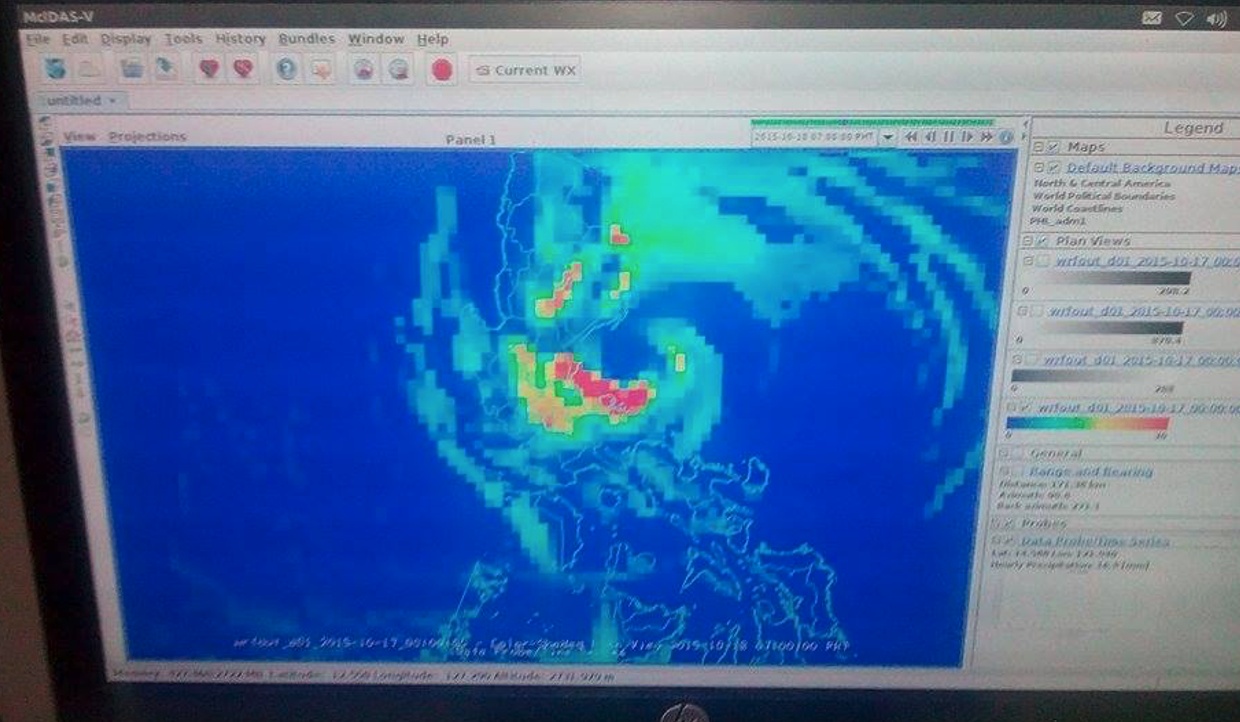
\includegraphics[keepaspectratio]{kuviot/saaennusteanimaatio.png}}

}

\caption{\label{fig-saaennusteanimaatio.png}Simulaatiomalli, jonka
avulla hurrikaanin voimaa ja liikkumista pystyttiin ennakoimaan.
(Wikimedia Commons)}

\end{figure}%

Kuten sääilmiöitä, myös liiketoimintaprosesseja voidaan tuntea
syvällisellä tasolla. Kun vaikkapa jokin valmistavan teollisuuden tai
sairaalan päivystyksen prosessi tunnetaan riittävän hyvin, voidaan myös
sen etenemistä simuloida. Emme juurikaan voi vaikuttaa sääilmiöihin,
mutta liiketoimintaprosesseihin on mahdollista vaikuttaa.

Liiketoimintaprosessien simulointi onnistuu useilla
prosessimallinnusvälineillä ja simulointiin erikoistuneilla
ohjelmistoilla. Simulointi mahdollistaa prosessimallien ''koeajamisen''.
Prosessin tehtäville, tapahtumille ja vaikkapa niiden aikana tehtäville
päätöksille voidaan määritellä todennäköisyys, kesto tai kestoväli,
kustannus tai kustannusväli ja niin edelleen. Jos prosessin aikana
kutsutaan jotain ulkoista järjestelmäpalvelua, mikä on palvelun
vasteaika arkisin ja viikonloppuisin, keskipäivällä ja yöllä? Paljonko
virheistä johtuvaa raaka-ainehukkaa voitaisiin vähentää pidentämällä
prosessin jonkin tehtävän kestoa ja maksaisiko se itsensä takaisin
suhteessa tuotannon hidastumiseen? Paljonko vuodessa voitaisiin säästää,
jos prosessin kutsuman palvelun vasteajasta saataisiin nipistettyä
sekunti pois yhtä kutsua kohden tai jos jotain manuaalista tehtävää
prosessissa suorittavat työntekijät lähetetään kahdeksi päiväksi
kouluttautumaan?

Riittävän monta simulaatioajoa voi paljastaa prosessista pullonkauloja
ja kehittämiskohteita, ja kenties jopa aivan ilmeisiä virheitä.
Prosessikulkua voidaan mallin tasolla vaivatta muuttaa, parametrien
arvoja säätää ja tarkkailla näiden vaikutuksia prosessin keskimääräiseen
toteutumaan.

\subsection{Toimintatapojen
kehittäminen}\label{toimintatapojen-kehittuxe4minen}

Monet yrityksissä ja organisaatioissa suoritettavat tehtävät ovat
muodostuneet työntekijöille rutiineiksi. Niitä suoritetaan ilman, että
tekemistä ja sen tapaa pysähdyttäisiin koskaan sen tarkemmin miettimään.
Tavallista on sekin, että jokaisen samaa tehtävää suorittavan
työntekijän rutiinit voivat hieman poiketa toisistaan. Kukaan ei siis
välttämättä tee samaa tehtävää tai suorita samaa prosessia täsmälleen
samalla tavalla kuin kollegansa.

On ilmeistä, että jotkin tavat suorittaa prosessi ovat nopeampia tai
tuottavat vaikkapa vähemmän virheitä kuin toiset. Jokin tapa toteuttaa
asiakaspalveluun liittyviä toimintoja koetaan asiakkaiden taholla
varmasti paremmaksi kuin jokin toinen. Järkevää tietysti olisi, että
jokainen työntekijä toimisi juuri sillä parhaaksi todetulla tavalla.
Prosessien tunteminen mahdollistaa niihin liittyvien parhaiden
käytänteiden dokumentoinnin ja näkyväksi tekemisen.

Paitsi toiminnan tehokkuuden kannalta, prosessien tuntemisesta ja
dokumentoimalla näkyväksi tekemisestä on myös muita hyötyjä. Yrityksen
tavoitellessa laatusertifikaattia, prosessit tulee pystyä esittämään
laatuauditoijalle. Laadukas graafinen prosessimalli tai
prosessikäsikirja eivät vielä takaa laadukasta toimintaa, vaan toiminnan
täytyy myös tapahtua prosessin mukaisesti. Laatuauditoinneissa
havainnoidaankin myös toimintaa käytännön tasolla ja henkilöstöä voidaan
haastatella, suoraan tai epäsuorasti, prosesseihin liittyen. Kokeesta
voi selvitä täysin pistein vain silloin, kun prosessit ovat paitsi
kunnossa, ne myös tunnetaan. Lisäksi prosessimallit ovat erinomainen osa
uuden henkilöstön perehdytyspakettia, ja konkareidenkin saattaa olla
joskus tarpeen tarkistaa, kuinka jokin asia tulikaan tehdä.

\subsection{Kustannussäästöt}\label{kustannussuxe4uxe4stuxf6t}

Kustannussäästöjen mahdollisuuksia voidaan löytää arvioimalla prosessiin
liittyvää hukkaa. Karkeasti yleistäen kaikki sellainen toiminta, joka ei
tuota arvoa, tulisi pyrkiä karsimaan pois.

Radikaaleimpia toimenpiteitä prosessihukan karsimiseksi ovat kokonaisten
toiminta- tai prosessialueiden alasajot. Kevyempi, joskin käytännössä
lähes yhtä radikaali toimenpide, on prosessialueiden yhdistäminen.
Mikäli esimerkiksi jokin toiminto tai toimintojen kokonaisuus on
välttämätön ydintoiminnan kannalta, mutta sen ei katsota oikeuttavan
olemassaoloaan erillisenä yksikkönä tai osastona, saatetaan
toimintokokonaisuus ja siihen liittyvät prosessit yhdistää jonkin toisen
yksikön toimintojen kanssa.

Voi myös olla niin, että samoja prosesseja toteutetaan useissa
yksiköissä. Esimerkkinä voidaan ajatella yritystä, jossa kirjanpitoa
tehdään jokaisessa yksikössä ja vieläpä erillisiä ohjelmistoja käyttäen.
Joskus tällainen voi olla perusteltua, mutta usein toiminto olisi
järkevämpää keskittää. Palvelukeskukseen keskitetty kirjanpito
mahdollistaa kustannussäästöjä skaalaetujen, yhtenäisen
ohjelmistoratkaisun ja pienempien henkilöstökulujen kautta.
Palvelukeskuksen käsittelemät suuret datamäärät voivat myös mahdollistaa
esimerkiksi ohjelmistorobotiikan ja tekoälyratkaisujen tehokkaamman
käytön. Keskitetty kirjanpito tekee mahdolliseksi myös prosessien
standardoinnin ja erikoistunut osaaminen pienentää virheriskiä.

Keskittämisen seurauksena palvelun laadun saatetaan kuitenkin kokea
laskevan. Laatu toki saattaakin laskea, esimerkiksi suhteellisesti
niukempien resurssien vuoksi. Tavallisesti prosessiasiantuntijuuden
keskittäminen kuitenkin tosiasiassa parantaa palvelujen laatua ja myös
tukee toiminnan jatkuvaa parantamista.

Koettu laadun lasku johtuu siitä, että keskitetty palvelukeskus tuottaa
palvelut vakioiduilla tavoilla ja parhaiksi tunnistettuja käytänteitä
soveltaen. Tämä voi aiheuttaa prosessien ja kulttuurien
yhteentörmäyksen. Keskitetyt prosessit eivät välttämättä olekaan
yhteensopivia niiden oletusten tai toimintatapojen kanssa, joita
palveluja käyttävissä asiakasyksiköissä on totuttu noudattamaan. Mikäli
prosessitarkastelua ei ole tehty, eikä prosessien uudistamista
suunnitella koko organisaatiota leikkaavasti, on epäonnistumisen
mahdollisuus olemassa. Haaste kasvaa, mikäli organisaation sisäisten
toimintojen uudelleenjärjestelyn sijaan kyse onkin esimerkiksi
kokonaisesta yritysfuusiosta.

Schönreiterin (2018) julkaisemassa kirjallisuuskatsauksessa todetaan,
että tutkimuskirjallisuudessa ei juurikaan käsitellä yritysfuusiota
seuraavan integraation ja liiketoimintaprosessien harmonisoinnin välistä
yhteyttä. Tämä on huomionarvoista ja yllättävääkin, koska esimerkiksi
tietojärjestelmien ja teknologioiden integraatiosta \emph{post mergers}
-tapauksissa on kirjoitettu paljonkin. Onnistunut yritysfuusio vaatii
kuitenkin onnistunutta prosessien yhteensovittamista, mikä
luonnollisesti edellyttää prosessien tuntemista.

Myös simulointi ja erityisesti prosessien mittaaminen, jota käsitellään
myöhemmin, voivat paljastaa potentiaalisia säästökohteita.

\subsection{Tiedonhallinta ja
turvallisuus}\label{tiedonhallinta-ja-turvallisuus}

Prosessien tunteminen on tarpeen myös tietoturvan, -suojan ja
tiedonhallinnan kannalta. Tiedon suojaaminen helpottuu -- tai voisi ehkä
jopa sanoa, että on mahdollista ainoastaan -- kun tiedetään, mitä tietoa
prosesseissa liikkuu ja minne. Suurennuslasin alla tässä ovat prosessit,
joissa käsitellään henkilötietoja, liiketoimintakriittistä tai salassa
pidettävää tietoa. Suomen tiedonhallintalaki\sidenote{\footnotesize Laki julkisen
  hallinnon tiedonhallinnasta,
  https://www.finlex.fi/fi/lainsaadanto/saadoskokoelma/2019/906}
edellyttää julkisia toimijoita laatimaan tiedonhallintamallin, jolta
vaaditaan muun muassa seuraavaa: ''\emph{Toimintaprosessien kuvaaminen
tiedonhallintamallissa antaa tiedonhallintayksikölle kokonaiskuvan
siitä, missä ja miten viranomaisten tieto muodostuu ja miten sitä
käsitellään. Toimintaprosessien osalta kuvataan myös niiden liittymät
toisiinsa. Toimintaprosessien osalta kuvataan liittymät myös ulkoisiin
toimintaprosesseihin.}''\sidenote{\footnotesize Suositus tiedonhallintamallista,
  Valtiovarainministeriön julkaisuja 2024:22} Onpa kentältä usein myös
kuulunut, että yritysten, jotka tunsivat ja olivat dokumentoineet
liiketoimintaprosessinsa, oli huomattavasti helpompi ryhtyä toteuttamaan
Euroopan unionin yleisen tietosuoja-asetuksen\sidenote{\footnotesize https://eur-lex.europa.eu/legal-content/FI/TXT/HTML/?uri=CELEX:32016R0679}
vaatimuksia ja rekisteröidyn henkilön tietopyyntöön vastaaminen tuotti
vähemmän päänvaivaa.

Prosessien tunteminen auttaa parantamaan myös toiminnan fyysistä ja
psykologista turvallisuutta erilaisissa tehtävissä ja tilanteissa. Näitä
aihepiirejä ei kuitenkaan tässä käsitellä.

\subsection{Toiminnan kriittisyys}\label{toiminnan-kriittisyys}

Edellä prosessin todettiin olevan toistuvaa tekemistä. Jos toiminnan
tehokkuutta ja tuloksellisuutta halutaan parantaa prosesseja
kehittämällä, ei välttämättä tunnu mielekkäältä keskittyä sellaiseen
toimintaan tai tehtäväsarjoihin, jotka toteutuvat vain harvoin.

Prosessitarkastelussa ja prosessien kehittämisessä tavallisesti
kannattaakin ensisijaisesti keskittyä niihin prosesseihin, jotka
toistuvat usein. Ne todennäköisesti liittyvät organisaation
ydintoimintaan ja toistuvuudesta seuraa vähintään se, että niihin
liittyy kumulatiivista säästöpotentiaalia.

Prosessitarkastelu kannattaa kuitenkin kohdistaa myös sellaisiin
toimintoihin, jotka ovat jollain tavalla kriittisiä. Harva yritys tai
organisaatio joutuu toistuvasti vaikkapa vakavan kyberhyökkäyksen
kohteeksi. Koska tällainen tapahtuma ei ole toistuva -- pikemminkin
harvinainen -- ei toistuvuusvaatimuksen mukaan olisi tarpeen tarkastella
prosessina sitä, kuinka kyberhyökkäyksestä seuraava tilanne saadaan
hallintaan. Sama koskee yleisemminkin kriisitilanteiden hallintaa ja
esimerkiksi kriisiviestintää. Kriisitilanteet ovat harvinaisia, eivätkä
monet organisaatiot välttämättä koskaan sellaiseen joudu. Tämä ei
kuitenkaan tarkoita sitä, etteikö niihin olisi syytä varautua.

Kyberpuolustautumisen strategiat seikkaperäisillä tilanne- ja
toimintasuunnitelmilla tarkennettuina, samoin kuin jatkuvuussuunnittelu
yleisemmin, ovat nykyisin arkipäivää lähes kaikkialla. Nämä suunnitelmat
usein sisältävät myös jonkinlaisia prosessimuotoisia toimenpidesarjoja.
Herbane ym. (2004) kirjoittavat, että ''\emph{liiketoiminnan jatkuvuuden
hallinta (Business Continuity Management, BCM) on noussut monilla
toimialoilla järjestelmälliseksi prosessiksi {[}ja{]} sen onnistumisen
kannalta oleellista on {[}\ldots{]} työntekijöiden toiminta
palautumisprosessin (business recovery process) aikana. {[}\ldots{]}
Liiketoimintaprosessien asiantuntijoiden tulisi ottaa omistajuus ja
vastuu jatkuvuuden hallinnan tehtävistä keskitetyn BCM-tiimin
koordinoivassa ohjauksessa.}\sidenote{\footnotesize Käännetty englannin kielestä.}''

Vaikka prosessi toisaalla määriteltäisiinkin usein toistuvaksi
tapahtumasarjaksi, prosessiksi kannattaa mieltää myös harvemmin -- tai
ei välttämättä edes koskaan -- tapahtuvat tapahtumasarjat, mikäli ne
ovat kriittisyydeltään merkittäviä. Ajatus lähestyy riskimatriisia --
yhtä riskien hallinnan perustyökaluista. Siinä riskit luokitellaan
tapahtuman todennäköisyyden ja tapahtuman seurausten vakavuuden
perusteella (Taulukko~\ref{tbl-riskimatriisi}).

\begin{longtable}[]{@{}
  >{\raggedright\arraybackslash}p{(\linewidth - 6\tabcolsep) * \real{0.2209}}
  >{\raggedright\arraybackslash}p{(\linewidth - 6\tabcolsep) * \real{0.2442}}
  >{\raggedright\arraybackslash}p{(\linewidth - 6\tabcolsep) * \real{0.2442}}
  >{\raggedright\arraybackslash}p{(\linewidth - 6\tabcolsep) * \real{0.2674}}@{}}
\caption{Riskimatriisi}\label{tbl-riskimatriisi}\tabularnewline
\toprule\noalign{}
\begin{minipage}[b]{\linewidth}\raggedright
Todennäköisyys
\end{minipage} & \begin{minipage}[b]{\linewidth}\raggedright
Vähäinen seuraus
\end{minipage} & \begin{minipage}[b]{\linewidth}\raggedright
Haitallinen seuraus
\end{minipage} & \begin{minipage}[b]{\linewidth}\raggedright
Vakava seuraus
\end{minipage} \\
\midrule\noalign{}
\endfirsthead
\toprule\noalign{}
\begin{minipage}[b]{\linewidth}\raggedright
Todennäköisyys
\end{minipage} & \begin{minipage}[b]{\linewidth}\raggedright
Vähäinen seuraus
\end{minipage} & \begin{minipage}[b]{\linewidth}\raggedright
Haitallinen seuraus
\end{minipage} & \begin{minipage}[b]{\linewidth}\raggedright
Vakava seuraus
\end{minipage} \\
\midrule\noalign{}
\endhead
\bottomrule\noalign{}
\endlastfoot
Epätodennäköinen & Merkityksetön riski & Vähäinen riski & Kohtalainen
riski \\
Mahdollinen & Vähäinen riski & Kohtalainen riski & Merkittävä riski \\
Todennäköinen & Kohtalainen riski & Merkittävä riski & Sietämätön
riski \\
\end{longtable}

Jääköön kontekstissa harkittavaksi, onko toiminto syytä määritellä
prosessiksi silloin, kun siihen liittyy vähäinen riski vai vasta
silloin, kun riski on kohtalainen. Riskin pienuudesta huolimatta
yllättäviin tilanteisiin, jotka voivat esimerkiksi vaurioittaa
organisaation julkisuuskuvaa, on kuitenkin syytä varautua huolellisella
prosessisuunnittelulla ja sen mahdollistamalla nopealla toimintakyvyllä.

Toimintojen kriittisyyttä, tai vaikkapa jatkuvuuteen liittyviä
vaatimuksia, voidaan arvioida useista näkökulmista. Joitain
sovellettavia arviointikriteereitä ovat esimerkiksi seuraavat
(Taulukko~\ref{tbl-kriittisyys}).

\begin{longtable}[]{@{}
  >{\raggedright\arraybackslash}p{(\linewidth - 2\tabcolsep) * \real{0.3571}}
  >{\raggedright\arraybackslash}p{(\linewidth - 2\tabcolsep) * \real{0.6429}}@{}}
\caption{Esimerkkejä toiminnon kriittisyyden arvioinnissa
sovellettavista kriteereistä}\label{tbl-kriittisyys}\tabularnewline
\toprule\noalign{}
\begin{minipage}[b]{\linewidth}\raggedright
Kriteeri
\end{minipage} & \begin{minipage}[b]{\linewidth}\raggedright
Arviointikysymys
\end{minipage} \\
\midrule\noalign{}
\endfirsthead
\toprule\noalign{}
\begin{minipage}[b]{\linewidth}\raggedright
Kriteeri
\end{minipage} & \begin{minipage}[b]{\linewidth}\raggedright
Arviointikysymys
\end{minipage} \\
\midrule\noalign{}
\endhead
\bottomrule\noalign{}
\endlastfoot
Vaikutus liiketoimintaan & Kuinka merkittävä on vaikutus
liiketoimintaan? \\
Taloudelliset seuraukset & Kuinka suuria taloudellisia tappioita
seuraa? \\
Asiakasvaikutukset & Kuinka vakavasti asiakkaat kärsivät? \\
Sääntely ja lakisääteiset vaatimukset & Liittyykö velvoitteita
lainsäädännön tai sääntelyn näkökulmasta? \\
Mainevaikutukset & Kuinka suuri mainehaitta syntyy? \\
Toipumisaika & Kuinka nopeasti toiminnon on oltava palautettavissa
normaaliksi? (esim. alle viikko, alle vuorokausi, alle tunti) \\
Tiedonmenetyksen sietokyky & Kuinka paljon toimintoon liittyvää tietoa
voidaan menettää ilman vakavia seurauksia? (esim. päivien ajalta,
tuntien ajalta, ei lainkaan) \\
\end{longtable}

\subsection{Toiminnan ja informaatioteknologian
yhteensovittaminen}\label{toiminnan-ja-informaatioteknologian-yhteensovittaminen}

Nykyisin hyvin harva liiketoimintaprosessi on täysin manuaalinen;
useimpien tukena käytetään joitain tietojärjestelmiä ja teknologioita.
Kehitettäessä tai hankittaessa uusia järjestelmiä, prosessit ovat
merkittävä osa vaatimusmäärittelydokumentaatiota (Cardoso ym. 2009;
Panayiotou ym. 2015). Toisaalta jos valmiina ostetun järjestelmän
käyttöönotto edellyttää nykyisten prosessien mukauttamista -- mikä usein
onkin tarpeen (Finney ja Corbett 2007) -- sitä luonnollisesti helpottaa,
kun prosessit tunnetaan. Tällaisessa tapauksessa prosessituntemus
mahdollistaa myös hyvin perusteltujen päätösten tekemisen siitä, mitkä
nykyisistä prosesseista ovat sellaisia, että ne halutaan säilyttää,
vaikka sitten järjestelmän räätälöinnin kalliilla kustannuksilla, ja
toisaalta mitkä ovat sellaisia, että ne voidaan muuttaa vastaamaan
järjestelmään ohjelmoituja käytänteitä. Tutkimuksissa (Finney ja Corbett
2007) on todettu, että epäonnistuneiden järjestelmäkäyttöönottojen
taustalta usein löytyy heikko prosessituntemus, epäonnistunut
prosessivaatimusten viestintä järjestelmän toimittajalle, tai
haluttomuus tai kyvyttömyys (kumpi onkaan syy ja kumpi seuraus)
mukauttaa liiketoimintaprosesseja\sidenote{\footnotesize https://www.panorama-consulting.com/lidl-erp-failure/}
järjestelmän käyttöönoton yhteydessä.

Vaikka digitaalisen transformaation voidaan katsoa käynnistyneen jo
1960- ja 1970-lukujen vaihteessa, on muutoksen vauhti edelleen
jatkuvasti kiihtyvä. Teknologiset disruptiot -- kuten vielä hyvin
muistissa oleva suuriin kielimalleihin nojaavien ja muiden
generatiivisten tekoälyjen ilmaantuminen suuren yleisön tietoisuuteen
lähes kirjaimellisesti yhdessä yössä -- edellyttävät organisaatioilta,
ja erityisesti johtamisen prosesseilta, jatkuvaa varpaillaan pysyttelyä.
Prosessit ja niiden tuottamat palvelut digitalisoituvat, halusivatpa
asiakkaat sitä tai eivät. Uudet teknologiat toisaalta tarjoavat
liiketoiminnan ja prosessien toteuttamiselle täysin uudenlaisia
mahdollisuuksia, toisaalta teknologinen kehitys useissa tapauksissa myös
pakottaa prosesseja muuttumaan. Toiminnan täytyy pysyä kiinni
kehityksessä, ja mikäpä siinä helpottaisi enemmän kuin se, että nykyinen
toiminta tunnetaan ja on siten valmis johdettavaksi kohti muutoksia.

Davenport ja Short esittivät jo vuonna 1990 (Davenport ja Short 1990),
että informaatioteknologian ja prosessien suunnittelun suhteen tulisi
olla rekursiivinen. Prosessien tarpeet toimivat lähtökohtana
IT-kyvykkyyksien kehittämiselle, ja samaan aikaan IT:n tarjoamien
mahdollisuuksien tulisi toimia syötteenä prosessien suunnittelulle ja
jopa radikaalille kokonaisvaltaiselle uudelleensuunnittelulle. Tähän
aiheeseen palataan vielä myöhemmin.

\subsection{Monimutkaisuuden hallinta}\label{monimutkaisuuden-hallinta}

Prosessiajattelu ja toimintojen mallintaminen prosesseiksi tarjoavat
apuvälineitä monimutkaisuuden hallintaan. Monimutkaisia toimintoja
luonnehtivat esimerkiksi tehtävien väliset epäselvät riippuvuudet,
toiminnan ennakoimattomuus, korkea virhealttius sekä hallinnan vaikeus.

Monimutkaisiin toimintoihin liittyy tavallisesti myös useita rooleja,
vaiheita, päätöksentekopisteitä ja riippuvuuksia. Prosessimallinnus
tekee näkyväksi mitä toiminnossa tapahtuu, missä järjestyksessä ja
miksi. Samoin se paljastaa, kuka tekee mitä ja kuinka tieto ja
materiaalit liikkuvat. Harmon (2019) on todennut, että mitä
kompleksisempi toiminto on, sitä suurempi hyöty prosessimallinnuksella
ja -analyysilla voidaan saavuttaa. Ne vähentävät monitulkintaisuutta ja
paljastavat riippuvuuksia. Riippuvuuksia voidaan tarkastella esimerkiksi
resurssi- ja aikariippuvuuksina -- esimerkiksi myöhemmin käsiteltävän
kriittisen polun menetelmän avulla.

Prosessimallit toimivat puolueettomana, esitysteknisesti neutraalina
yhteisenä viitekehyksenä ja organisaation jaettuna muistina. Ne tukevat
oppimista ja perehdytystä, pienentävät kognitiivista kuormitusta,
vähentävät virheitä, paljastavat kehittämiskohteita ja helpottavat
päätöksentekoa.

\bookmarksetup{startatroot}

\chapter{Prosessitiedon
kerääminen}\label{prosessitiedon-keruxe4uxe4minen}

Prosesseja koskevan tiedon jatkuva kerääminen on oleellista prosessien
hallinnan ja kehittämisen kannalta. Omanlaisensa ponnistus on
prosessitiedon kerääminen silloin, kun toistaiseksi dokumentoimattomat
tai kenties jopa tunnistamattomat prosessit on tarpeen saada haltuun ja
mallinnetuiksi. Prosessitiedon keräämisessä voidaan hyödyntää useita
erilaisia keinoja ja lähteitä: eksplisiittinen tieto dokumentoiduista
lähteistä, työntekijöiden hiljainen tieto eli \emph{tacit knowledge}
(ks. Nonaka ym. 1996), tietojärjestelmistä saatava data, kuten loki- ja
tapahtumatiedot sekä erilaisilla asiakaskyselyillä ja organisaation
sisäisistä ja ulkoisista sidosryhmäpalautteista saatava tieto.
Yleisimpiä keinoja prosessitiedon keräämiseen ovat haastattelut,
työpajat, havainnointi, dokumenttianalyysi ja prosessianalytiikka.

\section{Prosessien kypsyystaso ja sen
mittaaminen}\label{prosessien-kypsyystaso-ja-sen-mittaaminen}

Ennen kuin prosesseja ryhdytään kehittämään, on tarpeen tietää, mikä
niiden taso tällä hetkellä on. Kypsyysmalli (\emph{maturity model}) on
tähän tarkoitettu arviointikehikko, joka kuvaa portaittaisen
kehityspolun epämuodollisesta ja ehkä sattumanvaraisestakin toiminnasta
kohti hallittua, mitattua ja jatkuvasti parannettavaa toimintaa.
Kypsyysarviointi on siten yksi prosessitiedon keräämisen tapa: se
tuottaa jäsennellyn kuvan prosessien nykytilasta ja auttaa asettamaan
kehittämiselle realistisen tavoitetason.

Prosessien yhteydessä kypsyysmalleja käytetään tyypillisesti kolmeen
tarkoitukseen (Röglinger ym. 2012):

\begin{itemize}
\tightlist
\item
  Kuvaileva käyttö, jossa selvitetään nykytila ja tunnistetaan vahvuudet
  ja puutteet.
\item
  Ohjaava käyttö, jossa määritellään tavoitetaso ja toimenpiteet sen
  saavuttamiseksi.
\item
  Vertaileva käyttö, jossa organisaation tai yksikön tilannetta
  verrataan -- \emph{benchmarkataan} -- muihin.
\end{itemize}

Kypsyydestä puhuttaessa on syytä erottaa kaksi tasoa. Prosessin kypsyys
kuvaa yksittäisen prosessin, kuten ostolaskujen käsittelyn, kykyä
tuottaa tavoiteltu lopputulos johdonmukaisesti ja ennustettavasti.
Prosessinhallinnan kypsyys taas kuvaa koko organisaation kyvykkyyttä
johtaa ja kehittää prosessejaan: esimerkiksi onko prosesseille nimetty
omistajat, onko käytössä yhteiset mallinnuskäytännöt ja mittaristot ja
tukeeko organisaation kulttuuri prosessiajattelua (Röglinger ym. 2012).

Organisaatioissa voi olla yksittäisiä hyvin hallittuja prosesseja,
vaikka prosessijohtaminen kokonaisuutena olisikin kehittymätöntä.
Päinvastainen tilanne on harvinaisempi, sillä kypsä prosessien hallinta
käytännössä pakottaa prosessit kehittymään.

Useimmat kypsyysmallit pohjautuvat Carnegie Mellonin yliopiston Software
Engineering Instituten alun perin ohjelmistokehitykseen laatimaan
\emph{Capability Maturity Model} -malliin (Paulk ym. 1993) ja sen
seuraajaan \emph{CMMI}:hin (\emph{Capability Maturity Model
Integration}). Malli jakaa kypsyyden viiteen tasoon, jotka seuraavassa
taulukossa (Taulukko~\ref{tbl-kypsyystasot}) on sovitettu prosessien
kypsyystason tarkasteluun.

\begin{longtable}[]{@{}
  >{\raggedright\arraybackslash}p{(\linewidth - 4\tabcolsep) * \real{0.0800}}
  >{\raggedright\arraybackslash}p{(\linewidth - 4\tabcolsep) * \real{0.2700}}
  >{\raggedright\arraybackslash}p{(\linewidth - 4\tabcolsep) * \real{0.6500}}@{}}
\caption{CMMI-mallin
kypsyystasot}\label{tbl-kypsyystasot}\tabularnewline
\toprule\noalign{}
\begin{minipage}[b]{\linewidth}\raggedright
Taso
\end{minipage} & \begin{minipage}[b]{\linewidth}\raggedright
Nimi
\end{minipage} & \begin{minipage}[b]{\linewidth}\raggedright
Tyypillinen tilanne
\end{minipage} \\
\midrule\noalign{}
\endfirsthead
\toprule\noalign{}
\begin{minipage}[b]{\linewidth}\raggedright
Taso
\end{minipage} & \begin{minipage}[b]{\linewidth}\raggedright
Nimi
\end{minipage} & \begin{minipage}[b]{\linewidth}\raggedright
Tyypillinen tilanne
\end{minipage} \\
\midrule\noalign{}
\endhead
\bottomrule\noalign{}
\endlastfoot
1 & Lähtötaso (\emph{Initial}) & Toiminta on epämuodollista, ja
onnistuminen riippuu yksittäisistä henkilöistä. \\
2 & Hallittu (\emph{Managed}) & Prosessit on suunniteltu ja niitä
seurataan yksikkö- tai projektikohtaisesti. \\
3 & Määritelty (\emph{Defined}) & Prosessit on kuvattu ja vakioitu koko
organisaatiossa. \\
4 & Mitattu (\emph{Quantitatively Managed}) & Prosessien suorituskykyä
ohjataan mittaritiedon perusteella. \\
5 & Optimoiva (\emph{Optimizing}) & Prosesseja parannetaan jatkuvasti
mittaustiedon ja kokeilujen pohjalta. \\
\end{longtable}

Michael Hammerin \emph{Process and Enterprise Maturity Model}
(\emph{PEMM}) (Hammer 2007) arvioi kypsyyttä kahdesta suunnasta.
Yksittäisen prosessin kypsyyttä mitataan viidellä prosessin
mahdollistajalla (\emph{process enablers}): prosessin suunnittelu,
suorittajat, omistaja, infrastruktuuri ja mittarit. Organisaation
valmiutta taas mitataan neljällä yrityskyvykkyydellä (\emph{enterprise
capabilities}): johtajuus, kulttuuri, osaaminen ja hallintamalli.
Kumpikin arvioidaan nelitasoisella asteikolla. Hammerin keskeinen
havainto on, että mahdollistajat ovat toisistaan riippuvaisia: prosessi
on vain niin kypsä kuin sen heikoin mahdollistaja.

Rosemann ja de Bruin (2005) tarkastelevat kypsyysmallissaan prosessien
hallinnan kypsyyttä kuuden tekijän kautta: strateginen yhdenmukaisuus,
hallintamalli, menetelmät, tietotekniikka, ihmiset ja kulttuuri. Malli
muistuttaa, että prosessien hallinta ei ole ainoastaan
prosessimallinnuksiin tai työvälineisiin liittyvä asia. Kypsyys
edellyttää myös johdon sitoutuneisuutta ja prosessimyönteistä
kulttuuria.

Kypsyyden arvioinnissa voidaan hyödyntää tässä luvussa esiteltäviä
prosessitiedon keräämisen keinoja, erityisesti prosessihaastattelua ja
mittareita. Käytännössä arviointi etenee usein seuraavasti:

\begin{enumerate}
\def\labelenumi{\arabic{enumi}.}
\tightlist
\item
  Rajaus. Päätetään, arvioidaanko yksittäistä prosessia vai koko
  organisaation prosessinhallintaa, ja valitaan malli sen mukaan.
\item
  Itsearviointi. Prosessin omistaja ja keskeiset toimijat arvioivat
  nykytilan mallin kriteereillä, esimerkiksi kyselylomakkeella.
\item
  Näytön kerääminen. Itsearviota täydennetään haastatteluilla,
  työpajoilla ja dokumenttianalyysilla. Prosessilouhinta voi tarjota
  objektiivista näyttöä esimerkiksi siitä, noudatetaanko vakioituja
  prosesseja myös käytännössä.
\item
  Tason määrittäminen. Tulokset kootaan ulottuvuuksittain. Kokonaistason
  sijaan kannattaa tarkastella profiilia, joka korostaa heikkoja
  ulottuvuuksia.
\item
  Tavoitetason ja toimenpiteiden määrittäminen. Määritellään, mikä taso
  on kyseiselle prosessille tarkoituksenmukainen, ja mitä sen
  saavuttaminen edellyttää.
\item
  Uusinta. Arviointi toistetaan esimerkiksi vuosittain, jotta kehitystä
  voidaan seurata.
\end{enumerate}

\section{Kyvykkyyskartta}\label{kyvykkyyskartta}

Kyvykkyys (\emph{business capability}) on organisaation kyky, joka sillä
on tai jonka se voi hankkia saavuttaakseen tietyn lopputuloksen (The
Open Group 2022). Kyvykkyys kuvaa, mitä organisaatio pystyy tekemään,
riippumatta siitä, kuka työn tekee, millä prosesseilla tai millä
tietojärjestelmillä. Prosessi puolestaan kuvaa, miten työ tehdään.
Kyvykkyys rakentuu siis ihmisten, prosessien, tiedon ja teknologian
yhdistelmästä, ja yhtä kyvykkyyttä voi toteuttaa useampi prosessi.

Seuraavassa kuviossa (kuva~\ref{fig-kyvykkyyskartta}) on esimerkki
kyvykkyyskartasta, joka voi myös auttaa tunnistamaan kyvykkyyksiin
liittyvät ja kyvykkyyksiä toteuttavat prosessit. Kyvykkyyksien kypsyyttä
voidaan arvioida samalla tavalla kuin prosessien. Kun kartta väritetään
``lämpökartaksi'' kypsyystason tai tunnistetun parannustarpeen mukaan,
siitä näkee nopeasti, mihin kyvykkyyksiin ja niitä toteuttaviin
prosesseihin kehittämistoimet kannattaa ensimmäiseksi kohdistaa.

\begin{figure}

\centering{

\pandocbounded{\includegraphics[keepaspectratio,alt={Esimerkki kyvykkyyskartasta.}]{index_files/mediabag/kuviot/kyvykkyyskartta.pdf}}

}

\caption{\label{fig-kyvykkyyskartta}Esimerkki
kyvykkyyskartasta\sidenote{\footnotesize https://www.hosiaisluoma.fi/}}

\end{figure}%

\section{Business Model Canvas}\label{business-model-canvas}

Osterwalderin (2004) esittelemä \emph{Business Model Canvas}\sidenote{\footnotesize https://www.strategyzer.com/library/the-business-model-canvas}
(\emph{BMC}) (kuva~\ref{fig-bmc}) on laajasti käytetty strategisen
organisaatiosuunnittelun työväline. BMC voi toimia tehokkaana välineenä
myös liiketoimintaprosessien tarkastelussa, sillä se kyvykkyyskartan
tavoin tarjoaa kokonaisvaltaisen kuvan yrityksen -- tai miksei myös
julkisen tai voittoa tuottamattoman organisaation -- toiminnasta ja
auttaa yhdistämään strategisen suunnittelun operatiivisiin toimintoihin.

\begin{figure}

\centering{

\pandocbounded{\includegraphics[keepaspectratio,alt={Business Model Canvas}]{index_files/mediabag/kuviot/bmc.pdf}}

}

\caption{\label{fig-bmc}Business Model Canvas. CC BY-SA 3.0, Strategyzer
AG}

\end{figure}%

BMC-viitekehys on varsin yksinkertainen. Siinä on yhdeksän lohkoa, jotka
esittävät liiketoiminnan keskeisiä rakenneosia:

\begin{itemize}
\tightlist
\item
  Arvolupaus (\emph{Value Proposition}): Mitä arvoa yritys tuottaa
  asiakkaalle? Minkä ongelman se ratkaisee tai minkä tarpeen täyttää?
\item
  Asiakassegmentit (\emph{Customer Segments}): Kenelle arvoa tuotetaan
  ja mitkä ovat yrityksen tärkeimmät asiakasryhmät?
\item
  Kanavat (\emph{Channels}): Missä asiakkaat tavoitetaan? Kuinka arvo
  toimitetaan?
\item
  Asiakassuhteet (\emph{Customer Relationships}): Kuinka asiakkaita
  hankitaan, kuinka asiakkaat saadaan pidettyä ja kuinka asiakaskuntaa
  kasvatetaan?
\item
  Tulovirrat (\emph{Revenue Streams}): Mistä tulot saadaan? Mistä
  asiakkaat haluavat maksaa ja miten?
\item
  Ydinresurssit (\emph{Key Resources}): Mitä resursseja tarvitaan
  arvolupauksen toteuttamiseen?
\item
  Ydinaktiviteetit (\emph{Key Activities}): Mitä täytyy tehdä, jotta
  yrityksen antama arvolupaus voidaan toteuttaa?
\item
  Kumppanit (\emph{Key Partnerships}): Ketkä ovat yrityksen tärkeimmät
  yhteiskumppanit ja toimittajat?
\item
  Kustannusrakenne (\emph{Cost Structure}): Missä ja miten kustannukset
  syntyvät? Mitkä ovat suurimmat kulut?
\end{itemize}

Vaikka BMC sinällään onkin yksinkertainen ryhmittely liiketoiminnan
kannalta oleellisista asioista, voi kehyksen täyttäminen vaatia
työpajan, jos toisenkin. BMC:n esittämä teemoittelu saattaa kuitenkin
tuntua luontevammalta kuin liiketoiminnan jäsentely suoraan kyvykkyys-
tai prosessikartan muotoon.

Jo teemojen otsikoista nähdään, että BMC voi monella tapaa tukea
prosessien tunnistamista, niiden hallinnan suunnittelua ja kehittämistä.
Jokaisen teeman kohdalla voidaan esittää kysymykset: Mitä prosesseja
tähän liittyy ja kuinka ne toimivat? Esimerkiksi: Mitkä prosesseista
ovat välttämättömiä asiakkaille annettavan arvolupauksen
toteuttamiseksi? Jos arvolupaus on nopea toimitus, on prosesseissa
tietenkin painotettava logistiikan tehokkuutta. Ovatko prosessit
optimoitu erilaisten asiakasryhmien tarpeisiin? Millä prosesseilla
toteutetaan asiakashankintaa ja kuinka ne toimivat? Ovatko arvolupauksen
toteuttamisen kannalta olennaisiksi todetut ydinaktiviteetit (eli
ydinprosessit) riittävästi resursoituja? Voidaanko kustannusrakenteita
keventää prosesseja tehostamalla tai olisiko syytä harkita prosessien
ulkoistamista? Ja niin edelleen.

Kun kanvaasi on täytetty, voidaan jokaisen alueen sisältö vielä
järjestää prioriteettijärjestykseen. Mikä asiakasryhmistä tai
asiakkuuksista on tärkein? Mitä uutta asiakasryhmää voitaisiin
tavoitella? Mistä suurin tulovirta saadaan nyt? Entä mistä se tulee
kolmen vuoden kuluttua? Mitkä ydinaktiviteeteista ovat kaikista
tärkeimmät? Missä syntyvät toiminnan suurimmat kustannukset?
Priorisoinnin avulla kehitystyötä voidaan suunnata ja muutoksen
laajuutta rajata.

Priorisoinnin jälkeen kanvaasin avulla voidaan myös tarkastella eri
osa-alueiden prioriteettien johdonmukaisuutta. Jos välittömästi
arvolupauksen toteuttamiseen liittyvät toiminnot löytyvät
ydinaktiviteettien joukosta vasta alemmilta sijoilta, tai eivät ehkä
löydy sieltä ollenkaan, jossain on vikaa. Jos tulovirrat ja
ydinresurssit eivät kohtaa, jälleen on prosessien johtamisessa menty
metsään.

Kun liiketoimintamalli on kuvattu, voidaan arvioida, mitkä prosessit
ovat tärkeimpiä strategian toteutumiselle. Näihin prosesseihin tulee
kohdentaa resursseja ja tarvittaessa parantamistoimia. Arvolupauksen
toteutusta voidaan optimoida ja resurssien käyttöä saatetaan voida
tehostaa esimerkiksi prosessiautomaation avulla. BMC voi myös osoittaa,
mihin prosesseihin liittyvää dataa olisi tarpeen kerätä ja analysoida,
jotta liiketoimintamallia voidaan jalostaa tiedolla johtamisen avulla.

Tunnettuudestaan huolimatta BMC ei välttämättä ole ensimmäisenä mieleen
nouseva väline liiketoimintaprosessien tarkastelun tueksi, mutta se on
siihen erinomainen väline. Sen käyttö mahdollistaa prosessien
systemaattisen tarkastelun nimenomaan strategian näkökulmasta. Sitä
soveltamalla voidaan optimoida prosesseja tukemaan arvolupausta,
vähentää kustannuksia ja parantaa asiakastyytyväisyyttä. Tämä johtaa
kokonaisvaltaiseen liiketoimintaprosessien, ja siten liiketoiminnan,
kehittämiseen. BMC tarjoaa prosesseihin kuitenkin karkean, oikeastaan
vain otsikkotasoisen näkymän. Tarkastellaankin seuraavaksi joitain
keinoja ja tekniikoita, joiden avulla voidaan päästä kiinni prosessien
kulkuun ja sitä kautta kehittämisen yksityiskohtaisempiin suuntiin.

\section{Olemassa oleva
dokumentaatio}\label{olemassa-oleva-dokumentaatio}

Prosesseja koskevaa dokumentoitua tietoa voidaan löytää monista
lähteistä. Useissa yrityksissä ja organisaatioissa on työ- tai
toimintaohjeita, jotka saattavat parhaassa tapauksessa kuvata jopa askel
askeleelta, kuinka jokin tehtävä suoritetaan. Sikäli ne ovat myös väline
toiminnan jatkuvuuden varmistamiseksi esimerkiksi henkilöstömuutosten
yhteydessä. Lisäksi ne voivat liittyä toiminnan laadun varmistamiseen ja
monet laatujärjestelmät edellyttävätkin melko seikkaperäisiä
toimintakuvauksia. Kemppaisen (2018) tutkimuksessa todetaan hyvän
työohjeen olevan sellainen, jonka ''avulla pystyy suorittamaan tarkasti
määritetyn työtehtävän ilman muita ohjeita tai muuta opastusta.''
Seuraavassa (kuva~\ref{fig-matkaohje}) on katkelma erään yliopiston
työmatkaohjeesta.

\begin{figure}

\centering{

\pandocbounded{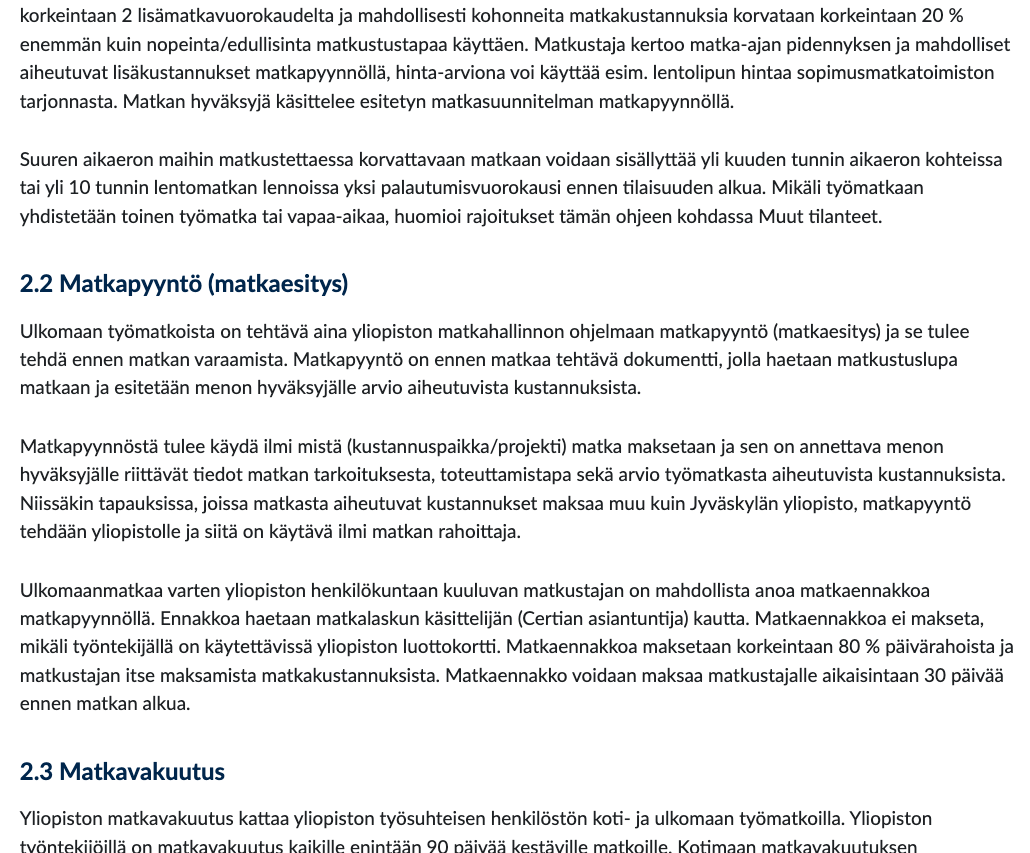
\includegraphics[keepaspectratio,alt={Katkelma yliopiston työmatkaohjeesta.}]{kuviot/matkaohje.png}}

}

\caption{\label{fig-matkaohje}Katkelma yliopiston työmatkaohjeesta}

\end{figure}%

Laatujärjestelmät, kuten ISO 9001 Laadunhallinta\sidenote{\footnotesize https://sfs.fi/standardeista/tutustu-standardeihin/suositut-standardit/iso-9001-laadunhallinta/},
edellyttävät prosessimaista toimintatapaa ja prosessien määrittämistä.
ISO 9001 Laadunhallinta -järjestelmää ohjaavia periaatteita ovat
asiakaslähtöisyys ja laadun jatkuva parantaminen, joten
laatusertifikaatin ansainneen organisaation voidaan olettaa päässeen jo
varsin pitkälle prosessiajattelussa ja prosessimuotoisessa toiminnassa.
Useissa sertifioimattomissakin organisaatioissa on laadittu
laatujärjestelmiä, vastuutauluja tai vaikkapa vähemmän muodollisia
laatukäsikirjoja, jotka voivat toimia erinomaisena materiaalina
liiketoimintaprosesseja tarkasteltaessa.

Vaikka laatukäsikirjaa ei löytyisikään, on useimmilla organisaatioilla
ainakin jonkinlainen organisaatiokaavio tehtävänimikkeineen ja
vastuualuekuvauksineen. Samoin esimerkiksi verkkosivuilla olevat
kuvaukset asiakkaille tarjottavista palveluista voivat myös johtaa
prosessien äärelle. Tietojärjestelmien käyttöohjeet ja muut niihin
liittyvät dokumentaatiot saattavat tarjota yksityiskohtaistakin tietoa
prosesseista, joita toteutetaan tai tuetaan IT-ratkaisuilla.

Sopimukset kuten palvelutasosopimus (\emph{Service Level Agreement},
\emph{SLA}), samoin kuin toimintaa koskeva lainsäädäntö tai muu
sääntely, on myös hyvä kartoittaa ja käydä ainakin keskeisiltä osiltaan
läpi. Nämä voivat paitsi tarjota tietoa nykytilan prosessien
toteutuksesta, ne asettavat myös ensimmäiset raamit uusien prosessien
suunnittelulle.

\section{Prosessihaastattelu}\label{prosessihaastattelu}

Haastattelun avulla voidaan saada syvällistä tietoa prosessien kulusta
sekä esimerkiksi resurssitarpeista, pullonkauloista ja mahdollisista
poikkeustilanteista. Haastattelua voidaan käyttää pyrittäessä nykyisten
prosessien dokumentointiin ja ymmärtämiseen. Sitä voidaan myös käyttää
tiedonkeruumenetelmänä suunniteltaessa ja määriteltäessä prosesseille
tavoitetiloja, ja siihen haastattelu onkin yksi parhaista
tiedonkeruuvälineistä. Koska haastattelu soveltuu useisiin
käyttötarkoituksiin ja se voidaan toteuttaa monessa eri muodossa, onkin
ensimmäiseksi tärkeää määritellä tavoitteet ja vasta sen jälkeen
suunnitella haastattelun toteutus.

Haastattelun päätyypit ovat strukturoitu, puolistrukturoitu ja avoin
haastattelu. Strukturoitu eli rakenteinen muoto on käytettävissä
silloin, kun jo etukäteen tarkasti tiedetään, mitä tietoa tarvitaan ja
missä muodossa se halutaan saada. Strukturoidun haastattelun
ominaisuuksia on esitetty taulukossa alla
(Taulukko~\ref{tbl-strukturoitu-haastattelu}). Suljetuilla kysymyksillä
tarkoitetaan esimerkiksi valinta- ja luokituskysymyksiä.

\begin{longtable}[]{@{}
  >{\raggedright\arraybackslash}p{(\linewidth - 2\tabcolsep) * \real{0.5000}}
  >{\raggedright\arraybackslash}p{(\linewidth - 2\tabcolsep) * \real{0.5000}}@{}}
\caption{Strukturoidun haastattelun
ominaisuudet}\label{tbl-strukturoitu-haastattelu}\tabularnewline
\toprule\noalign{}
\begin{minipage}[b]{\linewidth}\raggedright
Ominaisuus
\end{minipage} & \begin{minipage}[b]{\linewidth}\raggedright
Kuvaus
\end{minipage} \\
\midrule\noalign{}
\endfirsthead
\toprule\noalign{}
\begin{minipage}[b]{\linewidth}\raggedright
Ominaisuus
\end{minipage} & \begin{minipage}[b]{\linewidth}\raggedright
Kuvaus
\end{minipage} \\
\midrule\noalign{}
\endhead
\bottomrule\noalign{}
\endlastfoot
Kysymykset & Kysymykset ovat täsmällisesti etukäteen määriteltyjä
(suljettuja tai puoliavoimia), eikä niiden sisältöä tai muotoa varioida
haastattelun aikana tai niiden välillä. \\
Järjestys & Kysymykset esitetään samassa järjestyksessä kaikille
haastateltaville. \\
Haastattelijan rooli & Haastattelija pysyy neutraalina, ei improvisoi
eikä johdattele haastateltavaa. \\
Tavoite & Tavoitteena on kerätä määrämuotoista ja kvantifioitavaa
tietoa. \\
Dokumentointi & Vastaukset kirjataan täsmällisesti, esimerkiksi
lomakkeelle tai tietokantaan. \\
\end{longtable}

Strukturoitu haastattelu soveltuu käytettäväksi silloin, kun ei ole
tarpeen päästä kiinni prosessikulun nyansseihin, vaan tavoitteena on
muodostaa yleiskuva prosessista tai käytännöistä, ja kun halutaan saada
määrällisessä muodossa analysoitavaa tietoa esimerkiksi prosessin
kestosta, toistuvuudesta ja tehtävien suoritusjärjestyksestä.
Määrämuotoinen strukturoitu haastattelu tuottaa yhtenäistä ja
vertailtavaa aineistoa, joka on helppo kvantifioida ja analysoida. Muoto
helpottaa myös useiden haastateltujen henkilöiden vastausten vertailua.

Strukturoidulla haastattelulla ei kuitenkaan pystytä syventymään
yksittäisen haastateltavan kokemuksiin tai kontekstiin, eikä se
mahdollista joustavaa keskustelua tai lisäkysymysten esittämistä. Sen
vuoksi strukturoitu haastattelu vaatii huolellisen ennakkosuunnittelun
ja haastattelurungon testaamisen ennen haastattelujen aloittamista.

Avoin haastattelu puolestaan toteutetaan ilman valmista kysymysrunkoa ja
kysymykset muotoutuvat haastattelun edetessä. Haastattelun kulku vastaa
vapaata keskustelua ja sen tavoitteena on ymmärtää ilmiötä, eli
prosessihaastattelun tapauksessa jotain prosessia, haastateltavan
näkökulmasta ja hänen kontekstissaan. Tekniikka soveltuu käytettäväksi
parhaiten silloin, kun käsiteltävät prosessit ovat monimutkaisia tai
huonosti jäsentyneitä, tai kun ollaan nimenomaan kiinnostuneita
haastateltavien kokemuksista ja näkemyksistä. Avoin haastattelu voi olla
toimiva tekniikka esimerkiksi lähdettäessä kartoittamaan huonosti
hallussa olevia prosessialueita. Avointen haastattelujen muodossa
toteutetun ensimmäisen tiedonkeruukierroksen jälkeen on mahdollista
siirtyä systemaattisempiin tiedonkeruumenetelmiin. Vastaavasti avointa
haastattelua voidaan käyttää vaikkapa strukturoitujen tai
puolistrukturoitujen haastattelujen jälkeen eli siinä vaiheessa, kun
prosessista alkaa olla jo yleiskäsitys, mutta lisäksi halutaan vielä
selvittää toimijakohtaisia näkemyksiä tai harvinaisempia yksityiskohtia
ja poikkeustilanteita.

Puolistrukturoitu haastattelu on todennäköisesti yleisin muoto
prosessihaastatteluja toteutettaessa; ainakin se on yleisin
haastattelumenetelmä laadullisissa tutkimuksissa (Adeoye-Olatunde ja
Olenik 2021). Se yhdistää sekä strukturoidun että avoimen haastattelun
ominaisuuksia. Kysymysrunko on valmiiksi mietitty ja se voi sisältää
sekä määrämuotoisia että avoimia kysymyksiä. Haastattelija voi muuttaa
kysymysten esittämisjärjestystä ja tarvittaessa esittää tarkentavia tai
lisäkysymyksiä. Keskustelun kulku on joustava, mutta ei samalla tavalla
vapaasti rönsyilevä kuin avoimessa haastattelussa. Puolistrukturoitu
haastattelu pyrkii tuottamaan määrämuotoista tietoa, mutta mahdollistaa
kuitenkin syventävien ja haastateltavan kontekstiin liittyvien
huomioiden esille nousun. Tätä haastattelutyyppiä käytetään, kun
halutaan teemoittain vertailtavaa aineistoa, mutta samalla myös syvempää
laadullista ymmärrystä. Puolistrukturoidun haastattelun ominaisuuksia on
koottu seuraavaan taulukkoon
(Taulukko~\ref{tbl-puolistrukturoitu-haastattelu}).

\begin{longtable}[]{@{}
  >{\raggedright\arraybackslash}p{(\linewidth - 2\tabcolsep) * \real{0.5000}}
  >{\raggedright\arraybackslash}p{(\linewidth - 2\tabcolsep) * \real{0.5000}}@{}}
\caption{Puolistrukturoidun haastattelun
ominaisuudet}\label{tbl-puolistrukturoitu-haastattelu}\tabularnewline
\toprule\noalign{}
\begin{minipage}[b]{\linewidth}\raggedright
Ominaisuus
\end{minipage} & \begin{minipage}[b]{\linewidth}\raggedright
Kuvaus
\end{minipage} \\
\midrule\noalign{}
\endfirsthead
\toprule\noalign{}
\begin{minipage}[b]{\linewidth}\raggedright
Ominaisuus
\end{minipage} & \begin{minipage}[b]{\linewidth}\raggedright
Kuvaus
\end{minipage} \\
\midrule\noalign{}
\endhead
\bottomrule\noalign{}
\endlastfoot
Kysymykset & Kysymykset ovat etukäteen laadittuja, mutta niitä voidaan
muokata tilanteen ja haastateltavan aiempien vastausten mukaan. \\
Järjestys & Haastattelun teemat pyritään käymään läpi suunnitellussa
järjestyksessä, mutta järjestys ei ole tiukasti sidottu. \\
Haastattelijan rooli & Haastattelija ohjaa keskustelua ja voi esittää
lisäkysymyksiä ja tarkennuspyyntöjä joustavasti. \\
Tavoite & Tavoitteena on yhdistää laadullinen syvyys ja aineiston
vertailtavuus. \\
Dokumentointi & Haastattelut tavallisesti tallennetaan ja litteroidaan.
Vaihtoehtoisesti haastattelija voi tehdä haastattelun aikana tarkkoja
muistiinpanoja teemoittain. \\
\end{longtable}

\begin{quote}
\textbf{Seuraava osuus perustuu Sara Seppäsen kanssa käytyyn
keskusteluun prosessihaastatteluista ja prosessitiedon keräämisestä.
Seppänen toimii pääarkkitehtina ja hänellä on runsaasti kokemusta myös
prosessien kehittämisestä.}

Haastattelun tavoitteiden mukaisesti haastateltaviksi voidaan valita
esimerkiksi prosessien omistajia, asiantuntijoita, työntekijöitä tai
sidosryhmiä, joista kukin tarjoaa prosessiin erilaisen näkökulman.
Kannattaa pitää mielessä, että haastattelujen avulla saatava tieto on
aina vähintään jossain määrin subjektiivista -- myös strukturoitujen
haastattelujen tapauksessa.

Prosessin omistaja tuntee prosessinsa tavoitteen ja resurssit sekä sen,
kuinka se liittyy muihin prosesseihin ja toimintaympäristöönsä. Koska
prosessin omistajalla on kokonaiskuva prosessista, osaa hän
todennäköisesti kertoa ainakin yleisellä tasolla, mitä kaikkea
prosessiin liittyy, sekä neuvoa, ketä muita olisi tavoitteiden
saavuttamiseksi hyödyllistä haastatella.

Prosessin yksityiskohtaisemman kulun selvittämiseksi voi olla tarpeen
kääntyä prosessin operatiivisessa toteuttamisessa toimivan henkilöstön,
esimerkiksi prosessitiimin, puoleen. Jotta kaikki relevantit näkökulmat
saadaan katettua, usein tarvitaan eri toimijaryhmien haastatteluja ja
haastatteluaineistojen yhdistelemistä.

Lähellä prosessia toimiva ja prosessiin liittyviä tehtäviä toteuttava
työntekijä ei välttämättä kuitenkaan ajattele toimintaansa tai
työtehtäviään prosesseina\sidenote{\footnotesize Prosessihaastattelut voivatkin toimia
  myös hyvänä prosessiajattelun esittelyn ja jalkauttamisen välineenä.}.
Siksi haastattelijan on mietittävä, millaisia kysymyksiä hänen tulisi
esittää, jotta haastattelujen tavoitteita vastaavaa tietoa voidaan
saada. Prosessin toteuttamiseen osallistuvalla haastateltavalla saattaa
olla yksityiskohtaista tietoa joistain prosessissa usein toistuvista
tehtävistä tai ongelmakohdista. Vastaavasti jotkin muut prosessin
vaiheet tai poikkeustilanteet, jotka saattavat olla hyvinkin
merkityksellisiä, voivat tulla kuitatuiksi lyhyesti ja ainoastaan
yleisellä tasolla.

Erityisesti avoimia ja puolistrukturoituja haastatteluja tehtäessä on
tavallista, että jokainen prosessin toteuttamiseen osallistuva kertoo
prosessille hieman erilaisen kulun. Ihmiset korostavat omasta
kontekstistaan eri asioita; sellaisia, joita itse pitävät prosessin
kannalta oleellisimpina. Vaikka tällaisen aineiston yhteen vetäminen voi
olla työlästä, se mahdollistaa perusteellisen kokonaisnäkemyksen
muodostamisen, ja onkin kenties arvokkainta tietoa, mitä prosessista
voidaan saada.

On myös mahdollista, että prosessi todellakin toteutuu tapauksen ja
toteuttajan mukaan eri tavoilla, eli prosessikulku ei ole vakioitunut.
Mallinnetut kuvaukset saman prosessin erilaisista kuluista ja toteumista
ovat tärkeää materiaalia vakioituja prosessikäytänteitä suunniteltaessa
ja prosesseja kehitettäessä. Prosessin omistaja tai objektiivinen
prosessiasiantuntija voi analysoida erilaisia variantteja ja
tarkastella, kuinka ne toteuttavat prosessille asetettuja tavoitteita ja
vaatimuksia. Variaatioiden joukosta voidaan valita ideaalisin toteutus
tai erilaisista prosessikuluista voidaan poimia parhaat osat, jotka
yhdistetään vakioitavaksi prosessimuodoksi.
\end{quote}

Seuraavaksi esitetään Seppäsen toteutusmalli prosessihaastattelujen
suunnittelusta tulosten loppukatselmointiin ja prosessien jatkuvaan
kehittämiseen.

\begin{quote}
\begin{enumerate}
\def\labelenumi{\arabic{enumi}.}
\item
  \textbf{Ymmärrä työn tavoitteet}. Ensin tulee määritellä, mitä
  haastatteluilla pyritään saavuttamaan. Tavoitteena voi esimerkiksi
  olla jonkin nykyisen prosessin dokumentoiva kuvaaminen,
  automaatiomahdollisuuksien tunnistaminen tai tavoitetilan suunnittelua
  ja kehittämistä tukevan informaation kerääminen. Tavoitteen kautta
  pystytään asettamaan haastattelurunkoon sopivat teemat ja kysymykset.
  Mikäli tavoitteena on muodostaa yleinen käsitys prosesseista ja niiden
  liittymäkohdista, tulee haastattelut ja muu tiedonkeruu toteuttaa eri
  tavalla, kuin jos tavoitteena on tuottaa mahdollisimman
  yksityiskohtainen kuvaus nykyisestä prosessikulusta tai suunnitella
  parannettu tai jopa kokonaan uudistettu prosessikulku.
\item
  \textbf{Tutustu prosessiin mahdollisimman hyvin ennen haastattelujen
  aloittamista}. Seuraavaksi haastattelijan tulee tutustua kaikkeen
  relevanttiin taustamateriaaliin, kirjallisiin lähteisiin, kuten
  työohjeisiin sekä toiminnallisiin ja kenties strategisiinkin
  tavoitteisiin, mitä käsiteltävästä prosessista on saatavilla. Jos
  prosessi tuottaa palvelua asiakkaalle, tutustutaan palvelun
  kuvaukseen, joka voi löytyä yrityksen tai organisaation
  verkkosivuilta. Saatavilla voi olla myös prosessin asiakkaille
  tarkoitettuja ohjeita. Mikäli prosessi toteutetaan
  tietojärjestelmällä, voi järjestelmästä ja sen dokumentaatioista
  löytyä ainakin välillisesti prosessikulkuun liittyvää informaatiota.
  Samoin, jos prosessiin liittyy esimerkiksi lomakkeita, tulee niihin
  tutustua, ja sähköisten lomakkeiden tapauksessa niiden toimintaa
  kannattaa myös kokeilla. Näin saadaan selville, mitä informaatiota
  prosessissa käsitellään. Erilaisten taustamateriaalien avulla
  prosessista saadaan todennäköisesti luotua ensimmäinen kuvaus jo ennen
  ensimmäisenkään haastattelun toteuttamista. Mitä paremmin
  haastattelija ymmärtää prosessia jo valmiiksi, sitä tuloksellisempia
  haastattelut tulevat olemaan. Tämä paitsi säästää haastateltavien
  aikaa ja auttaa haastattelijaa esittämään oikeita kysymyksiä, se myös
  helpottaa haastatteluaineiston tulkintaa. Haastattelijalla on paremmat
  edellytykset ymmärtää, milloin vastaukset käsittelevät keskeisiä
  teemoja ja milloin ne ehkä liikkuvat lillukan varsissa.
\item
  \textbf{Tee luonnos prosessikulusta}. Usein on hyödyllistä laatia
  taustatietojen perusteella prosessikulusta ensimmäinen luonnos. Mikäli
  prosessia on tarkoitus mallintaa myös haastattelun aikana (ks. kohta
  6), voi alustava hahmotelma toimia haastattelijan muistin tukena.
\item
  \textbf{Haastattele ensimmäiseksi prosessin omistaja}. Jotta
  prosessista, sen tavoitteista ja vaatimuksista -- esimerkiksi
  prosessia koskevasta sääntelystä -- saadaan aluksi korkean tason
  käsitys, kannattaa haastattelut aloittaa prosessin omistajasta. Vaikka
  omistaja ei välttämättä tunne prosessikulun kaikkia yksityiskohtia,
  erityistapauksia tai poikkeamia, osaa hän varmasti neuvoa, ketä näiden
  osalta kannattaa haastatella seuraavaksi. Mikäli prosessilla ei ole
  nimettyä omistajaa, voidaan haastatteluun kutsua esimerkiksi
  toiminta-alueen esihenkilö.
\item
  \textbf{Valitse muut haastateltavat}. Seuraavaksi valitaan muut
  haastateltavat ja sovitaan haastattelujen aikataulu. On mahdollista,
  että joku ehdottaa itsensä sijaan haastateltavaksi jotain toista,
  tehtävän tai prosessin paremmin tuntevaa henkilöä.
\item
  \textbf{Toteuta haastattelut}. Haastattelun aluksi kannattaa käydä
  tavoitteet läpi haastateltavan kanssa: Miksi haastattelu toteutetaan.
  Mitä tarkoitusta se palvelee. Miksi juuri kyseistä henkilöä haluttiin
  haastatella. Mistä asioista haastattelija on kiinnostunut kuulemaan ja
  mikä on haastattelun tavoiteltu lopputulos. Mikäli tarpeen,
  haastateltava voidaan lyhyesti perehdyttää liiketoimintaprosesseihin
  ja niiden käsitteistöön yleisellä tasolla. Samalla voi olla
  hyödyllistä käydä läpi jokin yksinkertainen prosessikulku
  uimaratoineen esimerkiksi vuokaavion tai BPMN-mallin muodossa.
  Orientaatioksi voidaan jo ennen haastattelua toimittaa esimerkiksi
  prosessikorttipohja tai muuta materiaalia, jonka tuella haastateltava
  voi miettiä prosessia etukäteen. Sara Seppänen kuitenkin huomauttaa,
  että tällaiset ennakkomateriaalit saattavat myös hämmentää tai
  tarpeettomasti kuormittaa haastateltavaa, eikä hän itse niitä käytä.
  Prosessin dokumentointiin tähtäävän haastattelun toteuttamiseen on
  erilaisia käytänteitä. Jotkut haastattelijat ainoastaan kirjaavat
  asioita muistiin ja avaavat muistiinpanot prosessimalliksi
  haastattelun jälkeen. Seppänen kertoo usein piirtävänsä prosessimallia
  jo haastattelun aikana siten, että myös haastateltava voi nähdä sen.
  Tällöin haastateltava pystyy seuraamaan, kuinka hänen vastauksensa
  tulevat tulkituiksi prosessin muotoon ja tarvittaessa välittömästi
  korjata mahdolliset väärinymmärrykset. Samoin mallin kautta
  haastateltavan mieleen voi nousta asioita, joita hän ei ole vielä
  huomannut mainita. Lisäksi prosessimalli auttaa pitämään keskustelun
  tarkkuustason johdonmukaisena ja tavoitetta vastaavana. Vaiheittain
  rakentuvasta graafisesta mallista on helpompi huomata, mikäli
  keskustelu uhkaa ajautua tarpeettomiin yksityiskohtiin tai toisaalta
  liikkuu tavoitteisiin nähden liian yleisellä tasolla. Haastattelun
  aikana piirrettävä prosessimalli kannattaa kuitenkin pitää
  notaatioltaan yksinkertaisena. Useimpiin tilanteisiin riittävät BPMN:n
  peruselementit tai esimerkiksi vuokaaviomalli. Lopputulos haastattelun
  päättyessä on tavallisesti yleisellä tasolla esitetty prosessikulku,
  jota on höystetty joukolla yksityiskohtiin, poikkeuksiin ja tarkennus-
  tai selvitystarpeisiin liittyviä annotaatioita tai muistilappuja.
\item
  \textbf{Dokumentoi ja arvioi haastattelun tuottamat tiedot}.
  Haastattelun jälkeen muistiinpanot kirjoitetaan auki. Mikäli
  haastattelun aikana on piirretty prosessimallia, sitä tarvittaessa
  korjataan ja täydennetään muistiinpanojen avulla, viimeistellään ja
  tarkastetaan. Mikäli muistiin on kirjattu lisäselvitystä vaativia
  asioita, nämä selvitetään ensimmäiseksi. Sen jälkeen muistiinpanot ja
  / tai prosessimalli toimitetaan haastatellulle kommentoitavaksi.
  Yksinkertaisimmillaan tämän voi toteuttaa kysymällä haastatellulta,
  vastaavatko ne todellisuutta.
\item
  \textbf{Toteuta tarvittavat lisähaastattelut ja iteraatiot}.
  Haastateltava ei välttämättä osaa kertoa prosessista kuin siltä osin,
  mitä hänen omalla ''uimaradallaan'' tapahtuu. Voikin olla tarpeen
  sopia lisähaastatteluja, jotta prosessista saadaan muodostettua
  riittävän kokonaisvaltainen käsitys. Etenkin kysymykset prosessin
  käynnistymisestä, päättymisestä sekä prosessiin tulevista ja siitä
  lähtevistä tietovirroista voivat paljastaa lisää prosessiin liittyviä
  rooleja, toimijoita ja rajapintoja muihin prosesseihin. Saattaa
  esimerkiksi olla, että prosessi on itse asiassa käynnistynyt jo ennen
  kuin haastateltu henkilö osallistuu siihen tai jatkuu sen jälkeen, kun
  hänen tehtävänsä prosessiin liittyen ovat tulleet valmiiksi.
  Mahdollista on sekin, että haastattelun perusteella tunnistetaan
  erilaisia tapauksia ja prosessikulkuja, jotka todellisuudessa ovat eri
  prosesseja: esimerkiksi henkilöasiakkaan ja yritysasiakkaan prosessit.
  Joskus voi olla tarpeen kuulla haastateltuja henkilöitä vielä
  uudelleen. Usein esimerkiksi täydentävät kysymykset voidaan kuitenkin
  esittää lyhyessä lisäpalaverissa tai kommenttipyynnön yhteydessä
  kirjallisesti ilman tarvetta uudelle haastattelukierrokselle.
\item
  \textbf{Toteuta loppukatselmointi}. Lopuksi prosessimalli ja muut
  prosessista kerätyt tiedot toimitetaan prosessin omistajalle, joka
  katselmoi ja hyväksyy lopputuloksen.
\item
  \textbf{Prosessien jatkuva parantaminen}. Katselmoitu ja hyväksytty
  prosessi voidaan tarvittaessa avata uudelleen tarkasteltavaksi.
  Prosessikatselmointi on suositeltavaa toteuttaa säännöllisesti ja
  sitoa se esimerkiksi vuosikelloon. Laadunhallinnan ja prosessien
  kehittämisen kannalta tulee tietysti myös seurata prosessin toteumaa.
  Vastaako toteuma suunniteltua prosessikulkua ja vastaavatko prosessin
  tulokset asetettuja tavoitteita. Herätteenä uudelle tarkastelulle
  voivat myös toimia esimerkiksi muutokset toimintaympäristössä,
  tietojärjestelmissä tai vaikkapa lainsäädännössä, kuin myös
  merkittävät muutokset virheiden, läpimenoaikojen tai muiden
  seurattavien mittareiden tuloksissa.
\end{enumerate}
\end{quote}

Puolistrukturoitu prosessihaastattelu voisi edetä esimerkiksi
seuraavanlaisten kysymysten varassa. Puolistrukturoitua haastattelua
saatetaan kutsua myös teemahaastatteluksi. Seuraavista
esimerkkikysymyksistä on tunnistettavissa ainakin seuraavat teemat:
prosessin kulku, prosessissa käsiteltävät ja tuotettavat tiedot,
prosessissa käytettävät tietojärjestelmät, prosessin ongelmakohdat ja
prosessin kehittämismahdollisuudet. Kaikki etukäteen päätetyt teemat
pyritään käsittelemään haastattelun aikana, mutta se, missä vaiheessa
haastattelua ne käsitellään, voi tarvittaessa vaihdella. Samoin teemaan
liittyviä kysymyksiä voidaan säätää haastattelun aikana.

\textbf{\emph{Voitko kuvailla, miten prosessi etenee?}}

\begin{itemize}
\tightlist
\item
  \emph{Ketä toimijoita prosessin toteuttamiseen itsesi lisäksi
  osallistuu ja mitkä heidän roolinsa prosessissa ovat?}
\item
  \emph{Milloin prosessi käynnistyy? Mikä rooli ja tapahtuma sen
  käynnistää?}
\item
  \emph{Kuinka monta kertaa prosessi suoritetaan päivän / viikon /
  kuukauden / vuoden aikana?}
\item
  \emph{Mikä on prosessin ensimmäinen, toinen, \ldots, viimeinen
  vaihe}\sidenote{\footnotesize Vaiheella tarkoitetaan tässä BPMN-mallin mukaista
    tehtävää (\emph{Task}).}\emph{?}
\item
  \emph{Mikä on sinun vastuusi prosessin ensimmäisessä, toisessa,
  \ldots, viimeisessä vaiheessa?}
\item
  \emph{Mitä tietoja tarvitset näissä vaiheissa ja mistä saat nämä
  tiedot?}
\item
  \emph{Mitä tietoja vaiheessa syntyy ja minne nämä tiedot menevät?}
\item
  \emph{Mitä tietojärjestelmiä käytät vaiheissa ja kuinka järjestelmät
  tukevat työtäsi?}
\item
  \emph{Mitä prosessin lopputulemalta vaaditaan? Voiko prosessi
  esimerkiksi jäädä kesken tai olla tulematta valmiiksi?}
\item
  \emph{Onko prosessissa vaiheita, joissa se usein hidastuu tai törmää
  joihinkin ongelmiin?}
\item
  \emph{Mistä edelliset johtuvat?}
\end{itemize}

\textbf{\emph{Mitä virhe- tai poikkeustilanteita prosessin aikana voi
tapahtua?}}

\begin{itemize}
\tightlist
\item
  \emph{Mistä virheet tai poikkeukset johtuvat?}
\item
  \emph{Kuinka usein virheitä tai poikkeuksia tapahtuu?}
\end{itemize}

\textbf{\emph{Miten prosessia voisi mielestäsi parantaa?}}

\begin{itemize}
\tightlist
\item
  \emph{Liittyykö prosessikulkuun ongelmia tai kehittämiskohteita?}
\item
  \emph{Tukevatko tietojärjestelmät prosessin toteuttamista?}
\item
  \emph{Onko prosessi resursoitu riittävästi?}
\end{itemize}

\section{Prosessilouhinta}\label{prosessilouhinta}

Prosessilouhinta (\emph{Process Mining}) on tekniikka, jossa
tietojärjestelmien lokeja tarkastelemalla pyritään tekemään näkyväksi ja
analysoimaan, miten prosessit todellisuudessa tapahtuvat (Van Der Aalst
2016). Prosessilouhinnan käyttötapauksia ovat:

\begin{itemize}
\tightlist
\item
  Prosessien löytäminen (\emph{Process Discovery}), jossa lokitietoja
  analysoimalla pyritään tunnistamaan, kuinka prosessit tapahtuvat.
  Lokimerkintä syntyy esimerkiksi silloin, kun käyttäjä kirjaa
  järjestelmään jonkin tiedon. Tästä pystytään usein päättelemään, mitä
  ja milloin prosessissa on tapahtunut. Prosessin toteumasta rakennetaan
  malli lokitietoihin perustuen.
\item
  Prosessien yhtenäisyyden tai sääntöjenmukaisen toteutumisen arviointi
  (\emph{Process Conformance Checking}), jossa verrataan olemassa olevaa
  prosessimallia ja esimerkiksi prosessia koskevia ohjeita ja
  vaatimuksia lokitiedoista ilmenevään prosessin toteumaan.
\item
  Prosessien kehittäminen (\emph{Process Enhancement}), jossa
  lokitietojen avulla pyritään selvittämään, kuinka prosessimallia
  voidaan rikastaa esimerkiksi lisäarvoa tuottavilla vaiheilla tai
  prosessin kulkua optimoida esimerkiksi tunnistettaessa pullonkauloja.
\end{itemize}

Prosessilouhinnan puolestapuhujat huomauttavat, että perinteiset
lähestymistavat prosessien tunnistamiseen, prosessikulkujen
selvittämiseen ja mallintamiseen, prosessien arviointiin ja
parantamiseen ovat aikaa vieviä ja kalliita. Lisäksi niihin väistämättä
liittyvän subjektiivisuuden vuoksi ne ovat myös virhealttiita.
Prosessilouhinta paitsi automatisoi näitä tehtäviä, lupaa se
dataohjautuvana toimintona tuottaa objektiivista tietoa siitä, kuinka
prosessit kaikkine variaatioineen todellisuudessa tapahtuvat -- ilman
tarvetta tukeutua arvailuun. Toisaalta tietysti on myös niin, että
pelkästään järjestelmien lokitietoja lukemalla ei kaikissa tapauksissa
välttämättä pystytä hahmottamaan prosessin kokonaiskuvaa ja sen kaikkia
ulottuvuuksia.

Ajatellaan, että sairaala haluaa tietää päivystyksestä alkavien
sydänpotilaiden tapausten kulun. Tavoitteena voisi olla parantaa hoidon
laatua, läpimenoaikaa, potilastyytyväisyyttä ja resurssien käyttöä.
Sairaalan eri järjestelmistä, kuten potilastietojärjestelmä,
laboratorio-, kuvantamis- ja kirjausjärjestelmät, saadaan seuraavia
lokitietoja: ID (potilastunniste), tapahtumat (esim. saapuminen
päivystykseen, EKG), aikaleimat jokaiselle tapahtumalle sekä tehtävien
suorittajat. Näistä tiedoista rakennettu loki yhden potilaskäynnin
osalta voisi näyttää esimerkiksi seuraavalta
(Taulukko~\ref{tbl-tapahtumaloki}). Loki siis esittää potilaan käyntiin
liittyvät tehtävät siten kuin ne ovat kirjautuneet sairaalan
tietojärjestelmiin.

\begin{longtable}[]{@{}
  >{\raggedright\arraybackslash}p{(\linewidth - 10\tabcolsep) * \real{0.1667}}
  >{\raggedright\arraybackslash}p{(\linewidth - 10\tabcolsep) * \real{0.1667}}
  >{\raggedright\arraybackslash}p{(\linewidth - 10\tabcolsep) * \real{0.1667}}
  >{\raggedright\arraybackslash}p{(\linewidth - 10\tabcolsep) * \real{0.1667}}
  >{\raggedright\arraybackslash}p{(\linewidth - 10\tabcolsep) * \real{0.1667}}
  >{\raggedright\arraybackslash}p{(\linewidth - 10\tabcolsep) * \real{0.1667}}@{}}
\caption{Esimerkki
tapahtumalokista}\label{tbl-tapahtumaloki}\tabularnewline
\toprule\noalign{}
\begin{minipage}[b]{\linewidth}\raggedright
ID
\end{minipage} & \begin{minipage}[b]{\linewidth}\raggedright
Aikaleima (alku)
\end{minipage} & \begin{minipage}[b]{\linewidth}\raggedright
Aikaleima (loppu)
\end{minipage} & \begin{minipage}[b]{\linewidth}\raggedright
Tehtävän nimi
\end{minipage} & \begin{minipage}[b]{\linewidth}\raggedright
Tehtävän resurssi
\end{minipage} & \begin{minipage}[b]{\linewidth}\raggedright
Toimijan rooli
\end{minipage} \\
\midrule\noalign{}
\endfirsthead
\toprule\noalign{}
\begin{minipage}[b]{\linewidth}\raggedright
ID
\end{minipage} & \begin{minipage}[b]{\linewidth}\raggedright
Aikaleima (alku)
\end{minipage} & \begin{minipage}[b]{\linewidth}\raggedright
Aikaleima (loppu)
\end{minipage} & \begin{minipage}[b]{\linewidth}\raggedright
Tehtävän nimi
\end{minipage} & \begin{minipage}[b]{\linewidth}\raggedright
Tehtävän resurssi
\end{minipage} & \begin{minipage}[b]{\linewidth}\raggedright
Toimijan rooli
\end{minipage} \\
\midrule\noalign{}
\endhead
\bottomrule\noalign{}
\endlastfoot
P001 & 2025-03-30 08:12 & 2025-03-30 08:20 & Saapuminen päivystykseen &
Mari Virta & Hoitaja \\
P001 & 2025-03-30 08:25 & 2025-03-30 08:35 & Triage-haastattelu & Jari
Niemi & Sairaanhoitaja \\
P001 & 2025-03-30 08:38 & 2025-03-30 08:50 & EKG & Katri Saari &
Bioanalyytikko \\
P001 & 2025-03-30 08:55 & 2025-03-30 09:05 & Verinäyte & Katri Saari &
Bioanalyytikko \\
P001 & 2025-03-30 09:15 & 2025-03-30 09:30 & Lääkärin konsultaatio &
Antti Kivi & Päivystävä lääkäri \\
P001 & 2025-03-30 09:40 & 2025-03-30 10:10 & Osastohoitoon siirto &
Salla Mäki & Vuodeosaston hoitaja \\
P001 & 2025-03-31 14:00 & 2025-03-31 14:20 & Uloskirjaus osastolta &
Antti Kivi & Lääkäri \\
\end{longtable}

Suureen määrään lokitietoja perustuva prosessilouhinta voisi näyttää
prosessin variaatiot: osa potilaista ehkä ohjautuu suoraan osastolle,
kun taas osa kotiutuu suoraan päivystyksestä. Saatettaisiin havaita,
että 20 \% potilaista käy läpi tarpeettoman laboratorioanalyysin, joka
ei vaikuta hoitopäätökseen, tai että prosessin kulku lähes poikkeuksetta
hidastuu tietyn roolin tehtävien kohdalla. Nämä ovat prosessien
löytämiseen liittyviä huomioita. Prosessin toteumaa voitaisiin myös
verrata olemassa olevaan ohjeistettuun hoitopolkuun. Tällöin
saatettaisiin esimerkiksi huomata, että tietyissä työvuoroissa
tehtävistä puuttuu kardiologin konsultaatio, vaikka sitä sydänpotilaiden
tapauksessa vaadittaisiin. Tällaiset puolestaan ovat prosessien
poikkeavuuteen liittyviä havaintoja. Kehittämistoimenpiteiksi voitaisiin
tunnistaa hoitokäytänteiden ohjeistuksen tarkentaminen, tarpeettomien
laboratoriopyyntöjen välttäminen ja prosessin tiettyjen vaiheiden
välisten siirtymien sujuvoittaminen.

Prosessilouhinnan analytiikan mahdollistaman kehittämistyön tulokset
voisivat esimerkiksi johtaa keskimääräisen läpimenoajan lyhenemiseen,
tarpeettomien laboratoriokäyntien vähenemiseen, kustannussäästöihin sekä
potilastyytyväisyyden kasvuun.

\bookmarksetup{startatroot}

\chapter{Prosessiorganisaatio ja prosessien
kehittäminen}\label{prosessiorganisaatio-ja-prosessien-kehittuxe4minen}

Käsitteellä prosessiajattelu (Langley 2007) tarkoitetaan
toimintaympäristön hahmottamista prosessien kautta. Tavallisesti käsite
yhdistetään organisaatioiden toimintaan, mutta yhtä hyvin sen voidaan
ajatella olevan myös yksilön ominaisuus. Yksittäisten toimintojen
tarkastelun sijaan prosessiajattelussa korostetaan kokonaisuuden
hahmottamista. Ohjaavia periaatteita ovat asiakaslähtöisyys ja arvon
tuottaminen, yksikkörajat ylittävä toiminta ja sen mahdollistama
kokonaisoptimointiin tähtäävä kehittäminen. Prosessiajattelu pyrkii
haastamaan siiloutuneen toiminnan, jossa kukin yksikkö optimoi
ainoastaan omaa toimintaansa.

\section{Prosessiorganisaatio}\label{prosessiorganisaatio}

Organisaatioiden toimintaa voidaan hahmottaa ja johtaa
kokonaisvaltaisesti prosesseina. Prosessiorganisaatiolla
(\emph{process-based organization} tai \emph{process-oriented
organization}) viitataan organisaatioon, jossa sen toiminta, johtaminen,
rakenne sekä toiminnan mittaaminen ja kehittäminen on jäsennetty
prosesseittain. Prosessit myös määrittävät organisaation muodollisen
työnjaon (kuva~\ref{fig-prosessiorganisaatio}).

\begin{figure}

\centering{

\pandocbounded{\includegraphics[keepaspectratio,alt={Esimerkki prosessiorganisaation rakenteesta.}]{index_files/mediabag/kuviot/prosessiorganisaatio.pdf}}

}

\caption{\label{fig-prosessiorganisaatio}Prosessiorganisaation kaavakuva
(mukaeltu Raßfeld ym. 2013)}

\end{figure}%

Prosessit on työnjaon mukaisesti jäsennelty prosessialueittain
(esimerkiksi HR-prosessit, talouden prosessit tai asiakaspalvelun
prosessit) ja jokaiselle prosessille on osoitettu prosessiomistaja.
Prosessin omistaja kantaa kokonaisvastuun omistamistaan prosesseista ja
niiden kehittämisestä. Lisäksi prosessiomistaja edustaa prosessejaan
sitä vaativissa tilanteissa. Esimerkiksi uutta tietojärjestelmää
hankittaessa hankkeeseen voisivat osallistua prosessien omistajat niiltä
toiminta- tai prosessialueilta, joihin tietojärjestelmä liittyy.
Prosessin omistajuus ei useinkaan tarkoita sitä, että omistaja vastaisi
prosessin suorittamisesta itse. Vaikka näinkin voi varsinkin pienemmissä
organisaatioissa olla, on prosessiomistajuus tavallisesti liiketoiminnan
tiettyyn substanssiin liittyvä asiantuntija- ja johtamistehtävä.

Prosessiomistaja on kokonaisvaltaisesti vastuussa prosessin
toteutuskyvystä ja tuloksesta. Tähän liittyviä tehtäviä tyypillisesti
ovat esimerkiksi:

\begin{itemize}
\tightlist
\item
  Prosessin suorituskyvyn seuranta, jota analysoidaan esimerkiksi
  KPI-mittareiden avulla.
\item
  Prosessin jatkuvan parantamisen ohjaaminen.
\item
  Prosessin rajapintojen hallinta, eli prosessin eri vaiheiden
  koordinointi ja sen varmistaminen, että prosessi toimii sujuvasti
  yhteen muiden prosessien kanssa sekä yli yksikkörajojen ja
  tarvittaessa yli organisaatiorajojen.
\item
  Prosessin resurssien varmistaminen, eli huolehtiminen siitä, että
  tarvittavat resurssit (ihmiset ja osaaminen, työvälineet, budjetti)
  ovat käytettävissä.
\item
  Prosessin tuloksen varmistaminen.
\item
  Prosessitiimin toiminnan johtaminen.
\item
  Toimiminen linkkinä prosessitiimin, johdon ja muiden sidosryhmien
  välillä.
\item
  Standardien ja sääntöjen noudattaminen, jolla varmistetaan, että
  prosessi toteutuu lakien, säännösten, toimialakohtaisten ja
  organisaation omien sopimusten mukaisesti.
\end{itemize}

Prosessiomistajuuteen liittyvä tehtäväkenttä on siis melko laaja ja
vaativa. Tehtävästä saattaa tehdä epäkiitollisen myös se, että
prosessiomistajan suuntaan on helppo heitellä syytöksiä silloin, kun
prosessiin liittyy ongelmia, mutta kun asiat toimivat, rooli on
huomaamaton.

Omistajarooleihin saattaa joskus liittyä, että vastuulla olevat asiat,
olivatpa ne sitten prosesseja tai vaikka tietojärjestelmiä, nähdään
ehdottoman tärkeiksi, stabiloiduiksi tai jopa lähes koskemattomiksi.
Tämä voi aiheuttaa kitkaa prosessien parantamisessa, muutosten
toteuttamisessa ja johtamisessa yleisemminkin. Tästä ei kuitenkaan voida
syyttää ainoastaan prosessiomistajia. Pikemminkin se kertoo siitä, että
prosessiorganisaatiolta vaadittava koko organisaatiota leikkaava
prosessiajattelu ja prosessien kokonaisuuden johtamisen käytänteet eivät
ole vielä onnistuneesti jalkautuneet.

Joskus saattaa myös olla, että prosessin omistaja on ainoastaan
nimellisesti vastuussa prosesseistaan ja se, mitä omistajalta
todellisuudessa odotetaan, on epäselvää. Jotta prosessiorganisaatio voi
toimia, täytyy prosessiomistajuuden vastuiden ja mandaatin olla
selkeästi ja pitävästi määriteltyjä sekä riittävästi resursoituja.

Prosessin operatiivisesta toteuttamisesta prosessiorganisaatiossa vastaa
prosessitiimi. Organisaatiosta ja sen toimialasta riippuen
prosessitiimin vastuulle voi kuulua useitakin prosesseja ja vastaavasti
yksittäinen työntekijä voi kuulua useaan prosessitiimiin. Oleellista
kuitenkin on, että kullekin prosessille on nimetty omistaja ja sen
toteuttamisesta vastaava tiimi.

Vaikka kokonaisvastuu prosessista ja sen kehittämisestä kuuluukin
prosessiomistajalle, on prosessitiimillä tavallisesti tarkin kuva
prosessin operatiivisesta toiminnasta. Siksi tiimillä on parhaat
edellytykset arvioida prosessin sujuvuutta ja tunnistaa ongelmakohtia.
Mittareiden seuranta (esimerkiksi läpimenoaika, viiveet, virhemäärät ja
asiakastyytyväisyys) voidaan antaa tiimin vastuulle, joka edelleen
raportoi tuloksista prosessiomistajalle. Tiimi voi myös laatia
parannusehdotuksia ja sen osallistuminen prosessiin liittyvien
muutosprojektien toteuttamiseen on välttämätöntä.

Ylimmän johdon tehtävä prosessiorganisaation toiminnassa on vision ja
strategisen suunnan osoittaminen. Johdon tulee ensimmäiseksi määrittää,
miksi organisaatio siirtyy prosessilähtöiseen toimintatapaan ja mitä
sillä halutaan saavuttaa. Johdon tulee myös aktiivisesti viestiä ja
edistää prosessiajattelua.

Konkreettisempia tehtäviä ovat prosessien kehittämisen strateginen
ohjaus, prosessitoiminnan riittävä resursointi sekä organisaation
rakenteiden muokkaaminen prosessimuotoista toimintaa vastaaviksi.
Vähimmillään jälkimmäinen tarkoittaa prosessinomistajien ja
prosessitiimien nimittämistä, mutta se voi myös edellyttää aiempien
hierarkioiden ja yksikköjakojen muuttamista tai purkua. Lisäksi, kuten
edellä todettiin, johdon tulee asettaa omistajuuksiin liittyvät tehtävät
ja mandaatit siten, että rooleissa toimivilla henkilöillä on aidosti
edellytykset toimia roolissaan. Lisäksi prosessiomistajien vuorovaikutus
tietojärjestelmä- ja tuoteomistajien sekä esimerkiksi
asiakkuuspäällikköjen kanssa ja kumppaniverkostojen tasolla (Klerkx ja
Aarts 2013) täytyy tehdä mahdolliseksi.

Prosessiportfolion tai prosessisalkun hallinta on oleellinen väline
prosessiorganisaation johtamisessa (Harmon 2019; Rosemann 2006).
Prosessiportfolio tarjoaa kokonaiskuvan organisaation kaikista
prosesseista ja niihin liittyvistä tarkentavista tiedoista, samaan
tapaan kuin projektisalkku kertoo organisaation projekteista tai
tietojärjestelmäsalkku kokoaa yhteen tiedot kaikista järjestelmistä
relevantteine attribuutteineen.

Prosessikartta on visuaalinen esitys organisaation prosessien
kokonaisuudesta (vrt. kuva~\ref{fig-prosessikartta}).
Yksinkertaisimmillaan kukin kaavion elementti vastaa yhtä prosessia.
Prosessit ryhmitellään kokonaisuuksiksi esimerkiksi
liiketoiminta-alueiden ja tukitoimintojen mukaan. Näin voidaan muodostaa
yksi tai useampi tiivis kaavio, joka havainnollistaa, millä prosesseilla
organisaation toimintaa toteutetaan. Siinä missä kyvykkyydet (vrt.
kuva~\ref{fig-kyvykkyyskartta}) kuvaavat, mitä organisaatio tekee,
prosessit kuvaavat miten asiat tehdään (Niemi 2024). Prosessiportfolion
hallinta on systemaattinen tapa kartoittaa, priorisoida, parantaa ja
johtaa organisaation prosesseja kokonaisuutena.

\section{Prosessien mittaaminen}\label{prosessien-mittaaminen}

Prosessiorganisaation toiminnassa oleellista on toiminnan laadun,
tehokkuuden ja tuloksellisuuden mittaaminen. Mittaaminen mahdollistaa
ongelma- tai kehittämiskohteiden tunnistamisen ja toiminnan jatkuvan
parantamisen. Jatkuva parantaminen on yksi prosessimuotoisen toiminnan
kulmakivistä.

Mittaaminen mahdollistaa prosessien suorituskyvyn seuraamisen.
Mittaamisen avulla saadaan selville, kuinka prosessi toimii suhteessa
sille asetettuihin tavoitteisiin.

Pullonkaulojen ja tehottomien tehtäväkulkujen tunnistamisessa auttaa,
että prosessi on mallinnettu riittävän tarkasti ja tietenkin
todellisuutta vastaavassa muodossa. On kuitenkin mahdollista -- ehkä
jopa tavanomaista -- etteivät kehittämistyön yhteydessä tai
laatukäsikirjaa varten laaditut prosessimallit kuitenkaan vastaa sitä,
kuinka työ todellisuudessa tapahtuu. Ne saattavat esittää ''virallisia
totuuksia'' tai ideaaleja siitä, kuinka prosessit tulisi toteuttaa. Sen
vuoksi prosessien objektiivinen mittaaminen on tarpeen. Mittarit
tarjoavat johdolle ja henkilöstölle faktapohjaista tietoa kehittämistyön
tueksi. On kuitenkin huomattava, että mittarit itsessään pystyvät
harvoin ilmaisemaan ongelmien juurisyitä.

Yksi ensimmäisistä kokonaisvaltaisesti ja systemaattisesti
toimintaprosessejaan kehittäneistä yrityksistä oli Ford, jossa
rakennettiin Ford Production System (FPS) jo 1900-luvun alussa.
Toimintamallia käytettiin Fordin tehtailla tuotannon organisointiin ja
autonvalmistuksen prosessien tehostamiseen. FPS sisälsi monia tuolloin
innovatiivisia ideoita, kuten

\begin{itemize}
\tightlist
\item
  jatkuvan ja tasaisen tuotantovirran ylläpitäminen, jonka avulla
  voitiin lyhentää valmistusaikoja ja vähentää materiaalien
  varastointitarvetta,
\item
  prosessien jokaisen vaiheen tarkastelu ja optimointi siten, että ne
  toimivat mahdollisimman tehokkaasti ja välttäen tarpeettomia, arvoa
  tuottamattomia tehtäviä,
\item
  prosessien jatkuva parantaminen, jossa prosessien toimintaa
  seurattiin, arvioitiin ja kehitettiin jatkuvasti sekä
\item
  työn standardointi, jossa työntekijöille annettiin työtehtävien
  suorittamiseen selkeät ohjeet, joita seuraamalla voitiin parantaa
  toiminnan laatua ja vähentää virheitä sekä helpottaa uusien
  työntekijöiden perehtymistä työhön.
\end{itemize}

Fordilla käytettiin tuotannossa ja prosessien jatkuvassa parantamisessa
johdantoluvussa mainitun PDCA-mallin tyyppistä toimintatapaa, jota tosin
vielä tuolloin ei kutsuttu tällä nimellä. Mallia sovelletaan edelleen
yleisesti toiminnan laadun arvioinnissa ja parantamisessa.
Toimintatavassa on siis kaikessa yksinkertaisuudessaan kyse siitä, että
ensin toiminta suunnitellaan ja sitten toimintaa ryhdytään toteuttamaan
suunnitelmaa vastaavalla tavalla. Toimintaa seurataan ja arvioidaan
jatkuvasti tai ainakin säännöllisesti. Seurannassa ja arvioinnissa
kiinnitetään huomiota esimerkiksi toiminnan tehokkuuteen ja
tuloksellisuuteen, tapahtuviin virheisiin ja mahdollisiin
pullonkauloihin. Toiminnan arviointi perustuu ensisijaisesti prosessien
mittaamiseen, mutta välillisesti arvioinnissa voidaan hyödyntää myös
esimerkiksi vuosiraportteja, tilinpäätöksiä ja toimintakertomuksia.
Arvioinnin perusteella tunnistetaan kehittämistarpeita, joista edelleen
johdetaan kehittämistoimenpiteitä. Nämä toimivat syötteinä seuraavalle
kierrokselle, joka käynnistyy jälleen toiminnan suunnittelulla.

1930-luvulla japanilainen autovalmistaja Toyota omaksui monia FPS:ssä
esitettyjä ideoita omia tuotantoprosesseja kehittäessään. Keskeistä myös
Toyotan tuotantomallissa oli järjestelmällinen keskittyminen olennaiseen
ja kaiken arvoa tuottamattoman toiminnan karsiminen, eli hukan
(\emph{waste}) välttäminen. 1980-luvun lopulla Toyotan
tuotantomenetelmistä kiinnostuttiin myös läntisessä maailmassa, jossa
malli sai nimen \emph{Lean}. Lean-filosofia on edelleen merkittävä
vaikutin lukuisten organisaatioiden toimintastrategioissa. Sen
ydinajatus on tehostaa prosesseja poistamalla kaikki sellainen
kustannuksia aiheuttava toiminta, joka ei lisää asiakkaalle tuotettavaa
arvoa.

Prosessimittarit voidaan jakaa suorituskykymittareihin, laatumittareihin
ja vaikuttavuusmittareihin. Suorituskykymittarit kuvaavat, kuinka
tehokkaasti prosessi käyttää resurssejaan. Resurssit käsittävät kaiken,
mitä prosessiin ``menee sisälle'' tai mitä ne kuluttavat. Resursseja
ovat siis muun muassa raaka-aineet ja materiaalit, työaika ja
työvälineet. Kaikki resurssit ovat palautettavissa rahalliseen arvoon.
Tyypillisiä suorituskykymittareita ovat:

\begin{itemize}
\tightlist
\item
  Läpimenoaika (\emph{Cycle Time}) eli kuinka kauan prosessin
  suorittaminen kestää kokonaisuudessaan.
\item
  Prosessivaiheen suoritusaika (\emph{Task Time}) eli yksittäisen
  tehtävän suorittamiseen kuluva aika. Suoritusaikaa voidaan tarkastella
  tehtävän suorittamiseen kuluvana aikana ilman mahdollisia odotusaikoja
  tai viivästyksiä. Sitä voidaan mitata myös viivästykset huomioiden
  (esimerkiksi keskimääräinen odotusaika), jolloin prosessin
  pullonkauloista on mahdollista saada kokonaisvaltaisempi ja
  perusteellisempi ymmärrys.
\item
  Tuottavuus (\emph{Productivity}) eli kuinka paljon prosessi saa aikaan
  käytetyillä resursseilla. Tuottavuutta mitataan tyypillisesti määrinä
  eikä rahana: esimerkiksi käsiteltyjen tilausten määrä työntekijää
  kohden päivässä tai valmistettujen kappaleiden määrä konetuntia
  kohden. Tuottavuus kertoo prosessin suorituskyvystä, mutta ei sitä,
  kannattaako prosessi taloudellisesti.
\item
  Kustannustehokkuus (\emph{Cost Efficiency}) eli kuinka paljon
  prosessin suorittaminen maksaa suhteessa sen tuottamaan arvoon.
  Panokset ja tuotokset muutetaan rahaksi, jolloin voidaan arvioida
  prosessin kannattavuutta ja muutosten taloudellisia vaikutuksia.
  Voidaan esimerkiksi arvioida, kattaako lopputuotteen viimeistelyyn
  käytettävän ajan pidentäminen neljänneksellä sen, että tuotteesta
  saadaan korkeampi myyntihinta. Tuottava prosessi ei siis välttämättä
  ole kustannustehokas: tuotoksia voi syntyä paljon, mutta liian
  kalliisti.
\end{itemize}

Tyypillisiä prosessin laatua ja virheiden hallintaa mittaavia tekijöitä
ovat esimerkiksi:

\begin{itemize}
\tightlist
\item
  Virheprosentti (\emph{Error Rate} tai \emph{Defect Rate}) eli kuinka
  monta virheellistä tuotetta tai epäonnistunutta palvelua syntyy
  suhteessa niiden kokonaismäärään.
\item
  Ensimmäisellä kerralla oikein (\emph{First-Time-Right}, \emph{FTR})
  eli kuinka moni prosessin toteutus onnistuu ilman poikkeuksia tai
  korjaavia toimenpiteitä.
\item
  Palautusten tai reklamaatioiden suhteellinen määrä eli prosessin
  tuottamien tuotteiden ja palvelujen toimittama tai koettu laatu.
\end{itemize}

Vaikuttavuusmittarit liittyvät tavallisimmin asiakastyytyväisyyteen
(\emph{Customer Satisfaction}, \emph{Net Promoter Score}) eli siihen,
kuinka tyytyväisiä asiakkaat ovat prosessin lopputulokseen -- olipa se
tuote tai palvelu -- tai palveluprosessiin itseensä
(kuva~\ref{fig-happyornot}).

Viime vuosina erilaisten asiakastyytyväisyysmittareiden käyttö tuntuu
lisääntyneen valtavasti. Lähikaupassa asioinnin, hotellissa yöpymisen
tai asiakaspalvelunumeroon soittamisen jälkeen usein puhelimeen kilahtaa
tekstiviesti, jossa pyydetään kertomaan, löytyivätkö etsityt tuotteet
tai millaiseksi palvelun laatu koettiin. Vaikka tämä joskus saattaakin
tuntua rasittavalta, on asiakastyytyväisyyden mittaaminen ehdottoman
tärkeää prosessien jatkuvan parantamisen kannalta.

Myös jotkin muut mittarit, kuten lopputuotteen laatu (\emph{Quality of
Output}) ja prosessin onnistumisaste (\emph{Success Rate}) voidaan lukea
vaikuttavuusmittareiksi, vaikka ne tavallaan ovatkin samankaltaisia
esimerkiksi virheprosentin kanssa. Vaikuttavuuden mittaamisessa näihin
verrattuna erilaista ja oleellista on kuitenkin se, että siinä
keskitytään asiakkaan kokemukseen laadusta tai onnistumisesta. Prosessin
lopputuote voi olla valmistajan asettamien sisäisten laatustandardien
mukainen tai palveluprosessin toteuma täsmälleen prosessikäsikirjan
suunnitelmaa vastaava, mutta asiakas saattaa silti olla tyytymätön
tuotteeseen tai saamaansa palveluun. Mikäli näin on, ongelman
ratkaiseminen vaatinee muitakin toimenpiteitä kuin ainoastaan
hienosäätöä prosessin yksityiskohtiin. Ajateltaessa esimerkiksi
prosessin onnistumisastetta, on mittarin tulos tietysti itsessään
kiinnostava, mutta se tarjoaa ainoastaan summittaisen lähtökohdan
prosessin parantamiselle.

\begin{figure}

\centering{

\pandocbounded{\includegraphics[keepaspectratio,alt={Kuvassa HappyOrNot-yrityksen Smiley Terminal.}]{kuviot/happyornot.webp}}

}

\caption{\label{fig-happyornot}Asiakaspalaute on oleellista prosessien
kehittämisessä. Kuvassa HappyOrNot-yrityksen Smiley Terminal.}

\end{figure}%

Avainsuorituskykymittari (\emph{Key Performance Indicator}, \emph{KPI})
(Parmenter 2010) on käsite, joka nousee usein esille puhuttaessa
organisaation toiminnan arvioinnista ja kehittämisestä. KPI:t ovat
kvantitatiivisia eli määrällisiä mittareita, joiden avulla pyritään
seuraamaan, kuinka hyvin tietty prosessi, toiminto tai organisaatio
saavuttaa sille asetetut tavoitteet. Esimerkkejä tavallisista
KPI-mittareista ovat muun muassa seuraavat:

\begin{itemize}
\tightlist
\item
  Asiakaspalveluprosessille: asiakastyytyväisyysaste, jonka arvioinnissa
  käytetään usein vaikkapa suositteluhalukkuutta mittaavaa NPS-mittaria
  ja välitöntä tai lyhyen aikavälin asiakastyytyväisyyttä mittaavaa
  CSAT-mittaria (\emph{Customer Satisfaction Score}) tai
  palvelukokemuksen tai asiakaspolun vaivattomuutta mittaavaa
  CES-mittaria (\emph{Customer Effort Score}). Näitä mitataan
  tavallisesti väittämillä (esimerkiksi ''Asioiminen oli helppoa.''),
  joihin asiakkaat vastaavat 0-10 -skaalalla tai Likert-asteikolla
  (esimerkiksi 1. Täysin eri mieltä, 2. Jonkin verran eri mieltä, 3. En
  samaa enkä eri mieltä, 4. Jonkin verran samaa mieltä, 5. Täysin samaa
  mieltä).
\item
  Tilauskäsittelylle: tilausten keskimääräinen käsittelyaika.
\item
  Tuotantoprosessille: keskimääräinen läpimenoaika ja virheellisten
  tuotteiden osuus.
\item
  IT-palveluprosessille: häiriön (\emph{Incident}) keskimääräinen
  ratkaisuaika ja SLA:n toteutuminen.
\item
  Laskutusprosessille: avoimen laskun keskimääräinen maksuaika.
\end{itemize}

Viisipykäläisen Likert-asteikon hyvinä arvoina pidetään yleensä
vaihtoehtoja 4 ja 5. Mikäli 68 \% asiakkaista vastaisi asioinnin
helppoutta koskevaan väittämään joko 4 tai 5, olisi asioinnin helppouden
KPI-arvo vastaavasti 68, kun taas KPI:n tavoitearvoksi olisi voitu
asettaa vaikkapa 75. Tavoitearvon voi toki kukin organisaatio asettaa
haluamakseen; esimerkiksi niin, että yli puolet asiakkaista ovat täysin
samaa mieltä sen kanssa, että asiointi oli helppoa tai että vastausten
hajonta pysyy tietyn rajan alapuolella. Samaan teemaan liittyviä
arvioitavia väittämiä voi tietysti olla useampiakin ja KPI-tulos
muodostetaan niiden keskiarvosta. Tällöin mittari voi antaa tarkempia
tuloksia.

KPI-mittareissa oleellista on niiden tuottaman kvantitatiivisen tiedon
vertaaminen organisaation asettamiin tavoitearvoihin. KPI-mittaristot ja
niiden käyttötavat ovat tyypillisesti melko vakioituja, mikä
mahdollistaa vertailun yksikköjen välillä tai kilpailijoiden tuloksia
vasten (\emph{benchmarking}). Numeerinen KPI-aineisto mahdollistaa myös
muutosten seuraamisen.

Edellä mainittujen prosessimittarien lisäksi saatetaan olla
kiinnostuneita myös prosessin joustavuudesta ja innovaatiokyvykkyydestä.
Nämä liittyvät siihen, kuinka nopeasti tai helposti prosessi pystyy
reagoimaan muutoksiin. On esimerkiksi mahdollista, että asiakasodotukset
muuttuvat kirjaimellisesti yhdessä yössä uuden toimijan ilmaannuttua
markkinoille. Vastaavasti muutokset lainsäädännössä tai
toimialakohtaisessa sääntelyssä voivat lyhyellä varoitusajalla aiheuttaa
suurimittaisia muutosvaatimuksia prosesseihin. EU:n yleinen
tietosuoja-asetus GDPR ja siitä seurannut myllerrys ovat edelleen
useissa yrityksissä ja organisaatioissa hyvässä muistissa. Tällaiset
muutokset vaativat kykyä muuttaa prosesseja nopeasti. Tehtävä on
haastava, mikäli prosessit eivät alun alkujaankaan ole hallussa.

Innovaatioihin reagointi puolestaan voi liittyä esimerkiksi
teknologisiin muutoksiin. Vuoden 2023 alussa organisaatioissa ryhdyttiin
kuumeisesti miettimään, mitä lisäarvoa suurten kielimallien avulla
voidaan saada. Jotkut ovat onnistuneet tekoälyn valjastamisessa
hyötykäyttöön nopeammin ja paremmin, jotkut hitaammin ja huonommin --
kenties juuri prosessien innovaatiokyvyn sekä joustavuuden ja
mukautuvuuden perusteella.

Mittarointi on inspiroinut lentäviä lauseita johtamiskirjallisuuteen.
Johtamisguru Peter Druckerin kerrotaan todenneen\sidenote{\footnotesize Joskin Drucker
  Instituten mukaan ``\emph{What gets measured gets managed.}'' on
  laitettu Druckerin nimiin virheellisesti.}, että ''\emph{sitä mitä et
mittaa, et voi johtaa}'' tai ''\emph{sitä ei voi parantaa, mitä ei
mitata}''. Mittaamiseen liittyy toisaalta myös haasteita.
Turing-palkittu matemaatikko Richard Hamming on puolestaan kuulemma
sanonut, että ''\emph{sitä saat, mitä mittaat}''. Jälkimmäiseen
liittyykin kaksi prosessien mittaamisen keskeistä haastetta tai jopa
riskiä. Ensinnäkin oikeiden mittareiden valinta on äärettömän tärkeää.
Mikäli mittarit eivät mittaa oikeita asioita, tai jos sinällään oikeita
asioita mitataan vääränlaisilla mittareilla, tulokset voivat johtaa
harhaan. Kuten mitä tahansa mittareita käytettäessä, myös
KPI-mittareiden validiteettia ja reliabiliteettia tulee miettiä
huolellisesti. Validiteetti tarkoittaa mittarin kykyä mitata juuri sitä,
mitä sen halutaan mittaavan. Lämpömittarin tulee mitata lämpötilaa, eikä
esimerkiksi ilmankosteutta. Reliabiliteetti puolestaan viittaa mittarin
johdonmukaisuuteen eli siihen, että olosuhteet tai satunnaisvirheet
eivät vaikuta tuloksiin. Prosessin läpimenoaikaa on helppo mitata
sopivaa aikayksikköä käyttäen, mutta esimerkiksi asiakastyytyväisyyttä
ilmaisevien mittaristojen laadinta on huomattavasti hankalampaa.

Mittaamiseen liittyy myös riski liialliseen numeroihin keskittymisestä.
Esimerkiksi prosessin asiakastyytyväisyyttä mitattaessa
kvantitatiivisten mittareiden lisäksi tarvitaan myös laadullista
mitta-aineistoa.

Prosessien mittaamiseen saattaa liittyä myös datankeruun haasteita.
Kaikki prosessit eivät ole helposti mitattavissa tai tietoa voi olla
mahdotonta saada varsinkaan reaaliaikaisesti. Tuotantoprosessit ovat
usein helposti mitattavia: kauanko kestää, että tuote kulkee
koontilinjaston läpi, kuinka moni tuotteista läpäisee lopputarkastuksen
ja paljonko jää viivan alle, kun ulosmyyntihinnasta on vähennetty
raaka-aineiden ja valmistuksen kustannukset. Sen sijaan esimerkiksi
asiantuntijatehtäviin tai tietotyöhön liittyvien prosessien mittaaminen
ei ole näin yksioikoista tai se ainakin vaatii erilaisia mittareita.

Jotkut voivat vierastaa ajatusta prosessien mittaamisesta, koska
mieltävät sen valvonnaksi tai kyttäämiseksi. On totta, että varsinkin
määrälliset mittarit mahdollistavat valvonnan, vaikka mittareiden käytön
tavoitteet olisivatkin vilpittömästi toiminnan kokonaisvaltaisessa
parantamisessa yksittäisten yksikköjen tai työntekijöiden osoittelun
sijaan. Prosessimittareita ja -metriikoita suunniteltaessa ja
lanseerattaessa on viisasta varautua kohtaamaan muutosvastaisuutta
(esim. Ridgway 1956; Bourne ym. 2002).

\section{Prosessien jatkuva parantaminen ja radikaali
uudelleenjärjestely}\label{prosessien-jatkuva-parantaminen-ja-radikaali-uudelleenjuxe4rjestely}

Liiketoimintaprosessien parantaminen (\emph{Business Process
Improvement}, \emph{BPI}) on nykyisten prosessien asteittaista alhaalta
ylöspäin suuntautuvaa kehittämistä. Kehittämistoiminta on jatkuvaa,
mutta yksittäiset muutokset ovat pienimuotoisia ja nopeasti
toteutettavissa. Muutoksen laajuus on rajallinen ja tapahtuu
tavallisesti yksittäisten tehtävien sisällä. Tuloksia voidaan mitata
esimerkiksi läpimenoajan, palveluajan, odotusajan ja resurssien
hyödyntämisen perusteella.

Toinen -- ja jokseenkin täysin erilainen -- lähestymistapa prosessien
kehittämiseen on niiden radikaali uudistaminen (\emph{Business Process
Reengineering}, \emph{BPR}). Sen yhteydessä jonkin toiminnon tai
toiminta-alueen prosessit pyritään rakentamaan uudelleen.

Prosessien kehittäminen, tehtiinpä sitä jatkuvan parantamisen tai
radikaalin uudistamisen keinoin, on prosessien johtamisen ja
kehittämisprojektien hallinnan yhteistyötä. Seuraava kuvio
(kuva~\ref{fig-prosessiportfoliojohtaminen}) havainnollistaa
prosessiportfolion strategisen johtamisen ja prosessien kehittämistyön
suhdetta. Strategisen johtamisen tasolla suunnittelua ohjaava toiminto
on mahdollisuuksien tunnistaminen ja arviointi. Nämä voivat olla
liiketoimintaympäristöstä tulevia kehittämisherätteitä tai vaikkapa
uusien teknologioiden tarjoamia mahdollisuuksia. Ne voivat myös olla
toimintaympäristössä tapahtuvia tai prosessien suorittamiseen
kohdistuvia muutoksia, jotka eivät varsinaisesti näyttäydy
kehittämismahdollisuuksina, mutta joihin organisaation on kuitenkin
toiminnassaan välttämätöntä reagoida.

Kun jokin mahdollisuus tai uhka tunnistetaan, arvioidaan sen
mahdollistamat tai edellyttämät kehittämistarpeet. Prosessien
kehittämistyö voidaan sen jälkeen toteuttaa kehittämisen elinkaarimallin
mukaan, jossa vaiheina ovat tilanteen analysointi, prosessin
suunnittelu, prosessin valmistelu, prosessin implementointi ja
jalkauttaminen sekä prosessinmukainen toiminta ja ylläpito. Toiminnasta
saatavaa seuranta- ja mittaritietoa hyödynnetään edelleen
jatkokehittämistarpeiden tunnistamisessa.

\begin{figure}

\centering{

\pandocbounded{\includegraphics[keepaspectratio]{index_files/mediabag/kuviot/prosessiportfoliojohtaminen.pdf}}

}

\caption{\label{fig-prosessiportfoliojohtaminen}Prosessiportfolion
johtamisen ja kehittämistyön vuorovaikutus\sidenote{\footnotesize https://www.leadingpractice.com}}

\end{figure}%

Edellisen (kuva~\ref{fig-prosessiportfoliojohtaminen}) kaltainen malli
soveltuu sekä jatkuvaan pienimuotoiseen parantamiseen että radikaaliin
uudistamiseen. Pienemmät herätteet voivat aktivoida jatkuvan
parantamisen, kun taas suuremmat muutokset ja mahdollisuudet radikaalin
uudistamisen.

\subsection{Prosessien jatkuva
parantaminen}\label{prosessien-jatkuva-parantaminen}

Prosessien arvioinnin ja mittarien tulosten perusteella organisaatiot
voivat tehdä päätöksiä prosessien kehittämiseksi. Prosessien
kehittämisessä voidaan hyödyntää erilaisia prosessijohtamisen ja
jatkuvan parantamisen menetelmiä. Tunnetuimpia näistä ovat jatkuvaan
parantamiseen keskittyvä \emph{Kaizen}, siihen läheisesti liittyvä
Lean-ajattelu sekä \emph{Six Sigma}.

Kaizen, jota usein kutsutaan tuttavallisemmin nimellä jatkuva
kehittäminen tai jatkuva parantaminen (\emph{Continuous Improvement}),
perustuu siihen, että prosesseja optimoidaan jatkuvasti pienin
muutoksin. Tästä toimintamallista on ammennettu ideoita myös
ohjelmistokehityksen alueella nykyisin suosittuihin jatkuviin
toimintamalleihin, kuten jatkuva julkaiseminen (\emph{Continuous
Delivery}) ja DevOps-toimintamalli yleisemminkin.

Prosessimittarit auttavat tunnistamaan potentiaaliset kehityskohteet ja
vastaavasti seuraamaan toteutettujen muutosten vaikutuksia. Esimerkiksi
prosessin läpimenoaikaa voidaan lyhentää poistamalla siitä turhia
työvaiheita. Jokaisen toimitettavan tilauksen yhteyteen käsin
kirjoitettu henkilökohtainen kiitoskortti asiakkaalle hidastaa
tilauskäsittelyä ja aiheuttaa kustannuksiakin. Mittareiden valossa se on
hukkaa, josta Lean-toimintamallin hengessä tulisi hankkiutua eroon.
Muutoksen jälkeen mittarit kuitenkin saattavat osoittaa
asiakastyytyväisyyspisteiden laskeneen ja palaavien asiakkaiden määrän
vähentyneen, joten ehkä kiitoskortit kuitenkin tuottavat arvoa.
Täytyykin muistaa, että Lean-mallissa hukkaa on nimenomaan sellainen
toiminta, joka ei tuota arvoa asiakkaille. Sitä ei voida arvioida
pelkästään virtausnopeuteen ja kustannustehokkuuteen keskittyvillä
mittareilla.

Prosessi- ja KPI-mittareihin perustuva jatkuva parantaminen toteutetaan
usein Demingin (1982) PDCA:n ajatusta seuraavalla toimintamallilla.
Suomeksi voidaan puhua myös STAK-kehästä, joka on kotimaistenkin
laadunhallinta- ja kehittämismenetelmien vakiokuvastoa
(kuva~\ref{fig-pdca}). Mallin mukaisesti toimintaa seurataan jatkuvasti
ja toteumasta kerätään tietoa erilaisten mittareiden avulla.

\begin{figure}

\centering{

\pandocbounded{\includegraphics[keepaspectratio]{index_files/mediabag/kuviot/pdca.pdf}}

}

\caption{\label{fig-pdca}Demingin PDCA- eli STAK-kehä}

\end{figure}%

Ensin kehittämiselle tunnistetaan kohde. Se voi olla havaittu
mahdollisuus tai ongelma; esimerkiksi jokin pullonkaula prosessissa tai
miksei se voi perustua johonkin ylimalkaisempaankin kehittämisideaan.
Sitten kehittämistyölle määritellään konkreettiset tavoitteet sekä
niihin liittyvät mittarit. Tavoite voisi esimerkiksi olla
asiakaspalveluprosessin nopeuttaminen ja ratkaisuajan lyhentäminen
neljänneksellä. Tämä auttaa hahmottamaan tarvittavaa muutosta sekä
keinoja sen saavuttamiseksi.

Seuraavaksi suunnitellaan toimenpiteet muutoksen tai parannuksen
toteuttamiseksi. Prosessien tapauksessa tämä tarkoittaa nykyisten
toimintamallien muuttamista. Muutos kannattaa toteuttaa ensin pienessä
mittakaavassa ja arvioida sitä pilotoinnin avulla. Toimintatapojen
muuttaminen ja uusien toimintatapojen omaksuminen vaativat aina jonkin
verran aikaa ja harjoittelua, joten uuden toimintamallin systemaattinen
mittaaminen on järkevää aloittaa vasta siirtymäjakson jälkeen.

Uudet toimintatavat on syytä dokumentoida toimintaohjeisiin ja piirtää
prosessimalleiksi, joita voidaan käyttää myös perehdyttämiseen.

Asiakaspalveluprosessin nopeuttamiseen tähtäävä muutos voisi sisältää
esimerkiksi uuden automaattisen vastausjärjestelmän tai tikettien
sääntöperustaisen ohjausratkaisun käyttöönoton. Tällöin prosessimuutos
olisikin oikeastaan ohjelmiston pilotointi- ja käyttöönottoprojekti,
jonka tuloksellisuutta seurattaisiin prosessin tavoitearvomittareita
soveltaen.

Pilotointijakson jälkeen arvioidaan tavoitteiden toteuma. Kerätyt tiedot
analysoidaan ja niitä verrataan asetettuihin tavoitearvoihin.
Keskimääräisen ratkaisuajan voitaisiin todeta lyhentyneen vaikkapa 15 \%
ja asiakastyytyväisyyden parantuneen vastaavasti.

PDCA-kehän viimeisessä vaiheessa tehdään tulkinta muutoksen
onnistumisesta ja harkitaan sen mahdollista laajempaa käyttöönottoa.
Mikäli tulokset eivät olleet tavoitellun kaltaiset, syyt pyritään
tunnistamaan, ne analysoidaan ja suunnitellaan uusi kehittämiskierros.
Lopuksi kertyneet opit dokumentoidaan.

Oma haasteensa liittyy siihen, että jos pienimuotoista parantamista
tapahtuu jatkuvasti, saattaa mittareiden tuloksista olla vaikea
tunnistaa todelliset syy ja seuraus -suhteet. Onko KPI-arvon
kehittyminen seurausta tästä kehittämisponnistuksesta tai
prosessiuudistuksesta, tuosta uudesta teknologiaratkaisusta, niiden
yhteisvaikutuksesta, markkinatilanteesta yleisesti vai mahdollisesti
jostain aivan muusta?

Jatkuvan parantamisen mallilla toimittaessa myös muutos on enemmän tai
vähemmän jatkuvaa. Vaikka kehittämistoiminta olisikin tuloksellista ja
muutokset pääsääntöisesti onnistuneita, ovat muutokset aina tavalla tai
toisella kuormittavia. Paitsi että ne aiheuttavat välttämättä
jonkinlaisia kustannuksia, ne myös kuormittavat henkilökuntaa.

Jos muutokset näkyvät asiakkaille joka kerta hieman erilaisena
palvelukokemuksena, saatetaan tämä kokea kielteisenä, vaikka
tosiasiallisesti palvelun laatu olisikin parantunut. Voidaankin todeta,
että prosessien jatkuva parantaminen ei tarkoita sitä, että niitä
välttämättä täytyisi olla jatkuvasti muuttamassa. Oleellisempaa on
toiminnan systemaattinen seuranta ja mittaaminen sekä valmius ryhtyä
toteuttamaan muutoksia silloin, kun ne nähdään aiheellisiksi.

\subsection{Prosessien radikaali
uudistaminen}\label{prosessien-radikaali-uudistaminen}

Siinä missä PDCA tähtää jatkuvaan ja pienimuotoiseen parantamiseen,
\emph{Business Process Re-engineering} (\emph{BPR}) -hankkeissa
tavoitteena on tehdä organisaation toimintaan suurimittaisia ja
radikaaleja muutoksia. Vuonna 1993 Hammer ja Champy (Hammer ja Champy
2009) määrittelivät BPR:n olevan liiketoimintaprosessien perusteellinen
uudelleenarviointi ja radikaali uudelleenmuotoilu, jonka tavoitteena on
merkittävä parannus suorituskyvyn kannalta keskeisissä ja
ajankohtaisissa mittareissa\sidenote{\footnotesize ``The fundamental rethinking and
  radical redesign of business processes to achieve dramatic
  improvements in critical, contemporary measures of performance.''
  (Hammer ja Champy 2009)}.

BPR:ssa oleellista on hahmottaa organisaatiota prosesseina, ei
yksikköinä tai osastoina. Tarkoitus on siirtää tarkastelu
kokonaisvaltaisiin asiakasarvoa tuottaviin työnkulkuihin, jotka
osastorajat ylittäen leikkaavat koko organisaatiota.

Prosessien suunnittelussa tulisi lähteä liikkeelle puhtaalta pöydältä
eikä ainoastaan nykyisiä prosesseja muokaten, iteratiivisesti ja
inkrementaalisesti kehittäen, kuten jatkuvassa parantamisessa. Nykyistä
toimintaa tulisi tarkastella kriittisesti: Miksi teemme asioita niin
kuin teemme? Miksi teemme juuri näitä asioita? Prosessien radikaalia
uudelleenmuotoilua voidaan lähestyä kysymällä, miten toiminta
järjestettäisiin, mikäli kyseessä olisi nyt toimintaansa vasta
aloitteleva organisaatio.

Kolmas BPR:ia ohjaava ajatus on teknologian hyödyntäminen
mahdollistajana. Automaation, tietojärjestelmien ja integraatioiden
käyttö liiketoiminnan muutoksen ajureina oli Hammerin ja Champyn kirjan
ensimmäisen julkaisun aikaan 1990-luvun alussa vielä varsin tuoretta ja
radikaaliakin ajattelua. Vaikka se nykyisin onkin arkipäivää lähes
kaikilla toimialoilla, ei teknologioiden rooli uuden mahdollistajana ja
prosessien suurimittaisen uudistamisen pontimena ole vähentynyt --
pikemminkin päinvastoin. Viime vuosien aikana esimerkiksi
lohkoketjuteknologiat, (Industrial) Internet of Things,
ohjelmistorobotiikka (\emph{Robotic Process Automation}, \emph{RPA}),
kehittynyt data-analytiikka, suuret kielimallit ja edistyneet
työnkulkuautomaatioratkaisut tuettuina esimerkiksi tekoälyyn
perustuvalla päätöksenteolla ovat mahdollistaneet merkittäviä
prosessiuudistuksia useilla aloilla. Tämä kehitys jatkuu edelleen ja
uusia disruptiivisia teknologiainnovaatioita vaikuttaa nykyisin syntyvän
lähes jatkuvasti.

Ilman BPR:n kannustamaa ''radikaalia'' ajattelua, teknologia usein vain
automatisoi vanhoja toimintamalleja. Huono tapa tehdä työtä muuttuu
ainoastaan nopeammaksi tavaksi tehdä sama työ edelleen huonosti.

\begin{quote}
Joitakin vuosia sitten eräs RPA-ratkaisuja toimittava IT-konsultti
kertoi minulle asiakkaastaan, joka halusi ostaa ohjelmistorobotin, jonka
avulla voitaisiin automaattisesti tulostaa organisaatioon saapuvat
sähköiset asiakirjat paperimuotoon. Lyhyen tarvekartoituksen jälkeen
asiakaskin kuitenkin totesi, ettei dokumentteja oikeastaan ole mitään
syytä saada paperille, ja RPA-ratkaisu jätettiin toteuttamatta.
\end{quote}

Vastaavaa ilmiötä on käsitelty tutkimuksissa myös nimellä IT:n
tuottavuusparadoksi (\emph{Productivity Paradox of Information
Technology}). Brynjolfsson (1993) vakiinnutti käsitteen samannimisellä
tutkimusartikkelillaan vuonna 1993. Oli huomattu, että toiminnan
tuottavuus ei parantunut likimainkaan samassa suhteessa
informaatioteknologiaan tehtyjen investointien ja sen käytön
lisääntymisen kanssa.

Toiminnanohjaus- eli ERP-järjestelmät ovat jo vuosikymmenten ajan
toimineet BPR:n airuina. ERP-järjestelmät kytkeytyvät lukuisiin ydin- ja
tukiprosesseihin ja ne on oletusarvoisesti kehitetty tukemaan niin
kutsuttuja parhaita käytänteitä (\emph{Best Practices}), joko yleisesti
tai toimialakohtaisesti (\emph{Industry Best Practices}).
ERP-järjestelmää käyttöönottava organisaatio joutuu usein tekemään
valinnan, haluaako se mukauttaa järjestelmän tukemaan organisaation
nykymuotoisia prosesseja tai vaihtoehtoisesti muuttaa prosessit
yhteentoimiviksi järjestelmään sisäänrakennettujen oletusten kanssa.
Liiketoimintaprosessien yhteensopivuus järjestelmän kanssa on todettu
useissa tutkimuksissa yhdeksi ERP-järjestelmän käyttöönoton kriittisistä
menestystekijöistä. Vastaavasti epäyhteensopivat prosessit tai
organisaation haluttomuus tai kyvyttömyys mukauttaa prosessejaan on yksi
tyypillisimmistä käyttöönoton epäonnistumiseen johtavista tekijöistä
(Coşkun ym. 2022). Siksi ERP:n tai muun laajan tietojärjestelmän
käyttöönottoprojekti on lähes aina myös BPR-projekti
(kuva~\ref{fig-lidl-erp}).

\begin{figure}

\centering{

\pandocbounded{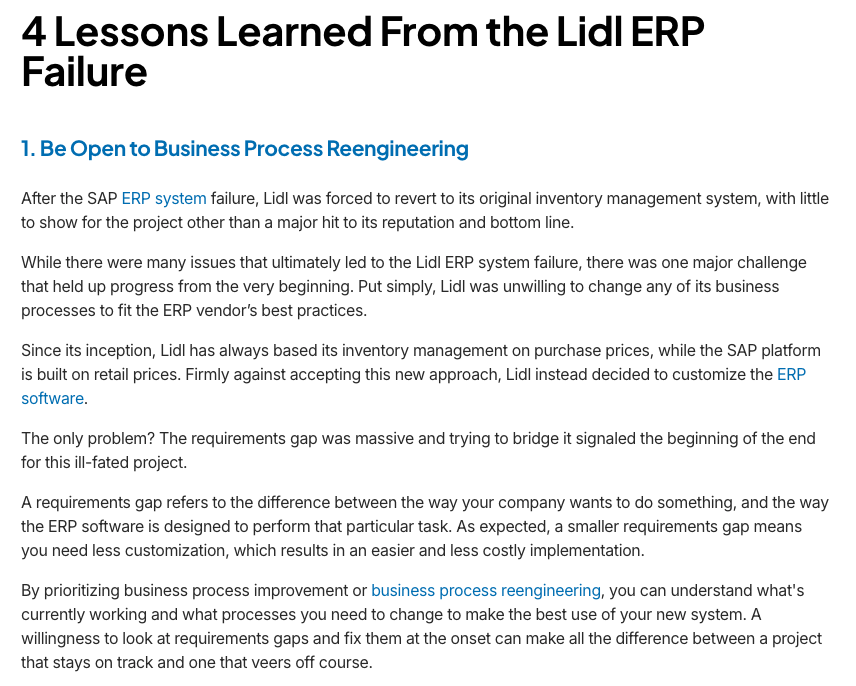
\includegraphics[keepaspectratio,alt={Lessons learned from the Lidl ERP failure -luettelon kohta 1. Be open to business process reengineering.}]{kuviot/lidl-erp.png}}

}

\caption{\label{fig-lidl-erp}ERP-järjestelmän käyttöönotto on lähes
poikkeuksetta myös BPR-projekti\sidenote{\footnotesize https://www.panorama-consulting.com/lidl-erp-failure/}}

\end{figure}%

Davenport ja Short (1990) esittelivät vuonna 1990 viiden vaiheen mallin
(kuva~\ref{fig-davenport-bpr}) prosessien uudelleensuunnitteluun. Malli
ei nykypäivänä välttämättä näytä erityisen kekseliäältä, saati
radikaalilta. Keskeistä mallissa sen julkaisuaikaan oli, ja on tietysti
edelleen, että IT:lle annetaan merkittävä rooli uusia toimintatapoja
suunniteltaessa. Artikkelissa korostetaan, että IT:n todellinen
potentiaali löytyy sen kyvystä mahdollistaa kokonaisvaltaiset
prosessiuudistukset, jotka ylittävät perinteiset osastorajat ja
keskittyvät asiakaslähtöisyyteen.

\begin{figure}

\centering{

\pandocbounded{\includegraphics[keepaspectratio]{index_files/mediabag/kuviot/davenport-bpr.pdf}}

}

\caption{\label{fig-davenport-bpr}Viisivaiheinen malli prosessien
uudelleensuunnitteluun}

\end{figure}%

Aluksi luodaan selkeä visio muutoksen tavoitteille. Priorisoitavien
tavoitteiden tulee olla kunnianhimoisia -- Davenport ja Short (1990)
käyttävät ilmaisua \emph{stretch targets}. BPR-projektia määrittelee,
ettei sillä tavoitella pieniä ja inkrementaalisia uudistuksia.
Seuraavaksi selvitetään, mitä prosesseja uudistuksen tavoitteet
koskevat, ja näistä tunnistetaan kriittiset ja nykyisin pullonkauloja
muodostavat tekijät. Koska uudet prosessit lähtökohtaisesti joka
tapauksessa rakennetaan uudelleen, tulee kriittiset tekijät tuntea sen
vuoksi, että ne voidaan huomioida uusia prosessikulkuja suunniteltaessa
-- ei niinkään siksi, että kehittämiskohteet löydettäisiin ja
määriteltäisiin niiden kautta.

Mikäli projektin laajuutta on tarpeen rajata, työssä on syytä keskittyä
suuren vaikuttavuuden prosesseihin. Esimerkiksi
ERP-järjestelmävetoisessa projektissa täytyy kuitenkin huomata
prosessien kytkeytyminen toisiinsa. Mikäli vaikka tilauskäsittelyn
prosessi rakennetaan uudelleen, tulee varmistua, että muut siihen
kytkeytyvät prosessit saavat vastaavan päivityskäsittelyn prosessien
jatkuvuuden sekä loogisen yhteentoimivuuden varmistamiseksi. Tilanne
vertautuukin tältä osin prosessien ulkoistamiseen, jota käsitellään
myöhemmin.

Edellisessä auttaa, jos nykyiset prosessit tunnetaan ja on dokumentoitu.
Yksinkertaisimmillaan tämä voi tarkoittaa esimerkiksi prosessikarttaa
tai hieman edistyneemmässä tapauksessa prosessisalkkua. Usein kuitenkin
tarvitaan myös tarkempaa prosessidokumentaatiota, kuten BPMN-malleja tai
vastaavia työnkulkukuvauksia. Sen jälkeen tulee analysoida prosessien
nykytilanne. Tässä voidaan tunnistaa vältettävät heikkoudet,
pullonkaulat ja virhealttiit vaiheet. Samalla huomioidaan, onko
prosesseissa on joitain ominaisuuksia, jotka ovat välttämättömiä
säilyttää myös niiden uudessa toteutusmuodossa. Nämä voivat olla
lakisääteisiä tai sääntelyyn liittyviä vaatimuksia ja joissain --
todennäköisesti harvoissa -- tapauksissa joitain kilpailukyvyn kannalta
erityisiä innovaatioita tai kyvykkyyksiä, joista ei haluta luopua.

Uusien prosessien suunnittelussa hyödynnetään asiakastuntemusta,
teknologian tarjoamia mahdollisuuksia ja nojaudutaan mahdollisesti
innovatiivisiinkin ratkaisuihin. BPR-muutosten laajuuden vuoksi
innovointiin ei kuitenkaan tule suhtautua leikkikenttänä, vaan muutosten
tulee olla hyvin suunniteltuja ja mielellään \emph{proof-of-concept}
-tasolla tai pilotoinnilla testattavissa.

\begin{figure}

\centering{

\pandocbounded{\includegraphics[keepaspectratio]{index_files/mediabag/kuviot/teknologia-liiketoiminta.pdf}}

}

\caption{\label{fig-teknologia-liiketoiminta}Teknologiavetoinen ja
liiketoimintavetoinen prosessimuutos}

\end{figure}%

Perustavaa laatua oleva kysymys onkin, millainen rooli teknologialle
muutoshankkeessa annetaan (kuva~\ref{fig-teknologia-liiketoiminta}).
Muutos voidaan toteuttaa teknologiavetoisesti. Tällöin keskitytään
teknologioiden mahdollisuuksiin ja prosessit rakennetaan näiden
mahdollisuuksien muodostaman kivijalan varaan. Toinen vaihtoehto on
suunnitella muutosta liiketoimintalähtöisesti. Tällöin muotoillaan ensin
prosessit ja sen jälkeen etsitään teknologiaratkaisut, jotka tukevat
niiden toteuttamista mahdollisimman hyvin. Ideaalitilanteessa molempia
lähestymistapoja sovelletaan rinnakkain ja jatkuvassa vuoropuhelussa,
eikä organisaation kaikilla toiminta-alueilla ole välttämätöntä soveltaa
samoja periaatetason linjauksia. Joissain toiminnoissa teknologialle
voidaan antaa prosesseja määrittävä rooli ja jossain muualla prosesseja
tukeva rooli. Päätöksenteossa voidaan käyttää esimerkiksi McFarlanin
matriisia (kuva~\ref{fig-mcfarlanin_matriisi}), jonka avulla voidaan
määritellä IT:n rooli eri toiminnoissa tällä hetkellä ja
tulevaisuudessa.

\begin{figure}

\centering{

\pandocbounded{\includegraphics[keepaspectratio]{index_files/mediabag/kuviot/mcfarlanin_matriisi.pdf}}

}

\caption{\label{fig-mcfarlanin_matriisi}McFarlanin matriisi (mukaeltu
Tiirikainen 2008)}

\end{figure}%

Muutosten ollessa suuria, ne todennäköisesti vaikuttavat myös rooleihin
ja tehtävävastuisiin, tietojärjestelmiin ja jopa
organisaatiokulttuuriin. BPR-projekteihin tuleekin aina suhtautua
organisaatiomuutoksina ja huomioida tämä muutoksen läpiviennin
ajankohdassa ja aikataulussa, sidosryhmien osallistamisessa,
koulutuksissa, muutosviestinnässä ja muutosjohtamisessa koko
skaalallaan\sidenote{\footnotesize Laajamittaisia BPR-projekteja saatetaan toteuttaa
  esimerkiksi kesälomakauden aikana, jolloin niiden ajatellaan
  häiritsevän mahdollisimman vähän organisaation operatiivista
  toimintaa. Tällöin uusien toimintatapojen opettelu ja uusien
  järjestelmien häiriöt ovat kuitenkin odottamassa lomalta palaavia
  työntekijöitä.}. Prosessien radikaalin uudistamisen jälkeen toimintaa
seurataan ja arvioidaan KPI- ja muiden prosessimittareiden avulla.

Proctorin (2018) mukaan BPR-projektien epäonnistumiselle tyypillisiä
syitä ovat:

\begin{itemize}
\tightlist
\item
  \textbf{BPR-hanke ei kytkeydy strategisiin tavoitteisiin.} Ilman
  selkeää yhteyttä organisaation strategisiin tavoitteisiin BPR-hankkeet
  voivat menettää suuntansa ja keskittyä epäolennaisiin parannuksiin.
  BPR on liian suuri, kallis ja riskialtis ponnistus toteutettavaksi,
  jos sillä ei lähtökohtaisestikaan ole edellytyksiä saavuttaa
  liiketoiminnan kannalta keskeisiä ja merkittäviä muutoksia.
\item
  \textbf{BPR-hankkeessa korostuu taktisen tason tarkastelu.}
  Keskittyminen ainoastaan päivittäisiin työprosesseihin ilman
  strategisen tason huomioimista voi johtaa pinnallisiin muutoksiin,
  jotka eivät tuota pitkäaikaista arvoa.
\item
  \textbf{BPR-hankkeen rajallinen laajuus ja nykytilanteen suppea
  analyysi.} Pintapuolinen prosessianalyysi ja kapea-alainen
  lähestymistapa voivat estää todellisten ongelmakohtien tunnistamisen
  ja estää merkittävien parannusten toteuttamisen.
\item
  \textbf{Toistuvia malleja ei onnistuta tunnistamaan.} Ilman kykyä
  tunnistaa ja ymmärtää organisaation sisäisiä toistuvia malleja ja
  rakenteita voi olla vaikeaa toteuttaa tehokkaita uudistuksia.
\item
  \textbf{Epäoptimaalinen mahdollisuuksien priorisointi.}
  Mahdollisuuksien priorisointi subjektiivisten tekijöiden perusteella
  voi johtaa resurssien tehottomaan käyttöön ja tärkeiden parannusten
  ohittamiseen.
\item
  \textbf{Passiivinen kehitys ja toteutus.} Uudistusten passiivinen
  lähestymistapa ilman aktiivista suunnittelua ja toteutusta voi estää
  muutosten onnistumisen ja kestävyyden. BPR on radikaali uudistushanke,
  joka edellyttää paitsi nykyisten toimintamallien ja rakenteiden
  purkamista, myös tehokkaan suunnitelman uusien toimintamallien
  rakentamiseksi ja jalkauttamiseksi. Kaikenlaisissa uudistushankkeissa
  onnettomin lopputulema on se, että nykyinen ratkaisu revitään auki,
  mutta tekemisen tahti ja into alkavat hidastua, kun uusi ratkaisu
  tulisi saada toteutettua.
\item
  \textbf{Muutoksenhallinnan puutteet.} BPR on aina huomattava
  organisaatiomuutoshanke ja muutoshankkeiden valitettavan tavallinen
  epäonnistumistekijä on heikko tai epäonnistunut muutosjohtaminen.
  Henkilöstön, prosessien ja teknologian muutosten hallinnan
  laiminlyönti voi johtaa BPR-hankkeen vastustukseen ja estää
  uudistusten onnistumisen.
\item
  \textbf{Teknologian ja prosessien erillinen käsittely.} Teknologian ja
  prosessien erillinen tarkastelu voi estää niiden tehokkaan
  integroinnin ja heikentää uudistusten vaikutusta. BPR-hankkeet
  lähtökohtaisesti pyrkivät uudistamaan toimintatapoja IT-ratkaisujen
  avulla. Sen vuoksi teknologioiden mahdollisuuksien tarkastelua ei saa
  erottaa prosessien tarkastelusta.
\item
  \textbf{Liiallinen luottamus standardimalleihin.} Yleisten mallien ja
  parhaiden käytäntöjen sokea soveltaminen ilman organisaation
  erityispiirteiden huomioimista voi johtaa epäonnistumiseen.
\item
  \textbf{Väärinkäsitykset BPR:n luonteesta.} BPR:n ymmärtäminen
  pelkästään prosessien parantamisena ilman strategista näkökulmaa ja
  IT:n mahdollisuuksien ymmärtämistä voi rajoittaa sen potentiaalia ja
  johtaa epäonnistumiseen.
\end{itemize}

\section{Muutoksenhallinta}\label{muutoksenhallinta}

Liiketoimintaprosessien muutokset ovat lähtökohtaisesti haastavia
muutoshankkeita. Paitsi, että ne muuttavat työnteon tapoja,
suurempimittaiset prosessimuutokset voivat tuoda rooleille uusia
tehtäviä ja vastuualueita, tehdä joistakin tehtävistä tarpeettomia, ja
aiheuttaa muutoksia aina organisaation rakenteissa saakka. Tämä vaatii
koko organisaatiota leikkaavaa uuden opettelua ja vanhoista
toimintatavoista poisoppimista. Prosessimuutosten menestyksekäs
läpivienti edellyttääkin muutosjohtamista.

Systemaattisessa kirjallisuuskatsauksessaan Idogawa ym. (2023)
kartoittivat prosessien kehittämiseen liittyvän muutoksenhallinnan
kriittisiä menestystekijöitä (\emph{Critical Success Factor},
\emph{CSF}) ja muodostivat hypoteeseja aiemmissa tutkimuksissa
argumentoitujen menestystekijöiden välisistä vahvistavista vaikutuksista
sekä vaikutuksista muutoksenhallintaan liiketoimintaprosessien
kehittämisprojekteissa. Jos tuntee CSF-tutkimuksia, löydökset eivät
sinällään ole erityisen yllättäviä: samat menestystekijät vaikuttavat
toistuvan aiheesta riippumatta. Tärkeimmäksi tekijäksi tunnistettiin
projektinhallinta, ja seuraavaksi tärkeimmäksi ylimmän johdon tuki, joka
toimii ratkaisevana välittäjänä muutoksenhallinnan mahdollistamisessa.
Vaikka myös teknologiset kompetenssit todettiin relevanteiksi, oli
niiden merkitys tutkimuksen mukaan toissijaista (Idogawa ym. 2023).

Olipa kyse pienimuotoisesta kehittämisestä tai radikaalimmasta
uudistamisesta, prosessimuutosten läpivienti on syytä toteuttaa
suunnitelmallisesti ja jotain toimivaksi todettua muutosjohtamisen
mallia soveltaen. Tällaisia ovat esimerkiksi Lewinin klassinen
\emph{Unfreeze}-\emph{Change}-\emph{Refreeze} (ks. Keen 1981), Kotterin
kahdeksan vaiheen muutosjohtamismalli ({Kotter ym.} 2007) ja Hiattin
ADKAR-malli (Hiatt 2006). Erilaisille muutosjohtamisen malleille
yhteistä on, että ensin muutoksen tarpeellisuus ja hyödyllisyys
perustellaan, ja muutokselle pyritään luomaan edellytykset. Sitten
muutos toteutetaan ja lopuksi uusi tila vakiinnutetaan.

Prosessimuutosten tapauksessa nykytilan diagnosointi ja analyysi ovat
ehdottoman tärkeitä. Näissä selvitetään, mitä tietoa prosessissa
liikkuu, mitä järjestelmiä sen toteuttamisessa käytetään, mitä rooleja
prosessiin osallistuu ja mitä taitoja näiltä henkilöiltä vaaditaan,
mitkä säännökset prosessia koskevat ja niin edelleen. Kuten edellä
todettiin, mikäli nykytilan prosessit on dokumentoitu, muutoksen
vaikutusten arviointi on huomattavasti helpompaa. Myös
kokonaisarkkitehtuurin tarjoamaa tietoa voidaan tässä käyttää apuna.
Mikäli taas prosessien tuntemus on heikkoa, on muutoksen hallittu
toteuttaminen vaikeaa.

Kun tavoitetilan prosesseja suunnitellaan, tulee huomioida myös niiden
mahdollisesti vaatimat organisaatiomuutokset, laatia viestintä- ja
koulutussuunnitelmat sekä siirtymäskenaariot. Halutaanko uusia
toimintamalleja esimerkiksi pilotoida jossain yksikössä tai jollain
kohdealueella ennen päätöstä laajemmasta jalkauttamisesta? Muutoksen
toteumaa ja vaikutuksia tulee myös jatkuvasti seurata, jotta mahdolliset
virheet ja ongelmat, tai tarpeet hienosäädölle, voidaan tunnistaa ja
niihin reagoida.

Liiketoimintaprosessien muuttaminen ja siihen liittyvä muutoksenhallinta
ovat vaiheineen, haasteineen ja menestystekijöineen hyvin samankaltaisia
projekteja kuin uusien tietojärjestelmien käyttöönotot. Lisäksi nämä
projektit toteutuvatkin usein rinnakkain: tietojärjestelmämuutoksista
voi seurata tarve uudistaa prosesseja tai prosessimuutoksista tarve
uudistaa järjestelmiä.

\section{Prosessien ulkoistaminen}\label{prosessien-ulkoistaminen}

Ulkoistaminen (\emph{outsourcing}) vaikuttaa olevan trendi, joka nousee
toistuvasti pinnalle ja sitten taas katoaa. Tämä on koskenut erityisesti
asiakaspalvelun tehtäviä ja muita tukitoimintoja. Yhdellä hetkellä
näyttää siltä, että lähes kaikki yritykset ulkoistavat esimerkiksi
IT-tukensa prosessit, ja seuraavaksi näitä toimintoja ollaankin jo
siirtämässä takaisin (\emph{insourcing}) yrityksen omaan haltuun.
2000-luvun alussa alkoi yleistyä myös toimintojen ulkoistaminen
ulkomaille (\emph{offshoring}). Monet suuryritykset, kuten IBM ja
General Electric edelläkävijöinä, siirsivät IT-tukea, palvelinkeskuksia
ja jopa ohjelmistokehitystä halvemman työvoiman maihin kuten Intiaan ja
Kiinaan. Samoin tuotantoa ja logistiikkaa ulkoistettiin kansainvälisesti
halvempaa työvoimaa ja mittakaavaetuja tavoitellen. 2010-luvulta alkaen
pilvipalvelujen yleistyessä yhä useammat, jopa liiketoiminnan kannalta
keskeiset IT-järjestelmät, on saatettu siirtää ulkoisten toimijoiden
tarjoamille pilvialustoille.

Ajatuksena tässä on strategia tai johtamismalli, jonka mukaan ainoastaan
ydin- ja kriittiset toiminnot toteutetaan itse ja kaikki muu voidaan
ulkoistaa. Ajatus perustuu Hamelin ja Prahaladin (1990) esittelemään
ydinkyvykkyyden (\emph{Core Competence}) käsitteeseen sekä Williamsonin
(1975) transaktiokustannusteoriaan (\emph{Transaction Cost Theory}).
Yrityksen tulisi keskittyä sellaiseen toimintaan, jossa sillä on vahvaa
osaamista ja jolla se voi saavuttaa kilpailuetua. Jos joku voi toteuttaa
jonkin toiminnon laadukkaammin ja halvemmalla kuin mihin yritys itse
pystyy, miksipä sitä kannattaisi itse tehdä.

McIvor (2000) on esitellyt liiketoimintaprosessien ulkoistamispäätöksiä
ohjaavan viitekehyksen (kuva~\ref{fig-ulkoistuspaatos}). Ensimmäisessä
vaiheessa määritellään, mitä ydintoiminnolla tarkoitetaan. Ne voivat
esimerkiksi olla toimintoja, jotka tuottavat asiakkaille arvoa tai jotka
ovat merkityksellisiä kilpailukyvyn kehittämisen kannalta. Seuraavaksi
tunnistetaan ydintoiminnot ja ei-ydintoiminnot. Tämä toteutetaan
organisaation ylimmän johdon ohjaamana, mutta henkilöstöä laajasti
osallistaen niin hierarkkisesti kuin myös toimialoittain ja
yksikköittäin.

\begin{figure}

\centering{

\pandocbounded{\includegraphics[keepaspectratio]{index_files/mediabag/kuviot/ulkoistuspaatos.pdf}}

}

\caption{\label{fig-ulkoistuspaatos}Viitekehys ulkoistuspäätösten
arviointiin (mukaeltu McIvor 2000)}

\end{figure}%

Kun ydintoiminnot on tunnistettu, arvioidaan valituilla mittareilla
niihin liittyviä organisaation kyvykkyyksiä suhteessa ulkoisiin
toimijoihin. Seuraavaksi pyritään arvioimaan ydintoimintojen
toteuttamisen kokonaiskustannukset, jos ne toteutetaan itse ja toisaalta
jos ne ulkoistettaisiin.

Viitekehyksessä siis oletetaan, että ei-ydintoiminnot lähtökohtaisesti
ulkoistetaan. Poikkeuksena tähän mainitaan ''poliittiset'' syyt, jotka
voivat liittyä toimialan sisäisiin tai ulkoisiin suhteisiin. Esimerkiksi
ammattiliitot ovat joskus voineet heittää kapuloita laajamittaisten
ulkoistussuunnitelmien rattaisiin.

Viimeiseksi arvioidaan, millainen yhteistyö kunkin tunnistetun
potentiaalisen ulkoistuskumppanin kanssa on mahdollista. Onko
esimerkiksi mahdollista solmia strategisia kumppanuuksia, voidaanko
toiminnon ohjaus ja johtaminen säilyttää ulkoistusjärjestelyssä itsellä
(vrt. myöhemmin käsiteltäviin prosessikoreografiaan ja
prosessiorkestraatioon) ja niin edelleen. Mikäli ulkoistusvaihtoehtoon
ei jostain syystä päädytä, vaihtoehtona on edellisten
kyvykkyysanalyysien ohjaamana investoida toimintojen sisäisen
toteutuksen kehittämiseen.

Asiat eivät tietenkään aina ole näin yksinkertaisia. Ensinnäkin
toimintojen onnistunut ulkoistaminen edellyttää, että ydinprosessit,
joita ulkoistettavien toimintojen on tarkoitus tukea, ovat hyvin
hallussa. Ydinprosessien vaatimukset tulee tuntea ja ne tulee pystyä
kommunikoimaan ulkoistuskumppanille niin, että prosessien
yhteentoimivuus ja laatuvaatimukset toteutuvat. Mikäli laatuvaatimusten
varmistaminen vaatii jatkuvaa valvontaa, voi jo se aiheuttaa niin paljon
välillisiä kustannuksia, ja vaatimuksissa epäonnistuminen niin suurta
asiakastyytymättömyyttä tai mainehaittaa, etteivät esimerkiksi
matalampien työvoimakustannusten säästöt maksakaan itseään takaisin.
Ulkoistusrakenteissa myös riskienhallinta muuttuu lähes poikkeuksetta
monimutkaisemmaksi ja aiheuttaa epäsuoria kustannuksia.

\begin{quote}
\textbf{Seuraava erityisesti IT-toimintojen ja niihin liittyvien
prosessien ulkoistamiseen keskittyvä osuus perustuu keskusteluun Ari
Kuusion kanssa. Kuusio on toiminut muun muassa johtaja- ja
päällikkötehtävissä suurissa julkisissa organisaatioissa.}

Kuusio toteaa aluksi, että on tärkeää, että organisaation omat prosessit
tunnetaan ja ne on kuvattu selkeästi. Tämä lähtötilanne mahdollistaa
prosessiulkoistusten tietoperustaisen arvioinnin. Jotta jokin toiminto,
kuten IT-tukipalvelut, voidaan onnistuneesti ulkoistaa, täytyy
organisaation tuntea, mitä prosesseja toimintoon kuuluu, mitkä niistä
toimivat ja mitkä eivät toimi. Samoin täytyy tuntea toiminnan
toteuttamisen nykyiset kustannukset.

Näiden tietojen avulla voidaan mahdollisimman objektiivisesti
määritellä, mitä ulkoistuksella halutaan saavuttaa. Tämä on ensimmäinen
kysymys, joka organisaatiossa tulee esittää, kun ulkoistamista ryhdytään
suunnittelemaan. Oletukseen, että ulkoistaminen aina ja automaattisesti
johtaa matalampiin kustannuksiin ja toiminnan tai palvelujen parempaan
laatuun, kannattaa suhtautua varauksella. Ulkoistamista koskeva
päätöksenteko vaatii aina perusteellisen selvityksen.

Ulkoistamisen kohteet ovat monenlaisia. Tavallisesti ulkoistamisen
mielletään liittyvän johonkin laajaan operatiivisen toiminnan
kokonaisuuteen. Kuusio kuitenkin korostaa, että nykymaailmassa on paljon
toimintoja, jotka jo ovat käytännössä ulkoistettuja, vaikka asiaa ei
välttämättä niin ajateltaisikaan. Monet organisaatiot esimerkiksi
ostavat valmisohjelmistoja, ja talon sisällä tehtävä ohjelmistokehitys
on entistä harvinaisempaa. Toisaalta taas esimerkiksi taloushallinnon
tehtävien siirto ulkoisen toimijan vastuulle on tyypillinen esimerkki
perinteisestä hieman suuremman toimintokokonaisuuden ulkoistamisesta.

Useiden organisaatioiden toimintaan liittyykin tiiviisti joukko
kumppaneita, jotka toteuttavat ulkoistettuja toimintoja.
Ulkoistuskumppanuuksien suunnittelussa voidaan soveltaa esimerkiksi
edellä esitettyä (kuva~\ref{fig-ulkoistuspaatos}) mallia. Asiaa on syytä
tarkastella kokonaisvaltaisesti toiminnan tehokkuuden, tuloksellisuuden
ja toiminnan laadun sekä organisaation kyvykkyyksien kannalta.
Jälkimmäisessä voidaan käyttää apuna esimerkiksi kyvykkyyskarttaa (ks.
kuva~\ref{fig-kyvykkyyskartta}). Pohdintojen tulisi tukea työtä, jossa
muodostetaan strategian mukainen linjaus siitä, ostetaanko jokin
toiminto kumppanilta vai toteutetaanko se itse.

Merkittävänä osakokonaisuutena pohdintaan liittyy tietovirtojen
tarkastelu, koska prosessien ulkoistamiseen liittyy myös
tietosuojakysymyksiä. On ehdottoman tärkeää tietää, mitä tietoja
prosesseissa käsitellään: mitä tietoja niihin menee syötteinä ja mistä
tiedot tulevat, mitä tietoja tai päätöksiä prosessit tuottavat, ja minne
ne prosesseista menevät.

Prosesseja, niihin liittyviä toimintoja tai niiden toteuttamia palveluja
ulkoistettaessa on tavallisesti välttämätöntä siirtää myös niissä
käsiteltävät tiedot oman organisaation ulkopuolelle tai vähintään
mahdollistaa ulkoistuskumppanille pääsy näihin tietoihin. Tässä on
muistettava EU:n yleisen tietosuoja-asetuksen GDPR:n vaatimukset. Tiedon
käsittelyyn liittyviä vastuita ei voida ulkoistaa, vaikka
operatiivisessa mielessä tiedon käsittely olisikin ulkoistettu.

Ajatellaan seuraavassa palvelupistettä\sidenote{\footnotesize Keskitetty
  yhteydenottopiste palvelutuottajan ja käyttäjien välillä. Tyypillinen
  service desk hallinnoi häiriöitä ja palvelupyyntöjä, ja hoitaa myös
  viestinnän käyttäjien kanssa. (ITIL Palvelutuotanto)
  https://www.itsmf.fi/site/assets/files/1931/itil\_2011\_finnish\_glossary\_v1\_01.pdf}
(\emph{Service Desk}), joka on perinteisesti tyypillinen IT-ulkoistuksen
kohde. Kuusion mukaan tarkastelu tulee aloittaa selvittämällä, mitä
nykyisen palvelupisteen tarjoamat palvelut ovat. Palvelukuvaukset
toimivat tässä keskeisessä roolissa. Mikäli palvelut sekä niitä
toteuttavat prosessit on kuvattu hyvin, on ulkoistuksen suunnittelu
helpompaa ja sen lopputulos todennäköisesti laadukkaampi. Jos
ulkoistettavaksi suunniteltuja toimintoja ei tunneta, on hyvin vaikeaa
arvioida, voidaanko ulkoistuksen avulla saavuttaa parempi lopputulos tai
voidaanko nykyinen taso säilyttää pienemmillä kustannuksilla. Mikäli
palvelut tuotetaan vakioidulla tavalla, esimerkiksi ITIL-käytänteiden
tai ISO/IEC 20000\sidenote{\footnotesize https://sales.sfs.fi/fi/index/tuotteet/SFS/ISO/ID2/2/727723.html.stx}
-standardin mukaisesti, on ulkoistusta suunnittelevalla asiakkaalla
oletettavasti varsin hyvä käsitys siitä, mitä hän on ostamassa, ja
vastaavasti palveluntarjoajalla ymmärrys siitä, mitä asiakas haluaa
saada.

Vaikkei organisaatio lopulta lähtisikään laajaan ulkoistukseen,
standardoitujen prosessien ja palvelumuotojen toteuttajiksi on helpompi
löytää osaajia niin talon sisä- kuin ulkopuolelta verrattuna
tilanteeseen, jossa palvelumalli on hyvin omintakeinen.

Prosessien ja palvelujen mittaaminen on oleellista hyvin perusteltujen
ja onnistuneiden ulkoistuspäätösten kannalta. On tärkeää tietää, missä
toiminta on nykyisellään laadukasta, missä olisi kehittämisen varaa ja
mitä kustannuksia palvelut aiheuttavat. Ulkoistaminen ei kuitenkaan saa
olla ongelmien siirtämistä; toimivien prosessien ulkoistaminen on
huomattavasti yksinkertaisempaa ja tuloksellisempaa.

Mittarit palvelevat myös jo toteutettujen ulkoistusten arvioinnissa.
Ulkoistettujen palvelujen mittaaminen kertoo, saadaanko sellaista
palvelua, mistä on sovittu ja toimitetaanko se sovituin ehdoin ja
kustannuksin. Palveluiden laatua ja kustannuksia tulisi mitata
riippumatta siitä, tuotetaanko palvelu itse vai osittain tai kokonaan
kumppanin toimesta. Mikäli ulkoistusratkaisuun päätyneellä
organisaatiolla ei ole lähtötilanteesta verrokkitietoa, eivät mittarit
pysty ilmaisemaan ulkoistuksen vaikutuksia palvelun laatuun ja
kustannuksiin.

Kuusio mainitsee myös, että kun prosesseja ja palveluja toteutetaan
itse, on niiden mukautuvuus ja joustavuus usein parempi kuin
ulkoistuskumppaneiden tuottamissa vaihtoehdoissa. Kuten edellä
todettiin, palveluntuottajien toimintamallit ovat tyypillisesti
vakioituja. Vakioidut toimintamallit mahdollistavat, että asiakkaalle
voidaan tarjota sovittu kiinteä hinta ja että palvelutason toteumaa
voidaan verrata palvelutasosopimukseen (\emph{Service Level Agreement},
\emph{SLA}). Tämä kuitenkin tarkoittaa myös sitä, että asiakas voi
odottaa saavansa ainoastaan sen, mitä sopimuksessa on määritelty. Kaikki
tästä poikkeava aiheuttaa ylimääräisiä kustannuksia -- mikäli
palveluntuottaja ylipäätään suostuu toimittamaan kaikkia tarvittavia
lisäpalveluja.

Tilanne vertautuu suuriin kaupallisiin tietojärjestelmäratkaisuihin.
Niiden käyttäjien tulee mukauttaa prosessinsa yhteensopiviksi
järjestelmiin ohjelmoitujen oletusten kanssa tai vaihtoehtoisesti päätyä
kalliisiin ja vaikeasti ylläpidettäviin räätälöityihin ratkaisuihin sekä
niiden edellyttämiin monimutkaisiin järjestelyihin. Ulkoistusta
mietittäessä onkin tarkasteltava toiminnan vaatimuksia eri
skenaarioissa: mitä kuuluu vakiopalveluun ja mikä on lisämaksullista
palvelua. Tämä tulee ottaa huomioon myös kokonaiskustannuksia
vertailtaessa.

Lopuksi Kuusio korostaa laadukkaiden ulkoistussopimusten merkitystä.
Sopimuksen neuvotteluun ja tekoon täytyy panostaa riittävästi
resursseja. Toinen keskeinen seikka on se, että jos ulkoistukseen
päädytään, tulee varmistaa, että ulkoistavaan organisaatioon jää
yhteyshenkilö, joka huolehtii, että sopimus toteutuu määriteltyjen
ehtojen mukaisesti ja että sitä kehitetään tarvittaessa. Tämä henkilö
toimii siis ulkoistetun toiminnon rajapintana. Rooli voidaan mieltää
ulkoistettujen prosessien paikalliseksi prosessinomistajaksi.

Ulkoistuspäätöksiä tehtäessä on varauduttava myös siihen, että
ulkoistuskumppania voi olla tarpeen vaihtaa tai ulkoistussopimus purkaa.
Sopimus tulee tehdä niin, että ratkaisusta päästään tarvittaessa irti
mahdollisimman sujuvasti. Ulkoistuksen lisäksi puhutaankin palvelujen
takaisinotosta omaan organisaatioon (\emph{insourcing}).
Insourcing-tarkasteluun pätevät monet samat kysymykset kuin ulkoistuksia
pohdittaessa. Molemmissa tapauksissa esimerkiksi prosessien ja
palvelujen kuvaaminen, vakiointi ja mittaaminen sekä laadukkaat
sopimukset ovat keskeisessä roolissa.
\end{quote}

Organisaation ulkoistaessa joitain liiketoimintaprosessejaan tai osia
prosesseista, on prosessien suunnittelussa silloin kyse oikeastaan
prosessiorkestraatiosta tai -koreografiasta, jossa keskeistä on
prosessien yhteentoimivuus ja rajapinnat. Tätä teemaa käsitellään
myöhemmin.

\bookmarksetup{startatroot}

\chapter{Prosessiarkkitehtuuri}\label{prosessiarkkitehtuuri}

Prosessiarkkitehtuuri määritellään kirjallisuudessa tavallisesti
liiketoimintaprosessien ja niiden keskinäisten riippuvuuksien
kokonaisuudeksi (Dijkman ym. 2011; Eid-Sabbagh ym. 2012), joka tarjoaa
organisaatioille välineen suurien prosessikokonaisuuksien
hallitsemiseksi (Gonzalez-Lopez ja Bustos 2019). Suuremmissa
organisaatioissa prosessien määrä voi helposti liikkua useissa
kymmenissä tai jopa sadoissa.

Prosessiarkkitehtuurin voidaan katsoa olevan
prosessiorganisaatiomuotoisen toiminnan mahdollistaja ja välttämätön
perusta prosessijohtamiselle. Prosessiarkkitehtuurin laadinta alkaa
prosessien tunnistamisella ja ymmärtämisellä. Ensimmäiseksi
organisaation toimintalogiikka tai ansaintamalli jäsennellään
prosesseiksi ja niiden muodostamaksi verkostoksi esimerkiksi
prosessihierarkian muotoon. Apuvälineenä voidaan käyttää vaikkapa edellä
esiteltyä Business Model Canvasia.

\section{Prosessiarkkitehtuurin
muodostaminen}\label{prosessiarkkitehtuurin-muodostaminen}

Dijkman ym. (2011) ovat koonneet lähestymistapoja prosessiarkkitehtuurin
jäsentämiseksi. Näistä ensimmäinen (\emph{Goal-based}) perustuu
liiketoiminnan tavoitteisiin ja tavoitteiden suhteisiin, ja prosessit
tunnistetaan ja johdetaan niiden perusteella. Tavoitelähtöinen tapa
mahdollistaa prosessien tarvelähtöisen arvioinnin: miksi jotain
prosessia tarvitaan vai tarvitaanko sitä ollenkaan.

Toimintalähtöisessä (\emph{Action-based}) lähestymistavassa
tarkastellaan liiketoimintoja, niiden tehtäviä ja toimintojen
rakenteita. Lähestymistapa perustuu \emph{Business Action Theory}
-malliin (Gonzalez-Lopez ja Bustos 2019), jossa oletuksena on, että
liiketoiminta ei ole ainoastaan teknistä ja mekaanista suorittamista
vaan inhimillistä vuorovaikutusta, jossa toimijat pyrkivät saavuttamaan
päämääriä yhteistyön, viestinnän ja merkityksien kautta. Malli
perustuukin Habermasin kommunikatiivisen toiminnan teoriaan, jonka
mukaan toimijat ilmaisevat intentioita, vaihtavat tietoa ja
neuvottelevat. Toimintalähtöinen lähestymistapa voi auttaa tunnistamaan
merkityksiä, sääntöjä ja rooleja liiketoimintaprosessien taustalla.
Käytännössä kyse on siitä, että prosessit pyritään tunnistamaan
organisaation ja sen aktoreiden toimintaa havainnoimalla. Lähestymistapa
on jokseenkin ''akateeminen'', ja sen tuloksellinen soveltaminen
vaatinee oikeanlaista mielenlaatua.

Oliolähtöisessä (\emph{Object-based}) tavassa liiketoiminta jäsennetään
ensin ohjelmistokehityksestä tutun oliomallin muotoon esimerkiksi UML:n
luokkakaaviota käyttäen. Dijkman ym. (2011) esittävät kolme
liiketoimintaolion tyyppiä: pysyvät oliot (\emph{Permanent Objects}),
tapausoliot (\emph{Case Objects}) ja muut oliot (\emph{Other Objects}).
Pysyvät oliot ovat kohteita, joiden elinkaari on pitkä: tyypillisenä
esimerkkinä vaikkapa asiakas. Prosessit tunnistetaan tarkastelemalla
mitä asioita tai toimintoja pysyviin olioihin liittyy ja edelleen, millä
nämä asiat ja toiminnot toteutetaan. Tapausoliot ohjaavat prosessien
suorittamista ja siten prosessit ovat suoraan tunnistettavissa niiden
perusteella (kuva~\ref{fig-olio-suunnittelu}).

\begin{figure}

\centering{

\pandocbounded{\includegraphics[keepaspectratio]{index_files/mediabag/kuviot/olio-suunnittelu.pdf}}

}

\caption{\label{fig-olio-suunnittelu}Prosessiarkkitehtuurin
oliolähtöinen suunnittelu}

\end{figure}%

Referenssimallitapa (\emph{Reference Model based}) soveltuu
käytettäväksi silloin, kun organisaatiolla on jo olemassa jonkinlainen
prosessikartta. Kartta otetaan tarkastelun lähtökohdaksi ja
prosessiarkkitehtuuri muokataan sen perusteella. Tässä toimintatavassa
voidaan hyödyntää myös toimialakohtaisia yleisiä viite- ja
referenssiarkkitehtuurikuvauksia. Seuraavassa kuviossa
(kuva~\ref{fig-tem-viite}) on työn löytymisen prosessit, kuten ne on
esitetty Työvoimapalveluiden viitearkkitehtuurissa\sidenote{\footnotesize https://tem.fi/tyovoimapalveluiden-viitearkkitehtuuri}.
Referenssimalli tarjoaa raamit sille, mitä prosesseja ja palveluja
toimialan viranomaisten tulee toteuttaa. Esimerkkejä yksityisen sektorin
referenssimalleista ovat telekommunikaatioalan viitearkkitehtuuri TM
Forum Frameworx\sidenote{\footnotesize https://www.tmforum.org/frameworx-evolution/},
joka sisältää muun muassa eTOM-viitekehyksen (\emph{enhanced Telecom
Operations Map}) sekä pankki- ja finanssialan Banking Industry
Architecture Network (BIAN)\sidenote{\footnotesize https://bian.org/}.

\begin{figure}

\centering{

\pandocbounded{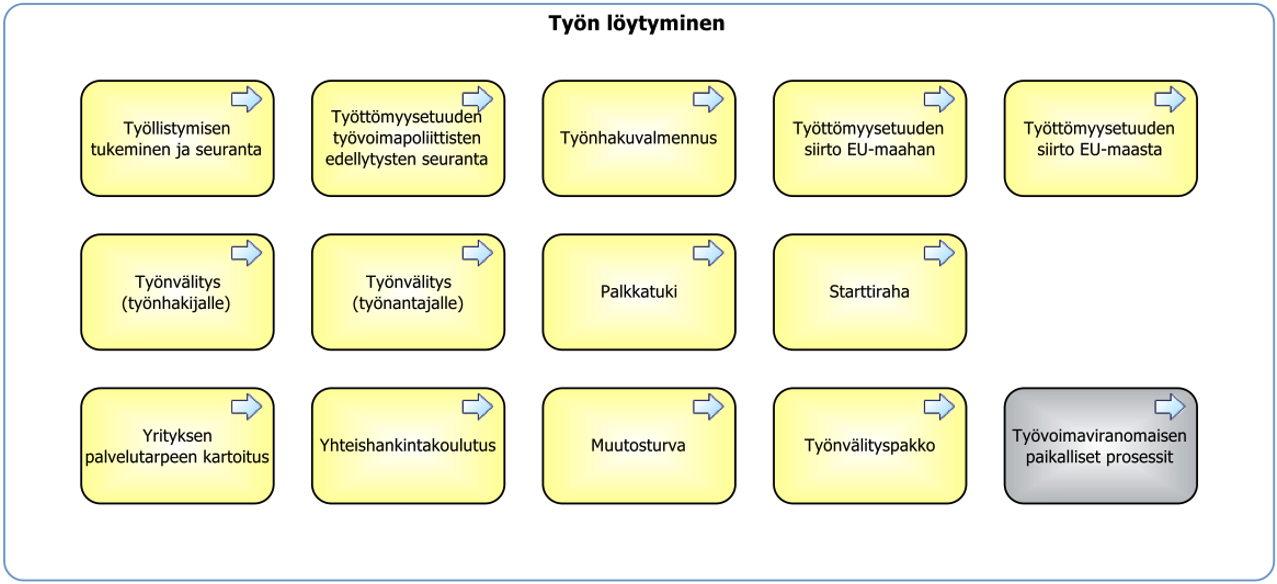
\includegraphics[keepaspectratio]{kuviot/tem-viite.png}}

}

\caption{\label{fig-tem-viite}Työn löytymisen prosessit --
Työvoimapalveluiden viitearkkitehtuuri työvoimaviranomaisille}

\end{figure}%

Toimintolähtöisessä lähestymistavassa (\emph{Function-based})
hyödynnetään toimintahierarkiaa, jolla liiketoiminnot jaetaan
yksityiskohtaisempiin alatoimintoihin. Tämän jälkeen
toimintohierarkiasta tunnistetaan prosessikandidaatit
(kuva~\ref{fig-toim-hier}). Toimintolähtöisen tavan hyödyksi voidaan
mainita se, että sen avulla ajatukset on helpompi keskittää
\emph{mitä}-kysymyksiin, kun taas prosesseista puhumisella on taipumus
johdattaa ajattelu suoraan \emph{miten}-kysymyksiin. Prosessikulkujen
suunnittelu ei vielä prosesseja tunnistettaessa ole ajankohtaista.

\begin{figure}

\centering{

\pandocbounded{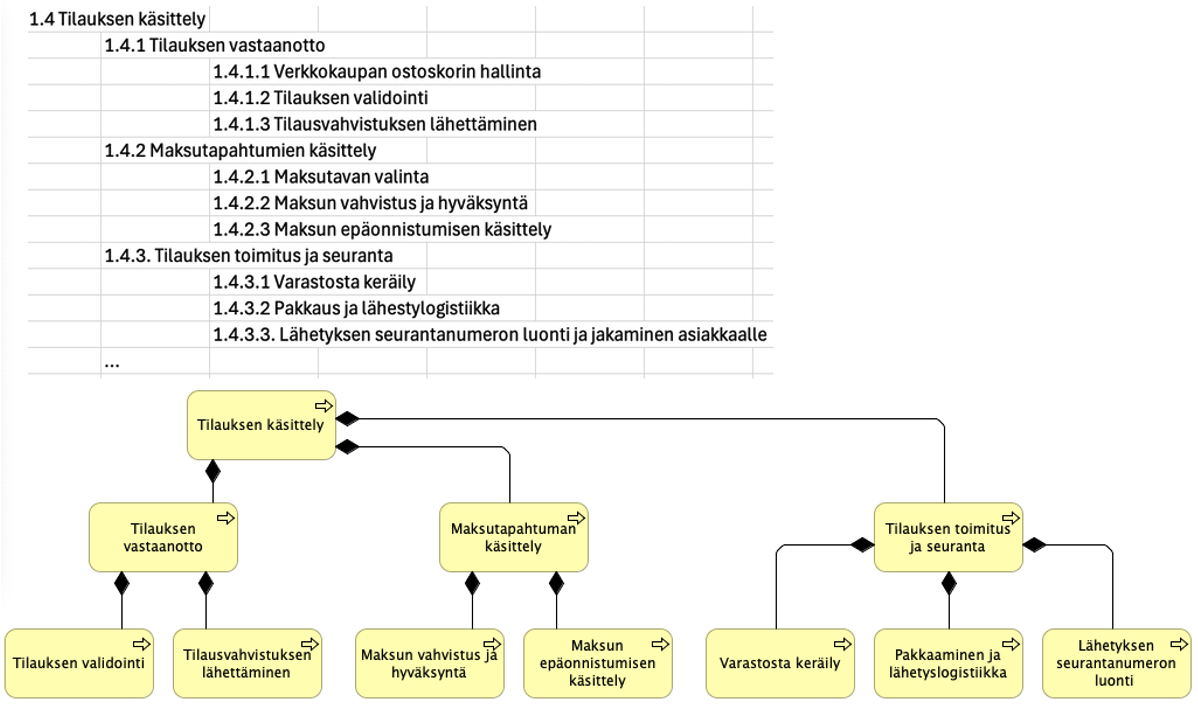
\includegraphics[keepaspectratio]{kuviot/toim-hier.png}}

}

\caption{\label{fig-toim-hier}Toimintohierarkian jalostaminen
prosesseiksi ja aliprosesseiksi}

\end{figure}%

Prosessien tunnistamisen ja prosessikartan laadinnan lisäksi
prosessiarkkitehtuurin muodostamiseen liittyvä tehtävä on prosessin
omistajien tunnistaminen sekä prosessijohtamisen mallista sopiminen.
Ennen prosessiarkkitehtuurin kuvaamisen aloittamista tulee myös sopia
kuvaustavoista: millä notaatiolla tai notaation osajoukolla ja
välineillä prosessit dokumentoidaan, kuka ne dokumentoi, missä kuvauksia
säilytetään, kuinka niitä versioidaan ja miten niiden ajantasaisuus
varmistetaan.

\section{Liiketoimintaprosessit osana
kokonaisarkkitehtuuria}\label{liiketoimintaprosessit-osana-kokonaisarkkitehtuuria}

Kokonaisarkkitehtuurimenetelmät (\emph{Enterprise Architecture}), kuten
hallitseva kansainvälinen standardi TOGAF\sidenote{\footnotesize https://www.opengroup.org/togaf}
(\emph{The Open Group Architecture Framework}) tai Suomen
julkishallinnon käyttöön kehitetty Suomi.fi
-kokonaisarkkitehtuurikehys\sidenote{\footnotesize https://kehittajille.suomi.fi/palvelut/kokonaisarkkitehtuuri/kokonaisarkkitehtuurikehys},
ohjaavat tarkastelemaan laajoja ja monimutkaisia organisaatioita
helpommin hallittavina osakokonaisuuksina ja kokonaisuuksien välisinä
suhteina. Molemmat mainituista menetelmistä esittävät organisaation
tarkastelun näkökulmiksi liiketoiminnan, tiedon (datan ja informaation),
tietojärjestelmät sekä teknologiat. Oleellista KA-menetelmissä on, että
eri näkökulmiin tai arkkitehtuureihin kuuluvien kohteiden väliset
suhteet ja riippuvuudet tehdään näkyviksi.

Kokonaisarkkitehtuurissa voitaisiin olla kiinnostuneita esimerkiksi
yrityksen arvolupauksesta ja siihen liittyvinä kohteina niistä
liiketoimintaprosesseista, joilla tätä lupausta pyritään toteuttamaan.
Näiden prosessien suorittaminen on todennäköisesti riippuvaista joistain
tietojärjestelmistä, jotka tuottavat, käsittelevät ja tallentavat
prosessissa liikkuvaa tietoa. Tietojärjestelmät tarvitsevat toimiakseen
teknologia-alustoja. Näiden kokonaisarkkitehtuurin komponenttien
(arvolupaus, prosessit, tiedot, tietojärjestelmät, teknologia-alustat)
ja niiden välisten suhteiden kautta voidaan hahmottaa organisaation
rakennetta ja toimintaa kokonaisuutena, eli toisin sanoen muodostaa
käsitys kokonaisarkkitehtuurista.

Tarkastelemalla organisaation strategisia tavoitteita tai niihin
liittyviä arvolupauksia, liiketoimintaprosesseja tai niiden
virtausnopeuksia, tietojärjestelmiä, niiden vasteaikoja tai
käytettävyyttä toisistaan irrallaan, ei ole mahdollista ymmärtää ja
arvioida organisaatiota ja sen toimintaa kokonaisuutena, saati tunnistaa
siitä täsmällisiä kehittämiskohteita. Yksittäisen kohteen muuttaminen
ilman ymmärrystä muutoksen heijastus- ja kokonaisvaikutuksista johtaa
harvoin hyvään lopputulemaan.

Vaikka prosessien hallintaa ja kehittämistä voidaan tietysti tehdä ilman
kokonaisarkkitehtuurimenetelmien tukeakin, tarjoavat ne prosessityölle
kontekstin, joka puolestaan mahdollistaa valistuneemman päätöksenteon ja
kehittämisresurssien kohdentamisen. Kokonaisarkkitehtuurin kannalta
edellä käsitelty prosessiarkkitehtuuri on yksi sen osa-alueista tai
oikeastaan yksi, joskin varsin oleellinen, liiketoiminta-arkkitehtuurin
osa-alue.

BPMN-mallinnuskieltä myöhemmin käsiteltäessä tarkastellaan, kuinka sen
avulla voidaan kuvata viestivirtoja, -varastoja ja -järjestelmiä osana
prosessimalleja. Prosessimallien pääasiallinen tarkoitus on kuitenkin
esittää prosessin kulku. Vaikka automatisoitavissa prosessikuluissa
tietovirrat täytyykin mallintaa yksityiskohtaisesti -- muuttujien ja
tietotyyppien tasolla -- ja prosessien tulee pystyä teknisesti
kytkeytymään tietojärjestelmien rajapintoihin, eivät prosesseja
ympäröivät tietovarastot ja järjestelmät ole varsinaisesti
prosessiasiantuntijoiden työmaata. Niitä, kuten myös esimerkiksi
prosessiin liittyviä tietoturvallisuusvaatimuksia, koskevan informaation
tulee kuitenkin olla prosessikehittäjien saatavilla silloin, kun sitä
tarvitaan. Tällaista tietoa kokonaisarkkitehdit voivat tarjota
prosessityön tueksi.

\subsection{Prosessit TOGAF-menetelmässä ja
ArchiMate-mallinnuskielellä}\label{prosessit-togaf-menetelmuxe4ssuxe4-ja-archimate-mallinnuskielelluxe4}

TOGAF-menetelmän kattamien tietosisältöjen metamalli (\emph{Enterprise
Metamodel}\sidenote{\footnotesize https://pubs.opengroup.org/togaf-standard/architecture-content/chap02.html\#tag\_02\_03})
esittää käsitteet, joista organisaation kokonaisarkkitehtuuri muodostuu.
Mallissa liiketoimintaprosessi liittyy välittömillä suhteilla seuraaviin
käsitteisiin: organisaatioyksikkö (\emph{Organization Unit}), rooli
(\emph{Role}), liiketoimintakyvykkyys (\emph{Business Capability}),
arvovirta (\emph{Value Stream}), toiminto (\emph{Function}), tapahtuma
(\emph{Event}), kontrolli (\emph{Control}), liiketoimintatieto
(\emph{Business Information}) sekä liiketoimintapalvelu (\emph{Business
Service}). Data, sovellukset ja teknologiat kytkeytyvät metamallissa
prosessiin edellisten kautta.

Liiketoimintaprosesseilla on siis KA-malleissa kirjaimellisestikin
keskeinen asema -- ja miksipä ei olisi. Prosessien avulla toteutetaan
asiakkaille tarjottavat tuotteet ja palvelut. Prosessien toteuttamisen
tukena käytetään tietojärjestelmiä ja sovelluksia, joten prosessit myös
määrittävät IT-ratkaisuja koskevat vaatimukset. Prosesseissa käsitellään
tietoa, joka tapauksesta riippuen voi pitää sisällään esimerkiksi
henkilötietoja tai liiketoiminnan kannalta kriittistä tai salassa
pidettävää tietoa, ja niin edelleen. Voidaan ajatella, että kaikki
organisaatioiden kokonaisvaltaisen kehittämisen kysymykset lähtevät
liikkeelle prosesseista tai ne ainakin jossain vaiheessa päätyvät
prosesseihin.

TOGAF:iin kuuluva arkkitehtuurin kehittämismenetelmä (\emph{Architecture
Development Method}\sidenote{\footnotesize https://pubs.opengroup.org/togaf-standard/adm/})
ohjaakin arkkitehtuurimuutoksia tehtäessä kiinnittämään ensimmäisenä
huomion liiketoimintanäkökulman (\emph{Business Architecture})
sisältöihin, niiden vaatimuksiin ja niille asetettavaan tavoitetilaan.

Edellä todettiin, että BPMN-mallit on tarkoitettu kuvaamaan prosessin
yksityiskohtaista työnkulkua, mutta niiden mahdollisuudet esittää
prosessin kontekstia ja toimintaympäristöä ovat rajalliset. KA-kuvaukset
pystyvät sen sijaan esittämään organisaation loogisen rakenteen ja
ympäristön kokonaisuudessaan, mutta tyypillisesti varsin karkealla
tarkkuustasolla.

Monet ammattilaisten suosimat mallinnusvälineet tukevat useiden
mallinnuskielten käyttöä rinnakkain, kuten ArchiMatea\sidenote{\footnotesize https://www.opengroup.org/archimate-forum/archimate-overview}
varsinaisten KA-kuvausten tuottamiseen, UML-kieltä tarkempien
ohjelmistoarkkitehtuurien suunnitteluun ja BPMN-kieltä prosessikulkujen
kuvaamiseen. Tällaisten välineiden avulla voidaan tarkastella
esimerkiksi ArchiMatella tuotettua prosessi- (kuva~\ref{fig-am-esim7})
tai kyvykkyyskarttaa (vrt. kuva~\ref{fig-kyvykkyyskartta}) ensin
yleisellä tasolla, jotta nähdään vaikkapa prosessien suhde
liiketoiminnan strategisiin tavoitteisiin tai järjestelmärajapintoihin
kokonaisuudessaan. Tämän jälkeen voidaan porautua tutkimaan tarkemmin
haluttuja prosessikulkuja BPMN-mallien muodossa.

ArchiMate 3.2 -kielen sallimat suhteet liiketoimintaprosessin ja muiden
kohteiden välille on koottu seuraavaan kuvioon
(kuva~\ref{fig-am-bp-suhteet}). Kohteet on värikoodattu näkökulmittain:
keltainen esittää liiketoiminta-arkkitehtuurin (\emph{Business})
elementtejä, vaaleansininen sovelluksiin (\emph{Application}) liittyviä
elementtejä, vihreä teknologiaa (\emph{Technology}) ja niin edelleen.

\begin{figure}

\centering{

\pandocbounded{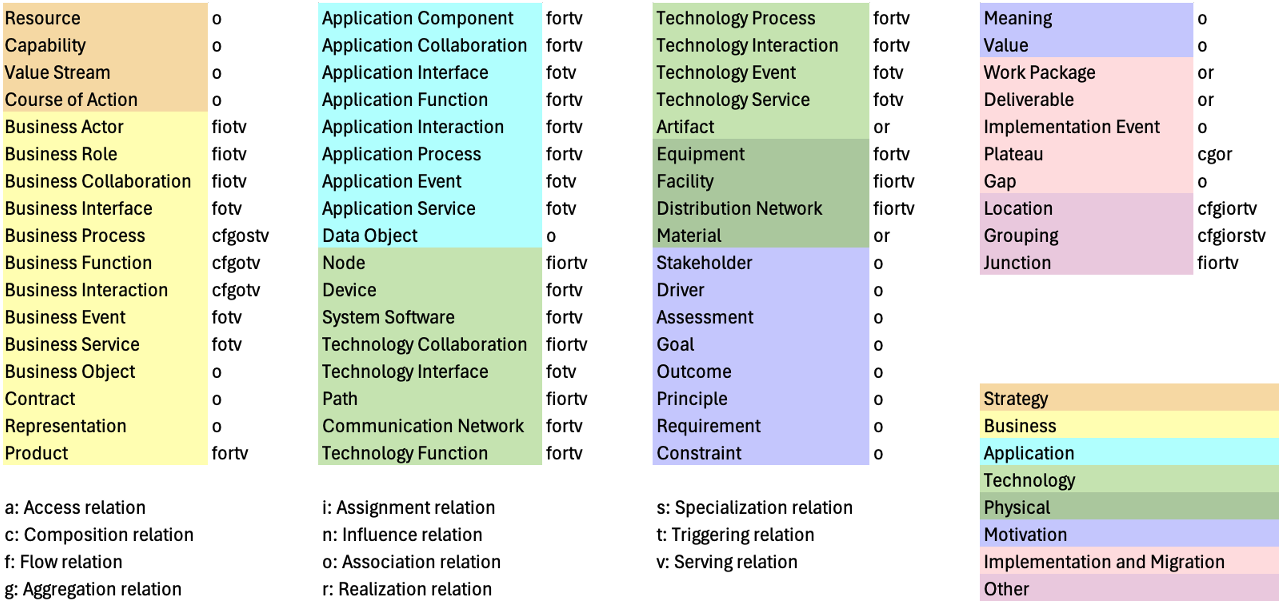
\includegraphics[keepaspectratio]{kuviot/am-bp-suhteet.png}}

}

\caption{\label{fig-am-bp-suhteet}ArchiMate-mallinnuskielen sallimat
suhteet prosessin (Business Process) ja muiden elementtien välille}

\end{figure}%

Esimerkiksi \emph{Business Role} (käytännössä siis tehtävänimike ja muu
henkilöön tai organisaatioyksikköön liittyvä toiminnallinen rooli) voi
liittyä prosessiin seuraavilla suhteilla: \emph{Flow},
\emph{Assignment}, \emph{Association}, \emph{Triggering} tai
\emph{Serving}. Flow ilmaisee jonkin hyödykkeen tai resurssin, kuten
informaation, materiaalin tai rahan, siirtymistä kohteiden välillä.
Assignment esittää vastuun tai suoritusvelvollisuuden allokointia.
Esimerkiksi siis niin, että jokin rooli on osoitettu tietyn prosessin
toteuttajaksi ja toinen rooli prosessin omistajaksi. Triggering kuvaa
kohteiden välistä ajallista tai kausaalista suhdetta; tässä yhteydessä
esimerkiksi sitä, että rooli käynnistää prosessin suorittamisen. Serving
nimensä mukaisesti ilmaisee, että prosessi palvelee jotain roolia tai
rooli palvelee prosessia, riippuen suhteen esityssuunnasta.

Prosessin ja sovelluksen (\emph{Application Component}) välille
ArchiMate sallii muuten samat suhteet kuin rooliin, mutta järjestelmää
ei voida liittää liiketoimintaprosessiin Assignment-suhteella. Sen
sijaan voidaan käyttää \emph{Realization}-suhdetta, jolla ilmaistaan,
että sovellus toteuttaa prosessin tai osallistuu sen toteuttamiseen.
Sovellus voidaan kuitenkin liittää Assignment-suhteella
\emph{Application Process} -tyyppiseen elementtiin, jolla kuvataan
sovelluksen sisäisen toimintalogiikan prosesseja tai automatisoituja
prosesseja.

Kokonaisarkkitehtuurissa ollaan siis erityisesti kiinnostuneita siitä,
kuinka asiat liittyvät toisiinsa ja millaisen kokonaisuuden ne
muodostavat. Sen sijaan prosessikulkujen yksityiskohtaiseen esittämiseen
ArchiMate ei juuri sovellu, eikä sitä ole siihen tehtävään
tarkoitettukaan.

Kokonaisarkkitehtuurimalleissa prosessit esitetään tavallisesti
ainoastaan prosessin nimen tarkkuudella -- ei työnkulkuina. Seuraavassa
esimerkissä (kuva~\ref{fig-am-esim1}) on kolme kohdetta ja niiden
väliset suhteet. Application Component -elementillä kuvattu
\emph{Järjestelmä} tukee Serving-suhteen kautta \emph{Prosessin}
suorittamista. Realization-suhde ilmaisee, että tämä prosessi toteuttaa
liiketoimintapalvelun \emph{Palvelu}.

\begin{figure}

\centering{

\pandocbounded{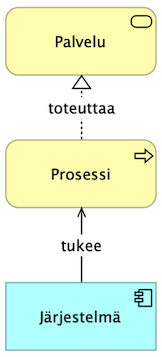
\includegraphics[keepaspectratio]{kuviot/am-esim1.png}}

}

\caption{\label{fig-am-esim1}ArchiMaten prosessi-, palvelu- ja
sovelluselementit}

\end{figure}%

Seuraava kuvio (kuva~\ref{fig-am-esim2}) esittää laskunkäsittelyn
prosessin vaiheittain. Prosessikulun käynnistää \emph{Lasku saapuu},
joka on Business Event -tyyppinen tapahtuma. Sillä voidaan ilmaista
liiketoiminnan kannalta relevanttia tilan muutosta, jollaisena laskun
vastaanottamista voidaan toki pitää. Vastaava prosessikulku BPMN:llä
esitettynä käynnistyisi \emph{Message Start Event} -tapahtumalla, johon
palataan myöhemmin. Toinen merkittävämpi ero, ja ilmeinen puute
ArchiMaten mahdollisuuksissa kuvata prosessikulkuja, on se, että siinä
ei ole tehtävätyyppistä (\emph{Task} tai \emph{Activity}) elementtiä.
Siksi laskunkäsittelyprosessin jokainen vaihe täytyy mallintaa omaksi
prosessikseen. Näin tietysti voidaan tehdä ja ehkä vaikkapa
\emph{Hyväksy lasku} -tehtävä voi joskus olla hyödyllistäkin hahmottaa
ja kuvata omana prosessinaan tai aliprosessinaan.

Käytettäessä ArchiMatea prosessien kuvaamisen tekniikkana ajaudutaan
kuitenkin nopeasti tilanteeseen, jossa prosesseina esitettyjä tehtäviä
kertyy mallikantaan valtava määrä, ja prosessisalkun hallinta on
vaarassa ruuhkautua. Tästäkin syystä prosessikulut on järkevämpää kuvata
siihen nimenomaisesti tarkoitetuilla mallinnuskielillä, kuten BPMN:lla.

Yksi esimerkkikuviosta huomattava ArchiMaten etu liittyy mahdollisuuteen
liittää tietojärjestelmiä ja järjestelmäpalveluja suorittamisen
vaiheisiin tarkemmalla tasolla kuin BPMN-malleissa.

\begin{figure}

\centering{

\pandocbounded{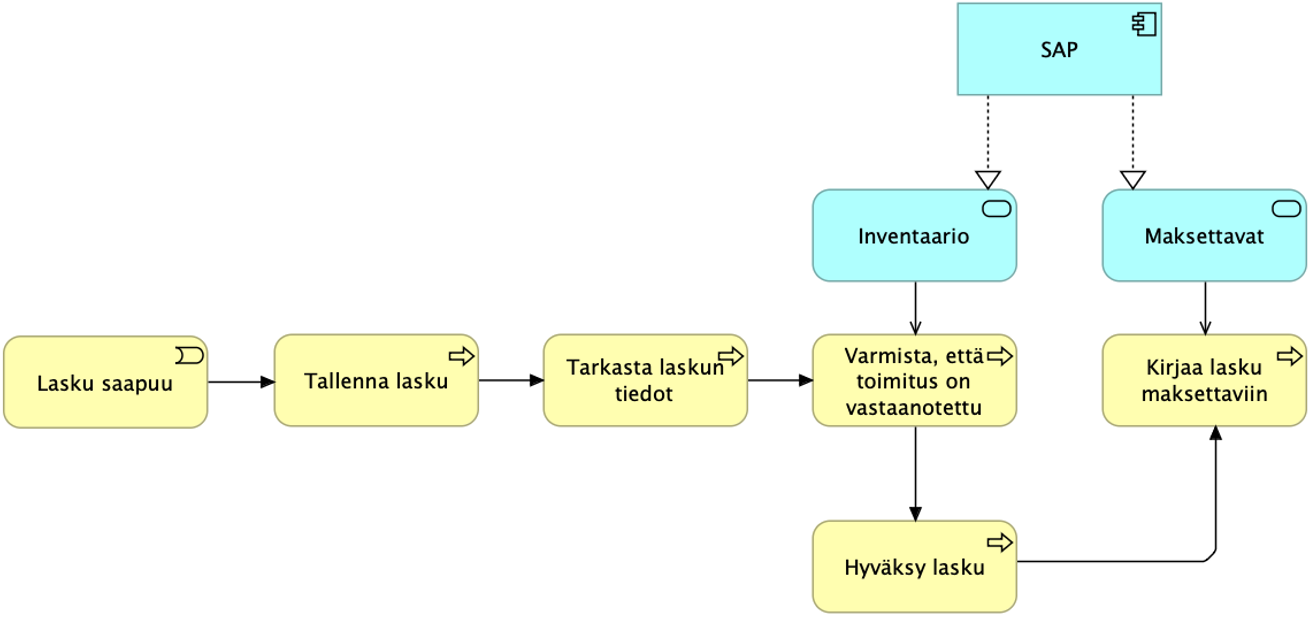
\includegraphics[keepaspectratio]{kuviot/am-esim2.png}}

}

\caption{\label{fig-am-esim2}Laskunkäsittelyn prosessi ArchiMatella
esitettynä}

\end{figure}%

ArchiMaten \emph{Business Actor}- ja \emph{Business Role} -elementtejä
voidaan käyttää esitettäessä prosessiin liittyviä toimijoita ja
sidosryhmiä. Seuraavassa esimerkissä (kuva~\ref{fig-am-esim3})
prosessiin on liitetty kaksi aktoria (\emph{Omistaja} ja \emph{Asiakas})
ja yksi rooli (\emph{Toteuttaja}). Tällaiseen informaatioon tukeutuen
voitaisiin helposti löytää esimerkiksi prosessit, joilla ei ole nimettyä
omistajaa tai tarkastella sitä, millä prosesseilla tiettyä kriittistä
asiakasryhmää palvellaan.

\begin{figure}

\centering{

\pandocbounded{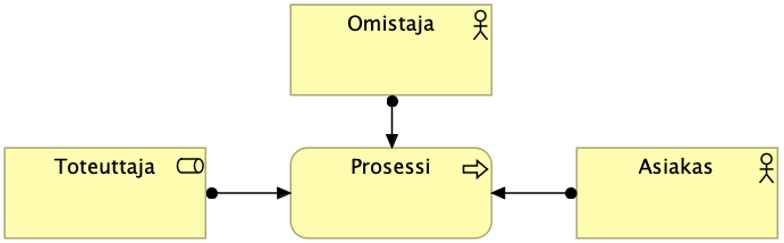
\includegraphics[keepaspectratio]{kuviot/am-esim3.png}}

}

\caption{\label{fig-am-esim3}Business Actor- ja Business Role
-elementtejä liitettynä prosessiin Assignment-suhteella}

\end{figure}%

ArchiMate-malleissa voidaan aktoreiden ja roolien avulla myös jäljitellä
BPMN:n uima-altaita ja -ratoja. Näin toimittaessa malli voi olla
helpommin luettava, eikä se menetä mitään informaatiosisällöstään
(kuva~\ref{fig-am-esim4}).

\begin{figure}

\centering{

\pandocbounded{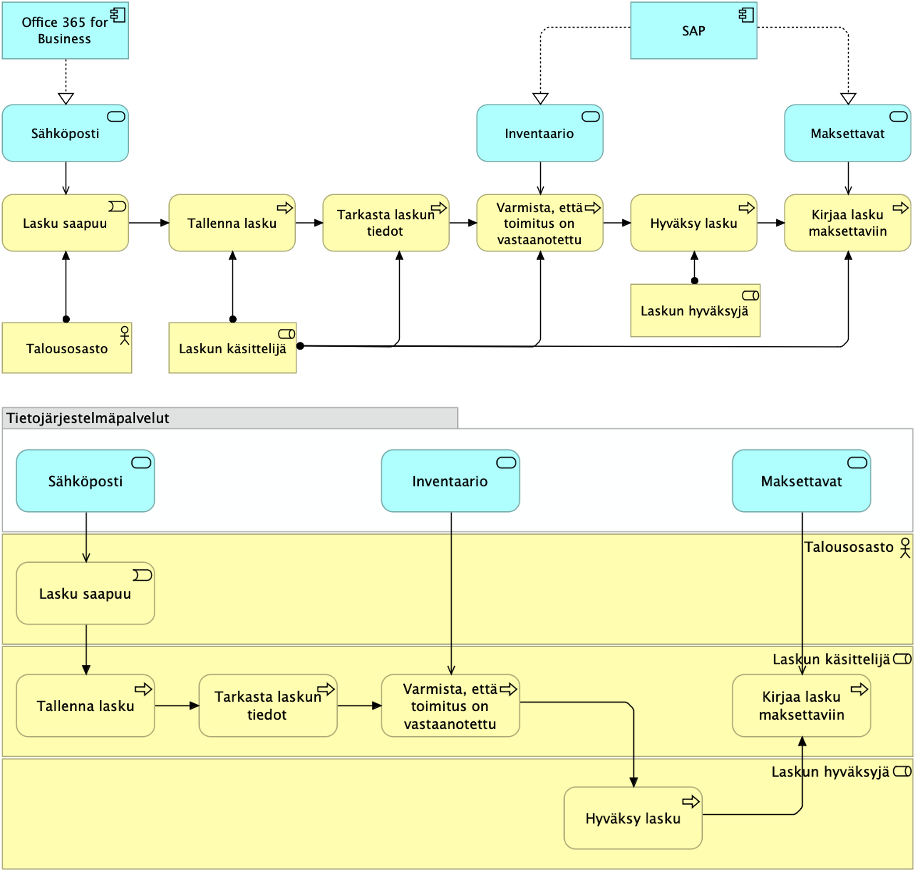
\includegraphics[keepaspectratio]{kuviot/am-esim4.png}}

}

\caption{\label{fig-am-esim4}Organisaatio- ja rooliuimaratoja
ArchiMatella}

\end{figure}%

ArchiMaten \emph{Junction}-elementillä on mahdollista kuvata hieman
tarkemmin prosessikulun logiikkaa. Junction voi olla tyypiltään AND
(täytetty musta ympyrä) tai OR (täyttämätön ympyrä). Niitä voidaan
käyttää kuten BPMN:n Parallel Gateway- tai Exclusive Gateway -portteja
(kuva~\ref{fig-am-esim5}).

\begin{figure}

\centering{

\pandocbounded{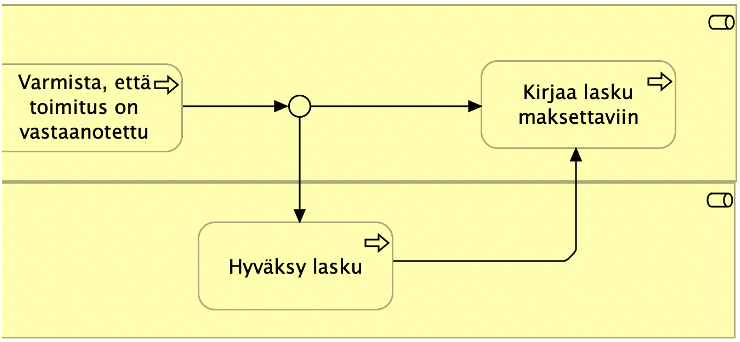
\includegraphics[keepaspectratio]{kuviot/am-esim5.png}}

}

\caption{\label{fig-am-esim5}ArchiMaten OR Junction}

\end{figure}%

Prosessiin kuuluvat aliprosessit voidaan esittää koostumista ilmaisevan
suhteen (\emph{Composition} ja \emph{Aggregation}) avulla
(kuva~\ref{fig-am-esim6}).

\begin{figure}

\centering{

\pandocbounded{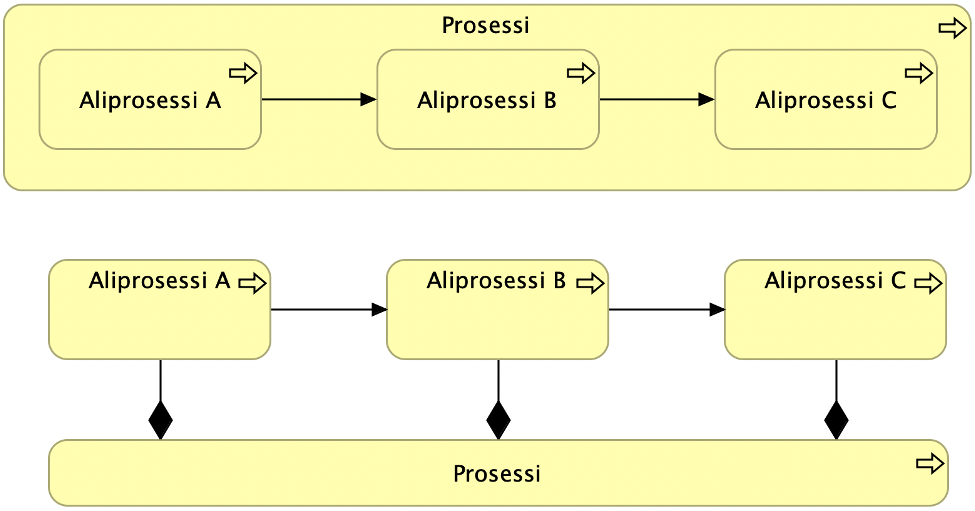
\includegraphics[keepaspectratio]{kuviot/am-esim6.png}}

}

\caption{\label{fig-am-esim6}Prosessi ja sen aliprosessit
nested-rakenteella (ylempi) ja Composition-suhteella (alempi)
esitettyinä}

\end{figure}%

Liiketoimintaprosessien hallinnan kannalta
kokonaisarkkitehtuuri-informaation merkittävin hyöty perustuu sen
kattamien kohteiden ja näkökulmien monipuolisuuteen sekä kykyyn esittää
niiden välisiä suhteita ja riippuvuuksia. Esimerkiksi prosessikarttaa
voitaisiin rikastaa riippuvuussuhteiden kautta muodostuvalla
informaatiolla (kuva~\ref{fig-am-esim7}): Mihin strategisiin
tavoitteisiin prosessit liittyvät? Mitkä ovat kriittisten prosessien
käyttämien järjestelmien elinkaarien tilat? Mitkä prosesseista käyttävät
pilvipalvelujen resursseja? Sijaitsevatko jotkin palveluista Euroopan
talousalueen ulkopuolella?

\begin{figure}

\centering{

\pandocbounded{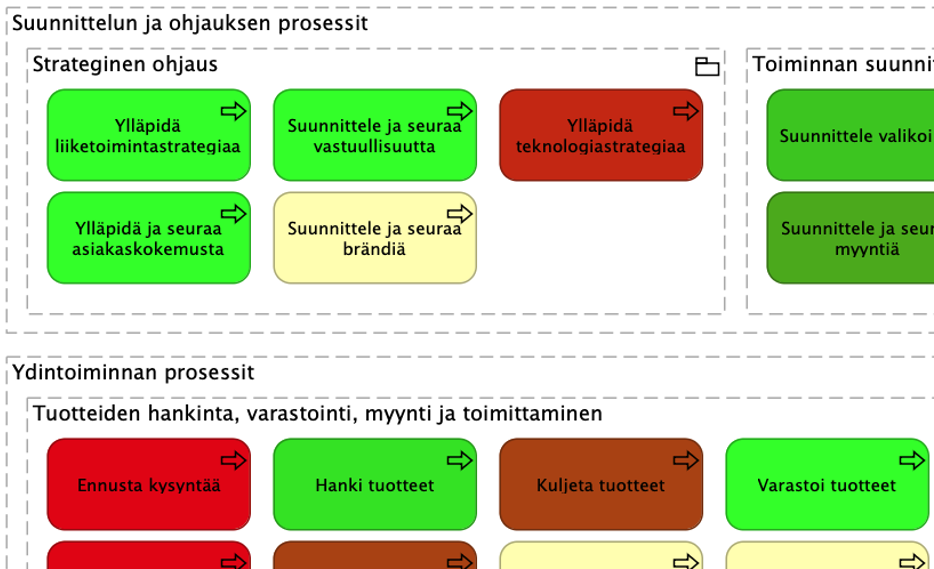
\includegraphics[keepaspectratio]{kuviot/am-esim7.png}}

}

\caption{\label{fig-am-esim7}Prosessien palvelevuuden
liikennevaloanalyysi KA-informaation avulla tuotettuna}

\end{figure}%

\bookmarksetup{startatroot}

\chapter{Mallit, mallintaminen ja Business Process Model and
Notation}\label{mallit-mallintaminen-ja-business-process-model-and-notation}

\section{Mallit ja mallintaminen}\label{mallit-ja-mallintaminen}

Käsitteet prosessimalli, prosessikaavio ja prosessin visualisointi ovat
tulleet jo aiemmin vastaan. Luvun ensimmäisessä osassa tarkastellaan
yleisesti, mikä malli on ja miksi malleja tehdään. Lopuksi hahmotellaan,
millainen on hyvä BPMN-malli. Prosessimallinnukseen perehdytään luvun
toisessa osassa.

\subsection{Mitä mallit ovat?}\label{mituxe4-mallit-ovat}

Malli on abstrakti kuvaus jostakin ilmiöstä tai asiasta, kuten vaikkapa
liiketoimintaprosessista. Mallin tarkoitus on auttaa ymmärtämään,
hallitsemaan tai ennakoimaan jotain kohdetta tai kokonaisuutta tai sen
toimintaa. Mallit ovat siis todellisuutta (mennyttä, nykyistä tai
mahdollista tulevaa) kuvaavia abstrahoituja esityksiä, jotka säilyttävät
ja välittävät kohdealuetta koskevaa tietoa. Abstrahointi tarkoittaa
sitä, että monimutkaisesta ilmiöstä tai ongelmasta pyritään poistamaan
epäoleelliset yksityiskohdat ja näin helpottamaan kuvattavan kohteen
käsittelyä.

Mallin keskeinen tarkoitus on tehdä kohteensa näkyväksi. Joissain
tapauksissa malleilla esitettävien kohteiden suora havainnointi on
hankalaa tai mahdotonta. Hankalasti havainnoitava asia on esimerkiksi
edellä sivuttu ukonilman syntyminen, kun taas rakennusarkkitehdit voivat
laatia malleja kohteista, joita ei ole vielä olemassakaan. Sääilmiöitä
koskevat mallit tavallaan vastaavat tai pyrkivät vastaamaan nykytilan
prosessikuvauksia, kun taas rakennusarkkitehdin laatima
arkkitehtuurisuunnitelma vertautuu tavoitetilan suunniteltuun
prosessikulkuun\sidenote{\footnotesize Tilastotieteilijä George Box on todennut, että
  ''\emph{All models are wrong, but some are useful}'' eli kaikki mallit
  ovat virheellisiä, mutta jotkin niistä ovat hyödyllisiä. Tämä
  kannattaa pitää mielessä, puhuttiinpa sitten Boxin alan
  tilastomatemaattisista malleista tai muista ilmiöitä abstrahoivista ja
  yleistävistä malleista, kuten prosessimalleista.}.

Mallit voidaan jakaa kahteen pääkategoriaan: kuvaileviin malleihin
(jotka kuvaavat nykyistä tilannetta) ja suunnittelumalleihin (jotka
tukevat muutoksen suunnittelua ja toteutusta)\sidenote{\footnotesize On olemassa
  lukuisia muitakin mallityyppejä, kuten ennustavat mallit
  (\emph{predictive model}), joiden avulla pyritään ennakoimaan tulevaa
  eli jonkin kohteen tai ilmiön käyttäytymistä ja analyyttiset mallit
  (\emph{analytical model}), jotka rikastavat mallin kohteen tarkastelua
  matemaattisten funktioiden, kuten differentiaaliyhtälöiden, ja
  määrällisen analyysin avulla.}. Kuvailevat mallit esittävät jotain
olemassa olevaa asiaa tai ilmiötä, kuten vaikkapa rautatieverkostoa,
asuinrakennusta, organisaation kokonaisarkkitehtuuria, tietojärjestelmää
tai prosessia. Kuvailevia malleja voidaan käyttää esimerkiksi
hallittaessa jotain monimutkaista kokonaisuutta, tunnistettaessa
tarkasteltavan kohteen nykyisessä toteutuksessa olevia puutteita tai
arvioitaessa kohteen yhteensopivuutta sen nykyisen tai tulevan
ympäristön kanssa. Suunnittelumallien avulla puolestaan voidaan
hahmotella johonkin nykyiseen asiaan aiottavaa muutosta tai jotain, mitä
ei vielä ole -- kuten vaikkapa se rakennusarkkitehdin suunnittelema
rakennus. Suunnittelumalleja tarvitaan ensinnäkin suunnitellun muutoksen
toteuttamiskelpoisuuden arviointiin ja sen jälkeen muutoksen
toteuttamisen tueksi.

Lisäksi mallit voidaan jakaa epäformaaleihin, puoliformaaleihin ja
formaaleihin malleihin. Oikeastaan formaalisuus on mallinnuksessa
käytettävän mallinnustavan tai -kielen ominaisuus, jota kielellä luotu
malli sitten noudattaa. Mallinnuskielen semantiikan\sidenote{\footnotesize Semantiikka
  eli merkitysoppi tutkii sanojen ja ajatusten sisältöjä, merkityksiä ja
  viittauksia. Semantiikka on kielitieteen ja filosofian alalaji, mutta
  käsitettä käytetään myös puhekielessä jokseenkin samanlaisessa
  tarkoituksessa. Mallinnuskielissä, kuten BPMN:ssä, kielen semanttisen
  määrittelyn tarkkuus liittyy siihen, kuinka tarkasti ja
  yksiselitteisesti kielen elementit on määritelty. Jos
  prosessimallintajalle on esimerkiksi epäselvää, pitäisikö tietyssä
  tilanteessa käyttää Manual Task- vai User Task -tyyppistä tehtävää, on
  kyse kielen semantiikkaan liittyvästä ongelmasta.} ja
syntaksin\sidenote{\footnotesize Syntaksi eli lauseoppi tarkastelee luonnollisen tai
  formaalin kielen merkkiyhdistelmiä (sanoja tai käsitteitä), niiden
  oikeaa muotoa (oikeinkirjoitus) ja oikeaa käyttöä (kielioppi ja
  lauserakenne). BPMN:n kaltaisissa visuaalisissa mallinnuskielissä
  käsitteiden oikeinkirjoitus on harvoin ongelma, koska sanoja vastaavat
  valmiit graafiset symbolit. Haasteet voivat sen sijaan liittyä mallien
  kielioppiin ja lauserakenteeseen, eli kuinka näitä symboleita tulisi
  käyttää kieliopillisesti oikean mallin muodostamiseksi. Samoin kuin
  suomenkielinen virke alkaa isolla alkukirjaimella ja päättyy
  lopettavaan välimerkkiin, BPMN-kielellä esitetty prosessimalli alkaa
  Start Event -tyyppisellä tapahtumalla ja päättyy End Event -tyyppiseen
  tai Terminate Event -tapahtumaan.} määrittelyn tarkkuus vaikuttaa
siihen, kuinka formaaleja malleja kielellä voidaan tuottaa. Mitä
yksiselitteisemmät ja tarkemmin määritellyt semantiikka ja syntaksi
ovat, sitä suurempi on mallien formaalisuus. Mallinnuskielen semantiikka
viittaa kielen elementtien merkityksien määrittelyyn ja syntaksilla
tarkoitetaan sääntöjä siitä, miten mallit ovat kielen avulla
rakennettavissa. Se, että tummakärkinen nuoli esittää prosessin kulkua
tehtävästä toiseen, on BPMN-kielen semantiikkaa. Vastaavasti se, että
tällainen nuoli ei voi liikkua uima-altaasta toiseen, on kielen
syntaksia koskeva määrittely.

Siinä missä epäformaalit mallit mahdollistavat viestinnällisen
joustavuuden ja mallien luovan tulkinnan, on formaalien mallien merkitys
täsmällinen. Siksi formaaleja malleja voidaan käsitellä ja tulkita
koneellisesti ja niiden syntaktinen oikeellisuus voidaan tarkastaa
automaattisesti. Epäformaaleja malleja voidaan laatia ja esittää
esimerkiksi luonnollisella kielellä tai vapaamuotoisina piirroksina ja
kaavioina. Formaalit mallinnuskielet puolestaan noudattavat ehdottoman
tarkkaa syntaksia ja semantiikkaa, ja ne usein perustuvat esimerkiksi
joukko-oppiin ja matemaattiseen logiikkaan.

Jos vapaamuotoisen kaavion elementtien merkityksiä ryhdytään
määrittelemään, lähestytään puoliformaalia esitystapaa: esimerkiksi
sovitaan, että soikiolla tarkoitetaan prosessin aikana suoritettavaa
tehtävää, kysymysmerkillä valintaa ja että kulku tehtävästä valintaan ja
takaisin ilmaistaan nuolella.

Puoliformaaleissa mallinnuskielissä käytetään enimmäkseen vakiintunutta
syntaksia (esimerkiksi graafisia symboleja), mutta niiden semantiikka ei
ole täysin yksiselitteinen ja aukoton, joten se voi vaihdella
esimerkiksi kontekstin mukaan. Puoliformaalit mallit ovat kohtalaisen
ristiriidattomasti tulkittavissa, vaikka ne eivät välttämättä olekaan
muodollisesti todistettavissa tai verifioitavissa. Käytännön kannalta
puoliformaaleissa kielissä oleellista onkin, että mallinnuskieleen
perehtymättömätkin pystyvät ainakin jossain määrin niitä tulkitsemaan,
mutta kieli on kuitenkin niin tarkasti määritelty, ettei tulkinta salli
summittaista arvailua. Vuokaavio, samoin kuin esimerkiksi UML:n luokka-,
sekvenssi-, aktiviteetti- ja käyttötapauskaaviot, ovat esimerkkejä
puoliformaaleista malleista.

Puoliformaalien kielten käyttötavan formaalisuuden asteesta voidaan
sopia tapauskohtaisesti ja tarpeen mukaan. Tähän liittyy sekä hyötyjä
että haasteita. Jos puoliformaalia mallinnuskieltä käytetään
epäformaalisti, mutta näin laadittua mallia toisessa yhteydessä
tulkitaankin kirjaimellisesti, on väärinymmärryksen riski olemassa.
Formaalimman mallin epäformalisointi on useimmiten helppoa, mutta
epäformaalin esityksen formalisointi mahdotonta tai vähintäänkin
hankalaa. Sen vuoksi puoliformaaleja mallinnuskieliä on järkevää pyrkiä
käyttämään mahdollisimman tarkasti ja oikein.

\subsection{Hyvä BPMN-malli}\label{hyvuxe4-bpmn-malli}

BPMN on mallinnuskielenä sikäli mielenkiintoinen tapaus, että sen
graafinen notaatio (syntaksi) näyttäytyy muodoltaan puoliformaalina --
tai sitä ainakin usein käytetään puoliformaaliin ja joskus jopa
epäformaaliin tyyliin -- kun taas BPMN:n XML-muotoinen esitystapa on
sekä syntaksiltaan että semantiikaltaan varsin formaali. BPMN:n
XML-muotoinen määritys mahdollistaa prosessimallien koneellisen
lukemisen, mikä edelleen tekee mahdolliseksi mallintaa koneellisesti ja
täysin automaattisesti suoritettavia työnkulkuja BPMN:n graafisen
notaation avulla.

BPMN-malli esittää -- tai ainakin sen tulisi esittää -- kaikki
mahdolliset tapaukset, joiden mukaisesti prosessi voi edetä. Esimerkiksi
jokin tilauskäsittelyprosessi toteutuu tietyllä tavalla, mikäli käsillä
oleva tilaus on kotimaan tilaus ja toisella tavalla, jos kyseessä on
ulkomaan tilaus.

Prosessimalli esittää molemmat tapaukset ja tietysti muutkin prosessin
vaihtoehtoiset kulut, valinnat ja erikoistilanteet. Prosessimallin
yksittäisiä suoritus-, toteutus- tai ajokertoja kutsutaan
prosessi-instansseiksi. Instanssit voivat olla erilaisia, vaikka ne
perustuvatkin samaan prosessimalliin. Prosessimalli siis määrittelee
prosessin ''ratkaisuavaruuden''.

Automaattisesti suoritettavia prosesseja mallinnettaessa tietysti myös
graafista notaatiota tulee pyrkiä käyttämään mahdollisimman
oikeellisesti eli kielen spesifikaation\sidenote{\footnotesize https://www.omg.org/spec/BPMN}
mukaisesti. Luova soveltaminen voi johtaa lopputulokseen, jossa prosessi
ei toimi oikealla tavalla -- jos toimii ollenkaan.

Joskus kuulee, että jotain asiaa pitäisi ''katsoa oksalta''. Usein onkin
järkevää pyrkiä tarkastelemaan esimerkiksi käsillä olevaa ongelmaa ensin
hieman korkeammalta ja abstrahoiden: kokonaisvaltaisesti ja
yksityiskohtiin puuttumatta. Vaikkapa jotain prosessia tarkasteltaessa
saattaa kuitenkin olla vaikea tietää, mitkä siihen liittyvät asiat ovat
ehdottoman oleellisia ja mitkä tarpeettomia yksityiskohtia.

Jo aiemmin nähdyssä pizzatilauksen prosessissa
(kuva~\ref{fig-pizzatilaus}) oletettiin, että tilattu pizza onnistutaan
aina valmistamaan. Entä sitten, jos raaka-ainevarastosta onkin ananas
päässyt loppumaan ja kuinka ravintolan silloin tulisi toimia
tilanteessa, jossa asiakas tilaa \emph{Tropicana}-pizzan?
Asiakaspalvelija ottaa tilauksen vastaan ja välittää tiedon keittiöön.
Kokki huomaa ananaksen olevan lopussa, joten tilausta ei pystytä
toteuttamaan. Kertooko kokki asiakaspalvelijalle, että ananasta
sisältäviä pizzoja ei enää tänään tehdä? Soittaako asiakaspalvelija
äskeisen tilauksen tehneelle asiakkaalle ja pahoittelee, että hänen
tilaustaan ei voida toimittaa? Onneksi prosessi oli kuitenkin
suunniteltu niin, että maksu kerätään asiakkaalta vasta pizzan
toimituksen yhteydessä. Muutoin asiakkaan maksusuoritus täytyisi
palauttaa, josta edelleen syntyisi tarpeetonta ja arvoa tuottamatonta
vaivaa. Vai tulisiko kokin sännätä tukkuun hakemaan lisää ananasta?
Tuskin kokin, koska hänellä on toiminnan kannalta kriittinen rooli
pizzojen valmistamisessa. Kuka kauppaan sitten ehtisi ja entä jos kaupat
ovat jo kiinni? Ja niin edelleen.

\begin{figure}

\centering{

\pandocbounded{\includegraphics[keepaspectratio,alt={Klassinen esimerkki pizzatilauksen prosessista.}]{index_files/mediabag/kuviot/pizzatilaus.pdf}}

}

\caption{\label{fig-pizzatilaus}Pizzatilausprosessi}

\end{figure}%

Pizzatilauksen prosessikaavio toisaalta osoittaa, että varsin
yksinkertaisestakin toimintoketjusta saadaan helposti rakennettua
kohtalaisen monimutkaisen näköinen prosessimalli. Kuitenkin jo yhden
samoin yksinkertaisen ja varmasti hyvin yleisen poikkeustilanteen, eli
jonkin täytteen loppumisen, tunnistaminen nosti esille useita
kysymyksiä, jotka varmasti olisi ollut syytä huomioida prosessimallia
laadittaessa.

Esimerkin pizzatilausprosessi on siis käytännön kannalta lähes
äärimmilleen yksinkertaistettu. Järkevä abstrahointi tässä tapauksessa
voisi esimerkiksi tarkoittaa, ettei prosessikulun näkökulmasta tarvitse
tietää, onko varastosta loppunut ananas, kinkkusuikaleet vai
tomaattikastike (emme siis mallintaisi prosessiin päätöstaulua tai
erillistä ehtoporttia jokaiselle täytevaihtoehdolle), vaan huomioisimme
yleisesti sen, että jokin raaka-aine saattaa loppua. Prosessimalleja
laadittaessa abstrahointi edellyttää mallintajalta toimialan tuntemusta
tai aktiivista vuorovaikutusta toimialan asiantuntijoiden kanssa. Se,
kuinka korkealta oksalta prosessia voidaan katsoa, jotta malli kuitenkin
sisältää kaiken relevantin tiedon, riippuu tilanteesta, tarpeesta ja
mallin käyttötarkoituksesta.

Kaikki mallit ovat siis enemmän tai vähemmän puutteellisia ja
virheellisiä, kun niitä verrataan todellisuuteen. Boxin keskeinen
kysymys olikin, kuinka virheellinen, puutteellinen tai abstrahoitu malli
voi olla, ennen kuin se muuttuu hyödyttömäksi.

Malli pyrkii siis esittämään tarkoituksenmukaisesti abstrahoidun
kuvauksen jostakin ilmiöstä, joka usein, mutta ei välttämättä aina,
esiintyy myös todellisuudessa. Näin ilmiötä kyetään hahmottamaan,
ymmärtämään ja ennakoimaan. Vastaavasti mallia voidaan verrata
ympäröivästä todellisuudesta saatavaan palautteeseen. Tämän tulisi
tarvittaessa johtaa mallin mukauttamiseen, täydentämiseen tai
korjaamiseen (kuva~\ref{fig-malli_vs_todellisuus}). Edellisessä
esimerkissä se, että prosessimalli ei huomioinut täytteen mahdollista
loppumista, voisi olla todellisuuden esiin nostama palaute, joka
johtaisi prosessimallin tarkentamiseen.

\begin{figure}

\centering{

\pandocbounded{\includegraphics[keepaspectratio]{index_files/mediabag/kuviot/malli_vs_todellisuus.pdf}}

}

\caption{\label{fig-malli_vs_todellisuus}Mallin ja todellisuuden suhde}

\end{figure}%

Edellistä ajatusta voidaan hieman mutkistaa yli sata vuotta sitten
esitellyn kielitieteeseen ja semiotiikkaan liittyvän semioottisen
kolmion (Ogden ja Richards 1923) avulla. Mallissa on kolme
pääkomponenttia: \emph{referent} (tarkoite), \emph{symbol} (symboli,
merkitsijä) ja \emph{thought} tai \emph{reference} (ajatus, referenssi).
Tarkoite on jokin todellisen maailman asia tai ilmiö, esimerkiksi
henkilö, tietojärjestelmä tai vaikkapa liiketoimintaprosessi. Symboli on
konkreettinen kieliyksikkö, kuten sana, kuva tai ääni, joka toimii
viittauksena tarkoitteeseen. Henkilöön voitaisiin tietyssä kontekstissa
viitata hänen nimellään tai vaikkapa tehtävänimikkeellä
'tilauskäsittelijä'. Tilauskäsittelyprosessiin viittaavana symbolina
voisi -- tietysti prosessin nimen lisäksi -- toimia prosessimalli.
Semioottisen kolmion kolmas komponentti on ajatus (tai referenssi), joka
on jonkinlainen mentaalinen representaatio, jonka symboli herättää
mielessämme. Symboli tai sana ei viittaa suoraan kohteeseensa, eli sitä
vastaavaan todelliseen asiaan, vaan se viittaa ensin mieleemme
ajatuksena muodostuvaan käsitteeseen, jonka avulla ymmärrämme, mihin
todellisuuden ilmiöön symboli viittaa. Jos emme tunne jotakin näistä
kolmesta komponentista, ei merkitysyhteyttä muodostu. Jos emme tunne
kuulemaamme sanaa tai ymmärrä näkemäämme graafista mallia, emme pysty
yhdistämään symbolia tarkoitteeseen. Vaikka symboli olisi meille
sinällään tuttu, mutta se ei muodosta mieleemme järkiperäistä ajatusta,
emme pysty yhdistämään sitä oikeaan kohteeseen reaalimaailmassa.
Saatamme esimerkiksi muistaa kuulleemme jonkin vierasperäisen sanan
aiemminkin, mutta jos sana ei juuri nyt soita päässämme mitään kelloja,
emme pysty yhdistämään sitä tarkoitteeseen. Yhteys symbolin (symbol) ja
tarkoitteen (referent) välillä on siis epäsuora yhteys, ja niiden väliin
tarvitaan ihmisen mielessä oleva viittaava ajatus tai käsitys
(reference).

Semiotiikan näkökulmasta edellinen korostaa, että kielen ja
todellisuuden suhde ei ole yksiselitteinen. Sama koskee tietenkin myös
mallinnuskieliä. Prosessimalli on eräänlainen symboli tai merkitsijä;
visuaalinen tai formaali esitys, joka viittaa johonkin todelliseen
toimintaan organisaatiossa. Mallin ja todellisuuden välillä on aina
käsitteellistä tulkintaa. BPMN-malli ei siis lähtökohtaisesti kuvaa
todellista prosessia, vaan lähinnä mallintajan tulkintaa tai ymmärrystä
siitä\sidenote{\footnotesize Tosin prosessimoottorilla suoritettavan täysin
  automatisoidun prosessin BPMN XML -kuvaus merkitsijänä on käytännössä
  sama kuin sen tarkoite.} (kuva~\ref{fig-semiotic_tri}).

\begin{figure}

\centering{

\pandocbounded{\includegraphics[keepaspectratio]{index_files/mediabag/kuviot/semiotic_tri.pdf}}

}

\caption{\label{fig-semiotic_tri}Semioottinen kolmio}

\end{figure}%

Palataan vielä hetkeksi tapaukseen, jossa pizzerian keittiössä ananas
oli päässyt loppumaan. IT-orientoitunut ihminen saattaisi ehdottaa
ratkaisuksi vaikkapa yksinkertaista inventaariohallintajärjestelmää.
Järjestelmä voisi välittää tilauksia vastaanottavalle
asiakaspalvelijalle tiedon, kun ananas alkaa käydä vähiin. Tämä olisi
varsin helppoa, mikäli järjestelmän tiedot päivittyisivät sisäänostojen
ja myyntien perusteella. Edelleen järjestelmä voisi ananaksen loppuessa
automaattisesti muuttaa ananasta tarvitsevien pizzojen tilaksi
''loppuunmyyty''.

Malleihin, mallien laatimiseen ja niiden käyttöön liittyy myös riskejä,
koska niiden jo määritelmällisestikin oletetaan kuvaavan todellisuutta,
mutta toisaalta ne ovat lähes aina myös jollain tavalla puutteellisia.
Ajatellaan, että pizzeria päättäisi hankkia joltain ohjelmistotalolta
verkkotilausjärjestelmän. Osana järjestelmän
vaatimusmäärittelydokumentaatiota pizzeria tarjoaisi edellä nähdyn
prosessimallin (kuva~\ref{fig-pizzatilaus}), ja järjestelmä
rakennettaisiin sen mukaisesti. Järjestelmä ja erityisesti pizzerian
toiminta alkaisivat yskähdellä heti, kun saapuu tilaus, jota jonkin
raaka-aineen loppumisen vuoksi ei kyettäisi toimittamaan. Järjestelmä
sinällään toimisi vaatimusten mukaisesti, mutta koska toiminnalliset
vaatimukset olivat puutteellisen ja epätarkan prosessimallin vuoksi
esitetty yhtä lailla puutteellisesti ja epätarkasti, ei järjestelmä
vastaisi liiketoiminnan tarpeita. Tämä korostaa liiketoiminnan
ymmärtämisen merkitystä prosessimalleja laadittaessa. Sen puuttuessa
taitavakaan mallintaja ei pysty tuottamaan hyvää prosessimallia.
Yhteenvetona: hyvä prosessimalli

\begin{itemize}
\tightlist
\item
  vastaa käyttötarkoitustaan,
\item
  perustuu tietoon, joka on kerätty useista eri tietolähteistä,
\item
  edustaa liiketoimintatuntemusta,
\item
  on katselmoitu ja varmennettu laajan asiantuntijajoukon toimesta,
\item
  ei sisällä syntaktisia, semanttisia tai loogisia virheitä,
\item
  on ymmärrettävä, visuaalisesti selkeä ja tekee prosessitiedosta
  läpinäkyvää.
\end{itemize}

Mendling ym. (2010) ovat esittäneet seitsemän konkreettista ohjetta
prosessimallintajille. Tutkimusta tehdessään he huomasivat, että nämä
ohjeet saattavat olla joissain tapauksissa keskenään ristiriitaisia.
Esimerkiksi yksi ohjeista on, että mallin tulisi sisältää mahdollisimman
vähän elementtejä, kun taas toinen ohje kuuluu, että reititysten määrä
tulisi pyrkiä minimoimaan. Siinä missä pienempi määrä elementtejä tekee
mallista helpommin ymmärrettävän, reitityspolkujen karsimisesta usein
seuraa tarve lisätä elementtien määrää. Tämän vuoksi Mendling ym. (2010)
priorisoivat ohjeet perustuen keskusteluihinsa prosessimallinnuksen
asiantuntijoiden ja ammattilaisten kanssa. Mikäli ohjeet asettavat
mallille ristiriitaisia vaatimuksia, tulee niitä soveltaa
prioriteettijärjestyksessä. Mendlingin ym. (2010)\sidenote{\footnotesize Näihin
  ohjeisiin kannattaa palata uudelleen, kun on perehtynyt BPMN-kieltä
  käsittelevään osuuteen.} ohjeet ovat:

\begin{enumerate}
\def\labelenumi{\arabic{enumi}.}
\tightlist
\item
  Käytä mallissa mahdollisimman vähän elementtejä. Mallin suuri koko
  heikentää sen ymmärrettävyyttä ja lisää virheiden mahdollisuutta.
\item
  Minimoi reitityspolkujen määrä per elementti. Mitä suurempi elementin
  aste prosessimallissa on (eli yhteenlaskettu sisään tulevien ja ulos
  lähtevien virtojen (\emph{sequence flow}) määrä), sitä vaikeampi
  mallia on ymmärtää. Mendlingin ym. (2010) artikkelissa viitattujen
  tutkimusten mukaan elementtien määrällä ja asteilla on vahva
  korrelaatio mallinnusvirheiden määrän kanssa.
\item
  Käytä yhtä aloitustapahtumaa ja yhtä lopetustapahtumaa. Myös aloitus-
  ja lopetustapahtumien määrän kasvu on yhteydessä virheiden
  todennäköisyyden kasvuun ja hankaloittaa mallin ymmärtämistä. Yhtä
  aloitus- ja lopetustapahtumaa käyttävien mallien oikeellisuuden
  tarkastaminen on helpompaa. Lisäksi useimmat
  työnkulkuautomaatiojärjestelmät edellyttävät yhtä aloitus- ja
  lopetustapahtumaa\sidenote{\footnotesize Tämä tosin ei pidä paikkaansa esimerkiksi
    Camundassa.}.
\item
  Mallinna mahdollisimman rakenteisesti. Tällä tarkoitetaan, että
  jokaiselle prosessivirran jakavalle portille tulee vastinparina
  mallista löytyä samaa tyyppiä oleva yhdistävä portti. Tämä vertautuu
  esimerkiksi ohjelmakoodissa tai matemaattisissa lausekkeissa
  käytettyihin sulkumerkkeihin: jokaisella avaavalla sulkumerkillä tulee
  olla sulkeva pari. Tutkimusten mukaan rakenteettomissa malleissa
  virheiden todennäköisyys on suurempi, ja ihmiset myös ymmärtävät niitä
  huonommin.
\item
  Vältä OR-reitityselementtejä. Mendling ym. (2010) neuvovat välttämään
  OR- eli \emph{Inclusive Gateway} -päätösportteja, koska tutkimusten
  mukaan niihin liittyy helposti semanttista epäselvyyttä ja
  toteutusongelmia. AND- (\emph{Parallel Gateway}) ja XOR-portit
  (\emph{Exclusive Gateway}) on todettu vähemmän virhealttiiksi.
\item
  Käytä aktiviteettien nimissä verbi-objekti -muotoa. Tutkimuksissa,
  joissa on tarkasteltu todellisissa prosessimalleissa käytettyjä
  nimeämiskäytänteitä, on kahdeksi vallitsevaksi tyyliksi tunnistettu
  verbi-objektia (esimerkiksi ''Käsittele reklamaatio'') sekä
  aktiviteetin teon nimeä (esimerkiksi ''Reklamaation käsittely'')
  käyttävät muodot. Kolmas yleisesti käytetty tyyli on nimetä
  aktiviteetit epämääräisemmin toiminnan kontekstilla (esimerkiksi
  ''Reklamaatio''). Mendling ym. (2010) ehdottavat verbi-objekti -muotoa
  parhaaksi käytänteeksi.
\item
  Jaa malli osiin, mikäli siinä on yli 50 elementtiä. Mallin koon ja
  virheiden välillä on todettu olevan voimakas positiivinen korrelaatio.
  Mendlingin ym. (2007) toisen tutkimuksen mukaan malleissa, joissa on
  yli 50 elementtiä, on virheiden todennäköisyys taipuvainen kasvamaan
  yli 50 prosentin. Näin ollen he suosittelevatkin, että suuret mallit
  tulisi jakaa pienemmiksi osamalleiksi. Huomautettakoon kuitenkin, että
  osiin jaettujen mallien ylläpito sekä niiden koherenssin ja
  konsistenssin toteuttaminen voi olla yksittäistä, suurtakin, mallia
  hankalampaa. Useimmat prosessimallinnusvälineet osaavat kuitenkin
  haluttaessa piilottaa aliprosessien tarkemman työnkulun, jolloin
  monimutkainen malli on mahdollista näin jakaa osiin ja myös mallintaa
  osissa, vaikka mallia ei tosiasiassa pilkottaisikaan.
\end{enumerate}

Seuraavassa taulukossa (Taulukko~\ref{tbl-7pmg}) on esitetty edellisten
ohjeiden järjestys kuten prosessiasiantuntijat ne näkivät. Ohjeita
tulisi siis noudattaa niiden prioriteetin mukaisessa järjestyksessä,
mikäli ne jossain tapauksessa asettuvat keskenään ristiriitaan.

\begin{longtable}[]{@{}clr@{}}
\caption{Prosessimallinnuksen seitsemän ohjetta
prioriteettijärjestyksessä}\label{tbl-7pmg}\tabularnewline
\toprule\noalign{}
Prioriteetti & Ohje & Kumulatiivinen sija \\
\midrule\noalign{}
\endfirsthead
\toprule\noalign{}
Prioriteetti & Ohje & Kumulatiivinen sija \\
\midrule\noalign{}
\endhead
\bottomrule\noalign{}
\endlastfoot
1 & Mallinna mahdollisimman rakenteisesti. & 58,5 \\
2 & Jaa malli osiin, mikäli siinä on yli 50 elementtiä. & 73,5 \\
3 & Käytä mallissa mahdollisimman vähän elementtejä. & 80,5 \\
4 & Käytä aktiviteettien nimissä verbi-objekti-muotoa. & 84,0 \\
5 & Minimoi reitityspolkujen määrä per elementti. & 86,5 \\
6 & Käytä yhtä aloitustapahtumaa ja yhtä lopetustapahtumaa. & 101,0 \\
7 & Vältä OR-reitityselementtejä. & 104,0 \\
\end{longtable}

\section{Business Process Model and
Notation}\label{business-process-model-and-notation}

\emph{Business Process Model and Notation}\sidenote{\footnotesize https://www.omg.org/spec/BPMN/2.0/}
(BPMN) on \emph{Object Management Groupin}\sidenote{\footnotesize https://www.omg.org/}
(OMG) ylläpitämä kansainvälinen standardi liiketoimintaprosessien
graafiseen mallintamiseen. Se on tarkoitettu yhteiseksi välineeksi
liiketoiminta-analyytikoille, ohjelmistokehittäjille ja muille
prosessien parissa työskenteleville sidosryhmille. BPMN:n visuaalinen
esitystapa pyrkii mahdollistamaan prosessien kuvaamisen johdonmukaisella
ja helposti ymmärrettävällä tavalla ja siten parantamaan kommunikaatiota
liiketoiminnan ja IT:n välillä\sidenote{\footnotesize Tosin BPMN 2.0 -standardin
  spesifikaatio itsessään on yli 500 sivua.
  https://www.omg.org/spec/BPMN/2.0/PDF}. Graafiset BPMN-mallit ovat
esitettävissä myös XML:ään (Extensible Markup Language) perustuvalla
koneluettavalla kielellä (BPMN XML), jota käyttäen prosessimallit ovat
automatisoitavissa eli suoritettavissa prosessimoottoreiksi
kutsuttavilla ohjelmistoilla.

BPMN:n tarina käynnistyi 2000-luvun alkuvuosina, kun \emph{Business
Process Management Initiative} (BPMI) -niminen organisaatio alkoi
kehittää standardia liiketoimintaprosessien kuvaamiseen. Alusta lähtien
tavoitteena oli luoda graafinen esitystapa, joka olisi yhteensopiva
prosessien suorittamisen ja automatisoinnin kanssa. BPMN:n ensimmäinen
versio julkaistiin 2004. Seuraavana vuonna BPMI yhdistyi OMG:n kanssa,
joka ryhtyi kehittämään BPMN:stä virallista, laajemmin hyväksyttyä
standardia.

Vuosien 2006--2009 aikana julkaistut versiot keskittyivät pääasiassa
prosessien kuvaamiseen graafisesti, ja koneellisesti suoritettavien
prosessimallien tuki oli vielä melko rajallinen. Vuonna 2011 julkaistu
BPMN 2.0 oli merkittävä kehitysharppaus. Samassa yhteydessä julkaistun
uuden metamallin tarkkuus mahdollisti prosessimallien koneellisen
tulkinnan ja automaattisen suorittamisen. Mallinnuskielen elementtien
valikoima kasvoi ja virallinen XML-pohjainen tiedostomuoto
julkistettiin. BPMN 2.0 on edelleen kielen nykyinen versio, ja siihen on
toistaiseksi julkaistu ainoastaan joitain pieniä korjauksia ja
selvennyksiä. Versionumeroinnin desimaaleja tarkemmin tarkasteltaessa
BPMN:n viimeisin versio tätä kirjoitettaessa on 2.0.2 ja se julkaistiin
tammikuussa 2014. Se tunnetaan myös ISO/IEC -standardina numerolla 19510
ja nimellä Information technology -- Object Management Group Business
Process Model and Notation\sidenote{\footnotesize Edition 1 vuodelta 2013
  https://www.iso.org/standard/62652.html}.

BPMN on paitsi virallinen standardi myös \emph{de facto} -standardi
liiketoimintaprosessien mallinnuksessa, organisaatioiden sisäisessä
kehitystyössä, prosessien optimoinnissa sekä prosessien
automatisoinnissa ja monitoroinnissa. Sitä tukevat lukuisat työvälineet,
joista yksi on kirjan prosessiesimerkeissäkin käytetty \emph{Camunda
Modeler}\sidenote{\footnotesize https://camunda.com/platform/modeler/}.

Seuraavissa alaluvuissa käydään läpi BPMN 2.0:n ominaisuuksia prosessien
graafisessa mallintamisessa. Vaikka niissä käsitellään BPMN-kieli
kokonaisuudessaan, todettakoon, että varsin pieni osajoukko kielen
elementtejä riittää varsin pitkälle yksinkertaisten ja ainoastaan
ihmisten luettaviksi tarkoitettujen prosessien suunnittelussa,
dokumentoinnissa ja viestinnässä. BPMN sisältää kuitenkin useita
hienostuneempia elementtejä ja ominaisuuksia monimutkaisempien ja
yksityiskohtaisempien prosessikulkujen esittämiseksi sekä niiden
automatisoimiseksi.

Palataan vielä kerran hetkeksi pizzatilausesimerkin
(kuva~\ref{fig-pizzatilaus.svg}) pariin.

\begin{figure}

\centering{

\pandocbounded{\includegraphics[keepaspectratio,alt={Klassinen esimerkki pizzatilauksen prosessista.}]{index_files/mediabag/kuviot/pizzatilaus.pdf}}

}

\caption{\label{fig-pizzatilaus.svg}Pizzatilausprosessi}

\end{figure}%

Esimerkissä on kaksi uima-allasta eli kaksi erillistä toimijaa: asiakas
ja pizzeria. Pizzeria-altaan sisällä on kolme uimarataa eli roolia:
asiakaspalvelija, kokki ja lähetti. Nämä on esitetty uimaratoina saman
altaan sisällä, koska ne edustavat samaa toimijaa eli pizzeriaa. Jos
pizzan toimittamiseen käytettäisiin ulkoista lähettipalvelua, tulisi se
esittää prosessissa omana uima-altaanaan.

Laatikot esittävät prosessiin liittyvää tekemistä: \emph{Tilaa pizza},
\emph{Valmista pizza}, \emph{Toimita pizza} ja niin edelleen. Kuten
edellä todettiin, tehtävien nimeämisessä on suositeltavaa käyttää
verbi-objekti-muotoa.

Tehtäviä yhdistävät nuolet esittävät prosessin kulkua eli sitä, missä
järjestyksessä prosessin tehtävät etenevät. Katkoviivalla esitetyt
nuolet ovat puolestaan viestivirtoja ja esittävät organisaatioiden
välillä liikkuvaa tietoa. Prosessin suorittaminen voi siirtyä
uima-altaasta toiseen, eli organisaatiolta toiselle, ainoastaan
viestivirtojen kautta. Kun prosessi tapahtuu saman organisaation
sisällä, eli saman altaan uimaradoilla, liikkuu tieto prosessikulun ja
kontekstin mukana. Tällöin käytetään ainoastaan tavallisia prosessin
kulkua esittäviä nuolia ja tarvittaessa data-assosiaatiosuhdetta. Saman
uima-altaan sisällä ei siis voida käyttää viestivirtoja esittäviä
katkonuolia, eikä uima-altaasta toiseen voida siirtyä muuten kuin
viestivirtoja käyttäen.

Ympyrän muotoisilla symboleilla esitetään prosessin aikana toteutuvia
tapahtumia. Tapahtumat eroavat tehtävistä siinä, että ne eivät ole
tekemistä, jonka jokin prosessiin osallistuva toimija suorittaisi, vaan
ne pikemminkin -- nimensä mukaisesti -- ''tapahtuvat'', ja signaalien
tai herätteiden tapaan saavat aikaan muutoksen prosessin tilassa.
Prosessin aloitus ja lopetus ovat tapahtumia. Aloituksen ja lopetuksen
lisäksi tapahtumia voi esiintyä myös prosessikulun aikana.
Pizzatilausesimerkissä on viisarikellon näköinen tapahtuma, joka on
nimetty \emph{60 minuuttia}. Tämä tapahtuma aktivoituu silloin, kun 60
minuuttia on kulunut. Tällöin prosessikulku etenee tapahtumaan liittyvää
haaraa ja asiakas suorittaa tehtävän \emph{Tiedustele pizzaa}. On myös
mahdollista, että pizza toimitetaan asiakkaalle alle tunnissa, jolloin
tapahtuma \emph{60 minuuttia} ei ehdi toteutua. Tapahtumat ovatkin
ehdollisia, ja niiden avulla prosessi voidaan saada reagoimaan myös
poikkeustilanteisiin.

Vinoneliösymboleilla esitetään portteja, jotka määrittävät prosessin
kulun haarautumista, yhdistymistä ja synkronointia. Näissä kohdissa
tehdään päätös siitä, kuinka prosessin kulku etenee. Ne voivat
esimerkiksi ohjata tilanteen mukaan prosessin vaihtoehtoisiin suuntiin
tai ne voivat jakaa prosessin useampaan rinnakkain suoritettavaan
haaraan.

\subsection{Virrat ja yhteydet}\label{virrat-ja-yhteydet}

Aloitetaan BPMN:n tarkempi läpikäynti käsittelemällä erilaiset nuolet ja
viivat, joita käytetään graafisissa prosessimalleissa. Yhteys- tai
liitosviivalla (\emph{Association}) (kuva~\ref{fig-association}) ei
oikeastaan ole muuta käyttöä kuin se, että sillä voidaan liittää
huomauksia (\emph{Text Annotation}) prosessimalliin tai johonkin sen
osaan. Huomautukset sisältävät ainoastaan ihmisille tarkoitettua
informaatiota, kuten prosessia koskevaa dokumentaatiota, eivätkä ne tai
Association-suhde vaikuta prosessin kulkuun.

\begin{figure}

\centering{

\pandocbounded{\includegraphics[keepaspectratio]{index_files/mediabag/kuviot/association.pdf}}

}

\caption{\label{fig-association}Prosessimalliin Association-yhteydellä
liitettyjä huomautuksia}

\end{figure}%

Vaikka prosessimalliin lisätyt huomautukset ja kommentit eivät mallia
varsinaisesti kaunista, on niiden runsas käyttäminen kuitenkin
suositeltavaa. Hankalasti seurattavia tai monimutkaisia prosessikulkuja
voidaan dokumentoida ohjelmakoodin kommenttien tavoin.
Prosessikehittäjät ja mallintajat voivat käyttää niitä jättääkseen
toisilleen -- tai miksei itselleenkin -- kysymyksiä, huomautuksia tai
selvennyksiä: ''\emph{Toimiiko tämä näin?}'', \emph{''Tämä kohta täytyy
vielä varmistaa myymäläpäälliköiltä!}'', ''\emph{Päivämäärämuuttujan
arvo tulee Oraclesta amerikkalaisessa muodossa. Se käännetään tällä
skriptillä suomalaiseen muotoon ja tallennetaan muuttujaan pvm.}''

Dokumentaatio myös helpottaa prosessimallin ymmärtämistä silloin, kun
prosessin katselija ei ole BPMN-kielen asiantuntija. Annotaatioiden
avulla voidaan myös tehdä näkyväksi toimintoja, jotka eivät välttämättä
prosessin graafisessa esityksessä tule esille. Tällaisia tapauksia ovat
esimerkiksi myöhemmin käsiteltävät \emph{Script}- ja \emph{Business
Rule} -tehtävät.

Toinen prosessimalleissa käytettävä assosiaatiosuhte on \emph{Data
Association}, jonka avulla voidaan esittää prosessin ja tietovaraston
(\emph{Data Store}) välillä toteutuvia tietovirtoja. Yhteyttä, jossa
prosessista liikkuu tietoa tietovarastoon, kutsutaan nimellä \emph{Data
Output Association}. Kun ilmaistaan tiedon siirtymistä tietovarastosta
prosessille, yhteyttä kutsutaan nimellä \emph{Data Input Association}
(kuva~\ref{fig-data_association}). Data Storea ja Data Associationia
käsitellään hieman tarkemmin myöhemmin tässä luvussa.

\begin{figure}

\centering{

\pandocbounded{\includegraphics[keepaspectratio]{index_files/mediabag/kuviot/data_association.pdf}}

}

\caption{\label{fig-data_association}Data Store ja siihen liittyvät Data
Input Association- ja Data Output Association -yhteydet}

\end{figure}%

\emph{Sequence Flow} eli järjestysvirta ilmaisee, kuinka prosessi etenee
ja missä järjestyksessä sen elementit luetaan. Virran avulla yhdistetään
samaan prosessiin kuuluvat tapahtumat, tehtävät ja portit. Huomaa, että
prosessin jokaisen elementin täytyy liittyä virralla vähintään yhteen
toiseen elementtiin. Mikäli prosessin tehtävään ei johda järjestysvirta,
ei tehtävä voi tulla suoritetuksi. Vastaavasti prosessi jumiutuu
tehtävään, josta ei lähde järjestysvirtaa ulos. BPMN ei salli virran
ylittävän uima-altaan reunoja. Prosessin kulku ei siis voi virrata
organisaatiosta toiseen. Järjestysvirta esitetään tavallisesti
yhtenäisellä viivalla, jossa on nuolenkärki.

BPMN-kielessä virrasta eli Sequence Flow:sta on kaksi erikoisversiota:
\emph{Conditional Flow} sekä \emph{Default Flow}. Conditional Flow on
ehdollinen järjestysvirta, jota pitkin edetään vain, jos jokin
määritelty ehto täyttyy. Sitä voidaan käyttää toteuttamaan
\emph{Exclusive}- ja \emph{Inclusive} -päätösportteja vastaavaa
toiminnallisuutta. Päätösportteja käsitellään myöhemmin tässä luvussa.
Conditional Flow'n käyttö on kuitenkin melko harvinaista, koska sama
logiikka voidaan esittää myös päätösportteja käyttäen. Conditional Flow
ilmaistaan virtanuolen alussa olevalla valkoisella viistoneliöllä.

Default Flow'n avulla voidaan määritellä oletusvirta, jota seurataan,
ellei mikään ehto täyty tai jos useampi ehto täyttyy samanaikaisesti.
Default Flow ilmaistaan virtanuolta leikkaavalla vinolla poikkiviivalla.
Oletusvirran määrittely on suositeltavaa aina päätösportteja
käytettäessä. Sen avulla voidaan estää tilanne, jossa prosessi jäisi
jumiin, mikäli mikään määritellyistä ehdoista ei täyty. Toki sama
varmistus voidaan toteuttaa huolellisella if-else-rakenteen
suunnittelulla, mutta oletusvirran käyttö on helppo tapa pelata varman
päälle. (kuva~\ref{fig-sec_def_cond})

\begin{figure}

\centering{

\pandocbounded{\includegraphics[keepaspectratio]{index_files/mediabag/kuviot/seq_def_cond.pdf}}

}

\caption{\label{fig-sec_def_cond}Sequence Flow, Default Flow ja
Conditional Flow}

\end{figure}%

\emph{Message Flow} eli viestivirta kuvaa viestintää prosessien ja
organisaatioiden välillä. Viestivirtaa ei voi käyttää saman prosessin
sisällä edes silloin, kun prosessin altaassa on useampia uimaratoja, eli
samaan organisaatioon kuuluvia useampia toimijoita. Prosessin kulun
siirtyessä saman altaan ratojen välillä, vaikka siirtymän yhteydessä
siirtyisikin viestejä tai tietoa, käytetään Sequence Flow -virtaa.
Message Flow'ta käytetään silloin, kun prosessi siirtyy altaasta toiseen
(kuva~\ref{fig-message_flow}). Tällöin suorittamisen vastuu siirretään
organisaatiolta tai prosessilta toiselle.

\begin{figure}

\centering{

\pandocbounded{\includegraphics[keepaspectratio]{index_files/mediabag/kuviot/message_flow.pdf}}

}

\caption{\label{fig-message_flow}Message Flow siirtää tietoa altaiden
välillä}

\end{figure}%

\subsection{Tehtävät}\label{tehtuxe4vuxe4t}

\emph{Task} eli tehtävä esittää erilaisia prosessin aikana suoritettavia
töitä tai tehtäviä. Nämä voivat esimerkiksi olla ihmisen suorittamia
manuaalisia tai tietokoneen suorittamia automaattisia tehtäviä.
Tehtävien avulla esitetään prosessin perusrakenne.

\begin{figure}

\centering{

\pandocbounded{\includegraphics[keepaspectratio]{index_files/mediabag/kuviot/perunankuorinta.pdf}}

}

\caption{\label{fig-perunankuorinta}Yksinkertainen prosessimalli, jossa
on viisi tehtävää}

\end{figure}%

Tehtävät esitetään graafisesti tavallisesti suorakaiteen muotoisina
nelikulmioina, joiden reunat on pyöristetty. Suorakaide, jossa ei ole
mitään graafista tarkenninta (kuva~\ref{fig-perunankuorinta}), toimii
yleiskäyttöisenä tehtävien kuvauselementtinä, eikä siihen liity
suorittamista koskevia erityisiä lisätietoja. Laadittaessa
prosessimalleja vaikkapa keskustelun tueksi, voidaan tällä elementillä
esittää kaikki prosessiin kuuluvat tehtävät ja ilmaista tarvittavat
erityispiirteet tehtävän nimessä. Esimerkiksi seuraavan prosessimallin
(kuva~\ref{fig-gen_activity}) tehtävien nimistä on pääteltävissä, että
prosessiin liittyy ohjelmistorajapinnan yli suoritettavia tietokoneen
tekemiä tehtäviä sekä ihmisen suorittama tehtävä.

\begin{figure}

\centering{

\pandocbounded{\includegraphics[keepaspectratio]{index_files/mediabag/kuviot/gen_activity.pdf}}

}

\caption{\label{fig-gen_activity}Erityyppisiä tehtäviä yleisellä
tehtäväelementillä esitettyinä}

\end{figure}%

\subsubsection{Manual Task}\label{manual-task}

Ihmisen suoritettavaksi tarkoitettuja tehtävätyyppejä on kaksi.
\emph{Manual Task} on täysin manuaalinen tehtävä, esimerkiksi
paperidokumentin arkistointi tai verkkokaupassa tehtyyn tilaukseen
kuuluvien tuotteiden pakkaaminen lähetettäväksi. Manual Task merkitään
esimerkiksi kättelyasentoon ojennetun käden kuvalla
(kuva~\ref{fig-manual_task}).

\begin{figure}

\centering{

\pandocbounded{\includegraphics[keepaspectratio]{index_files/mediabag/kuviot/manual_task.pdf}}

}

\caption{\label{fig-manual_task}Manual Task ilmaisee täysin manuaalista
ihmisen suorittamaa tehtävää}

\end{figure}%

\subsubsection{User Task}\label{user-task}

Myös \emph{User Task} (kuva~\ref{fig-user_task}) ilmaisee ihmisen
suorittamaa tehtävää. Se on kuitenkin tehtävä, joka suoritetaan IT:n --
tyypillisesti jonkin ohjelmiston tai järjestelmän -- avulla. Erottelu
manuaalisten ja IT-avusteisten tehtävien välillä johtuu siitä, että
BPMN-kieltä voidaan käyttää automatisoitavien prosessien mallintamiseen,
jolloin näillä kahdella ihmisen suorittamalla tehtävällä voi olla
hyvinkin erilainen merkitys.

\begin{figure}

\centering{

\pandocbounded{\includegraphics[keepaspectratio]{index_files/mediabag/kuviot/user_task.pdf}}

}

\caption{\label{fig-user_task}User Task ilmaisee ihmisen tietokoneella
suorittamaa tehtävää, kuten tietojen syöttöä}

\end{figure}%

User Taskissa luetaan, käytetään tai tuotetaan tietoa ohjelmistoa
käyttäen, esimerkiksi täyttämällä sähköinen lomake, kun taas Manual Task
-tehtävät liittyvät tyypillisesti vuorovaikutukseen ``fyysisen
maailman'' kanssa.

\subsubsection{Script Task}\label{script-task}

\emph{Script Task} -tehtävätyypillä esitetään tehtäviä, jotka
suoritetaan prosessin aikana automaattisesti koodiskriptin avulla ilman
ihmisen osallistumista. Käytännössä siis prosessikulun saapuessa Script
Task -tehtävään, käynnistetään ennalta määritelty ohjelmakoodi, joka
tavallisesti käsittelee prosessimuuttujiin tallennettuja arvoja.

Seuraavassa esimerkissä (kuva~\ref{fig-tilauksen_hinnoittelu}) on Script
Task -tehtäviä käyttävä prosessikulku. Asiakkaalta laskutetaan 9,90 €
toimitusmaksu, ellei tilattujen tuotteiden hinta ole vähintään 100,00 €.
Esimerkissä Camunda-ympäristössä suoritettavalle prosessille tilatun
tuotteen yksikköhinnaksi annetaan 12,50 € ja niitä on tilattu kaksi
kappaletta.

\begin{figure}

\centering{

\pandocbounded{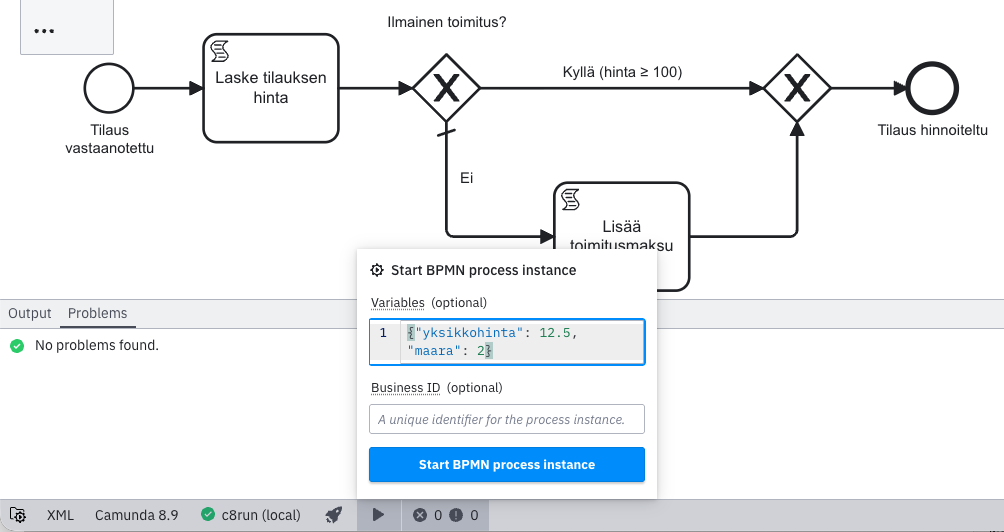
\includegraphics[keepaspectratio]{kuviot/tilauksen_hinnoittelu.png}}

}

\caption{\label{fig-tilauksen_hinnoittelu}Tilauksen kokonaishinnan
muodostaminen}

\end{figure}%

\emph{Laske tilauksen hinta} -tehtävässä lasketaan tilauksen
kokonaishinta kertomalla tilatun tuotteen \texttt{yksikkohinta}
tilaukseen kuuluvien tuotteiden määrällä \texttt{maara}. Laskutoimitus
määritellään Camundassa FEEL-skriptinä (\emph{Friendly Enough Expression
Language}), kuten (kuva~\ref{fig-kokonaishinta}).

\begin{figure}

\centering{

\pandocbounded{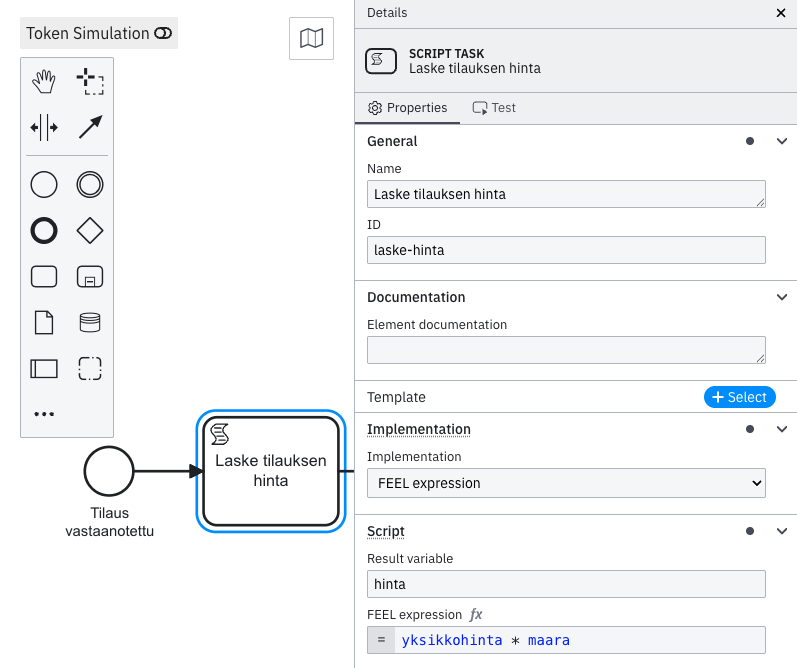
\includegraphics[keepaspectratio]{kuviot/yksikkohinta_x_maara.png}}

}

\caption{\label{fig-kokonaishinta}Laske tilauksen hinta}

\end{figure}%

BPMN-kielen graafisen esityksen taustalle prosessimallinnusvälineet
tuottavat BPMN XML -muotoista koodia. Edellinen yksinkertainen
Zeebe-skripti näyttää tältä.

\begin{Shaded}
\begin{Highlighting}[]
\NormalTok{\textless{}}\KeywordTok{zeebe:script} \OtherTok{expression=}\StringTok{"=yksikkohinta * maara"} \OtherTok{resultVariable=}\StringTok{"hinta"}\NormalTok{ /\textgreater{}}
\end{Highlighting}
\end{Shaded}

Kokonaishinta tallennetaan tulosmuuttujaan \texttt{resultVariable}
nimellä \texttt{hinta}. \emph{Laske tilauksen hinta} -tehtävää
seuraavassa portissa muuttujan arvo tarkastetaan. Koska tilauksen hinta
jää alle sadan euron (2 * 12,50 = 25,00), tilaukseen lisätään
toimitusmaksu (kuva~\ref{fig-lisataan_toimitusmaksu}).

\begin{figure}

\centering{

\pandocbounded{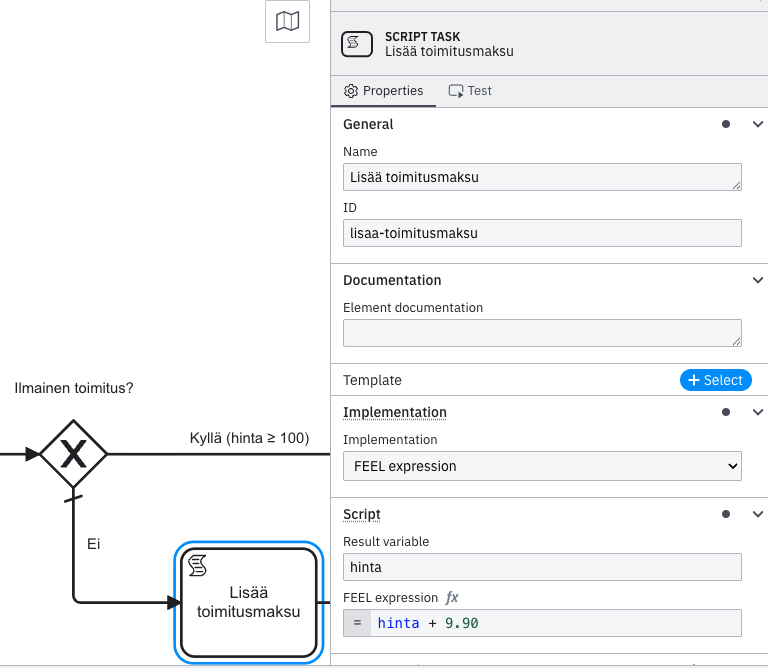
\includegraphics[keepaspectratio]{kuviot/toimitusmaksu.png}}

}

\caption{\label{fig-lisataan_toimitusmaksu}Lisätään toimitusmaksu}

\end{figure}%

Kun prosessi suoritetaan Camundan ajoympäristössä edellisillä muuttujien
arvoilla, se tuottaa seuraavan lopputuloksen
(kuva~\ref{fig-tilaus_runtime}). Koska tilaukseen lisättiin
toimitusmaksu, tuli tilauksen hinnaksi 34,90 €.

\begin{figure}

\centering{

\pandocbounded{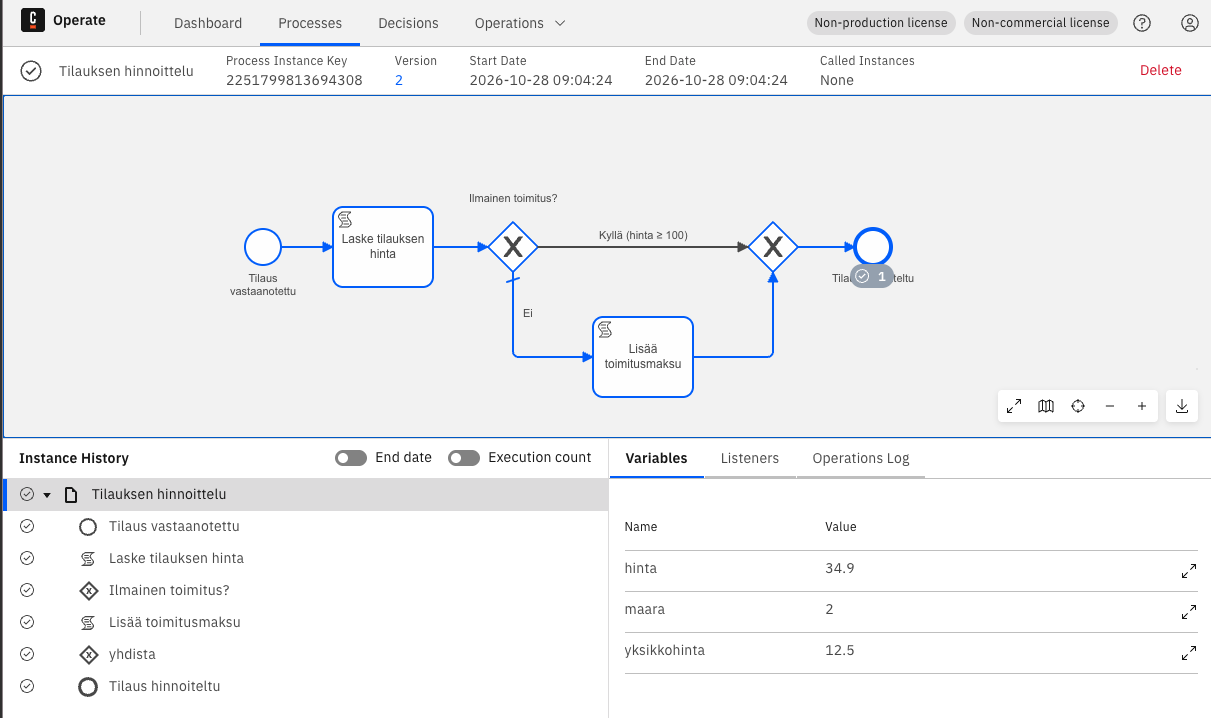
\includegraphics[keepaspectratio]{kuviot/tilaus_runtime.png}}

}

\caption{\label{fig-tilaus_runtime}Tilauksen hinnoittelu -prosessi
suoritettuna ajoympäristössä}

\end{figure}%

Seuraavassa tilauksen käsittelyn prosessimallissa käytetään kaikkia
kolmea tähän mennessä esiteltyä tehtävätyyppiä
(kuva~\ref{fig-tilauksen-kasittely-valiyhtveto}).

\begin{figure}

\centering{

\pandocbounded{\includegraphics[keepaspectratio]{index_files/mediabag/kuviot/tilauksen-kasittely-valiyhtveto.pdf}}

}

\caption{\label{fig-tilauksen-kasittely-valiyhtveto}Tilauksen käsittely}

\end{figure}%

Ensimmäinen tehtävä, Laske tilauksen hinta, on Script Task, jossa
tilauksen kokonaishinta muodostetaan suorittamalla skripti, kuten
edellä. Seuraava tehtävä on User Task, jossa myymäläpäällikkö tekee
päätöksen siitä, hyväksytäänkö saapunut tilaus vai täytyykö se jostain
syystä hylätä. Esimerkissä tilausten hyväksynnän voidaan ajatella
tapahtuvan tilaustenhallintajärjestelmässä, jota myymäläpäällikkö
käyttää. Mikäli tilaus hyväksytään, varastotyöntekijä poimii tilatut
tuotteet varastosta ja pakkaa ne lähetettäväksi. Tuotteiden pakkaaminen
on tyypiltään Manual Task.

\subsubsection{Service Task}\label{service-task}

\emph{Service Task} (kuva~\ref{fig-service_task}) on tehtävätyyppi, jota
käytetään, kun prosessissa halutaan suorittaa jokin tehtävä ulkoisen
palvelun avulla. Script Task -tehtävään verrattuna ero on siinä, että
Service Task kutsuu nimenomaan ulkoista palvelua esimerkiksi
API-rajapinnan yli, eikä suorita prosessiin paikallisesti kiinnitettyä
ohjelmakoodia. Service Task siis usein toteuttaakin prosessin
integraation johonkin järjestelmään.

\begin{figure}

\centering{

\pandocbounded{\includegraphics[keepaspectratio]{index_files/mediabag/kuviot/service_task.pdf}}

}

\caption{\label{fig-service_task}Service Task -tehtävän avulla voidaan
kutsua prosessin ulkopuolista järjestelmää}

\end{figure}%

Seuraavassa esimerkissä (kuva~\ref{fig-ytunnus}) käytetään Patentti- ja
rekisterihallituksen ja Verohallinnon yhteistä Yritys- ja
yhteisötietojärjestelmää (YTJ)\sidenote{\footnotesize https://www.ytj.fi/}
asiakasyrityksen tietojen hakemiseen.

\begin{figure}

\centering{

\pandocbounded{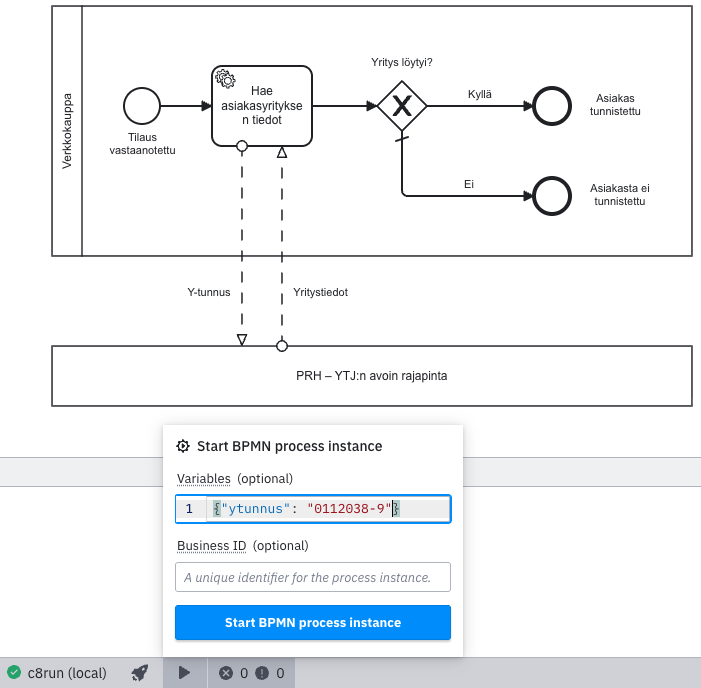
\includegraphics[keepaspectratio]{kuviot/ytunnus.png}}

}

\caption{\label{fig-ytunnus}Service Task -tehtävä}

\end{figure}%

Prosessi kytkeytyy YTJ-palveluun rajapinnan kautta ja välittää
yritystunnuksen json-muotoisena kutsuna
(kuva~\ref{fig-service_task-maarittely}).

\begin{figure}

\centering{

\pandocbounded{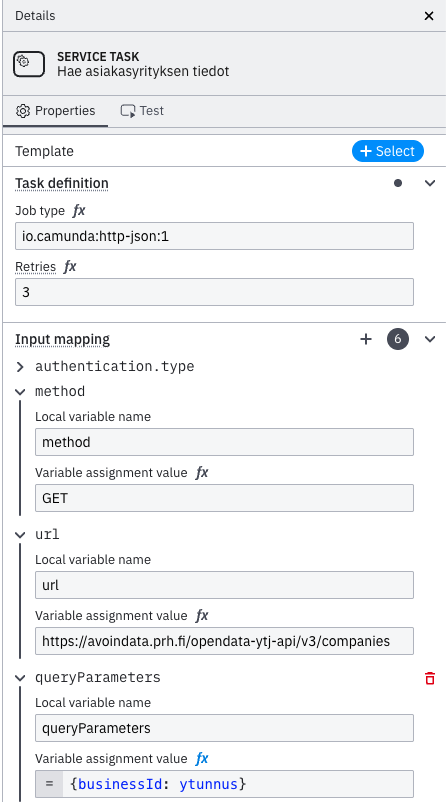
\includegraphics[keepaspectratio]{kuviot/ytunnus_service_task-maarittely.png}}

}

\caption{\label{fig-service_task-maarittely}Hae asiakasyrityksen tiedot
-tehtävän määrittelyä Camundassa}

\end{figure}%

Kun prosessi suoritetaan, se kutsuu YTJ-palvelua, joka palauttaa
yritystunnusta vastaavan yrityksen nimen
(kuva~\ref{fig-ytunnus_lopputulos}).

\begin{figure}

\centering{

\pandocbounded{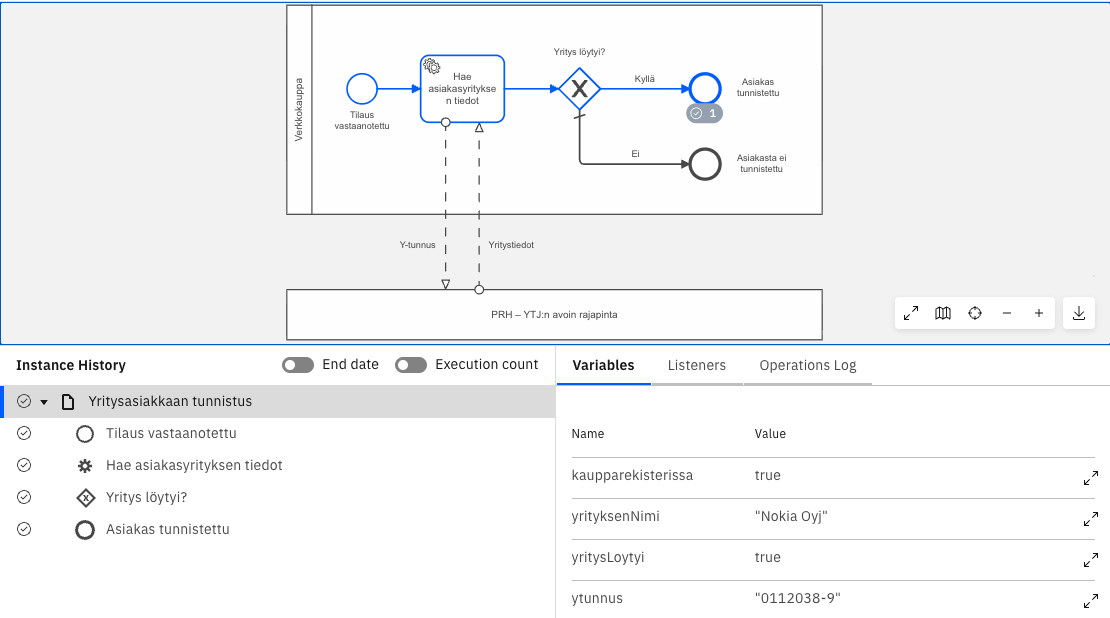
\includegraphics[keepaspectratio]{kuviot/ytunnus_lopputulos.png}}

}

\caption{\label{fig-ytunnus_lopputulos}0112038-9 on Nokian yritystunnus}

\end{figure}%

\subsubsection{Business Rule Task}\label{business-rule-task}

\emph{Business Rule Taskin} avulla voidaan suorittaa automaattista
sääntöperustaista päätöksentekoa. Päätössäännöt esitetään \emph{Decision
Model and Notation} (DMN) -muodossa, joka on standardoitu tapa mallintaa
ja esittää päätöksiä\sidenote{\footnotesize https://www.omg.org/dmn/}. DMN:n avulla
voidaan kuvata liiketoimintapäätöksiä yksiselitteisesti ja mallintaa
päätöslogiikkaa myös ei-teknisten sidosryhmien ymmärtämässä muodossa.
Erityisesti se myös mahdollistaa päätöstilanteiden automatisoimisen
osana liiketoimintaprosesseja. Lisäksi DMN:lla voidaan esittää
päätöksenteon kokonaisrakennetta (esimerkiksi mitkä päätökset
vaikuttavat toisiinsa) ja määritellä taulukkomuotoisia (\emph{Decision
Tables}) sääntökokonaisuuksia ja ehtoja päätöksentekotilanteisiin.

\begin{figure}

\centering{

\pandocbounded{\includegraphics[keepaspectratio]{index_files/mediabag/kuviot/business_rule_task.pdf}}

}

\caption{\label{fig-business_rule_task}Business Rule Taskin avulla
prosessin aikana voidaan suorittaa sääntöperusteista automaattista
päätöksentekoa}

\end{figure}%

Päätöksen tekeminen tapahtuu niin, että tehtävään menee syötteenä
joitain tietoja, joita verrataan ennalta määriteltyihin ehtoihin, joiden
perusteella päätös tehdään. Prosessimuuttujille voidaan asettaa
päätöksen mukaiset arvot ja prosessikulku etenee Business Rule Taskin
jälkeen päätöstä vastaavasti (kuva~\ref{fig-dmn-hakemus}).

\begin{figure}

\centering{

\pandocbounded{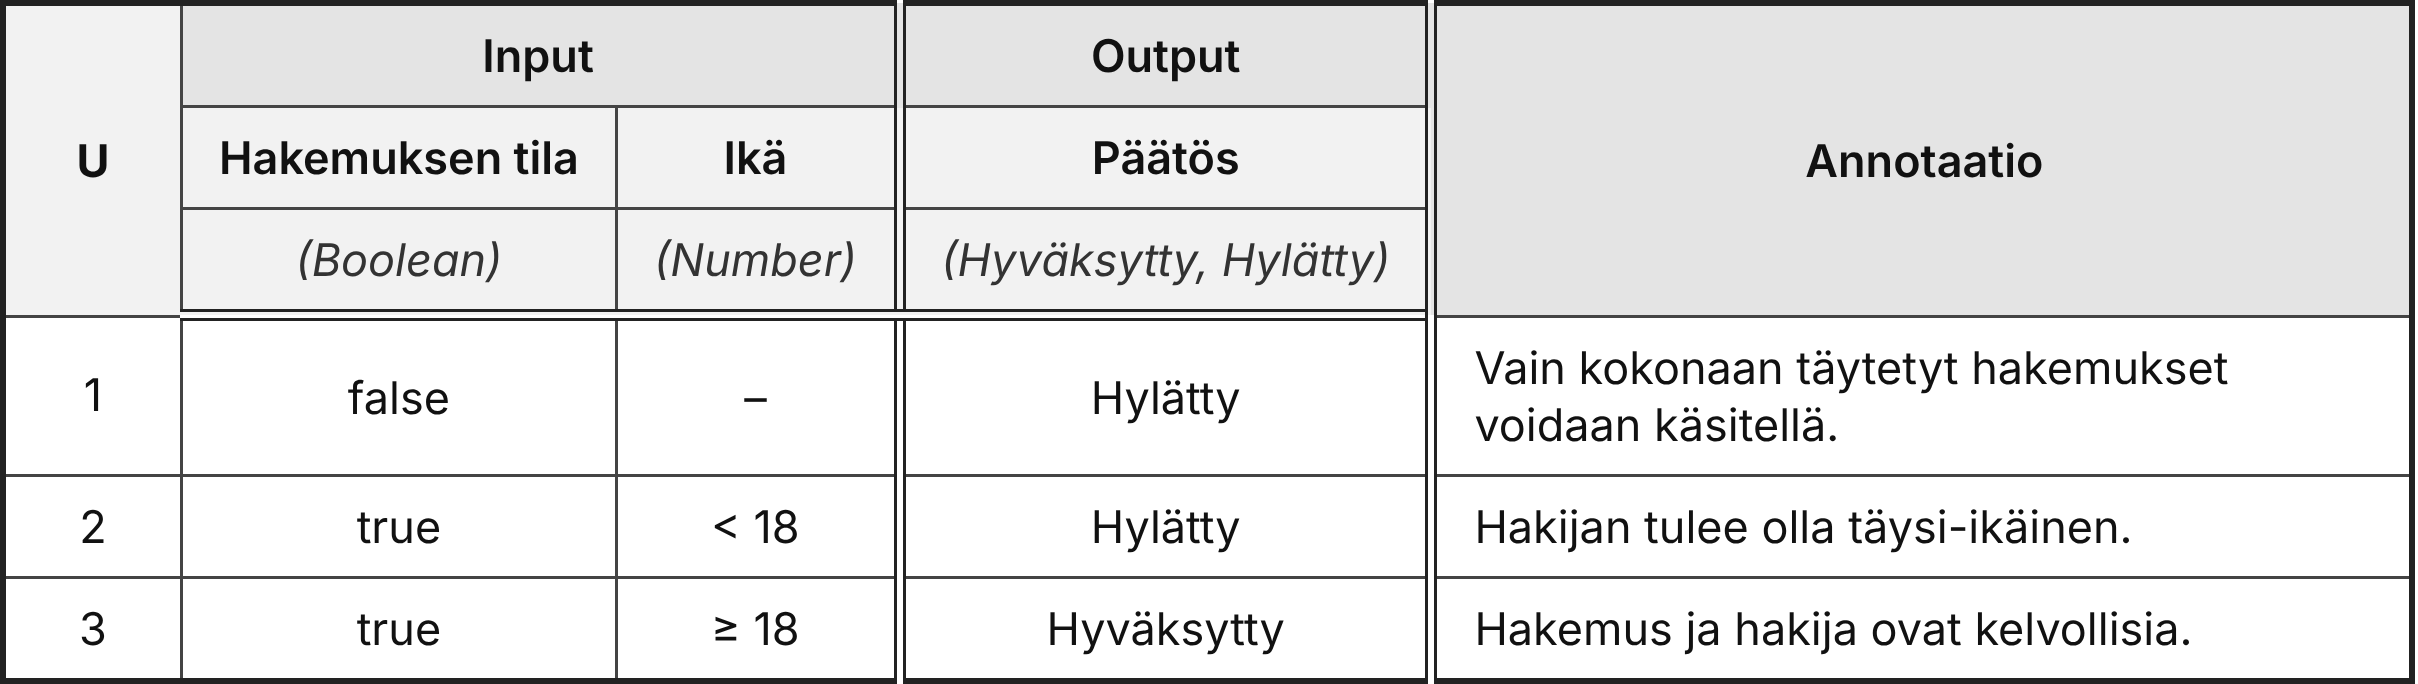
\includegraphics[keepaspectratio]{kuviot/dmn-hakemus.png}}

}

\caption{\label{fig-dmn-hakemus}Hakemuksen automaattinen käsittely}

\end{figure}%

\emph{Päätä hakemuksesta} -Business Rule Task on liitetty
\texttt{hakemuksen-paatos} -päätöstauluun, joka Camundassa voisi näyttää
seuraavalta (kuva~\ref{fig-dmn-paatostaulu}).

\begin{figure}

\centering{

\pandocbounded{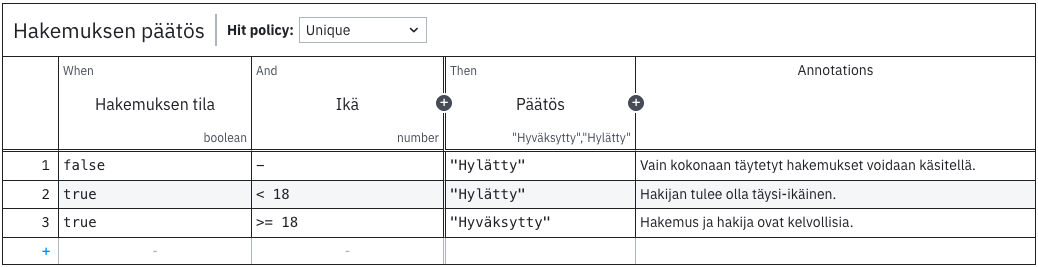
\includegraphics[keepaspectratio]{kuviot/dmn-paatostaulu.png}}

}

\caption{\label{fig-dmn-paatostaulu}Päätöstaulu hakemuksesta
päättämiseksi}

\end{figure}%

Päätöstaulua seuraten hakemus hyväksytään, kun hakemus on kokonaan
täytetty ja hakija on täysi-ikäinen. Päätöstyyppi (\emph{Hit policy})
\texttt{Unique} tarkoittaa, että päätöksen tekemiseen käytetään vain
yhtä sääntöä eivätkä päällekkäiset tai toisensa kumoavat päätökset ole
mahdollisia.

Edellinen päätös voitaisiin tietenkin rakentaa prosessikulkuun myös
valintaporttien avulla. Päätöstaulujen hyödyntäminen on kuitenkin
prosessin suorittamisen kannalta tehokkaampi tapa ja hyödyllinen
erityisesti siksi, että tietyn päätöksen logiikka voidaan tiivistää
yhteen tehtävään. Tällöin liiketoimintasääntöjen tai vaikkapa päätökseen
vaikuttavan lainsäädännön muutokset voidaan toteuttaa hallitummin yhteen
paikkaan. Päätöstaulua voitaisiin käyttää myös esimerkiksi verkkokaupan
asiakkaan kotimaan perusteella määräytyvän arvonlisäveron
määrittämiseen, jolloin ajantasaiset ALV-tiedot voidaan koota yhteen
taulukkoon.

\subsubsection{Send Task ja Receive
Task}\label{send-task-ja-receive-task}

BPMN:ssa on kaksi tehtävää prosessin aikana tapahtuvan viestinnän tai
tiedonsiirron esittämiseksi tilanteissa, joissa tietoa siirtyy prosessin
ulkopuolelle tai tulee sisään: \emph{Send Task} ja \emph{Receive Task}
(kuva~\ref{fig-send_receive_tasks}). Niiden avulla voidaan esittää sekä
synkronista että asynkronista viestinvaihtoa muiden prosessien,
toimijoiden tai järjestelmien kanssa.

Send Task tarkoittaa, että tehtävä lähettää viestin jollekin toiselle
toimijalle tai järjestelmälle. Tehtävän suorittamisen jälkeen prosessi
jatkuu välittömästi eteenpäin, joten tarvittaessa prosessiin tulee
määritellä, mikäli sen halutaan odottavan vastauksen saapumista. Viesti
voi olla esimerkiksi sähköposti, lasku, tilauspyyntö tai vaikkapa
API-kutsu. Tosin oikeaoppisempaa viimeisen toteuttamiseksi on käyttää
Service Task -tehtävää.

Receive Task -tehtävässä prosessi puolestaan pysähtyy odottamaan
saapuvaa viestiä ennen eteenpäin jatkamista. Tätä tehtävää käytetään
luonnollisesti silloin, kun prosessin eteneminen tarvitsee jonkin
signaalin, vastauksen tai muun tiedon.

\begin{figure}

\centering{

\pandocbounded{\includegraphics[keepaspectratio]{index_files/mediabag/kuviot/send_receive_tasks.pdf}}

}

\caption{\label{fig-send_receive_tasks}Send Task ja Receive Task
lähettävät ja vastaanottavat viestejä}

\end{figure}%

Send Task merkitään tummalla kirjekuorella ja Receive Task valkoisella.

\subsubsection{Call Activity}\label{call-activity}

\emph{Call Activity} ei oikeastaan ole tehtävä, vaan se on viittaus
johonkin toiseen prosessiin tai tehtävään, joka kutsutaan suorittamaan
oma osuutensa osana prosessikulkua. Sen avulla prosessin rakennetta
voidaan modularisoida ja toisaalta se mahdollistaa prosessien
uudelleenkäytön. Sen sijaan, että samoja prosessirakenteita
monistettaisiin useaan paikkaan, voidaan niihin viitata kertaalleen
määriteltyinä ja hallinnoituina kokonaisuuksina. Tällöin vältytään myös
siltä, että jonkin useissa yhteyksissä toistuvan toimintosarjan
muuttuessa nämä muutokset tulisi toteuttaa kaikkiin samaa toimintosarjaa
toteuttaviin prosesseihin.

Seuraavassa esimerkissä (kuva~\ref{fig-call_activity}) asiakkaan tulee
tunnistautua maksupyynnön vastaanottamisen jälkeen. Tunnistautumista
varten kutsutaan Call Activityllä \emph{Tunnista käyttäjä} prosessia
\texttt{kaksivaiheinen-tunnistautuminen}, jolle propagoidaan -- eli
viedään -- kutsuvan prosessin kaikkien muuttujien arvot.

\begin{figure}

\centering{

\pandocbounded{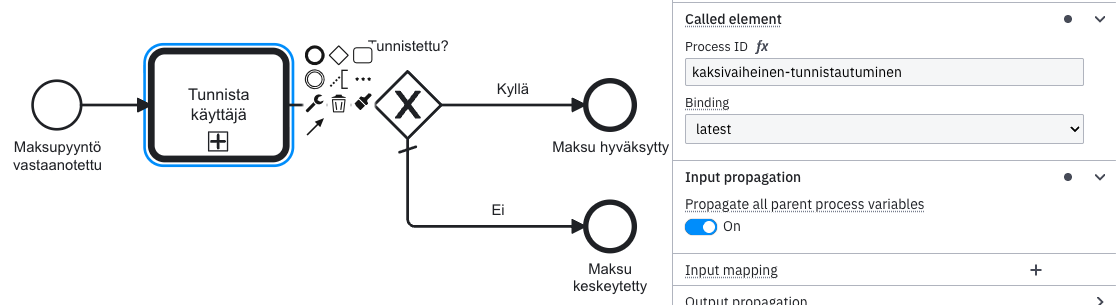
\includegraphics[keepaspectratio]{kuviot/call_activity.png}}

}

\caption{\label{fig-call_activity}Tunnistautumista varten kutsutaan Call
Activityllä erillistä prosessia}

\end{figure}%

Propagoinnin sijaan muuttujien välittämisessä voidaan käyttää myös
määriteltyjä input- ja output-parametreja. Ne siirtyvät Call Activityllä
kutsuttavaan prosessiin ja siitä takaisin. Kutsuva prosessi saa
vastauksena ainoastaan paluumuuttujan arvon, eikä sen tarvitse päästä
näkemään kutsutun prosessin sisälle, ja toisaalta kutsuttavalle
prosessille annetaan vain tiedot, jotka sen tarvitsee nähdä.

Edellinen Call Activityn kutsuma tunnistautumisprosessi voisi näyttää
seuraavalta (kuva~\ref{fig-kaksivaiheinen-tunnistautuminen}).

\begin{figure}

\centering{

\pandocbounded{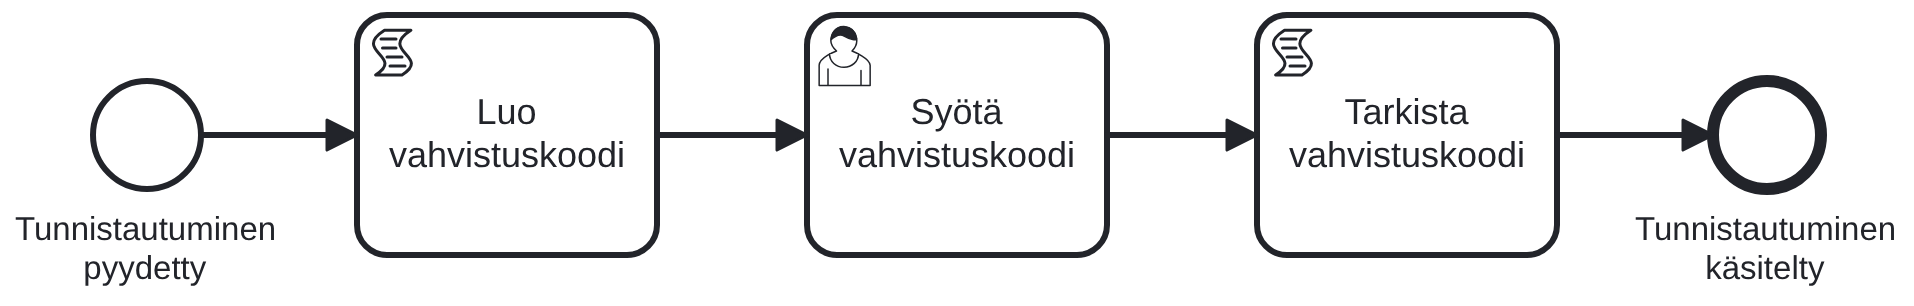
\includegraphics[keepaspectratio]{kuviot/kaksivaiheinen-tunnistautuminen.png}}

}

\caption{\label{fig-kaksivaiheinen-tunnistautuminen}Kaksivaiheisen
tunnistautumisen prosessi}

\end{figure}%

Samaa tunnistautumisprosessia voitaisiin kutsua kirjautumisen, salasanan
vaihdon tai vaikkapa tilitietojen muuttamisen yhteydessä. Jos
tunnistautumistapa muuttuu, muutos tarvitsee tehdä vain yhteen paikkaan.

Call Activityllä kutsuttava prosessi on myös suoritettavissa useana
instanssina, eli se on esimerkiksi mahdollista suorittaa jokaiselle
asiakkaalle erikseen saman prosessikulun aikana.

\subsubsection{Sub Process}\label{sub-process}

Call Activityn tavoin myös \emph{Sub Process} ei ole prosessikulun
aikana suoritettava yksittäinen tehtävä, vaan nimensä mukaisesti
aliprosessi, joka koostuu sarjasta tehtäviä. Sub Process merkitään
vastaavalla symbolilla kuin Call Activity, mutta sen reunaviiva on ohut.
(kuva~\ref{fig-sub_process_kiinni})

\begin{figure}

\centering{

\pandocbounded{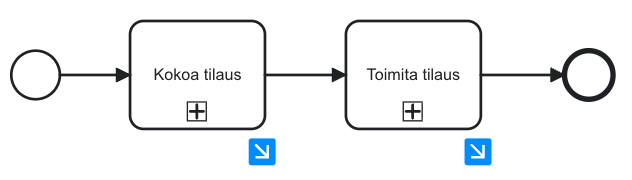
\includegraphics[keepaspectratio]{kuviot/sub_process_kiinni.png}}

}

\caption{\label{fig-sub_process_kiinni}Prosessikulku, jossa on kaksi
aliprosessia}

\end{figure}%

Jokaisen Sub Process -elementin alla on siis tehtävistä koostuva oma
prosessikulkunsa, jolle tulee myös määritellä aloitus- ja lopetuspisteet
(kuva~\ref{fig-sub_process_auki}).

\begin{figure}

\centering{

\pandocbounded{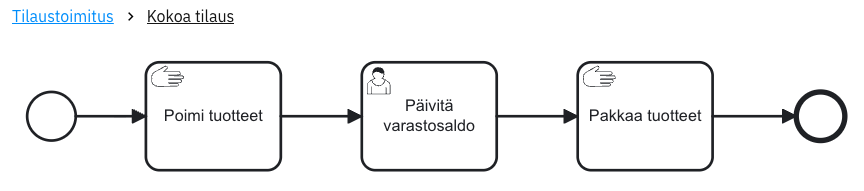
\includegraphics[keepaspectratio]{kuviot/sub_process_auki.png}}

}

\caption{\label{fig-sub_process_auki}Kokoa tilaus -aliprosessi avattuna}

\end{figure}%

Aliprosessi on osa pääprosessia ja sitä voidaan käyttää jäsentämään tai
yksinkertaistamaan prosessikaaviota. Siten se mahdollistaa prosessin
jakamisen osiin, jotka voidaan haluttaessa piilottaa korkeamman tason
näkymästä. Call Activityn ja Sub Processin eroja on koottu seuraavaan
taulukkoon (Taulukko~\ref{tbl-call-activity-sub-process}).

\begin{longtable}[]{@{}
  >{\raggedright\arraybackslash}p{(\linewidth - 2\tabcolsep) * \real{0.5000}}
  >{\raggedright\arraybackslash}p{(\linewidth - 2\tabcolsep) * \real{0.5000}}@{}}
\caption{Call Activityn ja Sub Processin
erot}\label{tbl-call-activity-sub-process}\tabularnewline
\toprule\noalign{}
\begin{minipage}[b]{\linewidth}\raggedright
Call Activity
\end{minipage} & \begin{minipage}[b]{\linewidth}\raggedright
Sub Process
\end{minipage} \\
\midrule\noalign{}
\endfirsthead
\toprule\noalign{}
\begin{minipage}[b]{\linewidth}\raggedright
Call Activity
\end{minipage} & \begin{minipage}[b]{\linewidth}\raggedright
Sub Process
\end{minipage} \\
\midrule\noalign{}
\endhead
\bottomrule\noalign{}
\endlastfoot
Kohde määritellään aina erillisessä prosessikaaviossa. & Sub Process
määritellään samassa prosessikaaviossa pääprosessin kanssa. \\
Kohdetta voidaan käyttää useissa prosesseissa, joista sitä kutsutaan. &
Sub Processia voidaan käyttää ainoastaan sen pääprosessissa. \\
Kutsuttaessa Call Activityä, input- ja output-parametrit tulee
määritellä eksplisiittisesti\sidenotemark{}. & Sub
Process perii viestivirrat pääprosessilta, joten sillä on käytettävissä
kaikki prosessissa oleva tieto ilman erillistä määrittelyä. \\
Call Activity esitetään aina tiivistettynä eli yhdellä
tehtäväelementillä. & Sub Process voidaan esittää tiivistettynä tai se
voidaan esittää avattuna aliprosessin kulun tarkastelua varten. \\
\end{longtable}\sidenotetext{Asia on näin BPMN-standardin
  tasolla. Esimerkeissä käytettävässä Camunda 8:ssa kutsuttu prosessi
  saa kaikki kutsujan muuttujat (Propagate all parent process variables)
  ja palauttaa kaikki omansa, ellei siirtoa rajata erikseen.}


\subsubsection{Loop, Parallel Multi-instance, Sequential Multi-instance
ja
Ad-hoc}\label{loop-parallel-multi-instance-sequential-multi-instance-ja-ad-hoc}

BPMN tarjoaa keinoja mallintaa tehtäville sekä aliprosesseille toistuvia
tai vaihtoehtoisia käyttäytymismalleja: \emph{Loop}, \emph{Parallel
Multi-Instance}, \emph{Sequential Multi-Instance} ja \emph{Ad-hoc}.

Loop (kuva~\ref{fig-loop}) toimii kuten \texttt{do-while}-rakenne
ohjelmointikielissä ja tehtävää suoritetaan niin kaun kuin ehto on tosi.
Ehto tarkastetaan tehtävän suorittamisen jälkeen tai haluttaessa jo
ennen ensimmäistä suorituskertaa (\texttt{testBefore}). Silmukassa
toistuvalle tehtävälle voidaan asettaa myös toistokertojen enimmäismäärä
(\texttt{loopMaximum}).

\begin{figure}

\centering{

\pandocbounded{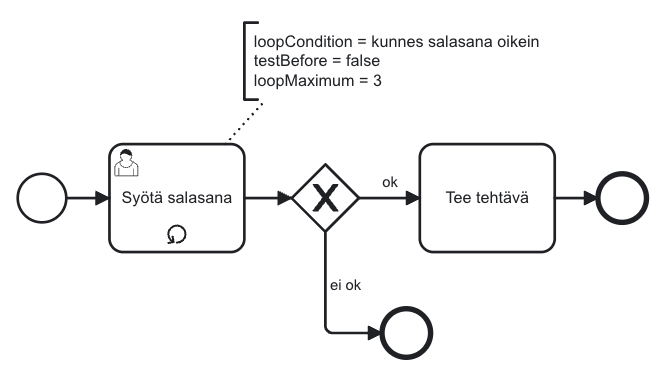
\includegraphics[keepaspectratio]{kuviot/loop.png}}

}

\caption{\label{fig-loop}Ehtoperusteisesti toistettava Loop-tehtävä}

\end{figure}%

Parallel Multi-Instance käynnistää tehtävästä useita rinnakkain
suoritettavia toteutuksia eli instansseja. Syötteenä tällaiselle
tehtävälle tarvitaan tyypillisesti lista tai joukko, jonka alkiot
toimivat syötteinä kullekin instanssille.

Sequential Multi-Instance puolestaan käynnistää tehtävät peräkkäisinä.
Seuraava instanssi käynnistyy, kun edellinen on valmis.
(kuva~\ref{fig-multi_instance}) Molemmissa tapauksissa prosessissa
siirrytään eteenpäin sitten, kun kaikki instanssit on suoritettu. Koska
nämä tehtävätyypit käyvät läpi joukon alkioita
\texttt{foreach}-rakenteen tyyliin, ne eivät ole Loopin kaltaisia
silmukkarakenteita.

\begin{figure}

\centering{

\pandocbounded{\includegraphics[keepaspectratio]{index_files/mediabag/kuviot/multi_instance.pdf}}

}

\caption{\label{fig-multi_instance}Tehtävän toteutus rinnakkaisina
instansseina (Parallel Multi-instance) ja peräkkäisinä instansseina
(Sequential Multi-instance)}

\end{figure}%

Seuraava esimerkki (kuva~\ref{fig-multi_esim1}) kuvaa tilannetta, jossa
asiakas asioi myymälässä. Kukin hänen tilaamansa tuote poimitaan
varaston hyllyltä, yksi kerrallaan ja peräkkäisessä järjestyksessä.
Tämän jälkeen asiakkaalta peritään maksu. Maksua penätään asiakkaalta
tarvittaessa useampaan kertaan, ennen kuin tuotteet luovutetaan. Jos
asiakas ei maksa viidennelläkään pyynnöllä (loopMaximum = 5), ei
tuotteita luovuteta.

\begin{figure}

\centering{

\pandocbounded{\includegraphics[keepaspectratio]{index_files/mediabag/kuviot/multi_esim1.pdf}}

}

\caption{\label{fig-multi_esim1}Tehtävän toistaminen peräkkäin
(tuotteiden kerääminen) ja kunnes ehto täyttyy (maksusuoritus tehty)}

\end{figure}%

Toisen esimerkin (kuva~\ref{fig-multi_esim2}) tilaus liittyy
digitaalisiin tuotteisiin, joihin käyttäjälle annetaan maksun jälkeen
käyttöoikeudet. Kaikki käyttöoikeudet voidaan luovuttaa kerralla, joten
tehtävän instanssit voidaan suorittaa rinnakkain. Prosessi päättyy ilman
käyttöoikeuksien luovuttamista, mikäli asiakas ei ole maksanut
tilaustaan kahden maksumuistutuksen jälkeen.

\begin{figure}

\centering{

\pandocbounded{\includegraphics[keepaspectratio]{index_files/mediabag/kuviot/multi_esim2.pdf}}

}

\caption{\label{fig-multi_esim2}Usean tehtäväinstanssin suorittaminen
rinnakkain}

\end{figure}%

Ad-hoc -prosessi tai -aliprosessi on BPMN-kielen villi kortti
(kuva~\ref{fig-ad-hoc}).

\begin{figure}

\centering{

\pandocbounded{\includegraphics[keepaspectratio]{index_files/mediabag/kuviot/ad-hoc.pdf}}

}

\caption{\label{fig-ad-hoc}Ad-hoc -aliprosessi}

\end{figure}%

Sen avulla voidaan esittää tehtäväsarjoja, joiden suoritusjärjestys ei
ole ennalta määritelty. Ad-hoc -prosessiin kuuluvat tehtävät voidaan
suorittaa kokonaan tai osittain, vapaassa järjestyksessä tai vaikka
rinnakkain (kuva~\ref{fig-ad-hoc_auki}). Näin ollen ad-hoc -prosessille
ei myöskään määritellä prosessikulkua. Ad-hoc -tyyppinen prosessi
merkitään tilde-merkillä (\textasciitilde), jolla matematiikassa
ilmaistaan approksimaatiota.

\begin{figure}

\centering{

\pandocbounded{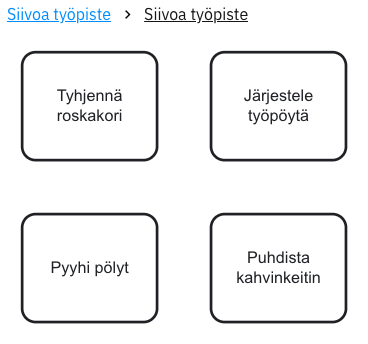
\includegraphics[keepaspectratio]{kuviot/ad-hoc_auki.png}}

}

\caption{\label{fig-ad-hoc_auki}Siivoa työpiste -ad-hoc-prosessin
tehtävät}

\end{figure}%

\subsection{Tapahtumat}\label{tapahtumat}

Siinä missä edellä käsitellyt tehtävät kuvaavat prosessin aikana
suoritettavaa tekemistä, tapahtumat (\emph{Event}) kuvaavat asioita,
jotka `tapahtuvat' prosessin aikana. BPMN:ssa tapahtumia on kolmea
päätyyppiä: \emph{Start Event} (aloitustapahtuma), \emph{Intermediate
Event} (välitapahtuma) sekä \emph{End Event} (lopetustapahtuma).
Tapahtumat voivat siis käynnistää, keskeyttää tai päättää prosessin, tai
tapahtua prosessin aikana. Kullakin päätyypillä on alityyppejä, jotka
käsitellään seuraavissa alaluvuissa. BPMN:n graafisessa notaatiossa
tapahtumat esitetään ympyrällä (kuva~\ref{fig-events}). Start Event
-tyyppisissä tapahtumissa ympyrän kehä piirretään ohuella viivalla, End
Event -tapahtumissa paksulla viivalla ja Intermediate Event
-tapahtumissa kaksoisviivalla.

\begin{figure}

\centering{

\pandocbounded{
\includegraphics[keepaspectratio]{kuviot/events.png}}

}

\caption{\label{fig-events}Tapahtumien päätyypit ja niissä käytetty
graafinen notaatio: Start Event, Intermediate Event ja End Event}

\end{figure}%

Jotkin intermediate-tyyppisistä tapahtumista voidaan myös liittää
tehtävään, jolloin niitä kutsutaan nimellä \emph{Boundary Event}.
Tällainen rajatapahtuma voi olla keskeyttävä (\emph{interrupting}) tai
ei-keskeyttävä (\emph{non-interrupting}), jolloin se esitetään
kaksoiskatkoviivalla (kuva~\ref{fig-boundaryt}).

\begin{figure}

\centering{

\pandocbounded{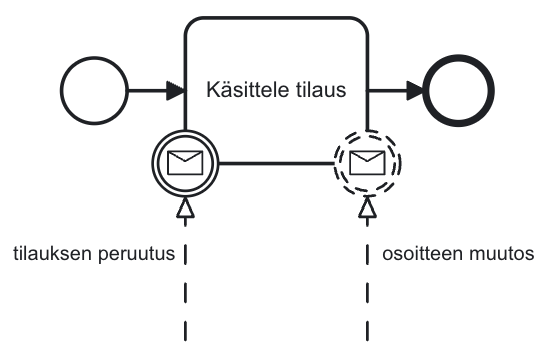
\includegraphics[keepaspectratio]{kuviot/boundaryt.png}}

}

\caption{\label{fig-boundaryt}Keskeyttävä (Interrupting) ja
ei-keskeyttävä (Non-interrupting) Boundary Event}

\end{figure}%

Mikäli tilauksen käsittelyn aikana vastaanotettaisiin ilmoitus tilauksen
peruutuksesta, tehtävän suorittaminen lopetettaisiin. Vastaavasti
asiakkaan ilmoittama tieto osoitteen muutoksesta ei keskeyttäisi
tilauksen käsittelyä, vaan johtaisi tilauksen osoitetiedon
päivittämiseen.

Keskeyttävän ja ei-keskeyttävän tapahtuman toiminnalliset erot on
esitetty seuraavassa taulukossa
(Taulukko~\ref{tbl-keskeyttava-tapahtuma}).

\begin{longtable}[]{@{}
  >{\raggedright\arraybackslash}p{(\linewidth - 4\tabcolsep) * \real{0.3333}}
  >{\raggedright\arraybackslash}p{(\linewidth - 4\tabcolsep) * \real{0.3333}}
  >{\raggedright\arraybackslash}p{(\linewidth - 4\tabcolsep) * \real{0.3333}}@{}}
\caption{Keskeyttävän ja ei-keskeyttävän tapahtuman
erot}\label{tbl-keskeyttava-tapahtuma}\tabularnewline
\toprule\noalign{}
\begin{minipage}[b]{\linewidth}\raggedright
\end{minipage} & \begin{minipage}[b]{\linewidth}\raggedright
Keskeyttävä tapahtuma
\end{minipage} & \begin{minipage}[b]{\linewidth}\raggedright
Ei-keskeyttävä tapahtuma
\end{minipage} \\
\midrule\noalign{}
\endfirsthead
\toprule\noalign{}
\begin{minipage}[b]{\linewidth}\raggedright
\end{minipage} & \begin{minipage}[b]{\linewidth}\raggedright
Keskeyttävä tapahtuma
\end{minipage} & \begin{minipage}[b]{\linewidth}\raggedright
Ei-keskeyttävä tapahtuma
\end{minipage} \\
\midrule\noalign{}
\endhead
\bottomrule\noalign{}
\endlastfoot
Keskeyttääkö nykyisen tehtävän / prosessin? & Kyllä & Ei \\
Jatkuuko alkuperäinen tehtävä? & Ei, se keskeytetään & Kyllä, se jatkuu
normaalisti loppuun saakka \\
Käynnistääkö uuden polun? & Kyllä & Kyllä \\
Käyttötarkoitus & Kriittinen tapahtuma, kuten virhe tai aikakatkaisu &
Lisälogiikka, ilmoitukset, monitorointi \\
\end{longtable}

Seuraavassa kuviossa (kuva~\ref{fig-eventteja}) on tilauskäsittelyn
prosessimalli, jossa on Start Event -aloitustapahtuma, sitä seuraava
tehtävä \emph{Kerää tilauksen tuotteet}. Tähän liittyy Non-interrupting
Boundary Event, joka aktivoi tehtävän \emph{Ilmoita viivästyksestä},
mikäli kaksi vuorokautta ehtii kulua ennen kuin tuotteet on kerätty.
Tämän jälkeen siirrytään tehtävään \emph{Toimita tilaus}, jonka jälkeen
prosessi päättyy End Eventiin.

\begin{figure}

\centering{

\pandocbounded{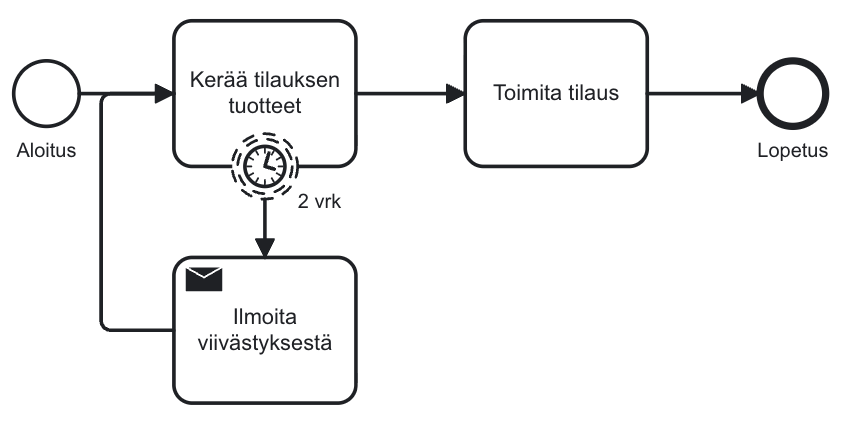
\includegraphics[keepaspectratio]{kuviot/eventteja.png}}

}

\caption{\label{fig-eventteja}Start Event, Boundary Event ja End Event}

\end{figure}%

Seuraavassa esimerkissä (kuva~\ref{fig-eventteja2}) esiintyy myös
Terminate Event. Se voidaan mieltää End Eventin voimakkaammaksi
versioksi. Prosessin jonkin haaran päätyessä Terminate Eventiin, koko
prosessi lopetetaan riippumatta siitä, missä vaiheessa sen muut haarat
ovat. Mikäli tilaus peruutetaan, kaikki prosessiin liittyvä toiminta
lopetetaan.

\begin{figure}

\centering{

\pandocbounded{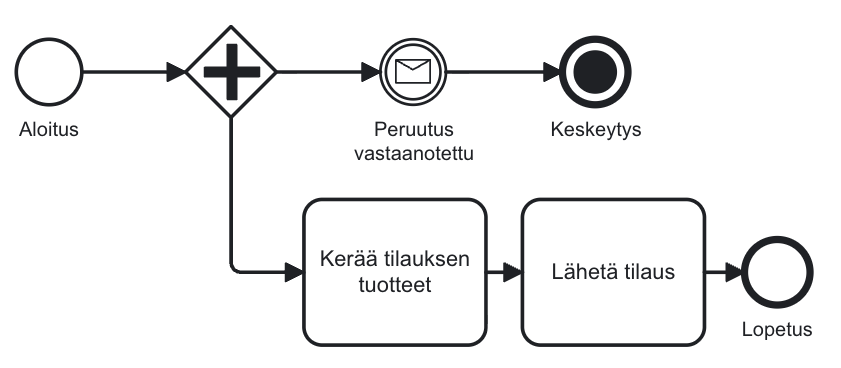
\includegraphics[keepaspectratio]{kuviot/eventteja2.png}}

}

\caption{\label{fig-eventteja2}Terminate Event}

\end{figure}%

\subsubsection{Message Event}\label{message-event}

Message Event -viestitapahtumia on muutama erilainen. \emph{Message
Start Event} on prosessin käynnistävä tapahtuma. Prosessi käynnistyy,
kun se vastaanottaa viestin toiselta prosessilta tai vaikkapa ulkoiselta
järjestelmältä. Viesti voi olla esimerkiksi puhelinsoitto tai
verkkokaupasta tuleva tilaus, joka käynnistäisi
tilauskäsittelyprosessin.

Jo edellä nähdyn \emph{Message Intermediate Event} -tapahtuman
(kuva~\ref{fig-eventteja2}) avulla voidaan esittää tilanne, jossa
prosessin jokin tehtävä on valmis vastaanottamaan viestin, johon se
reagoi, mikäli viesti saapuu.

Seuraavassa esimerkissä (kuva~\ref{fig-eventteja3}) Message Start Event
käynnistää prosessin saadessaan viestin tehdystä tilauksesta.
Ensimmäisessä tehtävässä asiakkaalta ruvetaan keräämään maksua. Tähän
tehtävään liittyy myös \emph{Message Boundary Event} eli tieto
tapahtumasta, jossa asiakas onkin perunut tilauksensa. Jos prosessia
luetaan tarkkaavaisesti, huomataan, että viesti tilauksen perumisesta
voi saapua sinä aikana, kun maksun kerääminen on vielä käynnissä. Mikäli
prosessi siirtyy \emph{Lähetä tilaus} -tehtävään, ei tilauksen peruminen
enää voi johtaa prosessin päättymiseen. Prosessia suunniteltaessa tulee
tietenkin huomioida, että mikäli asiakas voi perua tilauksen vielä
maksamisen jälkeenkin (minkä etämyyntiä koskevan lainsäädännön mukaan
täytyykin Suomessa olla mahdollista), ei prosessi voi ainoastaan päättyä
perumisviestin vastaanottavan tapahtuman jälkeen, vaan prosessin tulee
huolehtia muun muassa maksun palauttamisesta asiakkaalle.
Esimerkkiprosessimme päättyy \emph{Lähetä tilaus} -tehtävää seuraavaan
\emph{Message End Event} -tapahtumaan, joka voisi prosessin lopuksi
lähettää asiakkaalle tiedon siitä, että hänen tilauksensa on jätetty
kuljetettavaksi.

\begin{figure}

\centering{

\pandocbounded{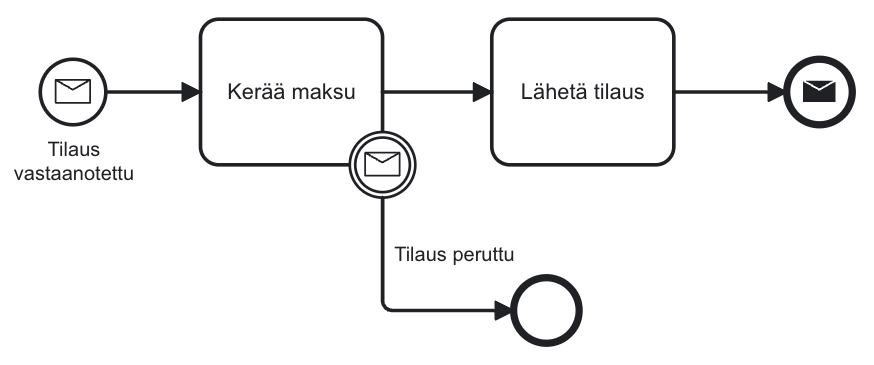
\includegraphics[keepaspectratio]{kuviot/eventteja3.png}}

}

\caption{\label{fig-eventteja3}Message Start Event, Message Intermediate
Boundary Event ja Message End Event}

\end{figure}%

Edellä todettiin, että Boundary Eventit voivat olla keskeyttäviä tai
ei-keskeyttäviä. Yllä olevan prosessin johonkin tehtävään voisi liittyä
esimerkiksi ei-keskeyttävä Message Boundary Event, joka ottaisi vastaan
asiakkaan tilaukseensa mahdollisesti tekemän muutoksen, kuten
esimerkiksi tilaukseen lisätyt tuotteet. Tällainen tapahtuma aloittaisi
prosessissa uuden polun, jonka tehtävät päivittäisivät tilausta
vastaavalla tavalla. Tällaista prosessia suunniteltaessa tietenkin olisi
harkittava, kuinka paljon asiakkaan halutaan sallia tilaustaan säätää,
jotta toiminta on järkevää liiketoimintaprosessien sujuvuuden ja
tehokkuuden kannalta, ja toisaalta sujuvan ja myönteisen
asiakaskokemuksen kannalta.

\subsubsection{Conditional Event}\label{conditional-event}

\emph{Conditional Event} eli ehdollinen tapahtuma voi olla prosessin
ehdollisesti käynnistävä Conditional Start Event tai prosessin aikana
tapahtuva \emph{Conditional Boundary Event} tai \emph{Conditional
Intermediate Catch Event} (kuva~\ref{fig-conditional}).

\begin{figure}

\centering{

\pandocbounded{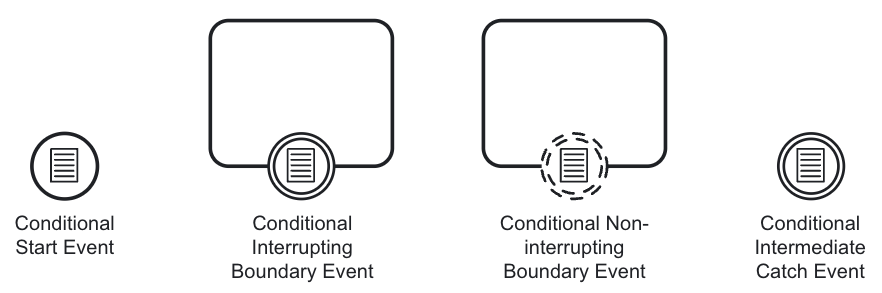
\includegraphics[keepaspectratio]{kuviot/conditional.png}}

}

\caption{\label{fig-conditional}Erityyppisiä ehdollisia tapahtumia}

\end{figure}%

Ehdollinen aloitustapahtuma siis käynnistää prosessin tietyn ennalta
määritellyn ja tarvittaessa monimutkaisenkin ehdon täyttyessä
(kuva~\ref{fig-cond_esim}). Conditional Boundary Event, eli ehdollinen
rajatapahtuma, voi olla tyypiltään keskeyttävä tai ei-keskeyttävä. Ehdon
täyttyessä tehtävä voi käynnistää prosessiin uuden haaran. Conditional
Intermediate Catch Event puolestaan pysäyttää prosessin, kunnes
määritelty ehto muuttuu todeksi, jonka jälkeen eteneminen jatkuu.

\begin{figure}

\centering{

\pandocbounded{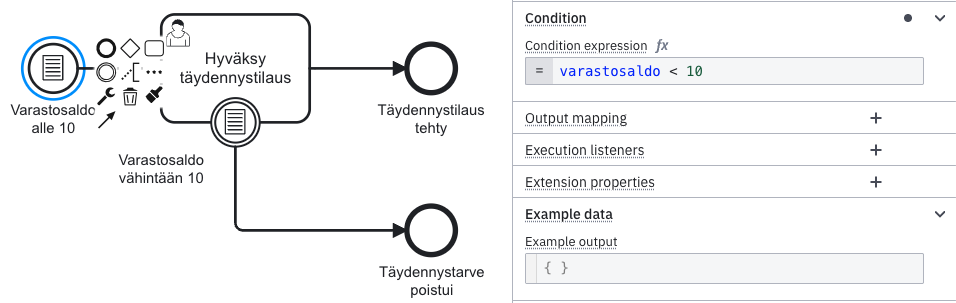
\includegraphics[keepaspectratio]{kuviot/cond_esim.png}}

}

\caption{\label{fig-cond_esim}Esimerkki yksinkertaisesta Conditional
Start Eventin aloitusehdosta}

\end{figure}%

Tässä vaiheessa saattaa ajatella, että mihin tällaisia tapahtumatyyppejä
tarvitaan. Eikö saman asian voi esittää ja saman toiminnallisuuden
toteuttaa joitain muita elementtityyppejä -- kuten viestejä -- käyttäen?
Vastaus ainakin useimmissa tapauksissa on, että kyllä voi. Ehdollisten
tapahtumien etu viesteihin perustuvaan kommunikointiin verrattuna on
löyhäkytkentäisyydessä (Loose Coupling).

Ehdolliset tapahtumat mahdollistavat loogisten ehtojen varassa
toimimisen, sen sijaan, että prosessiin tarvitsee rakentaa tiukkoja,
rajapintojen ja viestimuotojen tuntemista edellyttäviä kytkentöjä. Ehto
voi olla loogisesti johdettu tai vaikkapa tietovarastosta saatava tieto
siitä, että tilauksen maksu on suoritettu. Tämä sen sijaan, että
prosessilla tulisi olla valmiudet kytkeytyä kaikkiin nykyisiin ja
mahdollisiin tuleviin vaihtoehtoisiin maksujärjestelmiin sekä kyetä
tulkitsemaan ja ymmärtämään niistä saapuvat kuittausviestit.
Järjestelmiä ja muita teknisiä ratkaisuja toteutettaessa
löyhäkytkentäisyys on yleisesti hyvänä pidetty suunnitteluperiaate.
Täytyy kuitenkin muistaa, että jos prosessi halutaan rakentaa pelkästään
loogisen tason ehdoille ja päätöksille\sidenote{\footnotesize Tällöin voitaisiin ehkä
  puhua myös ''liiketoiminnan ymmärtämästä kielestä''.}, ja siten
mahdollisimman riippumattomaksi sitä ympäröivistä järjestelmistä ja
teknologioista, täytyy vaiva kuitenkin nähdä jossain muualla. Kehittäjä
joutuu todennäköisesti tekemään töitä sen eteen, että prosessin
ehdolliselle tapahtumalle saadaan tietovarastosta tai eri pankkien
maksurajapinnoista loogisen tason tieto siitä, että
\texttt{maksu\ ==\ ok}.

\subsubsection{Timer Event}\label{timer-event}

\emph{Timer Event}it eli ajastintapahtumat (kuva~\ref{fig-timer})
liittyvät ajastettuihin ja aikaan sidottuihin tapahtumiin. Niiden avulla
voidaan ilmaista esimerkiksi viivettä, ajoituksia tai jollain
aikavälillä toistuvia tapahtumia.

\emph{Timer Start Event} määrittelee, että prosessi käynnistyy jonkin
aikamääreen perusteella, esimerkiksi joka arkipäivä kello kahdeksan.
\emph{Timer Intermediate Catch Event} viivästyttää prosessin etenemistä
tietyn ajanjakson kerran -- prosessi voidaan siis määrätä odottamaan.
\emph{Timer Boundary Event} puolestaan liitetään johonkin tehtävään ja
sen avulla voidaan aloittaa toinen haara, mikäli alkuperäisen
aktiviteetin suorittaminen kestää liian kauan. Tämäkin tapahtuma voidaan
määritellä joko keskeyttäväksi tai ei-keskeyttäväksi.

\begin{figure}

\centering{

\pandocbounded{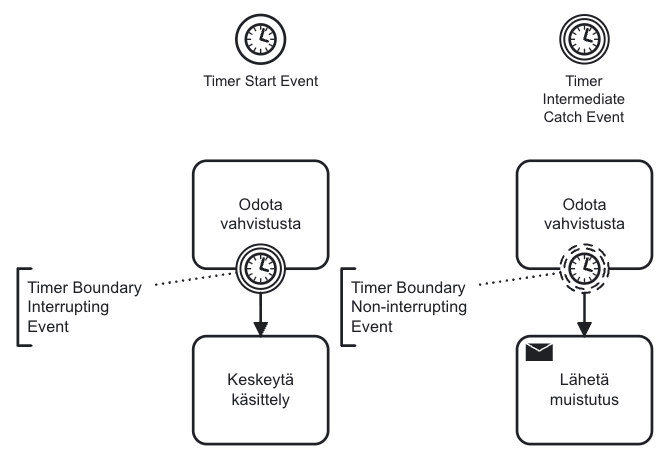
\includegraphics[keepaspectratio]{kuviot/timer.png}}

}

\caption{\label{fig-timer}Erilaisia Timer-tapahtumia}

\end{figure}%

Seuraavassa kuviossa (kuva~\ref{fig-timer_esim}) on muutama esimerkki
ajastintapahtumien käytöstä.

\begin{figure}

\centering{

\pandocbounded{\includegraphics[keepaspectratio]{index_files/mediabag/kuviot/timer_esim.pdf}}

}

\caption{\label{fig-timer_esim}Esimerkkejä Timer-tapahtuman käytöstä}

\end{figure}%

Edellä ajastintapahtumiin liittyvät aikamääreet on esitetty
yleistajuisesti. Taustalla BPMN kuitenkin käyttää ajanmäärittelyssä ISO
8601 -standardia. Seuraavassa on muutama esimerkki tämän standardin
mukaisesta aikamääreiden esittämisestä.

\emph{Fixed Date} -muotoa voidaan käyttää, kun prosessin tai tapahtuman
halutaan alkavan tiettynä ajanhetkenä. Fixed Date esitetään muodossa:

\begin{Shaded}
\begin{Highlighting}[]
\NormalTok{YYYY{-}MM{-}DDTHH:MM:SS}
\end{Highlighting}
\end{Shaded}

eli esimerkiksi \texttt{2027-03-24T08:15:00}, mikä tarkoittaa vuoden
2027 maaliskuun 24. päivää ja kellonaikaa 8:15. Aikavyöhyke ilmaistaan
liittämällä litanian perään ajan ero UTC-aikaan. Suomen normaaliaika on
kaksi tuntia edellä koordinoitua yleisaikaa, joten edellinen aikamääre
Suomen talviajassa olisi siis:

\begin{Shaded}
\begin{Highlighting}[]
\NormalTok{2027{-}03{-}24T08:15:00+02:00}
\end{Highlighting}
\end{Shaded}

\emph{Cyclen} avulla voidaan esittää toistuva ajankohta seuraavassa
muodossa, eli toistokertojen määrä, aloitusaika, toistoväli:

\begin{Shaded}
\begin{Highlighting}[]
\NormalTok{R/StartTime/Duration}
\end{Highlighting}
\end{Shaded}

Mikäli aloitusaikaa ei ilmoiteta, toistuva aika määrittyy tehtävän
ensimmäisen kohtaamisen perusteella. Mikäli toistokertoja ei määritellä,
toistoja tehdään loputtomasti. Loputtomiin kerran päivässä toistuva
tapahtuma ilmaistaan:

\begin{Shaded}
\begin{Highlighting}[]
\NormalTok{R/P1D}
\end{Highlighting}
\end{Shaded}

ja vastaavasti kerran viikossa toistuva tapahtuma olisi:

\begin{Shaded}
\begin{Highlighting}[]
\NormalTok{R/P1W}
\end{Highlighting}
\end{Shaded}

Jos tehtävä yrittäisi vaikkapa hakea tietoa jostain verkkopalvelusta,
voitaisiin se ajastaa yrittämään sitä esimerkiksi enintään viisi kertaa
ja kymmenen sekunnin välein tapahtuen:

\begin{Shaded}
\begin{Highlighting}[]
\NormalTok{R5/PT10S}
\end{Highlighting}
\end{Shaded}

Seuraava aikamääre asettaisi aloituksen 1.6.2027 kello 9:00 ja tapahtuma
tai prosessi toistuisi samalla kellonlyömällä päivittäin seitsemän
päivän ajan:

\begin{Shaded}
\begin{Highlighting}[]
\NormalTok{R7/2027{-}06{-}01T09:00:00/PT1D}
\end{Highlighting}
\end{Shaded}

jolloin viimeinen toistokerta tapahtuisi siis 7.6.2027 kello 9:00.
\emph{Duration} määrittelee odotusajan ennen prosessin jatkamista.
Esimerkiksi:

\begin{itemize}
\tightlist
\item
  viiden sekunnin viive: \texttt{PT5S}
\item
  1,5 tunnin viive: \texttt{PT1H30M}
\item
  viikon viive: \texttt{P7D}
\item
  viikon ja 1,5 tunnin viive: \texttt{P7DT1H30M}
\item
  yhden vuoden, kuuden kuukauden, kahden päivän, neljän tunnin,
  kahdeksan minuutin ja yhdeksän sekunnin viive: \texttt{P1Y6M2DT4H8M9S}
\end{itemize}

Camunda Modelerissa ajan määrittely onnistuu seuraavassa kuviossa
näkyvällä tavalla (kuva~\ref{fig-timer-juhannus}). Timer Definition Type
-valikosta valitaan aikamääreen tyyppi ja aika määritellään Timer
Definition -kohtaan ISO 8601 -standardin mukaisessa muodossa.

\begin{figure}

\centering{

\pandocbounded{
\includegraphics[keepaspectratio]{kuviot/timer-juhannus.png}}

}

\caption{\label{fig-timer-juhannus}Timerin asettaminen Camundassa}

\end{figure}%

Aikailmaisuissa käytetään seuraavia kirjainlyhenteitä. Kirjaimet ovat
vastaavien englanninkielisten sanojen alkukirjaimia.

\begin{itemize}
\tightlist
\item
  \texttt{P} on kestoa (\emph{period}) osoittava kirjain, joka
  sijoitetaan kestomerkinnän alkuun.\\
\item
  \texttt{Y} on vuosia (\emph{year}) osoittava kirjain, joka tulee
  vuosien määrän jälkeen.\\
\item
  \texttt{M} on kuukausia (\emph{month}) osoittava kirjain, joka tulee
  kuukausien määrän jälkeen.\\
\item
  \texttt{W} on viikkoja (\emph{week}) osoittava kirjain, joka tulee
  viikkojen määrän jälkeen.\\
\item
  \texttt{D} on päiviä (\emph{day}) osoittava kirjain, joka tulee
  päivien määrän jälkeen.\\
\item
  \texttt{T} on aikaosuutta (\emph{time}) osoittava kirjain, joka
  edeltää ajan komponentteja.\\
\item
  \texttt{H} on tunteja (\emph{hour}) osoittava kirjain, joka tulee
  tuntien määrän jälkeen.\\
\item
  \texttt{M} on minuutteja (\emph{minute}) osoittava kirjain, joka tulee
  minuuttien määrän jälkeen.\\
\item
  \texttt{S} on sekunteja (\emph{second}) osoittava kirjain, joka tulee
  sekuntien määrän jälkeen.
\end{itemize}

Huomaa, että M-kirjain esiintyy sekä kuukausia ilmaistaessa
(päivämääräosassa) että minuutteja ilmaistaessa (aikaosassa). Tämän
vuoksi T-kirjain erottaa päivämäärä- ja aikaosat toisistaan.

\subsubsection{Error Event}\label{error-event}

\emph{Error Event}iä eli virhetapahtumaa käytetään ennalta määriteltyjen
virhe- ja poikkeustilanteiden käsittelyyn\sidenote{\footnotesize Virheillä ei tässä
  tarkoiteta BPMN-mallissa itsessään olevia syntaksi- tai loogisia
  virheitä.}. Yksittäinen virhe voi liittyä yhteen tai useampaan
virhetapahtumaan. Jokaiselle virheelle tulee määritellä virhekoodi,
jonka arvo ilmaisee, mikä virheen vastaanottava tapahtuma käsittelee
heitetyn virheen.

\emph{Error Boundary Event} liitetään tehtävään tai aliprosessiin, ja se
laukaisee virheen tapahtuessa vaihtoehtoisen haaran. Error Boundary
Event on aina keskeyttävä. \emph{Error End Event} puolestaan lopettaa
prosessin virhetapahtumaan.

Seuraavassa prosessimallissa (kuva~\ref{fig-error-esim}) Script task
-tehtävä tarkastaa käyttäjän lomakkeen kautta syöttämät tiedot. Mikäli
tiedoissa on virhe, prosessi päättyy virhetapahtumaan. \emph{Error
Boundary Event} nappaa virheen ja ohjaa prosessin korjaavalle polulle.

\begin{figure}

\centering{

\pandocbounded{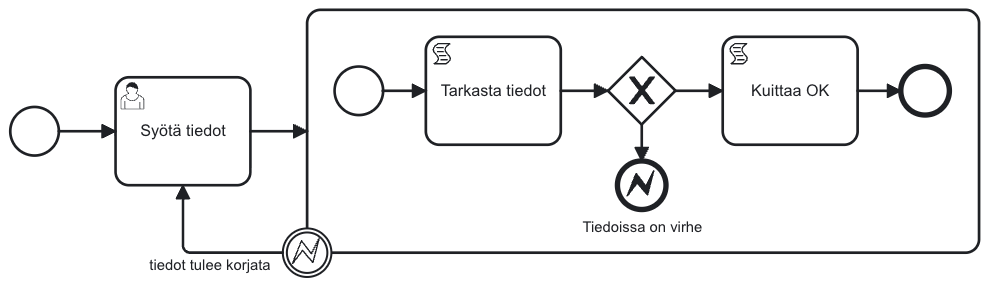
\includegraphics[keepaspectratio]{kuviot/error-esim.png}}

}

\caption{\label{fig-error-esim}Error End Event- ja Error Boundary Event
-tapahtumat}

\end{figure}%

Error End Eventille tulee määritellä virhekoodi ja viite (\emph{Global
error reference}), jonka avulla virheenkäsittely voidaan toteuttaa
(kuva~\ref{fig-error_esim2}). Edellisessä esimerkissä käyttäjää siis
vain pyydettäisiin täyttämään tiedot uudelleen, mutta joissain
tapauksissa voisi olla tarpeen määritellä esimerkiksi korjaava
prosessikulku, joka käynnistettäisiin virheen havaitsemisen jälkeen.

\begin{figure}

\centering{

\pandocbounded{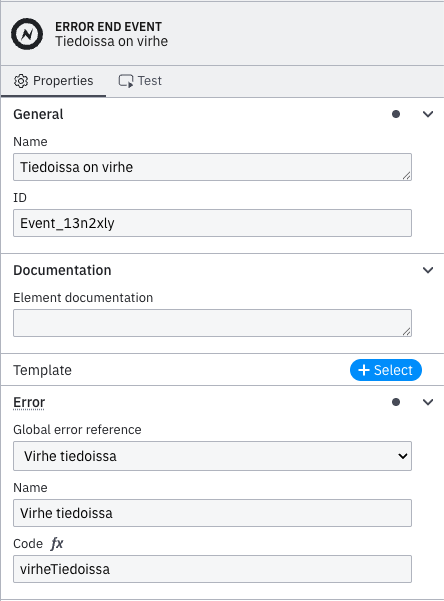
\includegraphics[keepaspectratio]{kuviot/error-esim2.png}}

}

\caption{\label{fig-error_esim2}Virheen määrittely Camundassa}

\end{figure}%

\subsubsection{Compensation Event}\label{compensation-event}

\emph{Compensation Event}iä käytetään kompensoimaan eli kumoamaan jo
suoritettu tehtävä prosessin suorituksen keskeytyessä. Kompensoivan
toimenpiteen suunnittelulla voidaan toteuttaa tehtävän hallittu,
liiketoimintalogiikan mukainen peruuttaminen. Kompensoinnin ei
välttämättä ole tarkoitus palauttaa systeemiä samaan tilaan, jossa se
oli kompensoitavan prosessin tai tehtävän käynnistyessä.

Ajatellaan jotain systeemiä, jolla on useita samanaikaisia käyttäjiä.
Yksi käyttäjistä käynnistää prosessin, jossa prosessimuuttujan
\texttt{luku1} numeroarvosta siirretään puolet muuttujan \texttt{luku2}
arvoon. Jokin tehtävä lukee ensin \texttt{luku1}:n lähtöarvon ja
vähentää siitä puolet. Mikäli \texttt{luku2}:n arvon kasvattaminen
\texttt{luku1}:n puolikkaalla jostain teknisestä tai vaikka
liiketoimintasääntöön perustuvasta syystä kuitenkin epäonnistuu,
transaktiomuotoisessa suorituksessa prosessi keskeytetään (\emph{Abort})
ja systeemi palautetaan sen alkuperäiseen tilaan (\emph{Rollback}). On
kuitenkin mahdollista, että systeemin toinen käyttäjä on tällä välin
päivittänyt \texttt{luku1}:n arvoa, jolloin alkuperäisen tilan
palauttaminen rollback-operaatiolla hävittää myös toisen käyttäjän
tekemän muutoksen. Tarvitaan peräkkäinen palautus (\emph{Cascading
Rollback}), joka peruuttaa kaikki väärän tiedon varassa toteutetut
toiminnot. Yksinkertaisin ratkaisu tietysti olisi lukita kunkin
transaktion tarvitsemat resurssit kyseiselle transaktiolle, kunnes koko
prosessi on suoritettu onnistuneesti loppuun tai keskeytetty.
Liiketoimintaprosessit voivat kuitenkin olla kestoltaan pitkiä, joten
resurssien lukitseminen voisi aiheuttaa huomattavaakin viivettä kaikkiin
muihin samoja resursseja tarvitseviin toimintoihin.

Seuraavassa esimerkissä (kuva~\ref{fig-compensation-esim}) varauspyynnön
vastaanottamisen jälkeen asiakkaalle varataan matkakohteeseen lento ja
hotellimajoitus. Mikäli maksun veloitus ei kuitenkaan onnistu, prosessi
etenee \emph{Compensation End Event} -tapahtumaan ja \emph{Compensation
Boundary Event} -tapahtumat käynnistävät kompensoivat tehtävät.
Kompensoivalle tehtävälle ei ole omaa tehtävätyyppiä, vaan esimerkiksi
Camundassa tehtävään lisätään kompensointia ilmaiseva symboli
automaattisesti, kun tehtävä käynnistyy Compensation Eventin kautta.

\begin{figure}

\centering{

\pandocbounded{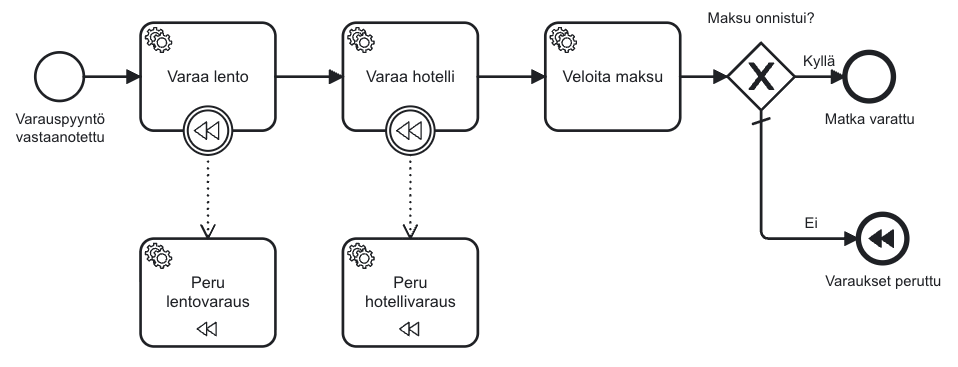
\includegraphics[keepaspectratio]{kuviot/compensation-esim.png}}

}

\caption{\label{fig-compensation-esim}Maksun epäonnistuessa suoritetaan
kompensaatio}

\end{figure}%

Kompensointi koskee vain tehtäviä, jotka on jo tehty loppuun. Jos
prosessi olisi kaatunut jo hotellin varaamiseen, vain lento
peruttaisiin. Peruminen -- tai kumoaminen -- ei ole tekninen rollback,
vaan sitä varten täytyy määritellä oma toimenpiteensä, eikä
kompensoinnin tarvitse siis palauttaa systeemiä täsmälleen alkutilaan.
Esimerkiksi lennon peruutuksesta voisi asiakkaalle jäädä maksettavaksi
peruutusmaksu.

\subsubsection{Link Event}\label{link-event}

\emph{Link Event}in avulla voidaan yhdistää prosessin osia ilman
fyysistä virtayhteyttä. Sitä voidaan verrata joistain
ohjelmointikielistä tuttuun goto-käskyyn, joka siirtää ohjelman
suorittamisen toiseen kohtaan ohjelmakoodia. Link Eventin toteuttama
siirto on yksisuuntainen eli sen jälkeen suorittamista ei palauteta
takaisin, toisin kuin vaikka funktiota ohjelmointikielessä kutsuttaessa.

Link Eventiä käytetään lähinnä monimutkaisten prosessimallien
selkeyttämiseen sen mahdollistaessa prosessimallin pilkkomisen
pienempiin osiin ja hypyt osien välillä.

Seuraavassa prosessissa (kuva~\ref{fig-link-esim}) puuttuvan tuotteen
tilaamisen jälkeen Link Event \emph{Toimitukseen} siirtää prosessikulun
\emph{Toimita tilaus} -aliprosessin käynnistämiseen.

\begin{figure}

\centering{

\pandocbounded{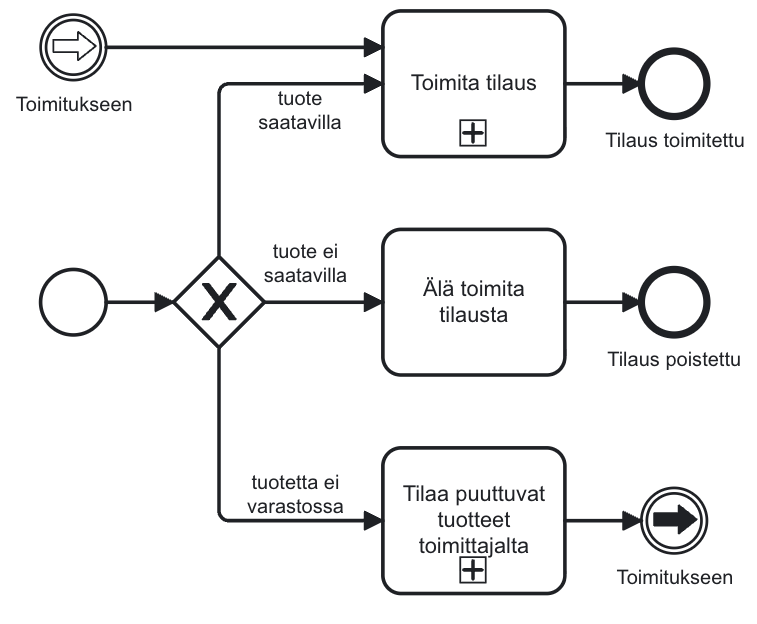
\includegraphics[keepaspectratio]{kuviot/link-esim.png}}

}

\caption{\label{fig-link-esim}Link Event}

\end{figure}%

\subsubsection{Signal Event}\label{signal-event}

Siinä missä Message-tehtävät ja -tapahtumat on aina tarkoitettu tarkoin
koordinoituun kahden osapuolen väliseen viestinvaihtoon, \emph{Signal
Event} mahdollistaa samanaikaisen \emph{broadcast}-tyyppisen viestinnän
useille signaalia kuunteleville. Signaalin lähettäjän ei tarvitse
tietää, kuinka monta vastaanottajaa sillä on, eikä se odota
vastaanottajilta vastausta (kuva~\ref{fig-signal-token-esim}).

Signal Event -tapahtuman tyypit ovat heittävä (\emph{Throw}) ja
vastaanottava (\emph{Catch}). Sitä voidaan käyttää \emph{Boundary}-,
\emph{Intermediate}-, \emph{Start}- ja \emph{End}-tapahtumissa.

Seuraavassa esimerkissä tehtävää \emph{1} seuraa Intermediate Signal
Event \emph{A}. Kaksi muuta prosessia kuuntelevat tätä signaalia ja sen
saatuaan suorittavat omat tehtävänsä \emph{2} ja \emph{3}. Signaloiva
prosessi siis pyytää kaikkia signaalin \emph{A} kuulevia prosesseja
Signal Start Eventin kautta suorittamaan omat tehtävänsä ja siirtyy
suorittamaan tehtäväänsä \emph{4}.

Teknisesti ottaen -- ja automaattisia prosessikulkuja simuloitaessa --
tehtävien \emph{2} ja \emph{3} suorittaminen alkaa samaan aikaan kuin
tehtävän \emph{4}. Mikäli tehtävillä ei ole määriteltyä suoritusaikaa,
ne kaikki myös valmistuvat samaan aikaan. Käytännössä ja todellisissa
prosesseissa tätä ei tietenkään voida taata.

\begin{figure}

\centering{

\pandocbounded{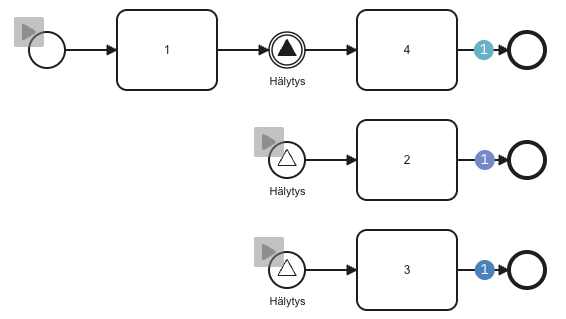
\includegraphics[keepaspectratio]{kuviot/signal-token-esim.png}}

}

\caption{\label{fig-signal-token-esim}Signal Eventin suorittaminen
prosessisimulaatiossa\sidenote{\footnotesize Kuviossa näkyvä Token Simulation
  esitellään Työvälineitä-luvussa.}}

\end{figure}%

Käytäntöä lähempänä olevassa esimerkissä laadunvarmistus huomaa ongelman
jossain myytävässä tuotteessa ja prosessi signaloi siitä
(kuva~\ref{fig-signal-ongelma}).

\begin{figure}

\centering{

\pandocbounded{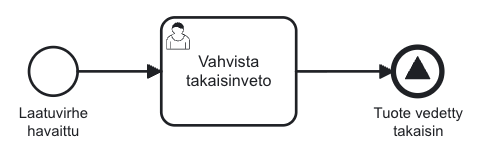
\includegraphics[keepaspectratio]{kuviot/signal-ongelma.png}}

}

\caption{\label{fig-signal-ongelma}Myytävässä tuotteessa on havaittu
ongelma}

\end{figure}%

Kaikki tilausten keräilyprosessit, jotka saavat tiedon kerättävään
tilaukseen kuuluvan tuotteen takaisinvedosta, keskeytetään.

\begin{figure}

\centering{

\pandocbounded{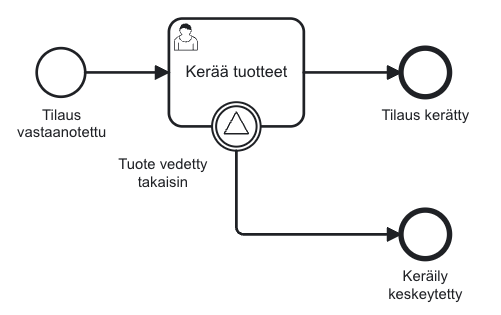
\includegraphics[keepaspectratio]{kuviot/signal-reaktio.png}}

}

\caption{\label{fig-signal-reaktio}Keräily keskeytetään tilatun tuotteen
ongelman vuoksi}

\end{figure}%

\subsubsection{None Event}\label{none-event}

\emph{None Event} on tyhjä tapahtuma, jossa ei varsinaisesti
prosessikulun kannalta tapahdu mitään (kuva~\ref{fig-none-esim}). Niitä
voidaan käyttää prosessin luettavuuden parantamiseen ohjelmakoodin
kommentoinnin tavoin tai pitkäkestoisen prosessin tilasiirtymien
konkreettiseen tarkastamiseen.

None Eventit pystyvät myös asettamaan muuttujia, joten niitä voidaan
hyödyntää prosessin monitoroinnissa (esimerkiksi KPI-mittareihin
liittyvä informaatio) tai automatisoitujen prosessien toteutuksessa
tarvittavien ohjausyksityiskohtien asettamisessa.

\begin{figure}

\centering{

\pandocbounded{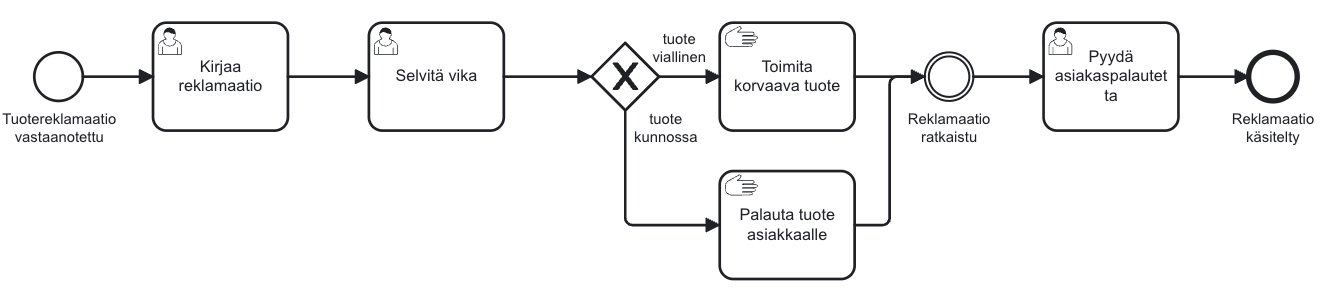
\includegraphics[keepaspectratio]{kuviot/reklamaation-kasittely.png}}

}

\caption{\label{fig-none-esim}Reklamaatio ratkaistu -None Event}

\end{figure}%

Vaikka None Event ei varsinaisesti tee mitään, se voi kertoa prosessista
ja sen tilasta paljonkin. Sen avulla (\emph{Reklamaatio ratkaistu})
edellinen prosessi jaettiin kahteen konkreettiseen vaiheeseen: ongelman
selvittämiseen ja reklamaation käsittelyn jälkitoimiin. Yrityksen
palvelulupaus voi olla, että reklamaatio ratkaistaan viidessä
arkipäivässä. Tässä voidaan prosessin kokonaiskeston sijaan mitata aikaa
aloituksesta välitavoitteeseen, koska korvaavan tuotteen toimituksen
kesto ei ole reklamaatioiden käsittelijöiden hallinnassa. Lisäksi
asiakaspalvelija näkee käynnissä olevasta prosessi-instanssista, onko
reklamaatio jo ratkaistu, vaikka prosessi ei olisi vielä päättynyt.

\subsection{Portit}\label{portit}

Porttien (\emph{Gateway}) avulla voidaan ohjata prosessin etenemistä
tietyissä päätöspisteissä prosessin aikana. Portit voivat myös
haarauttaa (\emph{Split}) prosessivirran useaan suuntaan ja yhdistää
(\emph{Join}) useita virtoja taas yhdeksi. Portin symbolina käytetään
vinoneliötä, jonka sisällä on portin tyyppiä ilmaiseva tunnus.

\subsubsection{Parallel Gateway}\label{parallel-gateway}

\emph{Parallel Gateway} eli rinnakkainen portti jakaa prosessivirran
useaan rinnakkain suoritettavaan haaraan. Rinnakkaisen portin
tunnisteena käytetään +-merkkiä. Rinnakkaiset virrat tulisi taas
yhdistää, kun se on mahdollista.

Seuraavassa esimerkissä (kuva~\ref{fig-til-toimi}) prosessin kulku
haarautuu kolmeen rinnakkaiseen järjestysvirtaan, jotka aktivoituvat
samanaikaisesti.

\begin{figure}

\centering{

\pandocbounded{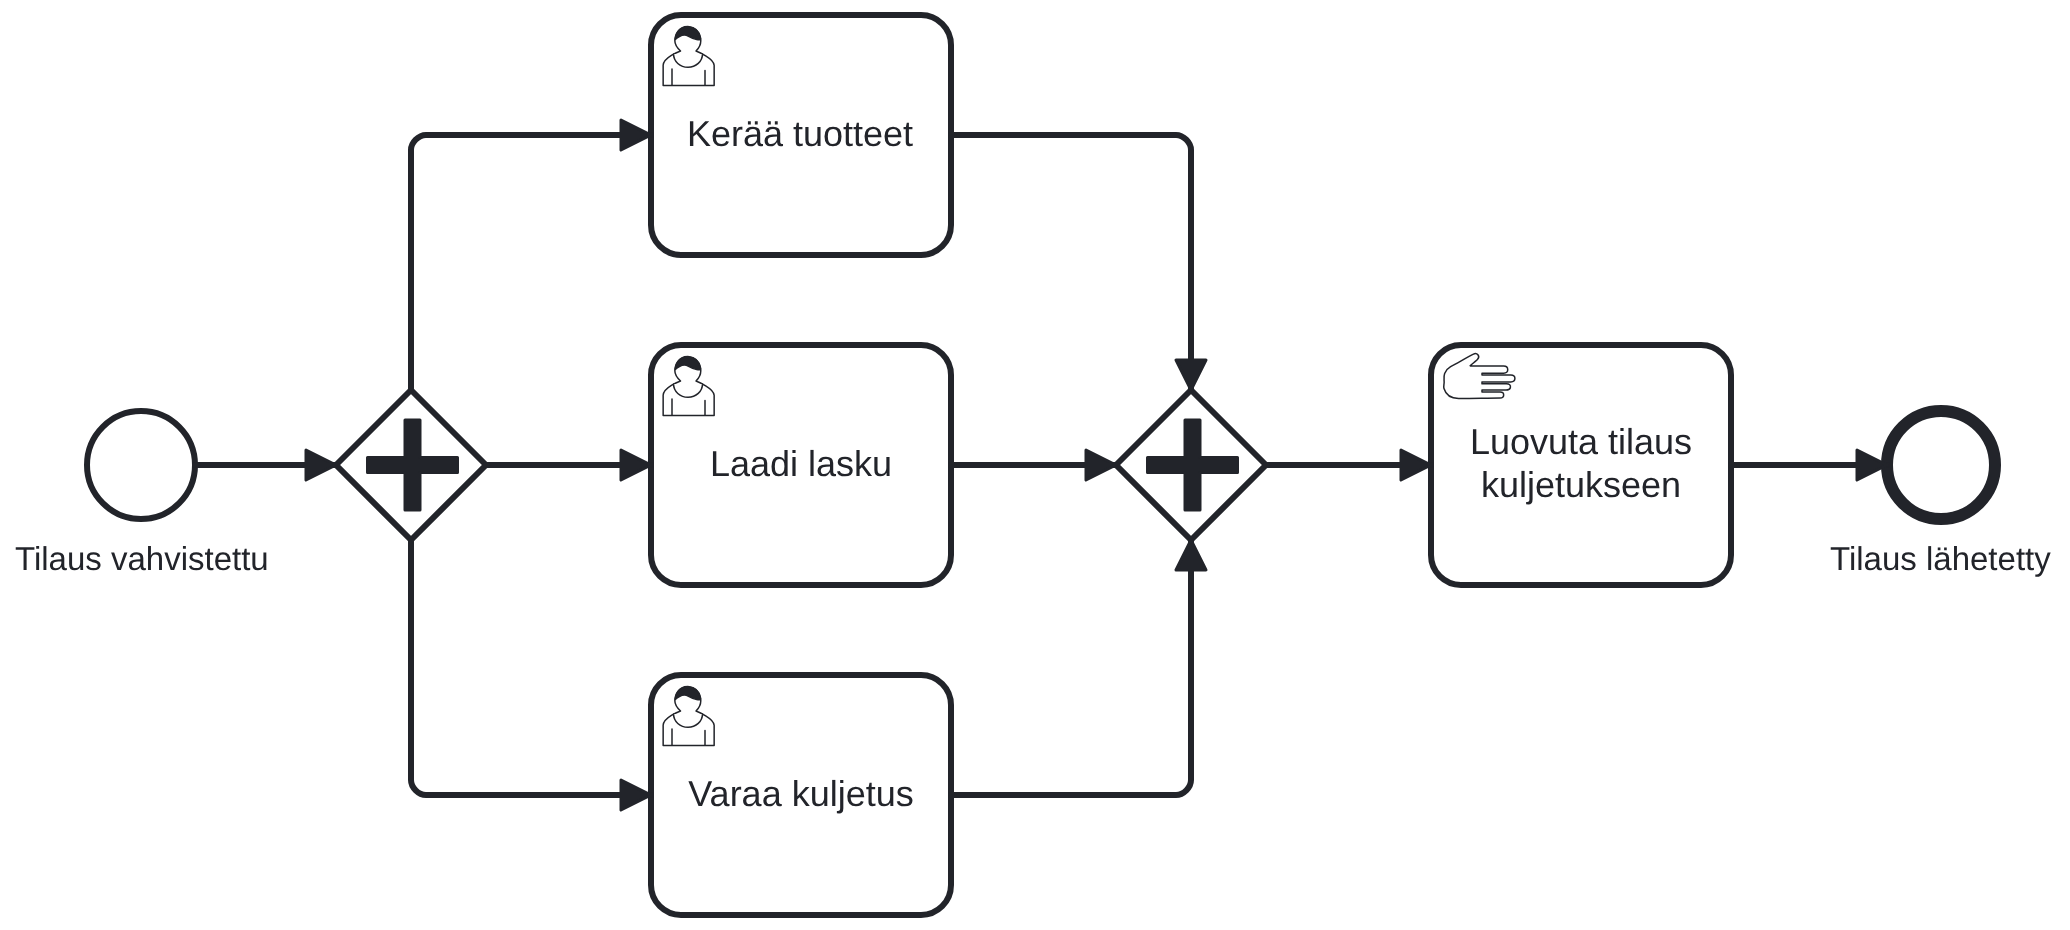
\includegraphics[keepaspectratio]{kuviot/tilauksen-toimitus.png}}

}

\caption{\label{fig-til-toimi}Tilaus toimitukseen kolmella rinnakkain
suoritettavalla tehtävällä}

\end{figure}%

\subsubsection{Exclusive Gateway}\label{exclusive-gateway}

\emph{Exclusive Gateway} eli eksklusiivinen portti tai XOR-portti
merkitään vinoneliön sisällä olevalla ✕-merkillä. Sen avulla prosessin
kulkua voidaan ohjata sääntöperusteisesti: XOR-portti valitsee ehtojen
perusteella vain yhden etenemispolun.

Mikäli useampi XOR-porttiin liittyvä ehto on tosi, prosessi seuraa
ensimmäistä tosi-haaraa. Tällaisia tilanteita on syytä pyrkiä
välttämään. Ehtojen tulisi siis olla toisensa poissulkevia. Tarvittaessa
voidaan tukeutua myös oletusvirran merkitsemiseen.

Seuraavassa esimerkissä (kuva~\ref{fig-xor-esim}) eksklusiivinen portti
jatkuu kolmeen vaihtoehtoiseen järjestysvirtaan. Mikäli asiakas on uusi,
hänelle lähetetään tervetuliaisviesti. Mikäli asiakkuus on kestänyt
vuoden, lähetetään kiitokset pitkästä asiakassuhteesta. Muissa
tapauksissa viestejä ei lähetellä. Ilman viestin lähettämistä etenevä
järjestysvirta on merkitty oletusvirraksi.

\begin{figure}

\centering{

\pandocbounded{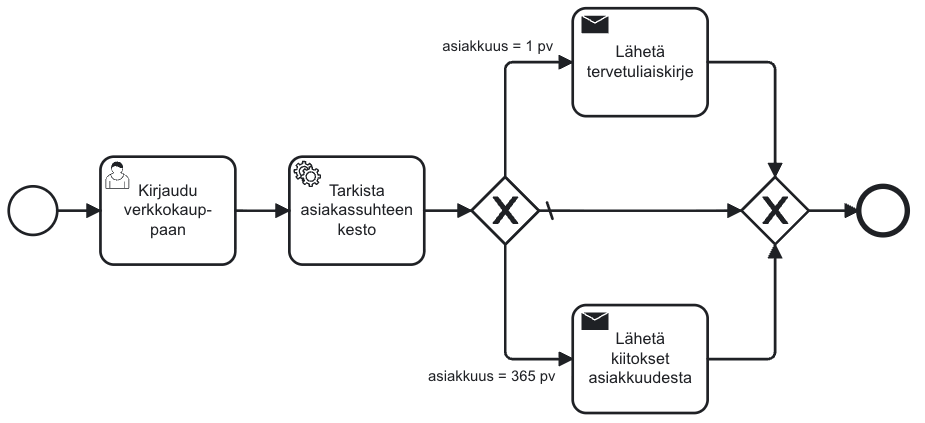
\includegraphics[keepaspectratio]{kuviot/xor-esim1.png}}

}

\caption{\label{fig-xor-esim}Kolmehaarainen XOR-portti}

\end{figure}%

Ehdot (\emph{Condition}) määritellään portista lähteviin virtoihin
(kuva~\ref{fig-xor-esim2}) ja prosessia suoritettaessa se etenee
prosessimuuttujien arvojen mukaisesti (kuva~\ref{fig-xor-esim3}).

\begin{figure}

\centering{

\pandocbounded{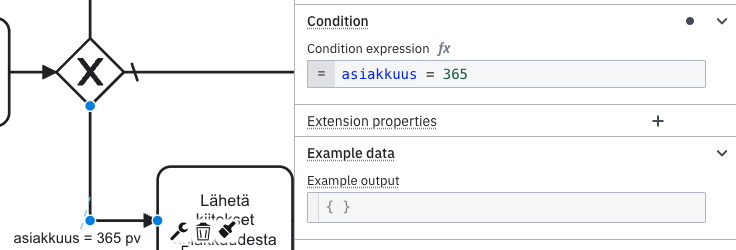
\includegraphics[keepaspectratio]{kuviot/xor-esim2.png}}

}

\caption{\label{fig-xor-esim2}XOR-portista lähteville haaroille tulee
määritellä yksiselitteiset ja toisensa poissulkevat ehdot}

\end{figure}%

\begin{figure}

\centering{

\pandocbounded{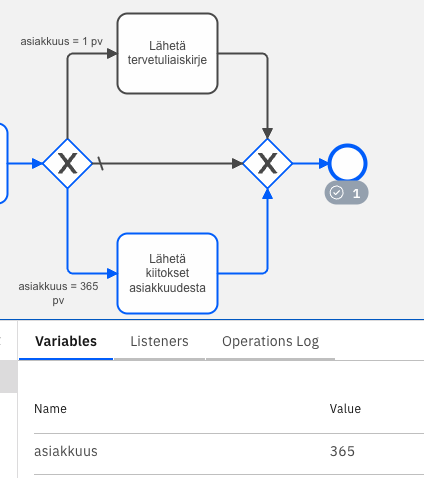
\includegraphics[keepaspectratio]{kuviot/xor-esim3.png}}

}

\caption{\label{fig-xor-esim3}Prosessia suoritettaessa verrataan
virtojen ehtoja muuttujien arvoihin}

\end{figure}%

Ehdot kannattaa kirjoittaa myös virtojen yhteyteen, jotta prosessimallin
lukeminen graafisen esityksen perusteella on helpompaa.

\subsubsection{Inclusive Gateway}\label{inclusive-gateway}

\emph{Inclusive Gateway} eli inklusiivinen portti tai yleisemmin
OR-portti merkitään vinoneliön sisällä olevalla ympyrällä. Porttia
seuraavista virroista valitaan ehtojen perusteella yksi tai useampia.
OR-portti voi siis aktivoida useita haaroja ja vähintään yhden haaran
täytyy aina aktivoitua.

Seuraavassa esimerkissä (kuva~\ref{fig-inclu-esim}) VIP-asiakkaille
annetaan viiden prosentin alennus ja yli kymmenen tilausta tehneille
asiakkaille 2,5 prosentin alennus. Molempien ehtojen täyttyessä asiakas
voi siis saada molemmat alennukset.

\begin{figure}

\centering{

\pandocbounded{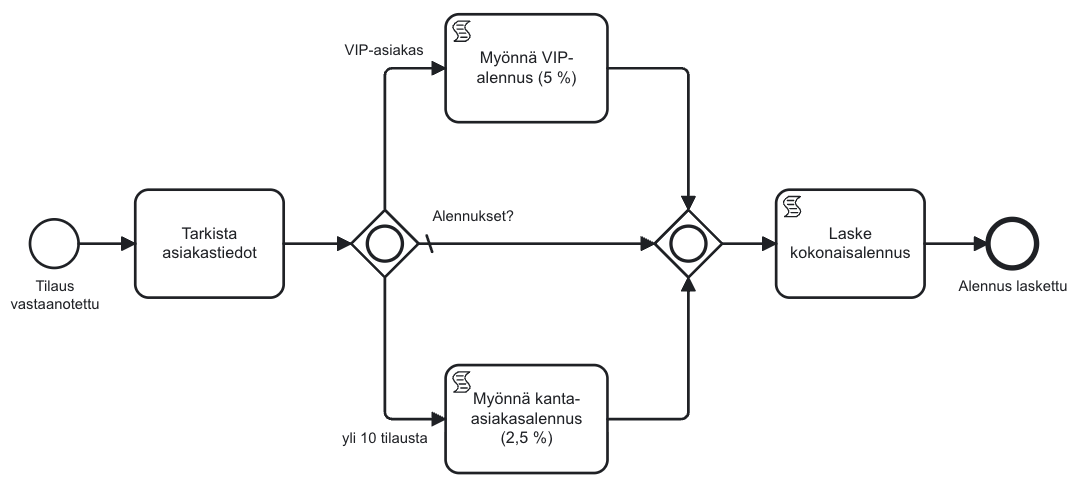
\includegraphics[keepaspectratio]{kuviot/inclu-esim.png}}

}

\caption{\label{fig-inclu-esim}Alennusten aktivointi OR-portilla}

\end{figure}%

OR-portin haarojen ehdot tarkastetaan ja haarat aktivoituvat
tarvittaessa. Ylemmässä haarassa tarkastetaan \texttt{vip}-muuttujan
arvo ja mikäli se on \texttt{true} (kuva~\ref{fig-inclu-esim2}),
asetetaan skriptitehtävällä muuttujan \texttt{vipAlennus} arvoksi
\texttt{5} (kuva~\ref{fig-inclu-esim3}).

\begin{figure}

\centering{

\pandocbounded{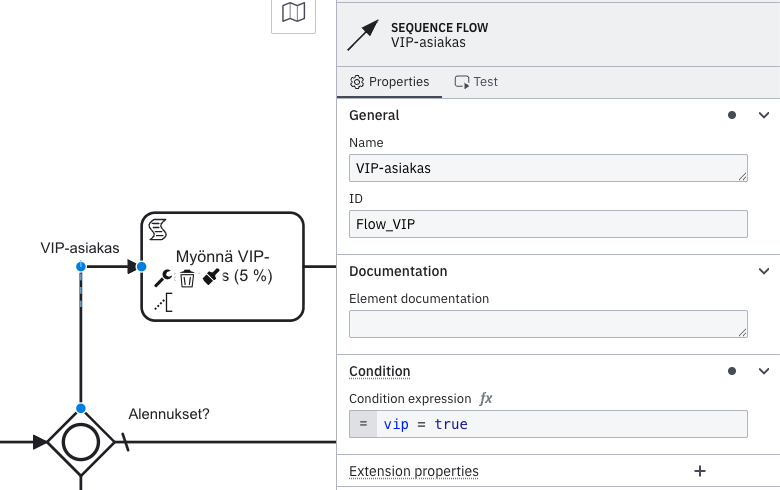
\includegraphics[keepaspectratio]{kuviot/inclu-esim2.png}}

}

\caption{\label{fig-inclu-esim2}Tunnistetaan VIP-asiakas}

\end{figure}%

\begin{figure}

\centering{

\pandocbounded{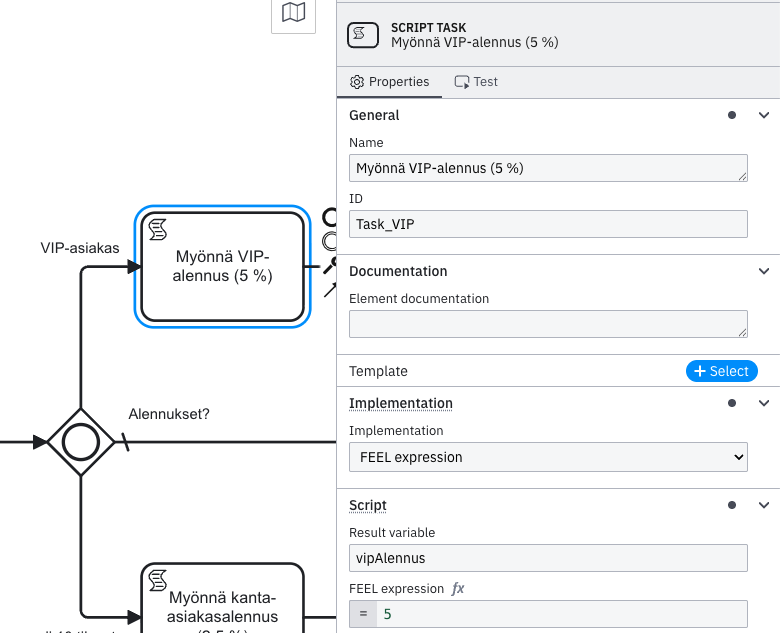
\includegraphics[keepaspectratio]{kuviot/inclu-esim3.png}}

}

\caption{\label{fig-inclu-esim3}Asetetaan VIP-alennus}

\end{figure}%

Myös alempi haara tarkastetaan ja tarvittaessa asetetaan muuttujalle
\texttt{kantaAlennus} arvo \texttt{2.5}. Lopuksi \emph{Laske
kokonaisalennus} -tehtävässä kokonaisalennus muodostetaan
FEEL-skriptillä (kuva~\ref{fig-inclu-esim4}). Mikäli
\texttt{vipAlennus}- ja \texttt{kantaAlennus}-muuttujia ei ole asetettu,
saavat ne arvon \texttt{0}.

\begin{figure}

\centering{

\pandocbounded{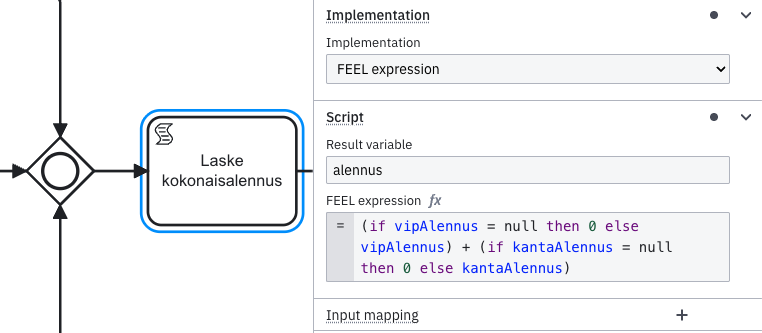
\includegraphics[keepaspectratio]{kuviot/inclu-esim4.png}}

}

\caption{\label{fig-inclu-esim4}Lasketaan kokonaisalennus}

\end{figure}%

\subsubsection{Event-Based Gateway}\label{event-based-gateway}

\emph{Event-Based Gateway} eli tapahtumapohjainen portti suorittaa
valinnan sen perusteella, mikä siihen liittyvistä tapahtumista tapahtuu
ensimmäisenä\sidenote{\footnotesize On mahdollista, että useampi Event-Based Gatewayn
  odottama tapahtuma tapahtuisi täsmälleen samaan aikaan.
  Automatisoidussa prosessissa näin ei kuitenkaan voi käydä.
  Reaaliaikaiset ja rinnakkaislaskentaa toteuttavat järjestelmätkin
  käsittelevät samaan kokonaisuuteen tai prosessiin liittyvät tehtävät
  aina jonkinlaisessa peräkkäisjärjestyksessä, vaikka niiden käsittely
  tapahtuisikin nanosekunneissa. Viimeistään prosessia suorittava
  prosessimoottori voisi ratkaista tilanteen valitsemalla jonkin
  samanaikaisista tehtävistä suoritettavaksi ensimmäisenä järjestelmän
  sisäisen aikaleiman tai prioriteettilogiikan mukaan.}. Prosessin kulku
siis aina odottaa vähintään hetken ensimmäistä tapahtumaa. Sen sijaan
esimerkiksi joko-tai-muotoinen XOR-portti päästää virran läpi
välittömästi, koska päätökseen tarvittavat tiedot menevät porttiin
syötteinä. Event-Based Gateway merkitään vinoneliön sisällä olevalla
kaksiviivaisella ympyrällä, jonka sisällä on viisikulmio.

Koska Event-Based Gateway odottaa seuraavaa tapahtumaa, voivat prosessin
suorituksessa sitä seurata erilaiset tapahtumatyyppiset elementit eli
\emph{Conditional Catch Event}, \emph{Message Catch Event}, \emph{Signal
Catch Event} ja \emph{Timer Event}. Näiden lisäksi voidaan sallia myös
viestin vastaanottava tehtävä \emph{Receive Task}.

Seuraavassa esimerkissä (kuva~\ref{fig-event-based-esim}) käytetään
tapahtumapohjaista porttia prosessissa, jossa Service Task kutsuu jotain
ulkoista palvelua API-rajapinnan kautta. Tapahtumapohjaiseen porttiin
mentäessä ei vielä tiedetä, saadaanko palvelulta vastaus. Porttia seuraa
kaksi vaihtoehtoista tapahtumaa: viestin vastaanottava tapahtuma, joka
nappaa ulkoisen palvelun vastauksen sen saapuessa sekä Timer, joka
palauttaa prosessin palvelukutsuun kymmenen sekunnin kuluttua. Mikäli
kutsuttu palvelu ei siis vastaa kymmenen sekunnin sisällä, Timer
aktivoituu ensin ja palvelua kutsutaan uudelleen. Jos taas vastaus
saapuu ennen tätä, prosessi jatkaa eteenpäin.

\begin{figure}

\centering{

\pandocbounded{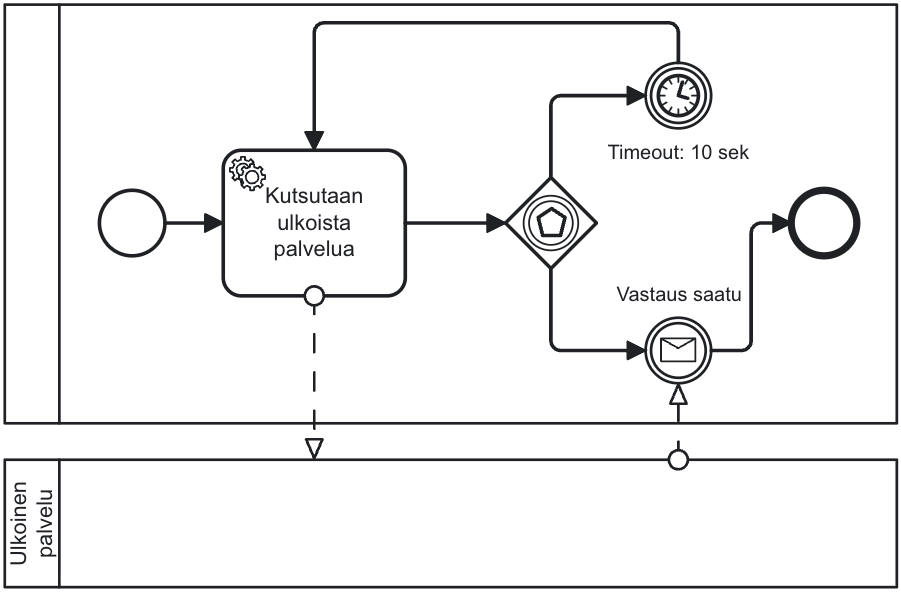
\includegraphics[keepaspectratio]{kuviot/event-based-esim.png}}

}

\caption{\label{fig-event-based-esim}Event-Based Gateway ulkoista
palvelua kutsuttaessa}

\end{figure}%

\subsubsection{Complex Gateway}\label{complex-gateway}

\emph{Complex Gateway} eli kompleksiportti soveltuu monimutkaisten ja
moniosaisten ehtojen määrittelyyn. Sitä käytetään prosessimalleissa
kuitenkin harvoin ja usein sama logiikka on esitettävissä myös muiden
porttien avulla -- joskin voi olla, että prosessimallista tulee tällöin
monimutkaisempi. Mainittakoon anekdoottina, että prosessiarkkitehti ja
-analyytikko Allen Murrell on sanonut, että niiden 15 vuoden aikana, kun
hän on prosesseja mallintanut, hän on luultavasti käyttänyt
kompleksiporttia kahdesti ja silloinkin varmaan olisi onnistunut
rakentamaan mallin myös toisella tavalla\sidenote{\footnotesize ''I think in the
  fifteen years that I've been modeling processes I've possibly used the
  Complex Gateway twice and even then I've probably could have modeled
  it in a different way using other gateway, even just one or two more
  gateways.''}.

Seuraavassa esimerkissä (kuva~\ref{fig-complex-esim}) esitetään
eräänlaisen tarjouspyyntöprosessin kulku. Complex Gateway -portin
tehtävänä tässä on päästää prosessi etenemään silloin kun kaksi kolmesta
materiaalinmyyjästä on toimittanut tarjouksen.

\begin{figure}

\centering{

\pandocbounded{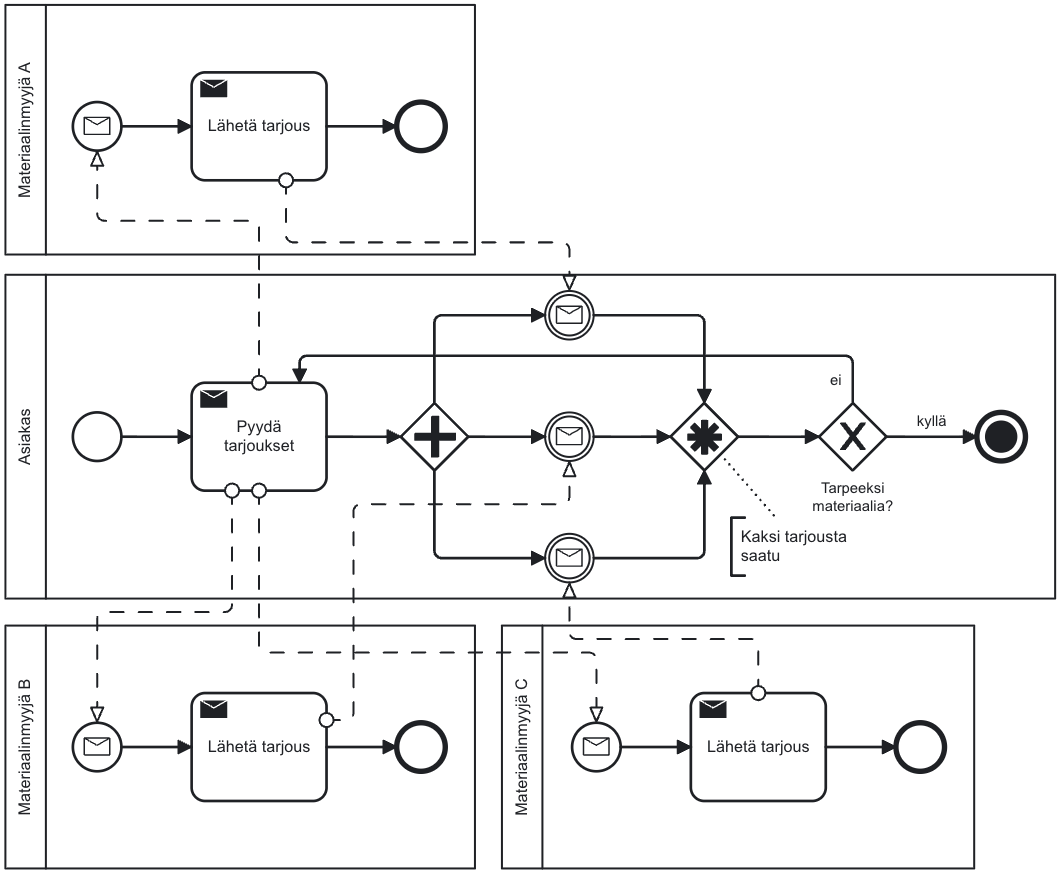
\includegraphics[keepaspectratio]{kuviot/complex-esim.png}}

}

\caption{\label{fig-complex-esim}Complex Gateway -portti
tarjouspyyntöprosessissa}

\end{figure}%

\subsection{Tietolähteet ja ohjelmistot
BPMN-prosessimalleissa}\label{tietoluxe4hteet-ja-ohjelmistot-bpmn-prosessimalleissa}

Prosesseja mallinnettaessa ollaan ensisijaisesti kiinnostuneita
prosessien toimintalogiikasta eikä niinkään prosesseihin liittyvistä
ohjelmistoista tai tietolähteistä. Haluttaessa tarkastella prosessia
vaikkapa suhteessa niihin liiketoiminta- ja teknologiaympäristöihin,
joissa se tapahtuu, ovat esimerkiksi arkkitehtuurimallinnukset sopivampi
työväline. Jotkin mallinnusvälineet mahdollistavat myös useiden
mallinnuskielten samanaikaisen käyttämisen. Tällöin prosesseja voidaan
esimerkiksi kokonaisarkkitehtuurin kontekstissa tarkastella
ArchiMate-kaavioina ja tarvittaessa siirtyä jonkin prosessikulun
tarkempaan tarkasteluun BPMN-muodossa (kuva~\ref{fig-porautuminen}).

\begin{figure}

\centering{

\pandocbounded{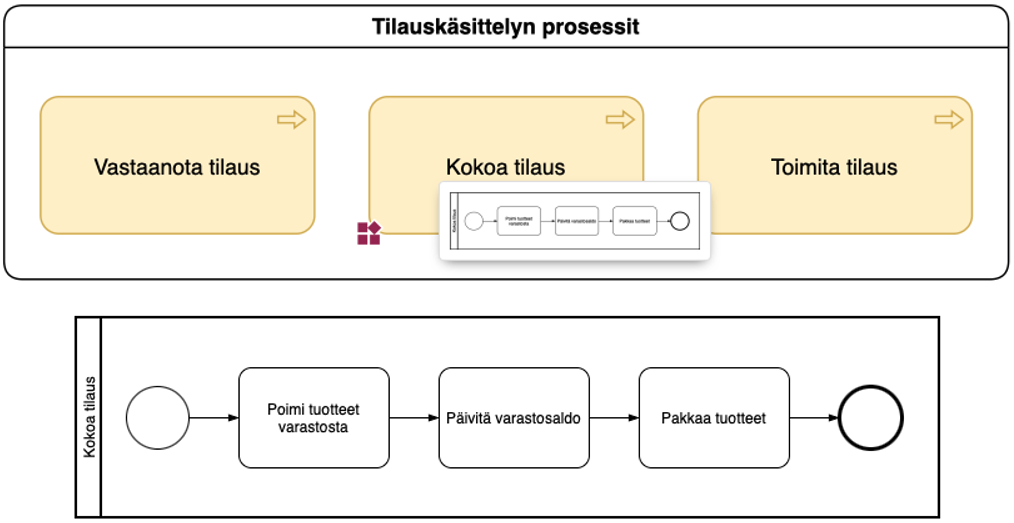
\includegraphics[keepaspectratio]{kuviot/porautuminen.png}}

}

\caption{\label{fig-porautuminen}Porautuminen ArchiMate-notaatiolla
esitetyn prosessin kautta tarkempaan BPMN-muotoiseen esitykseen Arter
ARC -työvälineessä}

\end{figure}%

Järjestelmillä ja niiden rajapinnoilla, tietokoneiden suorittamilla
skripteillä sekä prosesseissa liikkuvalla informaatiolla ja datalla on
kuitenkin keskeinen rooli varsinkin silloin, kun prosesseja halutaan
automatisoida. Edellä onkin jo käsitelty Service Task -tehtäviä, joita
käytetään ulkoisten palvelujen (eli käytännössä ohjelmistojen ja
tietojärjestelmien) kutsumiseen, Script Task -tehtäviä, joiden avulla
voidaan suorittaa ohjelmakoodia prosessikulun sisällä sekä User Task
-tehtäviä, jotka nekin tyypillisesti toteutetaan jotain ohjelmistoa
hyödyntäen.

Luvun alussa nähtiin myös Data Store -elementti ja siihen liittyvät Data
Input Association ja Data Output Association -suhteet. Data Storea
voidaan käyttää tietovarastojen, tietokantojen tai muiden
''tietosäiliöiden'' esittämiseen prosessikulkujen yhteydessä. Joskus
niitä käytetään myös yleisemminkin kuvaamaan prosessissa käytettäviä
tietojärjestelmiä ja ohjelmistoja, ja niille voidaan varata prosessiin
oma uimarata tai -allas. Vaikka tämä onkin hieman luovaa BPMN:n
soveltamista, on tekniikka melko usein käytetty ja joissain --
pääasiassa viestinnällisissä -- käyttötarkoituksissa myös
käyttökelpoinen (kuva~\ref{fig-datastoret}).

\begin{figure}

\centering{

\pandocbounded{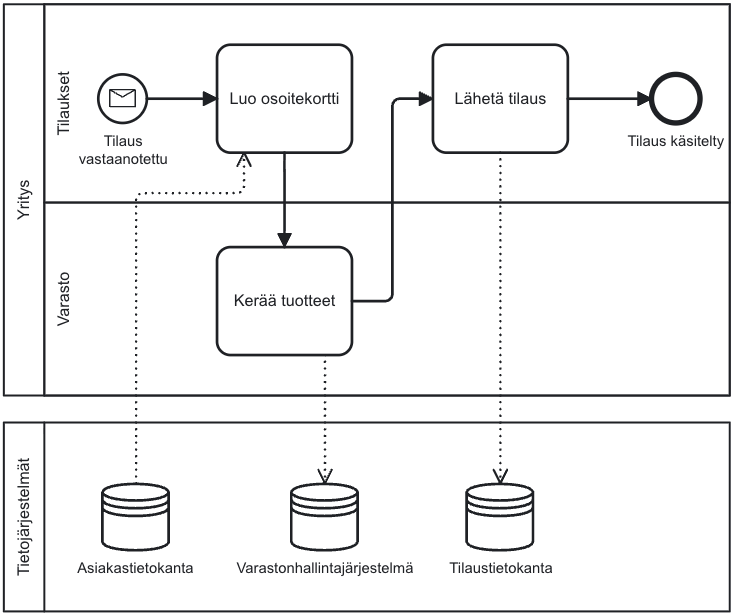
\includegraphics[keepaspectratio]{kuviot/datastoret.png}}

}

\caption{\label{fig-datastoret}Prosessin käyttämien tietokantojen ja
järjestelmien esittäminen Data Store -elementtien avulla}

\end{figure}%

Ohjelmallista toimintalogiikkaa voidaan joissain tapauksissa myös
jäsentää prosessin tehtävien avulla (kuva~\ref{fig-riski}). Mitä enemmän
automatisoidussa prosessissa käytetään skriptitehtäviä, skriptattuja
päätössääntöjä ja päätöstauluja, sitä enemmän ero prosessin ja
varsinaisen sovelluksen välillä hämärtyy. Prosessikehittäjistä tulee
ohjelmistokehittäjiä tai ohjelmistokehittäjistä prosessikehittäjiä.

\begin{figure}

\centering{

\pandocbounded{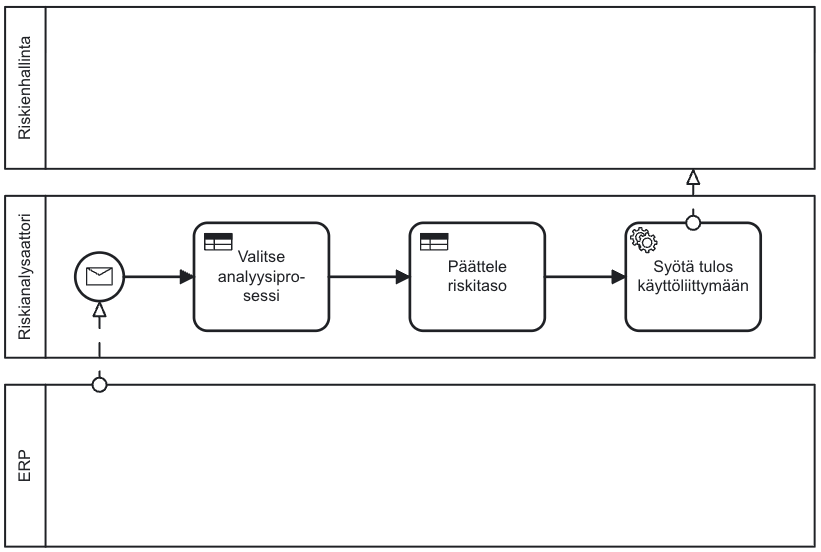
\includegraphics[keepaspectratio]{kuviot/riski-esim.png}}

}

\caption{\label{fig-riski}Riskianalysaattorin toimintalogiikkaa}

\end{figure}%

\subsection[Julkinen ja yksityinen prosessi: kollaboraatio, orkestraatio
ja koreografia]{\texorpdfstring{Julkinen ja yksityinen prosessi:
kollaboraatio, orkestraatio ja
koreografia\sidenote{\footnotesize Käsitteet esitetään tässä BPMN 2.0 -standardin
  mukaisesti (ks. standardin luku 7.2,
  https://www.omg.org/spec/BPMN/2.0.2/PDF). Esimerkiksi palvelukeskeisen
  arkkitehtuurin ja mikropalveluarkkitehtuurin yhteydessä
  orkestraatiolla ja koreografialla tarkoitetaan hieman eri asioita, ja
  myös mallinnusvälineet voivat käyttää termejä omilla tavoillaan.}}{Julkinen ja yksityinen prosessi: kollaboraatio, orkestraatio ja koreografia}}\label{julkinen-ja-yksityinen-prosessi-kollaboraatio-orkestraatio-ja-koreografiakoreo-kasitteet}

Prosessien yhteistyötä mallinnettaessa esiin nousevat käsitteet
yksityinen prosessi (\emph{Private Process}) ja julkinen prosessi
(\emph{Public Process}).

Yksityinen prosessi on organisaation sisäinen prosessi, jossa esitetään
kaikki sen tehtävät, portit ja tapahtumat. Yksityinen prosessi voi olla
myös suoritettava (\emph{executable}) eli työnkulkualustalla ajettavaksi
tarkoitettu. Kuvassa (kuva~\ref{fig-yksityinen}) on verkkokaupan
tilausprosessi yksityisenä prosessina. Asiakas on kuvattu suljettuna
altaana (\emph{black box}), koska verkkokauppa ei tiedä -- eikä sen
tarvitsekaan tietää -- millainen asiakkaan kunkin prosessi on.

\begin{figure}

\centering{

\pandocbounded{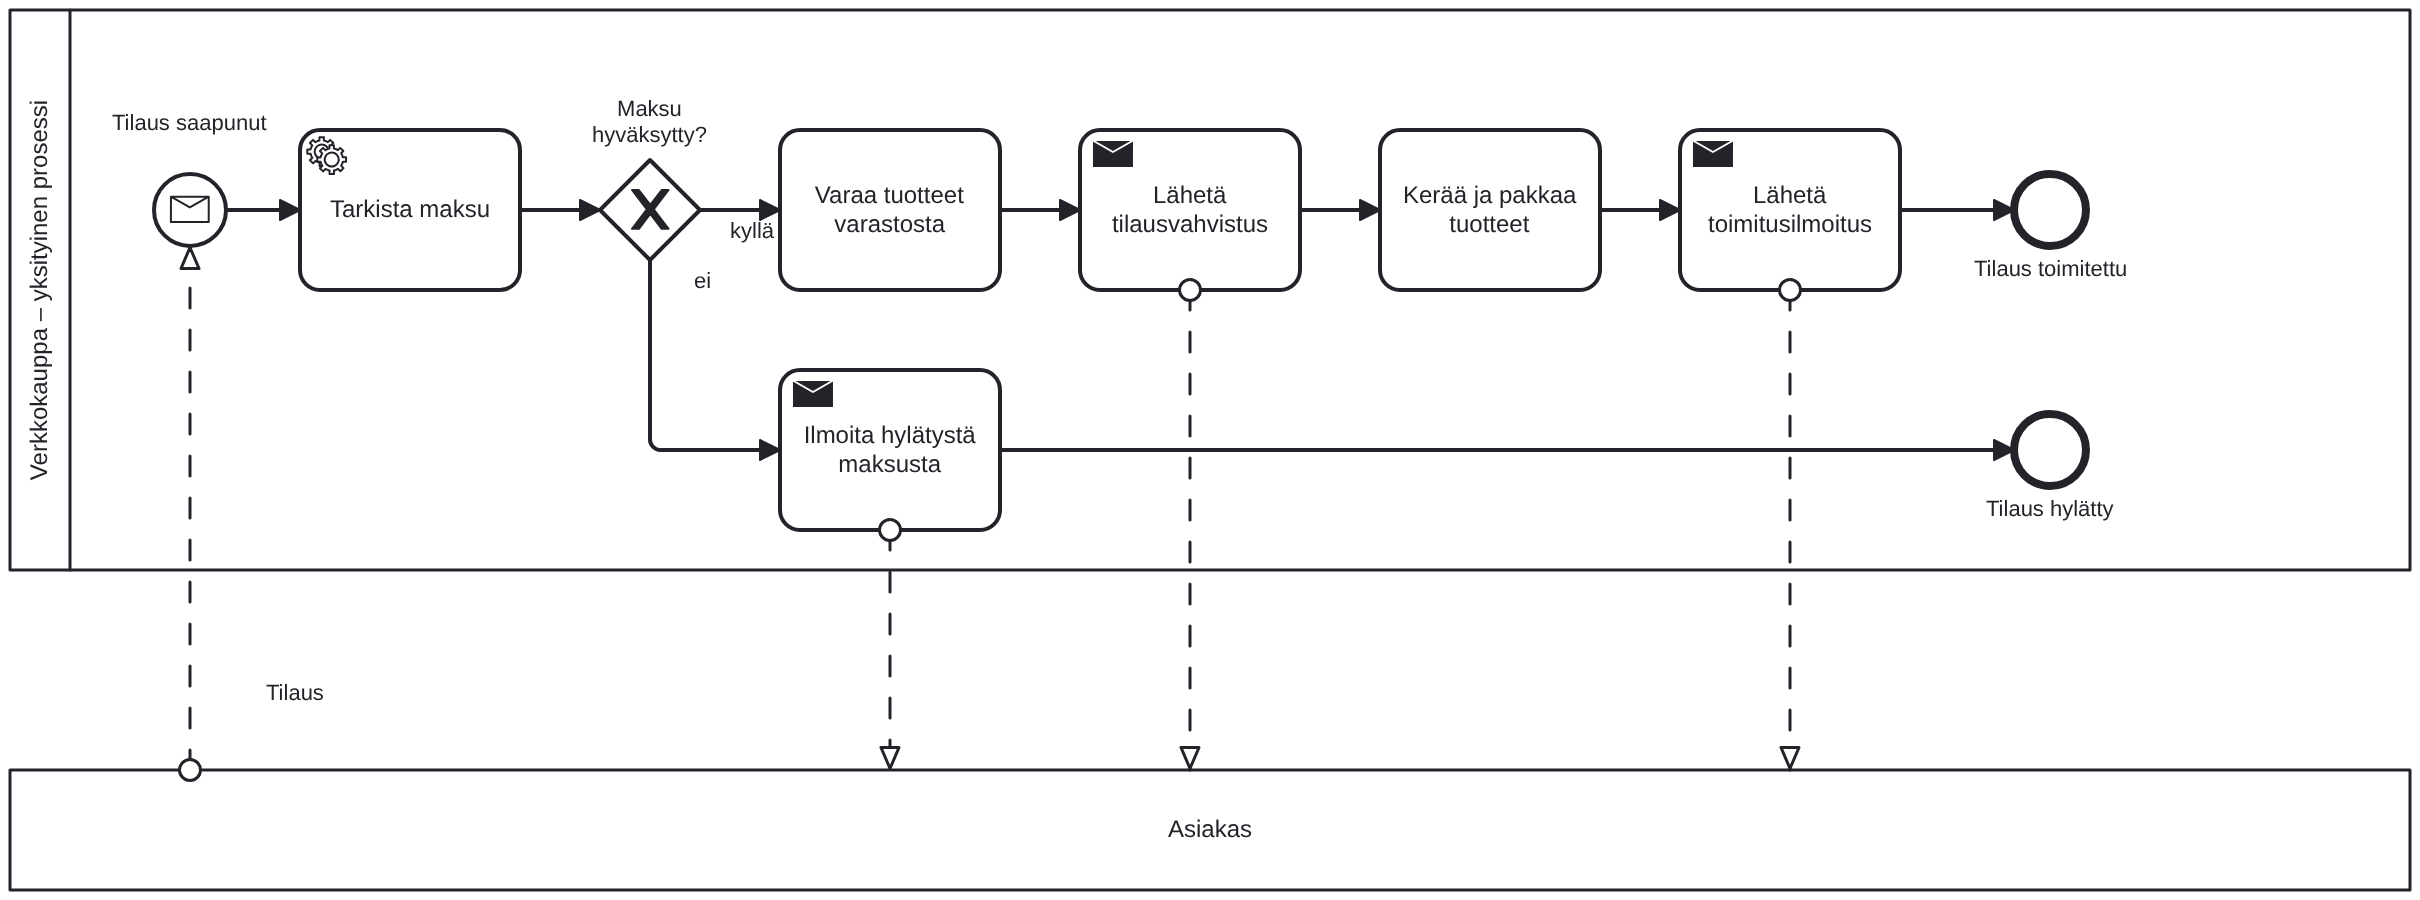
\includegraphics[keepaspectratio]{kuviot/yksityinen-prosessi.png}}

}

\caption{\label{fig-yksityinen}Verkkokaupan tilausprosessi yksityisenä
prosessina}

\end{figure}%

Julkinen prosessi näyttää samasta prosessista vain ne osat, joiden
kautta osapuoli on vuorovaikutuksessa muiden kanssa. Tämä tarkoittaa
viestejä lähettäviä ja vastaanottavia tehtäviä, tapahtumia sekä kulkua
niiden välillä. Sisäiset tehtävät, kuten maksun tarkistus, tuotteiden
varaaminen ja keräily, jäävät pois (kuva~\ref{fig-julkinen}). Julkinen
prosessi on siis tavallaan prosessin ulospäin näkyvä rajapinta.

\begin{figure}

\centering{

\pandocbounded{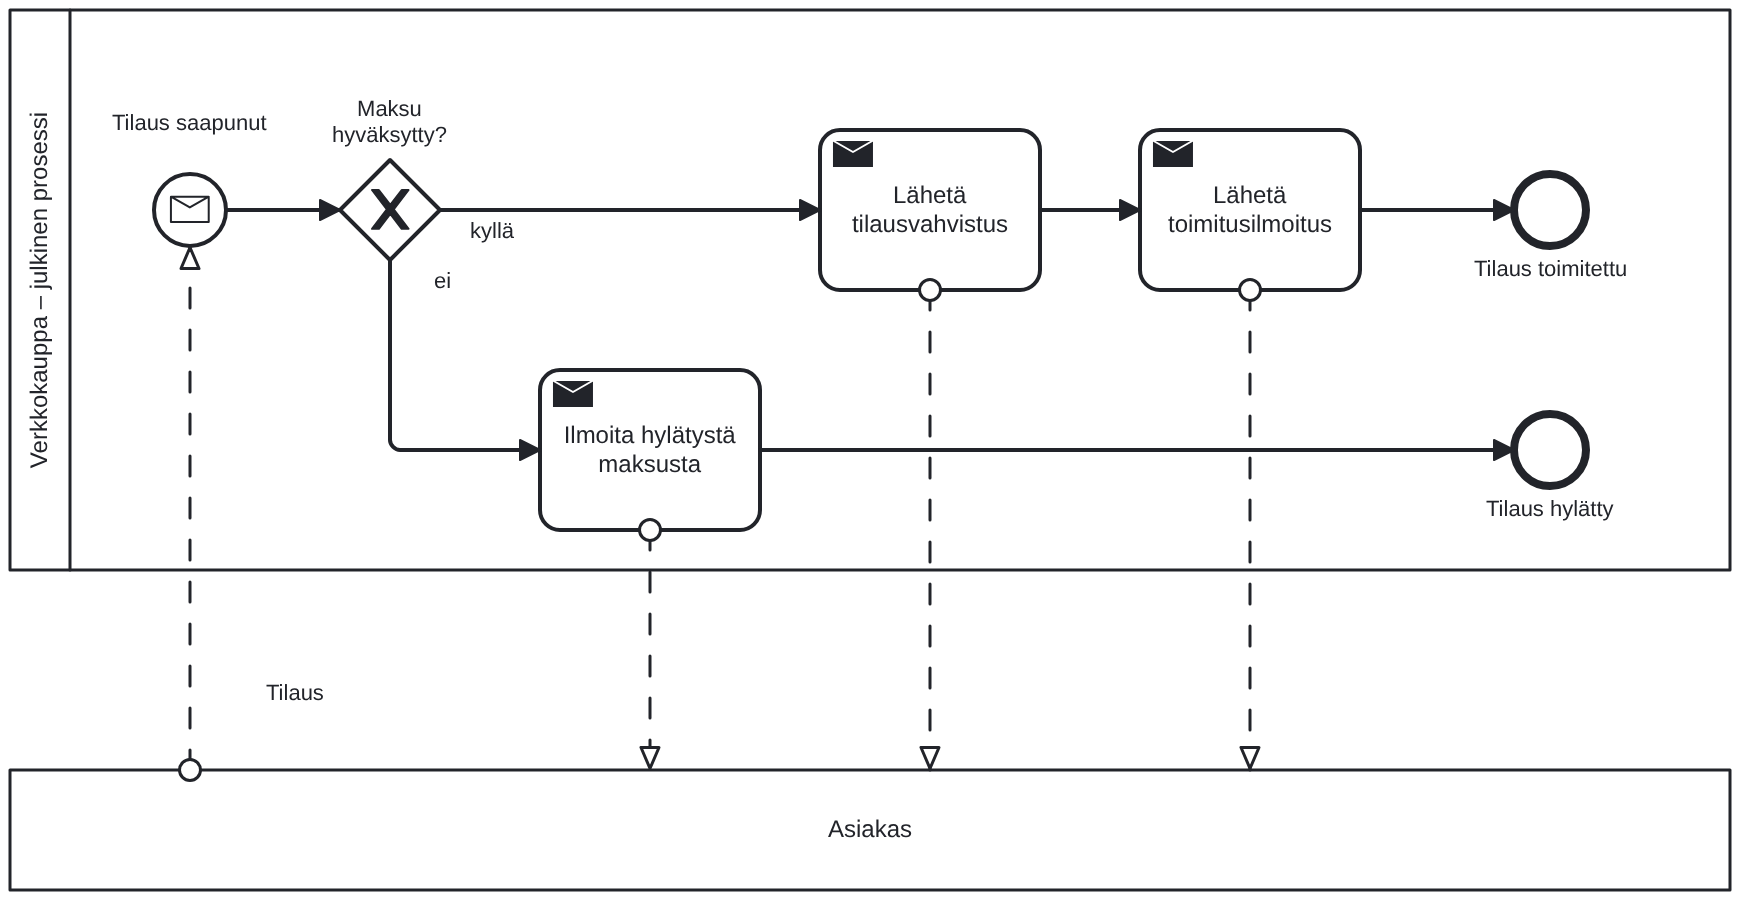
\includegraphics[keepaspectratio]{kuviot/julkinen-prosessi.png}}

}

\caption{\label{fig-julkinen}Saman tilausprosessin julkinen prosessi}

\end{figure}%

Liiketoimintaverkoston osapuolten ei tarvitse tuntea toistensa sisäisiä
prosesseja, kunhan ne tietävät, mitä viestejä ne voivat toisiltaan
odottaa ja missä järjestyksessä viestit liikkuvat. Yksityiset prosessit
voivat siis piilottaa prosessin sisäisen toimintalogiikan ja olla siten
kirjaimellisestikin yksityisiä.

Yhteistyöprosesseihin liittyvät myös käsitteet kollaboraatio
(\emph{Collaboration}), orkestraatio (\emph{Orchestration}) ja
koreografia (\emph{Choreography}). Ne kuvaavat eri näkökulmista sitä,
miten osallistujat, esimerkiksi organisaatiot, osastot tai sovellukset,
toimivat yhdessä prosessin aikana.

\subsubsection{Kollaboraatio}\label{kollaboraatio}

Kollaboraatiomalli kuvaa kaksi tai useampia prosessiin osallistuvia
osapuolia sekä näiden välisen vuorovaikutuksen. BPMN:ssä osapuolet
esitetään uima-altaina ja vuorovaikutus viestivirtoina. Altaat voivat
olla avattuja, jolloin niissä näkyy osapuolen yksityinen tai julkinen
prosessi, tai suljettuja, jolloin osapuolesta näkyvät vain sen
lähettämät ja vastaanottamat viestit. Edellisetkin kuvat
(kuva~\ref{fig-yksityinen} ja kuva~\ref{fig-julkinen}) ovat siis
kollaboraatiomalleja. Itse asiassa kaikki aiemmat esimerkit, joissa on
useampi allas ja niitä yhdistäviä viestivirtoja, ovat
prosessikollaboraatioita.

Kollaboraatiomallissa kaikki altaat voidaan esittää myös suljettuina
(kuva~\ref{fig-verkkokauppa-kollab}). Silloin malli kertoo ainoastaan,
mitä viestejä osapuolten välillä kulkee. Esitystapa muistuttaa hieman
UML:n sekvenssikaaviota, mutta toisin kuin sekvenssikaaviossa, viestien
järjestys ei ole yksiselitteinen, koska se riippuu altaiden sisällä
olevista prosesseista.

\begin{figure}

\centering{

\pandocbounded{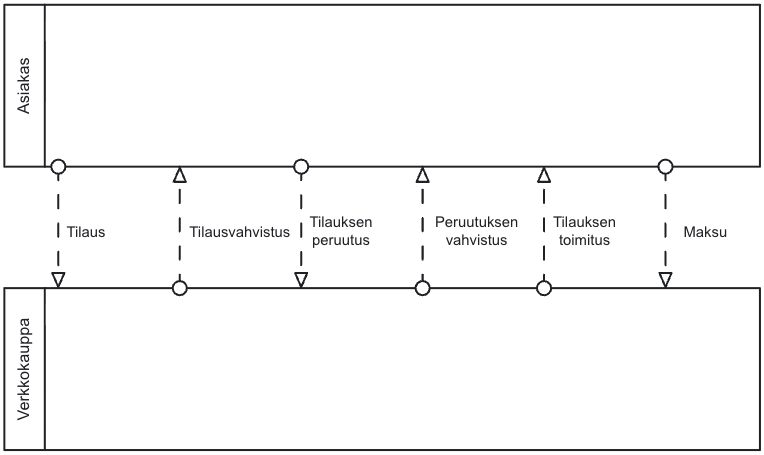
\includegraphics[keepaspectratio]{kuviot/verkkokauppa-kollab.png}}

}

\caption{\label{fig-verkkokauppa-kollab}Verkkokaupan ja asiakkaan
vuorovaikutusta ilmaiseva kollaboraatiomalli, jossa molemmat altaat on
suljettu}

\end{figure}%

\subsubsection{Orkestraatio}\label{orkestraatio}

Orkestraatio kuvaa yhden osapuolen ohjaamaa yhteistyötä.
Orkesterinjohtajan tavoin tämä toimija koordinoi prosessin etenemistä.
Se kutsuu muita osapuolia, odottaa niiden vastauksia ja päättää
vastausten perusteella, mitä seuraavaksi tapahtuu. Muut osapuolet eivät
tunne kokonaisuutta, vaan ne ainoastaan vastaavat niille osoitettuihin
pyyntöihin.

BPMN:ssä orkestraatio on yksityinen prosessi, joka on mallinnettu auki
tehtävien ja tapahtumien tarkkuudella. Muut osallistujat kuvataan
suljettuina altaina, joihin kulkee viestivirtoja. Tyypillisesti
orkestroiva prosessi on suoritettava, ja sitä ajetaan
työnkulkualustalla, joka kutsuu muiden osapuolten järjestelmiä niiden
rajapintojen kautta. Seuraavassa kuvassa (kuva~\ref{fig-orkestraatio})
verkkokaupan tilausprosessi ohjaa maksupalvelua, varastoa ja
kuljetusliikettä sekä tiedottaa asiakkaalle tilauksen etenemisestä.

\begin{figure}

\centering{

\pandocbounded{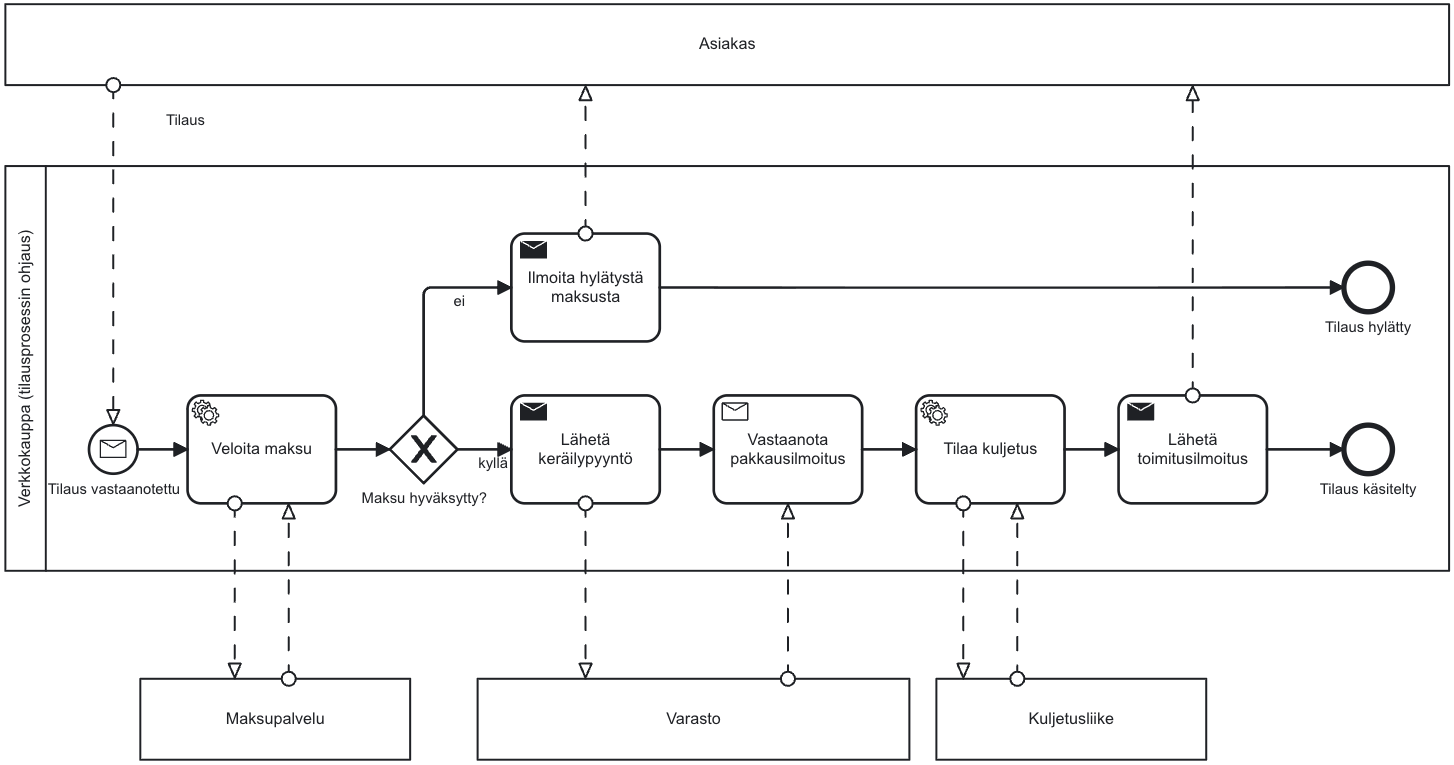
\includegraphics[keepaspectratio]{kuviot/orkestraatio-verkkokauppa.png}}

}

\caption{\label{fig-orkestraatio}Verkkokaupan tilausprosessi orkestroi
maksupalvelua, varastoa ja kuljetusliikettä}

\end{figure}%

Orkestraatiossa kokonaisuuden hallinta on yhdellä osapuolella. Tämä
tekee prosessin seurannasta ja muuttamisesta suoraviivaista, mutta
samalla orkestroiva prosessi on toimintokokonaisuuden kriittinen piste.
Jos ei pysähtyy, eivät myöskään orkestroidut prosessit etene.

\subsubsection{Koreografia}\label{koreografia}

Prosessikoreografiassa millään osapuolella ei ole prosessikulkua
ohjaavaa roolia, eikä prosessilla siten myöskään keskitettyä ohjausta.
Koreografia on kaikkien osallistujien yhteistoimintaa, jolle on
määritelty ennalta sovitut vuorovaikutussäännöt, joita noudattaen
jokainen osallistuja toimii itsenäisesti. Jos prosessiorkestraatio
vertautuu orkesteriin ja sitä johtavaan kapellimestariin, voidaan
prosessikoreografiaa verrata tanssiteokseen. Kun tanssijat tuntevat
koreografian, kukin tietää, mitä hänen tulee tehdä ja milloin, kuinka
asemoida itsensä suhteessa muihin tanssijoihin ja niin edelleen. Teoksen
esittäminen ei edellytä, että koreografi seisoisi tanssijoiden edessä ja
ohjaisi suoritusta, koska se on suunniteltu ja harjoiteltu valmiiksi.
Vastaavasti prosessikoreografia vaatii huolellista suunnittelua ja
osapuolten yhteistyötä, jotta yhteistyöprosessi saadaan toteutettua
luotettavasti pelkästään ennalta sovittuun viestinvaihtoon tukeutuen.

BPMN:ssä koreografialla on oma kaaviotyyppinsä, joka poikkeaa prosessi-
ja kollaboraatiomalleista. Koreografiakaaviossa ei ole uima-altaita,
eikä siinä näy yhdenkään osapuolen sisäinen prosessi. Sen sijaan kaavion
perusyksikkö on koreografiatehtävä (\emph{Choreography Task}), joka
kuvaa yhtä osapuolten välistä viestinvaihtoa. Koreografiatehtävän ylä-
ja alareunassa on osallistujanauhat (\emph{Participant Band}), joihin on
merkitty viestinvaihdon osapuolet. Vaalealla pohjalla oleva nauha on
viestinvaihdon aloittaja (\emph{initiating participant}) ja harmaa nauha
vastaanottaja. Nauhaan liitetty kirjekuori kertoo, mikä viesti
vaihdetaan. Valkoinen kirjekuori on aloittajan lähettämä viesti ja
harmaa kirjekuori vastaanottajan paluuviesti. Koreografiatehtäviä
yhdistetään järjestysvirroilla ja porteilla samaan tapaan kuin
tavallisia tehtäviä, ja koreografialla on aloitus- ja lopetustapahtuma.

Kuvassa (kuva~\ref{fig-koreografia}) on verkkokaupan tilaus
koreografiana. Asiakas aloittaa koreografian lähettämällä tilauksen,
johon verkkokauppa vastaa kuittauksella. Jos tuotteet ovat saatavilla,
verkkokauppa toimittaa tilauksen, ja asiakas maksaa sen. Muussa
tapauksessa verkkokauppa peruu tilauksen ja ilmoittaa siitä asiakkaalle.

\begin{figure}

\centering{

\pandocbounded{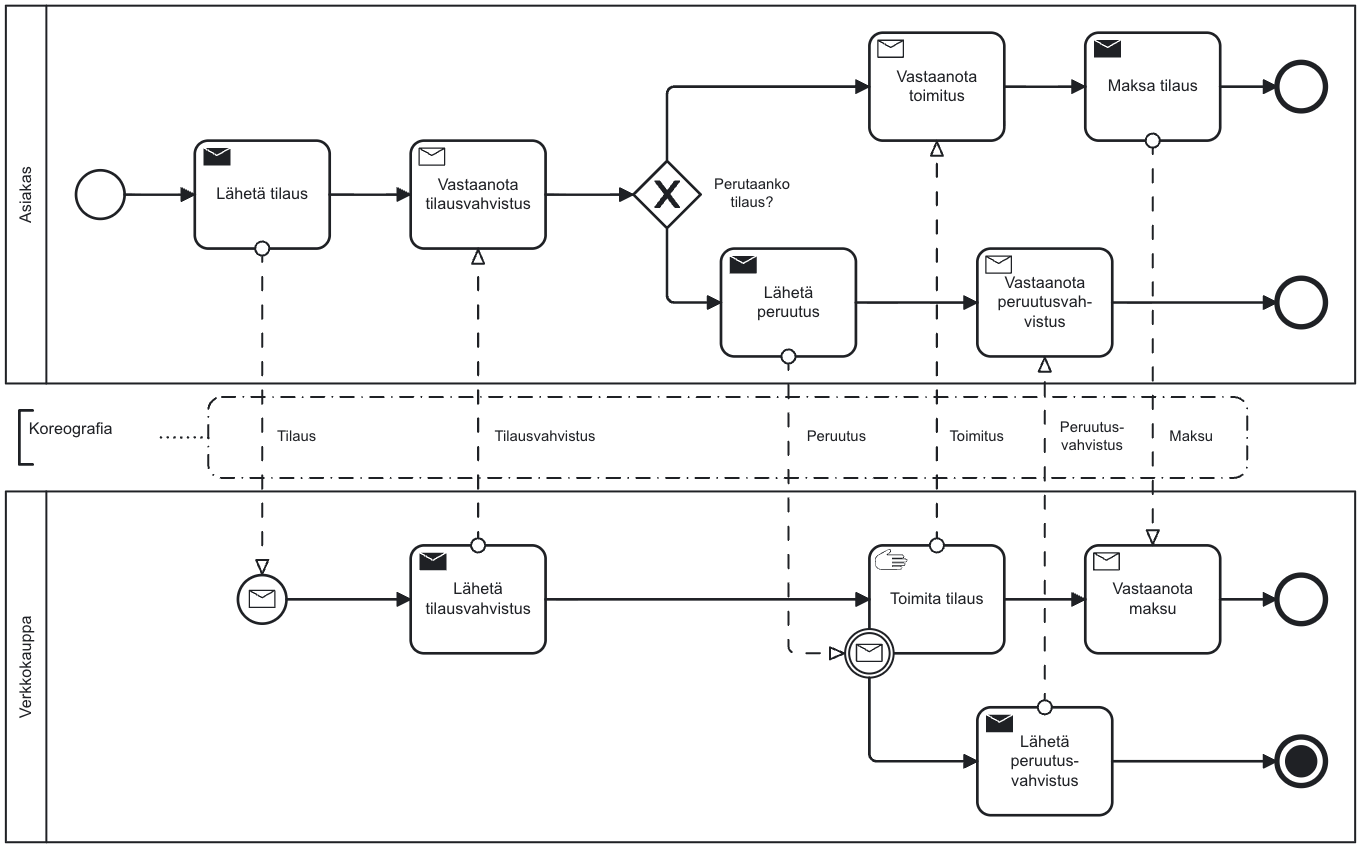
\includegraphics[keepaspectratio]{kuviot/koreografia-verkkokauppa.png}}

}

\caption{\label{fig-koreografia}Verkkokauppatilauksen koreografia}

\end{figure}%

Koska koreografiassa ei ole ohjaavaa osapuolta, mallin on oltava
sellainen, että jokainen osapuoli pystyy toimimaan oikein pelkästään
saamiensa viestien perusteella. BPMN-standardi asettaa tästä syystä
koreografioille sääntöjä. Esimerkiksi koreografiatehtävän aloittajan on
täytynyt osallistua edelliseen viestinvaihtoon, jotta se tietää, että on
sen vuoro toimia. Samoin portin jälkeisten viestinvaihtojen aloittajien
on täytynyt nähdä tieto, jolla porttia seuraava polku valitaan.
Esimerkissä verkkokauppa aloittaa sekä toimituksen että peruutuksen, ja
valinta perustuu sen omaan tietoon tuotteiden saatavuudesta.

Säännöt paljastavat helposti yhteistyön suunnitteluvirheitä. Jos
esimerkiksi asiakkaan sallittaisiin perua tilaus milloin tahansa ennen
toimitusta (kuten kollaboraatiomallissa
kuva~\ref{fig-verkkokauppa-kollab}), sekä asiakas että verkkokauppa
voisivat aloittaa oman viestinvaihtonsa samanaikaisesti: asiakas
lähettää peruutuksen, kun verkkokauppa on jo lähettänyt tilauksen
matkaan. Koreografiaa mallintaessa tällaiset tilanteet tulevat näkyviin,
ja osapuolten on sovittava, kumman ratkaisu on voimassa; esimerkiksi
niin, että peruutus on mahdollinen vain siihen asti, kun verkkokauppa on
ilmoittanut lähettävänsä tilauksen.

Mallinnusvälineet tukevat koreografiakaavioita heikommin kuin prosessi-
ja kollaboraatiomalleja. Esimerkiksi Camunda Modeler ei tue niitä.
Koreografiakaavioita voi kuitenkin laatia esimerkiksi avoimen
lähdekoodin chor-js-välineellä\sidenote{\footnotesize https://github.com/bptlab/chor-js}.
Käytännössä yritysten välistä yhteistyötä kuvataankin usein
kollaboraatiomalleilla, ja koreografioita käytetään erityisesti silloin,
kun usean organisaation on sovittava yhteisestä viestinvaihdosta, eikä
kenenkään sisäinen prosessi ole varsinaisesti kiinnostuksen kohteena.

\section{Joitain muita tapoja prosessien
kuvaamiseen}\label{joitain-muita-tapoja-prosessien-kuvaamiseen}

Prosessien kuvaamiseen voidaan käyttää muitakin tekniikoita kuin
BPMN-kieltä. Tässä luvussa käydään niistä läpi muutama.

\subsection{Prosessikortti}\label{prosessikortti}

Prosessikortti on teksti- tai graafinen dokumentti, joka kokoaa
prosessiin liittyvät oleelliset tiedot. Kortti voi käyttötarkoituksensa
mukaisesti käsitellä prosessia yleisellä tasolla tai vastaavasti kortin
sisältö voi olla yksityiskohtaistakin. Korttia voidaan hyödyntää niin
prosessitiedon keräämisessä kuin myös prosessitiedon tallentamisessa ja
esittämisessä. Kortti voi toimia itsenäisenä prosessidokumentaation
välineenä tai se voidaan laatia graafisen prosessimallin liitteeksi.
Prosessikorttia voidaan käyttää esimerkiksi prosessihaastattelun
dokumentointiin. Se voitaisiin harkinnanvaraisesti myös toimittaa
haastateltavalle henkilölle ennakkomateriaaliksi ennen haastattelua.

Seuraavassa (Taulukko~\ref{tbl-prosessikortti-esim}) on verkkokaupan
kuvitteellisesta tilauskäsittelyprosessista laadittu tiivis
prosessikortti.

\begin{longtable}[]{@{}
  >{\raggedright\arraybackslash}p{(\linewidth - 2\tabcolsep) * \real{0.4667}}
  >{\raggedright\arraybackslash}p{(\linewidth - 2\tabcolsep) * \real{0.5333}}@{}}
\caption{Esimerkki prosessikortista: verkkokaupan
tilauskäsittely}\label{tbl-prosessikortti-esim}\tabularnewline
\toprule\noalign{}
\begin{minipage}[b]{\linewidth}\raggedright
Kohta
\end{minipage} & \begin{minipage}[b]{\linewidth}\raggedright
Kuvaus
\end{minipage} \\
\midrule\noalign{}
\endfirsthead
\toprule\noalign{}
\begin{minipage}[b]{\linewidth}\raggedright
Kohta
\end{minipage} & \begin{minipage}[b]{\linewidth}\raggedright
Kuvaus
\end{minipage} \\
\midrule\noalign{}
\endhead
\bottomrule\noalign{}
\endlastfoot
\textbf{Prosessin nimi} & Verkkokaupan tilauskäsittely \\
\textbf{Tavoite} & Varmistaa tilauksen oikea ja ajantasainen käsittely
ja toimitus sekä asiakastyytyväisyys. \\
\textbf{Prosessin alku} & Asiakas tekee tilauksen verkkokaupassa. \\
\textbf{Prosessin loppu} & Tilaus on toimitettu asiakkaalle ja tilaus
suljettu järjestelmässä. \\
\textbf{Keskeiset vaiheet} & 1. Tilauksen vastaanotto järjestelmään.2.
Maksun varmistus.3. Tuotteiden keräys ja pakkaus.4. Toimituksen
organisointi.5. Lähetyksen seuranta ja viestintä asiakkaalle. \\
\textbf{Prosessin omistaja} & Verkkokaupan tilausvastaava. \\
\textbf{Osallistujat} & Tilausvastaava, varastotyöntekijät,
logistiikkakumppanit, asiakaspalvelu. \\
\textbf{KPI-mittarit} & 1. Tilausten käsittelyaika.2. Toimitusten
oikeellisuus.3. Asiakaspalautteet.4. Palautusprosentti. \\
\textbf{Liittyvät prosessit} & Asiakaspalvelu, palautusten käsittely,
varastonhallinta, maksuliikenne. \\
\textbf{IT-järjestelmät} & Verkkokauppa-alusta, maksupalvelut,
varastonhallintajärjestelmä, kuljetusjärjestelmät. \\
\end{longtable}

Prosessikorttia voidaan käyttää kuvaamaan liiketoimintaprosessi
ytimekkäästi siten, että kaikki osapuolet ymmärtävät, mistä prosessissa
on kyse. Prosessikortin avulla voidaan myös varmistaa, että prosessi on
hallittu, mitattava ja toistettavissa.

Prosessikortin yleisö ja käyttötarkoitus eivät ole samoja kuin
yksityiskohtaisten BPMN-mallien. Prosessikortti ei korvaa
BPMN-mallinnuksia, eikä se anna kovin paljon konkreettisia välineitä
esimerkiksi prosessien tehostamisen tai automaation suunnittelulle. Sen
sijaan yleismuotoisena ja helposti ymmärrettävänä esitystekniikkana se
voi mahdollistaa kehittämiskohteiden tunnistamisen ja kehittämisideoiden
esille pääsyn vaikkapa henkilöstön työpajoissa. Prosessikorttien
herättämien ideoiden ja ehdotusten tarkempaan analysointiin ja
kehittämistehtävien suunnitteluun tarvitaan kuitenkin prosessimalleja ja
mittareiden tuottamaa tietoa.

Prosessikortteja voidaan käyttää myös uusien työntekijöiden
perehdyttämiseen. Prosessiin osallistuvat näkevät niistä oman roolinsa
ja missä kohtaa prosessia he toimivat. Johto ja esihenkilöt voivat
prosessikorttien avulla hahmottaa toiminnan kokonaisuuden ja tunnistaa
suorituskyvyn seurannan kannalta keskeisiä kohteita. Prosessien
kehittäjät voivat löytää niiden avulla pullonkauloja, virheitä ja
kehittämiskohteita. Prosessikortit ovat hyödynnettävissä myös
esimerkiksi ISO 9001\sidenote{\footnotesize https://sfs.fi/standardeista/tutustu-standardeihin/suositut-standardit/iso-9001-laadunhallinta/}
-laatujärjestelmän auditointien ja sertifiointiprosessien yhteydessä.

Prosesseja kuvattaessa voidaan myös käyttää visuaalisuutta korostavaa --
infografiikkamaista palvelukorttia muistuttavaa -- esitystapaa. Tiivis
ja visuaalinen esitystapa toimii varsinkin silloin, kun tavoitteena on
viestiä asiakkaalle tai yhteistyökumppanille, mitä prosessi tekee ja
tuottaa.

\subsection{Vuokaavio}\label{vuokaavio}

Visuaalinen vuokaaviotekniikka (\emph{Flow Chart}) vastaa siinä mielessä
BPMN:a, että sen avulla voidaan luoda graafisia prosessimalleja, joissa
prosessin kulku esitetään vaiheittain. Tekniikka on kuitenkin
huomattavasti yksinkertaisempi kuin BPMN. Vuokaavioissa käytetään usein
vain muutamaa eri elementtiä: aloitus (ympyrä ohuella viivalla) ja
lopetus (ympyrä paksulla viivalla) sekä tehtävä (suorakulmio) ja päätös
(vinoneliö). Lisäksi voidaan käyttää myös uimaratoja roolien
esittämiseen. Yksinkertaisena tekniikkana vuokaavio soveltuu
käytettäväksi yksinkertaisten prosessien jäsentämiseen esimerkiksi
koulutuksissa, alkuvaiheen prosessianalyysissa ja -suunnittelussa sekä
laatu- tai työohjedokumentaatiossa.

Seuraavassa (kuva~\ref{fig-vuokaavio-esim}) on esitetty vuokaaviona
verkkokauppatilaus asiakasroolin kannalta. Tällaisen prosessin
esittämiseen vuokaavio soveltuu vielä hyvin. Kaavio on notaatioltaan
yksinkertainen ja intuitiivinen, eikä informaatiota juurikaan menetetä
verrattuna BPMN:lla esitettyyn asiakkaan uimarataan. Prosessikulkujen
monimutkaistuessa vuokaavion ilmaisuvoima loppuu kuitenkin nopeasti
kesken.

\begin{figure}

\centering{

\pandocbounded{\includegraphics[keepaspectratio]{index_files/mediabag/kuviot/vuokaavio-esim.pdf}}

}

\caption{\label{fig-vuokaavio-esim}Verkkokauppatilaus asiakkaan
näkökulmasta vuokaaviolla esitettynä}

\end{figure}%

\subsection{Aktiviteettikaavio}\label{aktiviteettikaavio}

UML\sidenote{\footnotesize https://www.omg.org/uml/}-kieleen kuuluvaa
aktiviteettikaaviota (\emph{Activity Diagram}) käytetään pääasiassa
ohjelmistojen sisäisten prosessikulkujen esittämiseen korkealla
abstraktiotasolla. Sen peruselementit ovat aloituspiste ja lopetustila
(\emph{End State}), aktiviteetit, päätökset (\emph{Decision Node}),
haarautumat (\emph{Fork}), yhdistymiset (\emph{Join}) sekä
kontrollivirta (\emph{Control Flow}). Aktiviteeteilla voidaan esittää
tehtäviä, forkeilla ja joineilla rinnakkain suoritettavien tehtävien
kulkua ja päätöksillä päätösportteja, kuten XOR-portti
(kuva~\ref{fig-activity_diagram-esim}). Ohjelmistoprosesseja
esitettäessä säikeet voidaan esittää altaina, mutta altaat toimivat myös
roolien esittämisessä, mikäli aktiviteettikaaviota käytetään esimerkiksi
organisaatioita tai ihmisen suorittamia tehtäviä sisältävien prosessien
kuvaamiseen.

\begin{figure}

\centering{

\pandocbounded{\includegraphics[keepaspectratio]{index_files/mediabag/kuviot/activity_diagram-esim.pdf}}

}

\caption{\label{fig-activity_diagram-esim}Tilausten toimittaminen
kuvattuna aktiviteettikaaviona}

\end{figure}%

\subsection{Kriittisen polun
menetelmä}\label{kriittisen-polun-menetelmuxe4}

Kriittisen polun menetelmä (\emph{Critical Path Method}, \emph{CPM})
kehitettiin Yhdysvalloissa 1950-luvun lopulla monimutkaisten teollisten
projektien aikatauluttamiseen ja hallintaan. CPM:n perusajatuksena on,
että projekti koostuu tehtävistä, joilla on arvioidut kestot ja joiden
välillä on loogisia riippuvuus- ja erityisesti edeltävyyssuhteita;
esimerkiksi ennen resurssien allokointia täytyy olla olemassa tieto
käytettävissä olevista resursseista. Tehtävät esitetään verkostomallina,
jossa kriittinen polku on se polku kaikkien tehtävien joukossa, jonka
kokonaiskesto on pisin. Tämä tehtäväketju siis määrittelee projektin
vähimmäiskeston ja projektin valmistuminen viivästyy, mikäli jokin
kriittisen polun tehtävistä viivästyy. Jos projektin halutaan
valmistuvan suunnitellussa vähimmäisaikataulussa, ei kriittiseen polkuun
kuuluvien tehtävien valmistumisajoista voida joustaa. Sen sijaan siihen
kuulumattomien tehtävien aikataulussa voi olla pelivaraa, mikä voi
mahdollistaa resurssien tilapäisen uudelleenohjailun projektin aikana,
esimerkiksi kriittisten tehtävien suorittamiseen.

CPM soveltuu myös prosessien tarkasteluun -- erityisesti prosessien
ollessa aikakriittisiä. Sen avulla voidaan selvittää, mitkä prosessin
tehtävistä määrittelevät prosessin kokonaiskeston ja mihin puolestaan
liittyy ajallista joustovaraa. Kriittiseen polkuun kuuluvat tehtävät
voivat aiheuttaa prosessiin pullonkauloja, joten niiden riittävä
resursointi ja sujuvan työnkulun varmistaminen on tärkeää.
Kehittämistehtävät tulisikin kohdistaa juuri prosessien kriittisiin
vaiheisiin ja niiden suorittamisen optimointiin. Prosessilouhinta
tarjoaa konkreettista tietoa prosessin tehtävien kestoista ja suhteista,
ja sitä voidaankin käyttää yhdessä CPM-analyysin kanssa.

\begin{quote}
\textbf{Seuraavassa Tuomas Kokko ja Pentti Marttiin Jyväskylän
yliopiston IT-tiedekunnasta kertovat tarkemmin projektiverkosta ja
kriittisen polun laskemisesta prosessikontekstiin sopivan esimerkin
avulla.}

Useissa tapauksissa pelkkä janakaavio ei anna tarpeeksi tietoa projektin
tehtävien välisistä suhteista ja aikataulussa olevista
joustomahdollisuuksista. Tällöin tehtäviä ja niiden tavoiteaikatauluja
on vaikea sijoittaa janakaaviolle oikeisiin ajankohtiin. Tämän ongelman
ratkaisemiseksi on kehitetty erilaisia aikataulusuunnittelun
tekniikoita, joilla voidaan muodostaa projektiverkko.

Projektiverkko (Project Network) on projektinhallinnan menetelmä, jonka
avulla suunnitellaan, aikataulutetaan ja valvotaan projektin eri
tehtäviä ja niiden keskinäisiä riippuvuuksia. Projektiverkossa tehtävät
voivat olla toisiinsa nähden peräkkäisiä tai rinnakkaisia.
Projektiverkko soveltuu hyvin myös liiketoimintaprosessien
mallintamiseen, koska niissäkin on usein peräkkäisyyttä ja
rinnakkaisuutta osaprosessien suhteen.

Seuraavaksi mallinnetaan uuden työntekijän rekrytointiprosessi
projektiverkon ja kriittisen polun menetelmän avulla. Projektiverkon
käytön edellytykset ovat seuraavat:

\begin{itemize}
\tightlist
\item
  Liiketoimintaprosessi on jaettu tehtäviin.
\item
  Jokaiselle tehtävälle on määritelty kesto.
\item
  Tehtävien keskinäiset riippuvuudet on selvitetty (eli mitä tehtävää ei
  voi aloittaa ennen kuin toinen on valmis).
\end{itemize}

Taulukko~\ref{tbl-rekrytointi} kuvaa edellä mainittujen edellytysten
mukaan rakennetun projektiverkon. Liiketoimintaprosessi ''uuden
työntekijän rekrytointi'' on jaettu tehtäviin A-L, jotka on myös
nimetty. Jokaiselle on määritelty kesto ja kutakin tehtävää edeltävät
tehtävät on määritetty. Sama liiketoimintaprosessi voidaan piirtää myös
graafisena. Muuttujien (eli tehtävien) lisääntyessä graafinen esitystapa
parantaa projektin aikataulun -- ja monissa tapauksissa myös
kustannusten ja sisällön -- hallintaa, kun tehtävien aloitus- ja
lopetusajankohdat sekä joustovarat ovat tiedossa ja hallinnassa.
\end{quote}

\begin{longtable}[]{@{}
  >{\centering\arraybackslash}p{(\linewidth - 6\tabcolsep) * \real{0.1127}}
  >{\raggedright\arraybackslash}p{(\linewidth - 6\tabcolsep) * \real{0.4366}}
  >{\centering\arraybackslash}p{(\linewidth - 6\tabcolsep) * \real{0.1690}}
  >{\centering\arraybackslash}p{(\linewidth - 6\tabcolsep) * \real{0.2817}}@{}}
\caption{Uuden työntekijän rekrytoinnin tehtävät, kestot ja
riippuvuudet}\label{tbl-rekrytointi}\tabularnewline
\toprule\noalign{}
\begin{minipage}[b]{\linewidth}\centering
Tunnus
\end{minipage} & \begin{minipage}[b]{\linewidth}\raggedright
Uuden työntekijän rekrytointi
\end{minipage} & \begin{minipage}[b]{\linewidth}\centering
Kesto (pv)
\end{minipage} & \begin{minipage}[b]{\linewidth}\centering
Edeltävät tehtävät
\end{minipage} \\
\midrule\noalign{}
\endfirsthead
\toprule\noalign{}
\begin{minipage}[b]{\linewidth}\centering
Tunnus
\end{minipage} & \begin{minipage}[b]{\linewidth}\raggedright
Uuden työntekijän rekrytointi
\end{minipage} & \begin{minipage}[b]{\linewidth}\centering
Kesto (pv)
\end{minipage} & \begin{minipage}[b]{\linewidth}\centering
Edeltävät tehtävät
\end{minipage} \\
\midrule\noalign{}
\endhead
\bottomrule\noalign{}
\endlastfoot
A & Luo työsopimus & 1 & -- \\
B & Tilaa työvälineet & 4 & A \\
C & Luo käyttäjätunnukset & 1 & A \\
D & Tilaa kulkulupa ja avaimet & 2 & A \\
E & Valmistele työpiste & 2 & B, C, D \\
F & Laadi perehdytyssuunnitelma & 2 & B, C, D \\
G & Aikatauluta tapaamiset & 2 & E \\
H & Tiimiperehdytys & 2 & F \\
I & Perehdytä teknisiin työvälineisiin & 4 & F \\
J & Mentoritapaaminen & 2 & G \\
K & Sidosryhmätapaamiset & 5 & G \\
L & Rekrytoinnin palautekeskustelu & 1 & H, I, J, K \\
\end{longtable}

\begin{quote}
Kriittisen polun menetelmä auttaa löytämään liiketoimintaprosessille
pienimmän mahdollisen kokonaiskeston, ja auttaa siten kohdistamaan
valvontaa ja resursseja oikein. Kriittinen polku määritellään
seuraavasti: ''projektin pisin polku tehtäväverkossa, joka määrittää
projektin minimikeston''. Tehtävät kriittisellä polulla eivät saa
viivästyä ilman, että koko projekti, tai tässä tapauksessa
liiketoimintaprosessi, viivästyy.

Kriittisen polun menetelmässä oletetaan, että ositusrakenteen mukaan
tehtävät ja työpaketit ovat tunnettuja, määritettyjä ja kiinteitä.
Mikäli tehtävien kestot ovat epävarmoja, voidaan tehtäväkohtaisesti
käyttää estimointitekniikoita, esimerkiksi PERT-menetelmää (Fulkerson
1962). Toisaalta tehtävien järjestelyyn vaikuttavat tehtävien keston
lisäksi monet muut asiat kuten rajoitteet, esim. joissakin tapauksissa
projektin kestolle tai aikataululle saatetaan asettaa rajoitteita kuten
resurssien saatavuus voi olla aikasidonnaista, tai projektien
keskinäiset riippuvuudet ja päällekkäisyydet on otettava huomioon.

Projektiverkko esittää tehtävien suoritusjärjestyksen ja riippuvuudet.
Projektiverkossa lasketaan seuraavat arvot kullekin tehtävälle:

\begin{itemize}
\tightlist
\item
  Aikaisin aloitus (ES) ja aikaisin lopetus (EF).
\item
  Myöhäisin aloitus (LS) ja myöhäisin lopetus (LF) ilman, että projekti
  viivästyy.
\end{itemize}

Näin löydetään:

\begin{itemize}
\tightlist
\item
  Pelivara (float/slack) eli kuinka paljon tehtävä voi viivästyä
  vaikuttamatta projektin kokonaisaikatauluun.
\end{itemize}

Eteenpäin laskenta selvittää, kuinka aikaisin kukin tehtävä voi alkaa ja
päättyä.

\begin{itemize}
\tightlist
\item
  Aikaisin aloitus ES ensimmäiselle tehtävälle on 0. Muille tehtäville
  ES on edeltävien tehtävien suurin EF.
\item
  Aikaisin lopetus EF kullekin tehtävälle lasketaan seuraavasti: EF = ES
  + tehtävän kesto.
\item
  Projektin kokonaiskesto saadaan viimeisen tehtävän EF-arvosta.
\end{itemize}

Taaksepäin laskennan tarkoitus on selvittää, kuinka myöhään tehtävä voi
alkaa tai päättyä viivästyttämättä projektia.

\begin{itemize}
\tightlist
\item
  Viimeisen tehtävän LF on sen EF (projektin kokonaiskesto)
\item
  Muiden tehtävien LF = projektiverkossa tehtävää seuraavien tehtävien
  pienin LS.
\item
  Myöhäisin aloitus LS = LF -- tehtävän kesto
\item
  Tuloksena saadaan viimeisimmät ajat, jolloin kukin tehtävä voidaan
  tehdä ilman, että projekti viivästyy.
\end{itemize}

Pelivara saadaan laskemalla joko tehtävien aloitusten tai lopetusten
erot LS -- ES = LF -- EF.

\begin{itemize}
\tightlist
\item
  Jos pelivara = 0 (lue: pelivaraa ei ole) tehtävä on kriittinen, eli
  kuuluu kriittiselle polulle. Kriittinen polku on siis pisin polku
  tehtäväverkossa, jossa kaikki tehtävät ovat ilman pelivaraa.
\item
  Jos tehtävän pelivara \textgreater{} 0 voidaan kyseistä tehtävää
  viivästyttää pelivaran verran ilman vaikutusta projektin kestoon.
\end{itemize}
\end{quote}

Alla (kuva~\ref{fig-cpm}) on esitetty uuden työntekijän rekrytoinnin
prosessi projektiverkon muodossa kriittisen polun selvittämiseksi.

\begin{figure}

\centering{

\pandocbounded{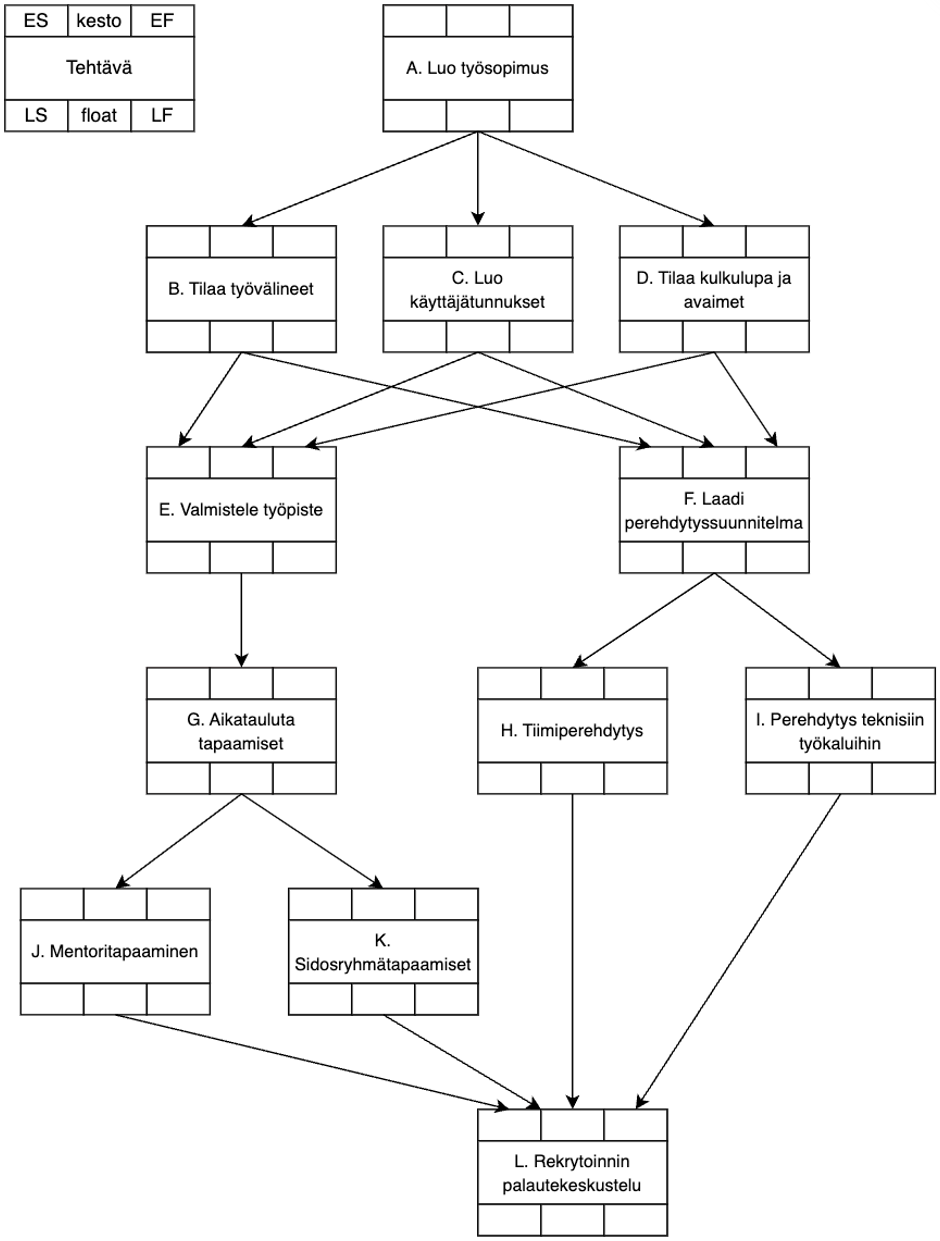
\includegraphics[keepaspectratio]{kuviot/cpm.png}}

}

\caption{\label{fig-cpm}Työntekijän rekrytoinnin prosessi
projektiverkkona kriittisen polun laskentaa varten}

\end{figure}%

\bookmarksetup{startatroot}

\chapter{Prosessiautomaatio ja
tekoäly}\label{prosessiautomaatio-ja-tekouxe4ly}

Tässä luvussa käsitellään liiketoimintaprosessien
automaatiota\sidenote{\footnotesize Tässä luvussa tarvitaan jonkin verran BPMN-kielen
  tuntemista, joten harkitse, luetko tarvittaessa ensin luvun
  \emph{Mallit, mallintaminen ja Business Process Model and Notation}.}.
Tarkastelu keskittyy asiantuntija- ja tietotyön tehtäviin liittyviin
automaatiomahdollisuuksiin, eikä esimerkiksi teollisuus- tai
tuotantoautomaatioon, joilla tarkoitetaan valmistus- ja
tuotantoprosessien sekä niihin liittyvien koneiden ohjaamista ja
valvontaa teknologian avulla (kuva~\ref{fig-manufacturing_line}).

\begin{figure}

\centering{

\pandocbounded{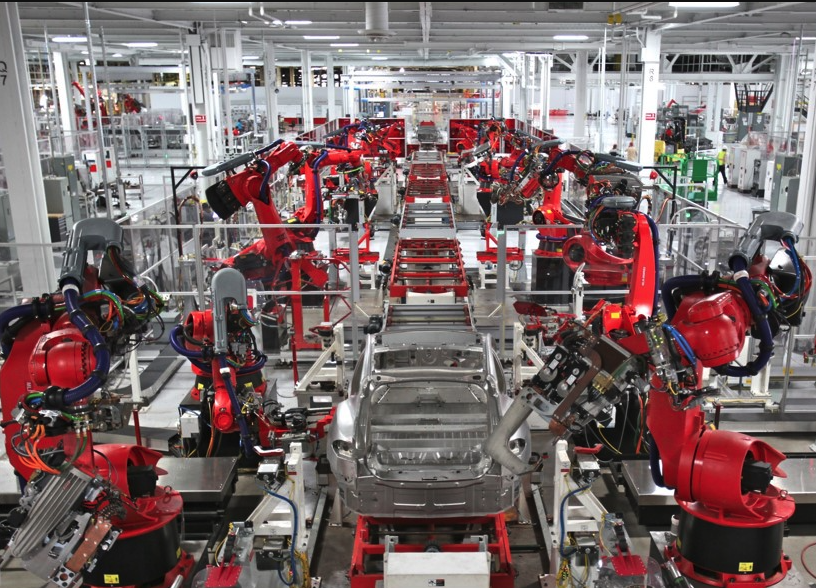
\includegraphics[keepaspectratio]{kuviot/manufacturing_line.png}}

}

\caption{\label{fig-manufacturing_line}Tuotantoteollisuuden
prosessiautomaatiota (CC BY 4.0, Steve Jurvetson)}

\end{figure}%

Lisäksi tarkastellaan tekoälyn mahdollisuuksia prosessien kehittämisessä
ja automaatiossa. Koska tekoälyratkaisujen kehitysvauhti on tällä
hetkellä valtavan nopea, tarkastelu pidetään melko yleisellä tasolla.

Kun prosessi on kuvattu ja analysoitu riittävän tarkasti, voidaan
arvioida automatisoinnin mahdollisuuksia ja kannattavuutta. Seuraavissa
luvuissa käsitellään kolmea liiketoimintaprosessien automaation
toteuttamisen muotoa: työnkulkuautomaatiota, ohjelmistorobotiikkaa sekä
tekoälypohjaisia ratkaisuja.

Edellisten rinnalla ei kannata myöskään unohtaa ohjelmistojen ja
järjestelmien omia mahdollisuuksia, jotka usein voivat olla kevyin ja
edullisin tapa prosessien tehostamiseksi. Tällaisia ovat esimerkiksi
taulukkolaskennan makrot, valmiit raporttipohjat, tallennetut
tietokantakyselyt ja toiminnanohjausjärjestelmän automaattinen täsmäytys
tai hälytykset. Ennen kuin uutta automaatioratkaisua lähdetään
hankkimaan, kannattaa selvittää, onnistuisiko se jo nykyisillä
välineillä.

\section{Työnkulkuautomaatio}\label{tyuxf6nkulkuautomaatio}

Työnkulkuautomaatio (\emph{Workflow Automation}) tarkoittaa toistuviin,
sääntöpohjaisiin prosesseihin kuuluvien tehtävien siirtämistä
ohjelmistojen suoritettavaksi. Työnkulkuautomaatio on tässä luvussa
käsiteltävistä aiheista vanhin: käsitteenä se eli huippukauttaan
1990-luvun lopulla tai 2000-luvun alussa. Toisaalta nykypäivänäkin
esimerkiksi älykäs prosessiautomaatio ja hyperautomaatio edelleen
toteuttavat työnkulkuautomaation tavoitteita ja periaatteita; nyt tosin
hieman kehittyneempien teknologioiden tuella.

Kun prosessimalli esitetään tarkkuudella, joka mahdollistaa prosessin
seuraamisen yksittäisten tehtävien ja tapahtumien tasolla, voidaan sitä
kutsua työnkulkumalliksi.

Tarvitaan tarkkaa ja todellisuudelle uskollista mallintamista, jotta
prosessi -- tai sen työnkulku -- voidaan automatisoida. Ajatellaan
esimerkiksi johonkin prosessiin kuuluvaa tehtävää ''Laske tuotteiden
yhteishinta''. Vaikka tämä tehtävän nimi tai sen sisällön kuvaus on
sinällään ymmärrettävä, ei se vielä riitä siihen, että
automaatiomoottori osaisi suorittaa tehtävän. Työnkulkumallit
vertautuvat työohjeisiin. Jos työohje neuvoo uutta HR-työntekijää
''Käsittele saapunut työhakemus'', ei ohjeella pääse vielä puusta
pitkälle. Paitsi, että ohjeen täytyy jakaa tehtävä pienempiin osiin,
täytyy sen myös kertoa, miten työntekijä voi tietää, että hakemus on
saapunut, mistä hän hakemuksen löytää ja niin edelleen.

Työnkulkumallia (kuva~\ref{fig-pros-workflow}) voidaan ajatella
automaattiseen toimintaan kykenevien järjestelmien työohjeena. Suuriin
kielimalleihin perustuvat ja luonnollisen kielen käsittelyyn kykenevät
järjestelmät saattavat ehkä sopivassa kontekstissa osata tulkita ja
toteuttaa geneerisestikin esitettyjä tehtäviä (kuten ''Käsittele
saapunut työhakemus'') yksityiskohtaisina työnkulkuina, mutta ainakin
toistaiseksi työnkulun mahdollisimman tarkka määritteleminen on
turvallinen valinta.

\begin{figure}

\centering{

\pandocbounded{\includegraphics[keepaspectratio]{index_files/mediabag/kuviot/pros-workflow.pdf}}

}

\caption{\label{fig-pros-workflow}Prosessista työnkulkusovellukseksi
(mukailtu lähteestä Georgakopoulos ym. 1995)}

\end{figure}%

Osa automatisoitavista tehtävistä saattaa nousta esille välittömästi,
kun taas osa voi muodostua vasta työnkulkuspesifikaation ideoinnin,
rakentamisen ja iteroinnin kautta. Oleellista on, ettei työnkulkuja
suunniteltaessa takerruta nykyisiin toimintatapoihin ja niiden
automatisointiin, vaan mietitään, mitä uusia mahdollisuuksia ja
uudenlaisia toimintatapoja teknologiat ja automaatio mahdollistavat.
Tulee myös muistaa, ettei työnkulkujen automatisoinnissa ole useinkaan
mahdollista -- tai edes järkevää -- pyrkiä täysin automatisoituun
toteutukseen. Osa tehtävistä voidaan jättää ihmistoimijoiden
suoritettaviksi \emph{Manual Task}- ja \emph{User Task} -tyyppisinä.

Seuraavassa luvussa käsiteltävän BPMN-kielen (\emph{Business Process
Model and Notation}) ominaisuudet riittävät erinomaisesti
työnkulkumallien laadintaan. BPMN XML -spesifikaatio mahdollistaa myös
prosessimallien automaattisen suorittamisen, joten BPMN toimii paitsi
määrittelykielenä työnkulkumallia luotaessa, myös
runtime-ajoympäristössä suoritettavana työnkulkusovelluksena.
Ohjelmistokokonaisuuksia, jotka mahdollistavat prosessien ja
päätöslogiikan mallintamisen, testaamisen, käyttöönoton ja lopulta
niiden automaattisen suorittamisen, kutsutaan nimellä \emph{Workflow
Engine} tai työnkulkumoottori.

\section{Ohjelmistorobotiikka}\label{ohjelmistorobotiikka}

Ohjelmistorobotiikassa (\emph{Robotic Process Automation}, \emph{RPA})
on kyse sellaisten tehtävien tai prosessien automatisoinnista, joita
suoritetaan tietokoneohjelmistojen käyttöliittymien kautta ja joiden
suorittaminen vaatii tavallisesti runsaasti manuaalista työtä. Tällaiset
tehtävät voivat sisältää vaikkapa tietojen käsittelyä siten, että
lähteenä toimii yksi järjestelmä tai sähköinen dokumentti ja kohteena
toinen. Esimerkiksi sähköpostitse vastaanotettu vikailmoitus voitaisiin
RPA:n avulla kirjata automaattisesti tikettijärjestelmään tai tilaus
tilausrekisteriin.

Ohjelmistorobotiikka saatetaan joskus sekoittaa tekoälyyn, mutta
RPA-ratkaisuilla ei välttämättä tarvitse olla mitään tekemistä tekoälyn
kanssa. Ohjelmistorobotit suorittavat tarkoin määriteltyjä työnkulkuja
seuraten ennalta määriteltyjä ohjeita. Ne toteuttavat tietokoneen
ohjainlaitteiden (kuten näppäimistö ja hiiri) automaatiota, eli ne
pystyvät syöttämään tekstiä ohjelmistojen käyttöliittymiin, liikuttamaan
hiiren kursoria ja vaikkapa painamaan graafisen käyttöliittymän oikeaa
painiketta. Tätä ne eivät tietenkään tee näppäimistöä fyysisesti
näpyttelemällä tai hiirtä liikuttamalla, vaan ohjelmallisesti.
RPA-toteutuksissa voi olla myös konenäköön liittyviä ominaisuuksia,
jolloin ne voivat esimerkiksi etsiä dokumentista tekstiä tai näytöltä
oikean näköisen painikkeen sen sijaan, että niille täytyisi kertoa,
missä koordinaateissa oikea kohde sijaitsee.

Seuraavassa kuvassa (kuva~\ref{fig-mulesoft}) näkyy MuleSoftin \emph{RPA
Builder}\sidenote{\footnotesize https://www.mulesoft.com/platform/rpa} -välineen
käyttöliittymä. Prosessikulku esitetään BPMN-kielellä ja RPA:n
suorittamat tehtävät ovat mallissa \emph{Service Task} -tyyppiä.
Kullekin niistä voidaan määritellä tarkempi tehtävänkulku, jonka aikana
edelleen voidaan hyödyntää RPA Builderin toiminnallisuuksia, kuten
vaikkapa tekstin tunnistaminen dokumentista OCR:n avulla tai muuttujien
käsittely.

\begin{figure}

\centering{

\pandocbounded{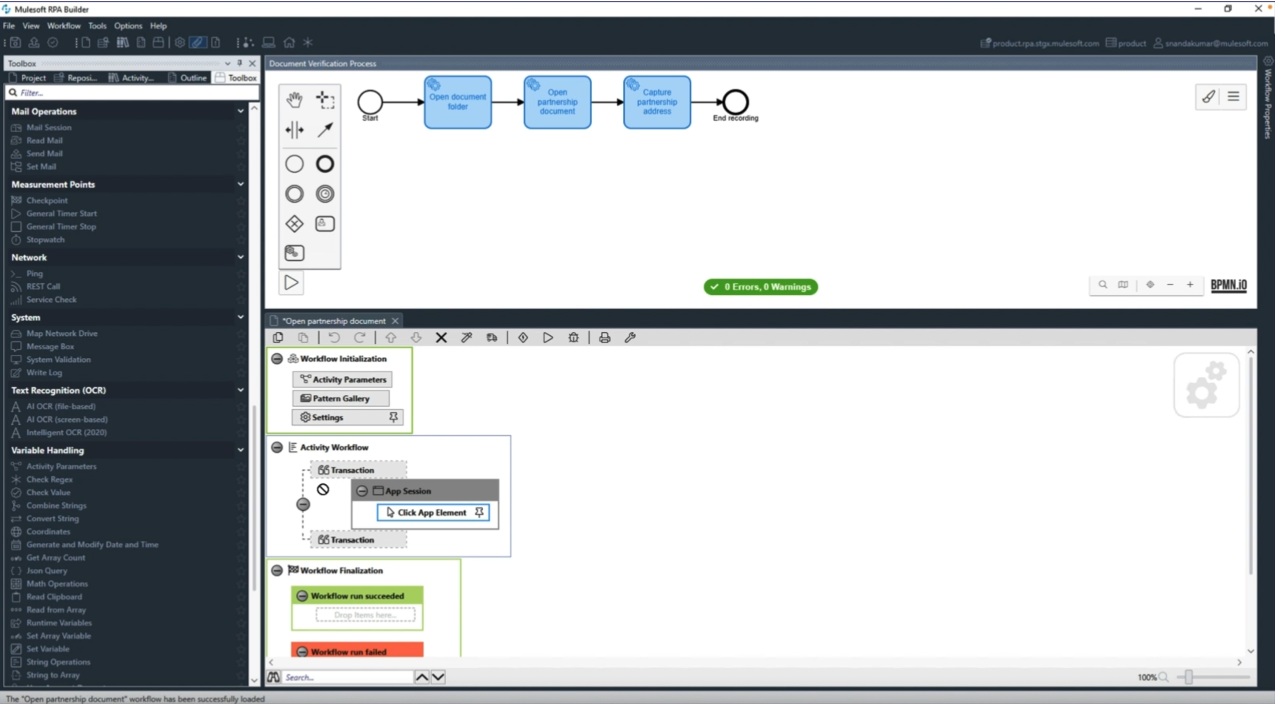
\includegraphics[keepaspectratio]{kuviot/mulesoft-rpa-builder.png}}

}

\caption{\label{fig-mulesoft}MuleSoft RPA Builder on edistynyt
kaupallinen RPA-ympäristö}

\end{figure}%

Alla olevassa kuvassa (kuva~\ref{fig-powerautomate}) on yksityiskohta
\emph{Microsoft Power Automate} -välineellä toteutetusta
prosessikulusta, jossa ohjelmistorobotti hakee työntekijän työmatkan
pituuden lähtöpaikasta työmaalle \emph{Google Maps} -palvelun avulla ja
liittää sen työseurannan \emph{Excel}-taulukkoon. Esimerkki (Kemppainen
2024) osoittaa, kuinka tarkasti ohjelmistorobotin toimintaa voidaan --
ja toisaalta täytyy -- ohjeistaa, kun se operoi graafisen
käyttöliittymän päällä ilman API-rajapintojen käyttöä. Esimerkissä
pyydetään RPA:ta ensin aktivoimaan selaimen Google Maps -ikkuna ja sen
jälkeen kaksoisnapauttamaan näyttöä määritellyssä koordinaattipisteessä.
Sen jälkeen suoritetaan näppäinkomento \emph{Control+C}, joka kopioi
kaksoisnapautuksella valitun tekstin leikepöydälle. Kopioitu teksti
liitetään tämän jälkeen Excel-taulukon oikeaan soluun \emph{Control+V}
-komennolla.

Useat RPA-ratkaisut osaavat myös kutsua ohjelmistorajapintoja. Tällöin
ohjelmistorobotti lukee ja kirjoittaa tietoja sekä käynnistää
ohjelmistojen toimintoja esimerkiksi REST-kutsujen avulla sen sijaan,
että vuorovaikuttaisi niiden kanssa graafisen käyttöliittymän kautta.

\begin{figure}

\centering{

\pandocbounded{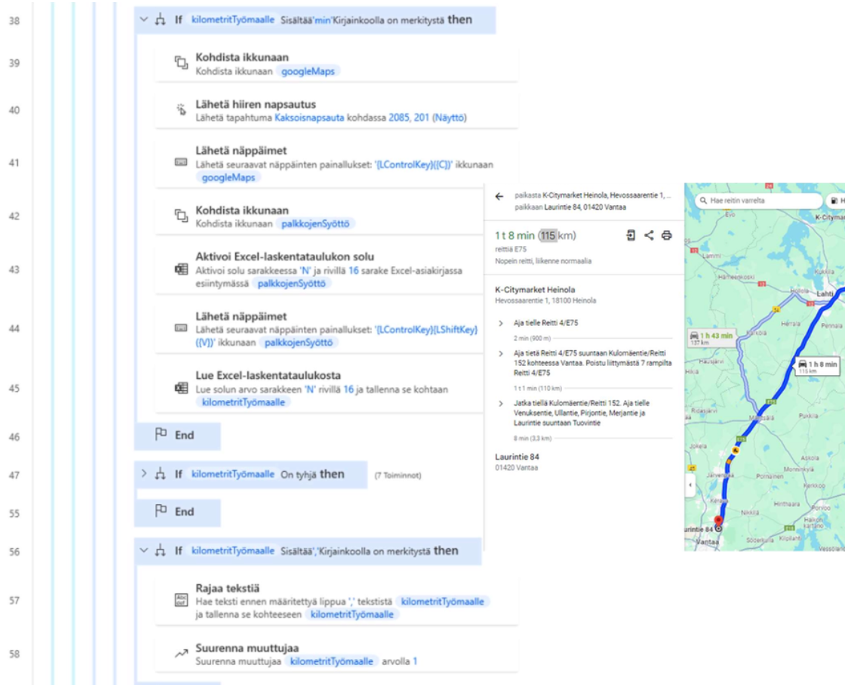
\includegraphics[keepaspectratio]{kuviot/powerautomate.png}}

}

\caption{\label{fig-powerautomate}Esimerkki Microsoft Power Automatella
laaditusta työnkulusta (Kemppainen 2024)}

\end{figure}%

RPA-ratkaisut ovat erittäin tiukkakytkentäisiä. Tämä tarkoittaa, että
niiden rakentaminen edellyttää prosessin suorittamisessa käytettävien
ohjelmistojen ja niiden käyttöliittymien tarkkaa tuntemista. Pienikin
muutos ohjelmiston toimintalogiikassa tai graafisessa käyttöliittymässä,
kuten esimerkiksi tekstikentän tai painikkeen sijainnin muuttuminen, voi
rikkoa työnkulun nykyisen määrittelyn.

Ennen RPA-projektin käynnistämistä kannattaa tehdä huolellinen arviointi
RPA-ratkaisun toteutettavuudesta ja tarpeellisuudesta. Tässä arvioidaan,
voidaanko prosessin toiminnot automatisoida RPA:n avulla ja kuinka
hyödyllistä ja kannattavaa automatisointi on.

Leshob ym. (2018) ovat esittäneet prosessin automaatiokelpoisuuden
arviointiin laskentakaavan (kuva~\ref{fig-rpa-arv1}), joka muodostaa
tulon prosessin tehtävien ohjelmistoavusteisuudesta sekä
sääntöperusteisuudesta. Ensimmäistä tekijää varten selvitetään niiden
tehtävien määrä, joissa ihminen käyttää sovelluksen käyttöliittymää
esimerkiksi valintojen tekemiseen tai tietojen syöttämiseen. Toinen
tekijä muodostuu sellaisten tehtävien osuudesta, jotka toteutetaan
tunnetun säännön tai vakioidun toimintatavan mukaisesti. Toisin sanoen,
mitä useampaan prosessin tehtävistä liittyy sovellusten käyttöä ja mitä
harvempi tehtävistä edellyttää inhimillistä harkintaa tai improvisoitua
päätöksentekoa (esimerkiksi poikkeustilanteissa, joissa automaattinen
päätöksenteko ei ole mahdollista), sitä potentiaalisempi prosessi on
RPA:n avulla automatisoitavaksi.

\begin{figure}

\centering{

\pandocbounded{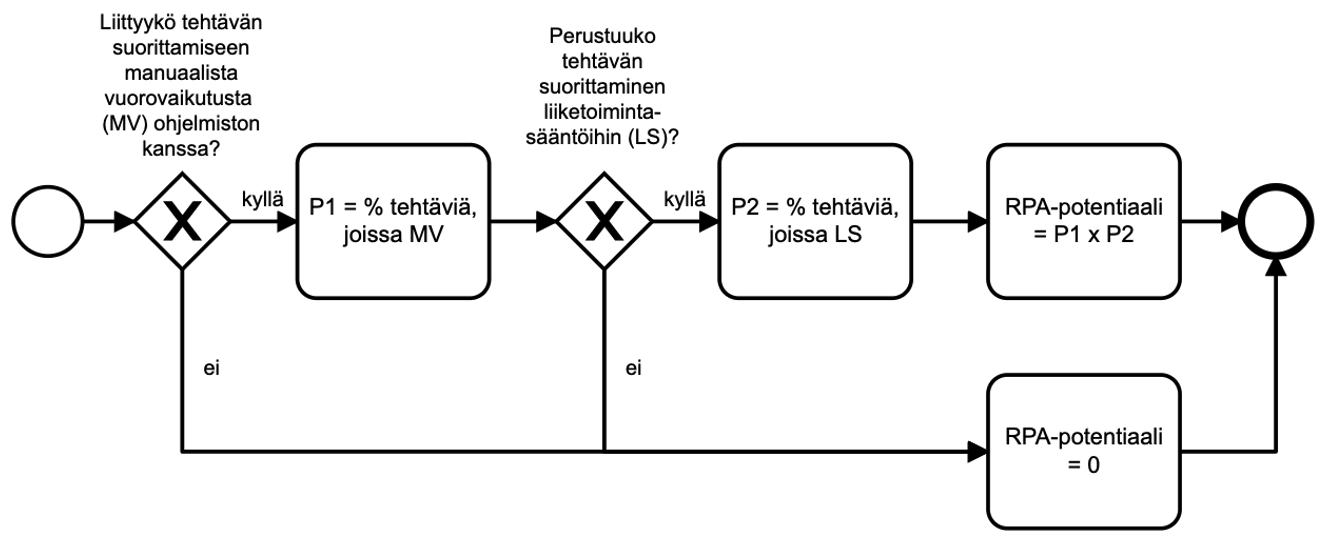
\includegraphics[keepaspectratio]{kuviot/rpa-arv1.png}}

}

\caption{\label{fig-rpa-arv1}Prosessin arviointi RPA-potentiaalin
näkökulmasta}

\end{figure}%

Tarpeellisuutta -- tai relevanssia -- puolestaan arvioidaan prosessin
transaktiomäärien (kuinka usein tehtävä tapahtuu) ja kompleksisuuden
avulla (kuva~\ref{fig-rpa-arv2}). Jälkimmäisen Leshob ym. (2018)
määrittelevät prosessin keston perusteella, mutta joissain tapauksissa
voi olla tarpeen käyttää muitakin parametreja.

\begin{figure}

\centering{

\pandocbounded{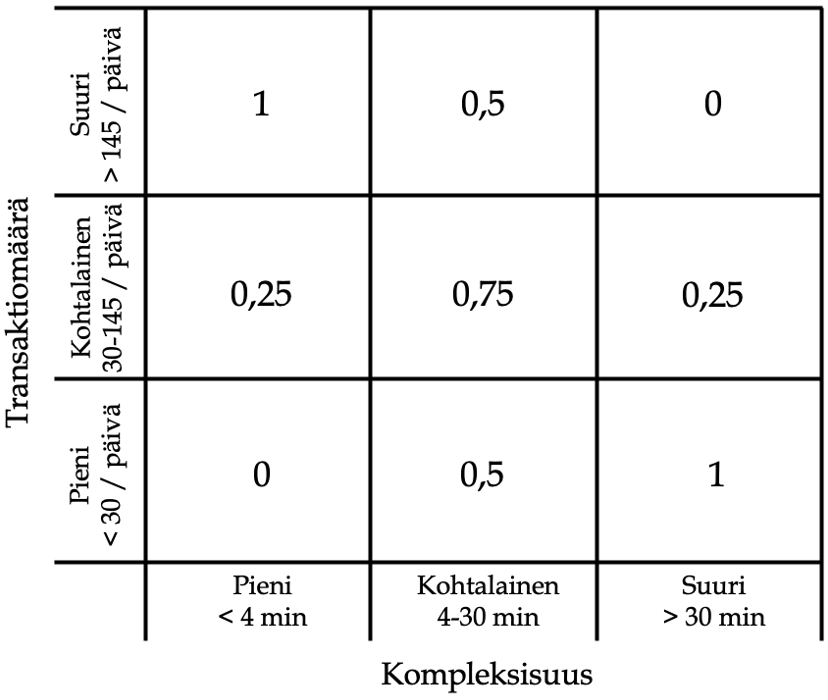
\includegraphics[keepaspectratio]{kuviot/rpa-arv2.png}}

}

\caption{\label{fig-rpa-arv2}Prosessin RPA-relevanssin asteikko}

\end{figure}%

Potentiaalin ja relevanssin perusteella voidaan tehdä kokonaisarvio
siitä, kannattaako prosessille ryhtyä rakentamaan RPA-toteutusta
(kuva~\ref{fig-rpa-arv3}).

\begin{figure}

\centering{

\pandocbounded{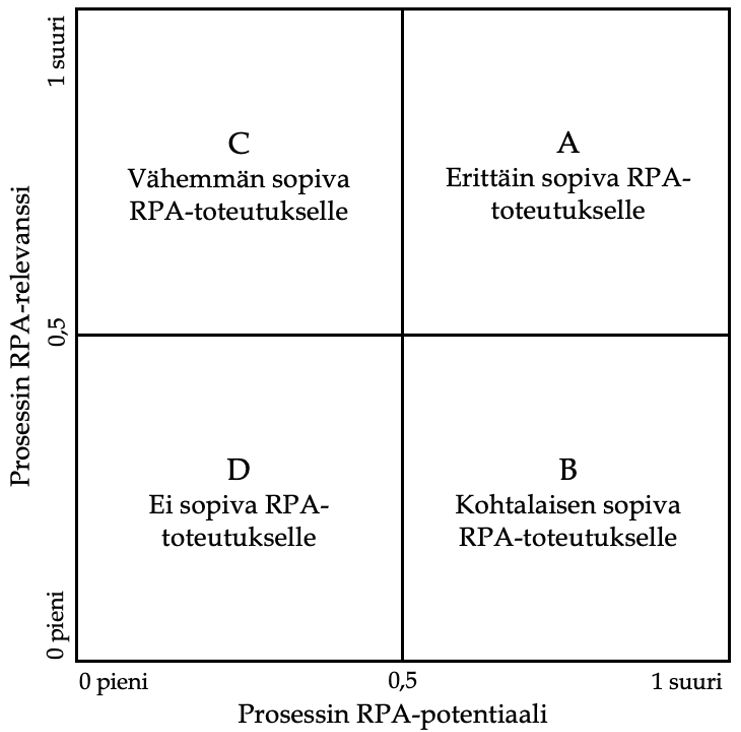
\includegraphics[keepaspectratio]{kuviot/rpa-arv3.png}}

}

\caption{\label{fig-rpa-arv3}Prosessien luokittelu RPA-toteutuksen
kannalta}

\end{figure}%

On syytä arvioida myös RPA-toteutuksen sijoitetun pääoman tuottoa
(\emph{Return On Investment}, \emph{ROI}), takaisinmaksuaikaa tai
kokonaiskustannuksia (\emph{Total Cost of Ownership}, \emph{TCO})
sisältäen toteutuksen välittömät ja välilliset kustannukset sen koko
elinkaaren ajalta. Mikäli prosessin manuaalisen suorittamisen
kustannukset ovat suurillakin tapahtumamäärillä matalat verrattuna
RPA-ratkaisun toteuttamisen hintaan, ei toteutus tietenkään ole
taloudellisesti järkevä. Tulee myös huomioida, että jos prosessin kulku
tai siinä käytettävät ohjelmistot ovat jatkuvasti alttiita muutoksille,
joudutaan myös RPA-toteutusta toistuvasti päivittämään, jolloin sen
elinkaarikustannukset kasvavat.

Onnistuneiden RPA-ratkaisujen hyödyt ovat kuitenkin selkeitä.
Tutkimuksissa (esimerkiksi Shamsuzzoha ja Pelkonen 2025) raportoituja
hyötyjä ovat muun muassa prosessien suorittamisen nopeutuminen,
inhimillisten virheiden poistuminen ja se, että työntekijät voidaan
ohjata tehtäviin, jotka he kokevat mielekkäämmiksi ja joissa tarvitaan
inhimillistä päätöksentekoa tai vuorovaikutusta. Tästä huolimatta
RPA-teknologioihin liitetään kenties aiheellisiakin pelkoja esimerkiksi
joidenkin työtehtävien katoamisesta. Siksi pienissäkin RPA-projekteissa
on syytä huomioida muutosjohtamisen ja sidosryhmäviestinnän näkökulmat.

Edellä on keskitytty pääasiassa prosessien RPA-potentiaalin arviointiin.
Kuten kaikki muutkin liiketoimintaprosessien kehittämiseen liittyvät
tehtävät, myös RPA-ratkaisujen harkinta, arviointi ja rakentaminen
edellyttävät nykyisten prosessien hyvää tuntemista. Prosessien tulisi
olla dokumentoituja ja mielellään esimerkiksi BPMN-kielellä
mallinnettuja. Monet RPA-välineistä toimivat BPMN-mallien perusteella.
Prosesseihin liittyvien liiketoimintasääntöjen tunnistaminen edellyttää
varsin tarkkaakin prosessituntemusta ja RPA-ratkaisun
kustannustehokkuuden arviointi hyötyy suuresti prosesseista kerätystä
mittaritiedosta, kuten suoritustiheys, suoritusaika sekä erilaisten
virhe- ja poikkeustilanteiden määrä.

\begin{longtable}[]{@{}
  >{\raggedright\arraybackslash}p{(\linewidth - 2\tabcolsep) * \real{0.5000}}
  >{\raggedright\arraybackslash}p{(\linewidth - 2\tabcolsep) * \real{0.5000}}@{}}
\caption{RPA-potentiaalin osatekijät (Syed ym.
2020)}\label{tbl-rpa-yhtveto}\tabularnewline
\toprule\noalign{}
\begin{minipage}[b]{\linewidth}\raggedright
Kriteerit
\end{minipage} & \begin{minipage}[b]{\linewidth}\raggedright
Kuvaus
\end{minipage} \\
\midrule\noalign{}
\endfirsthead
\toprule\noalign{}
\begin{minipage}[b]{\linewidth}\raggedright
Kriteerit
\end{minipage} & \begin{minipage}[b]{\linewidth}\raggedright
Kuvaus
\end{minipage} \\
\midrule\noalign{}
\endhead
\bottomrule\noalign{}
\endlastfoot
Sääntöpohjaisuus & Prosessi on pystyttävä kuvaamaan yksiselitteisesti
kaikkien mahdollisten prosessikulkujen osalta. \\
Vähäinen monimutkaisuus & Yksinkertainen ja selkeästi hahmotettavissa
oleva prosessikulku mahdollistaa RPA-toteutuksen. \\
Runsas toistuvuus & Usein toistuvien prosessien automatisointi parantaa
RPA-toteutukseen käytetyn pääoman tuoton todennäköisyyttä. \\
Suuri tapahtumamäärä & Runsaasti tehtäviä sisältävä prosessi usein
maksimoi RPA:n hyötyjen toteutumisen. Tällaiset prosessit ovat
tavallisesti myös rutiininomaisia ja toistuvia. \\
Digitaaliset syötteet & Kaikkien syöte- ja tulostetietojen on oltava
jäsenneltyjä ja digitaalisessa muodossa -- tai digitaaliseen muotoon
muutettavissa. \\
Normalisoitu, jäsennelty, standardoitu ja kypsä prosessi & Mitä paremmin
prosessi tunnetaan ja mitä yksityiskohtaisemmin se on kuvattu, sitä
helpompaa ja vähemmän aikaa vievää RPA-robotin konfigurointi on. \\
Vuorovaikutus useiden ohjelmistojen kanssa & Useita ohjelmistoja
käyttävä prosessi on hyvä RPA:n kohde. Manuaalinen siirtyminen
järjestelmien välillä kasvattaa virheriskiä ja epäjohdonmukaisuutta. \\
\end{longtable}

\section{Hyperautomaatio ja Intelligent Process
Automation}\label{hyperautomaatio-ja-intelligent-process-automation}

Hyperautomaatiolla (\emph{Hyperautomation}) tarkoitetaan erilaisten
automatisoinnin mahdollisuuksien ja niitä tukevien teknologioiden
yhdistelemistä siten, että automaatio voidaan toteuttaa mahdollisimman
laaja-alaisesti. Edellä mainittujen työnkulkuautomaation ja
ohjelmistorobotiikan rinnalla hyperautomaatiossa voidaan käyttää myös
esimerkiksi koneoppimista ja tekoälyä.

Erilaisten teknologioiden soveltamisen lisäksi hyperautomaatiolla
voidaan viitata myös eri toiminta-alueita leikkaavaan ja yhdistävään
automaatioon. Tämä voi esimerkiksi tarkoittaa, että havainnot
markkinoiden muutoksista ohjaavat markkinoinnin prosesseja, joiden
toteuma edelleen vaikuttaa tuotannon prosesseihin, ja joista saatava
reaaliaikainen palaute säätää tarpeen mukaan toimitusketjun prosesseja.

Viime aikoina on ryhdytty käyttämään myös käsitettä \emph{Intelligent
Process Automation} (\emph{IPA}), älykäs prosessiautomaatio, joka
useissa määritelmissä kuulostaa hyvin samankaltaiselta hyperautomaation
kanssa. IPA rikastaa perinteisempiä ohjelmistorobotiikan ratkaisuja
esimerkiksi API-automaation, hahmontunnistuksen, päätösautomaation ja
tekoälyn teknologioilla.

Seuraavassa (kuva~\ref{fig-ipa-esim1}) on esitetty yksinkertaistettu
prosessikulku toimittajalaskun tarkastukselle ja käsittelylle.
Esimerkistä on jätetty pois mahdollisia poikkeustilanteita ja
vaihtoehtoisia kulkuja, joihin tällaisessa prosessissa todellisuudessa
olisi tarpeen varautua. Prosessi alkaa, kun yrityksen tiettyyn
sähköpostiosoitteeseen saapuu toimittajalta lasku PDF-muodossa.
Ostoassistentti tallentaa laskun verkkolevylle ja sen jälkeen tarkastaa
laskun oleelliset tiedot. Sitten hän varmistaa ERP-järjestelmästä, että
laskutetut tuotteet on vastaanotettu. Tämän jälkeen hän toimittaa laskun
hyväksyttäväksi oikealle henkilölle, esimerkiksi yksikön johtajalle tai
hankintavastaavalle. Kun lasku on hyväksytty, ostoassistentti kirjaa sen
tiedot talousjärjestelmään maksettaviin laskuihin.

\begin{figure}

\centering{

\pandocbounded{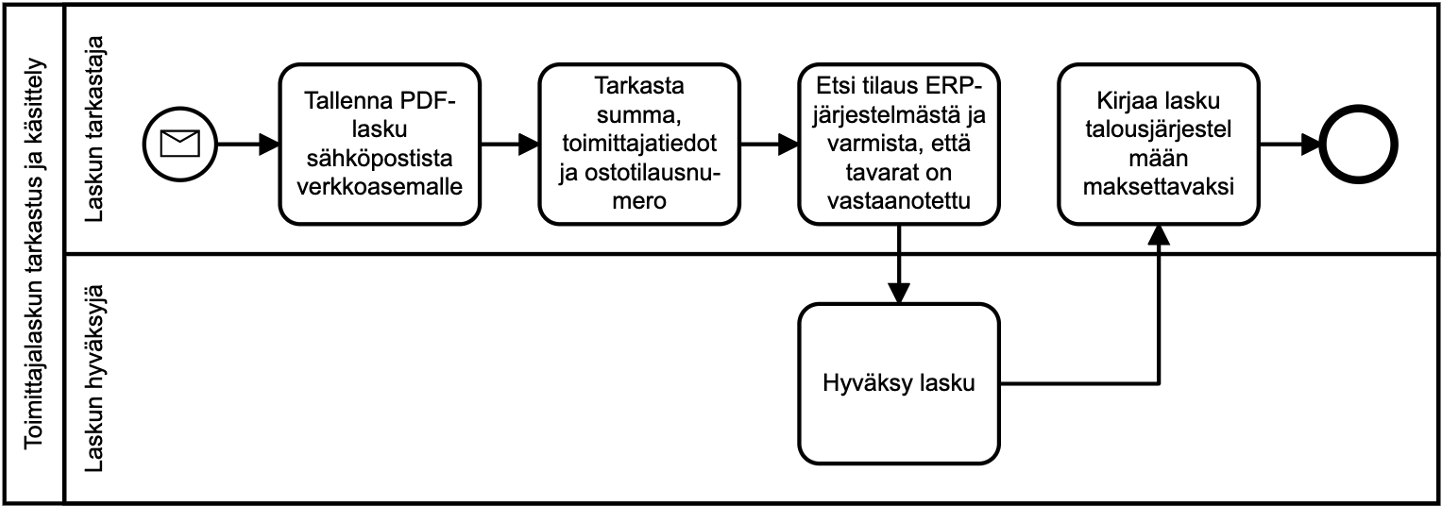
\includegraphics[keepaspectratio]{kuviot/ipa-esim1.png}}

}

\caption{\label{fig-ipa-esim1}Yksinkertainen toimittajalaskun
tarkastuksen ja käsittelyn prosessi}

\end{figure}%

Seuraavassa (kuva~\ref{fig-ipa-esim2}) edellinen prosessi on hahmoteltu
hyperautomaatiototeutuksen muotoon. Uimaradat on varattu
prosessimallissa nyt kolmelle teknologialle, joita prosessin
suorittamisessa hyödynnetään. Työnkulkualusta vastaa prosessikulun
yleisestä ohjaamisesta ja suorittamisesta. Prosessin aikana se ohjaa
osan tehtävistä muiden automaatioteknologioiden suoritettavaksi sekä
kutsuu ERP-järjestelmää.

\begin{figure}

\centering{

\pandocbounded{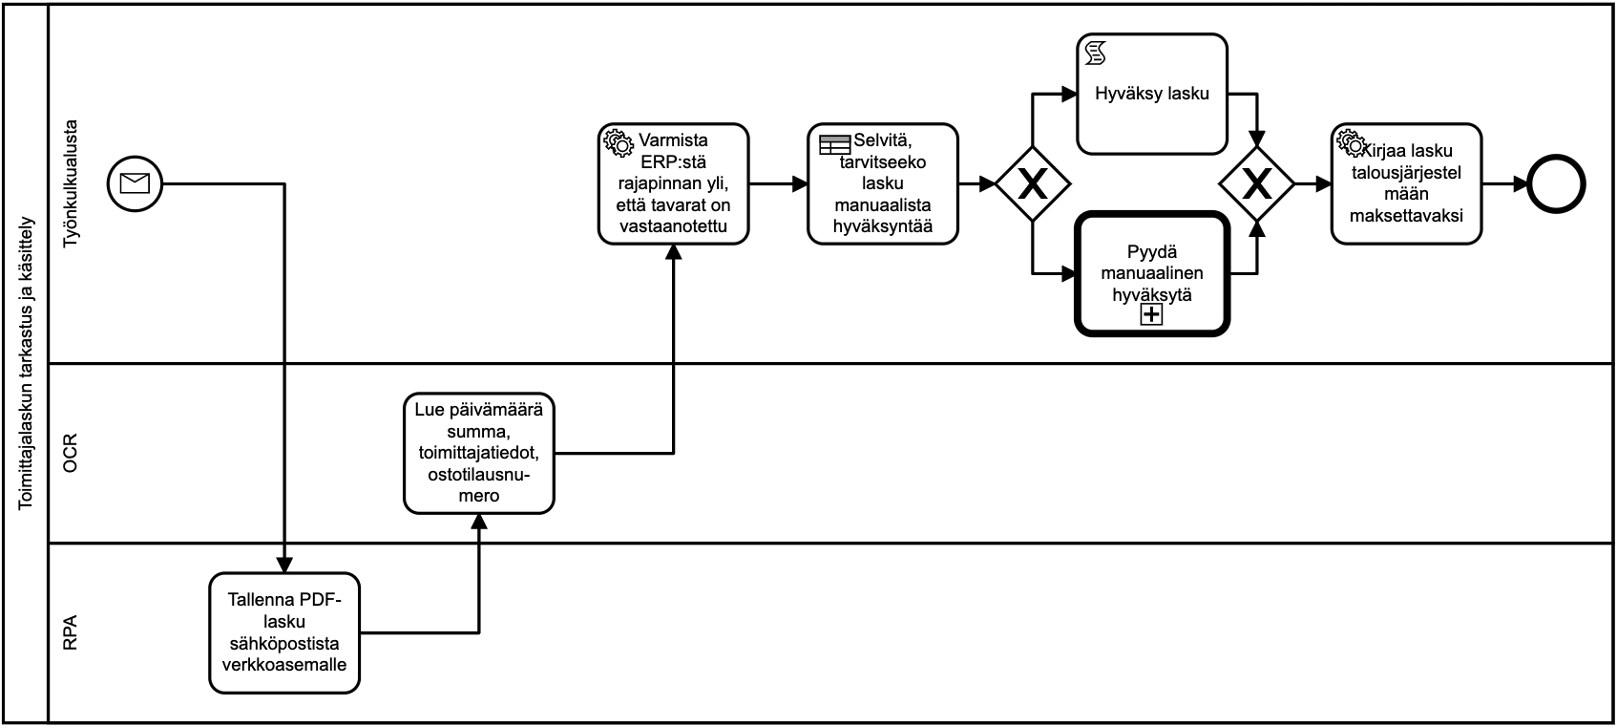
\includegraphics[keepaspectratio]{kuviot/ipa-esim2.png}}

}

\caption{\label{fig-ipa-esim2}Yksinkertaisen toimittajalaskun
tarkastuksen ja käsittelyn prosessi hyperautomaationa}

\end{figure}%

Toimittajalaskun saavuttua sähköpostiin, työnkulkualusta kutsuu
ohjelmistorobottia, joka etsii laskun ja tallentaa sen verkkoasemalle.
Ohjelmistorobotti kutsuu OCR-toimintoa (\emph{Optical Character
Recognition}), joka lukee hahmontunnistusta hyödyntäen laskulta
relevantit tiedot ja palauttaa ne takaisin työnkulkualustalle
prosessimuuttujina. Työnkulkualusta kysyy ERP-järjestelmältä
(\emph{Service Task}) API-rajapinnan yli, ovatko tilaukseen liittyvät
tuotteet saapuneet ja lasku siltä osin valmis maksettavaksi. Seuraavaksi
työnkulkualusta päättelee päätöstaulun (\emph{Business Rule Task})
avulla, voidaanko lasku hyväksyä automaattisesti. Mikäli se on
mahdollista, lasku hyväksytään prosessikulkuun liitetyllä
ohjelmakoodilla (\emph{Script Task}). Mikäli lasku jostain syystä --
esimerkiksi korkean hinnan vuoksi -- tarvitsee manuaalisen hyväksynnän,
hyväksyntä pyydetään kutsumalla aliprosessia (\emph{Call Activity}).
Lopuksi hyväksytyn laskun tiedot viedään automaattisesti (\emph{Service
Task}) talousjärjestelmään maksettavien laskujen joukkoon.

Koko prosessi voidaan käsitellä ilman manuaalista työtä, ellei laskun
hyväksyntä jostain syystä sitä edellytä. Prosessin läpinäkyvyys ja
nopeus paranevat, samoin kuin unohdusten ja inhimillisten virheiden
määrä vähenee.

\section{Tekoäly prosessiautomaatiossa}\label{sec-tekoaly-automaatiossa}

Hyperautomaation ratkaisuissa tekoälyä käytetään lähinnä yksittäisten
tehtävien suorittamisessa, esimerkiksi hahmontunnistus dokumenttia
luettaessa tai päätösautomaatiota täydentävä koneoppiminen. Suurten
kielimallien yleistyminen on kuitenkin tuomassa tekoälyn
prosessiautomaatioon myös laajamittaisemmin. Se voi tietyissä
tilanteissa ottaa vastuulleen kokonaisia prosessikulkuja tai jopa
päättää, missä järjestyksessä ja millä keinoin prosessiin kuuluvat
tehtävät suoritetaan.

Autonomiset tekoälyagentit pystyvät jo nykyisin suorittamaan vaativiakin
tehtäviä itsenäisesti ja ilman ohjausta. Useista keskenään
vuorovaikuttavista agenteista koostuvat järjestelmät pystyvät
suorittamaan monimutkaisia tehtäväsarjoja -- eli prosesseja.
Lähitulevaisuudessa saatamme olla tilanteessa, jossa prosessimalliksi
riittää BPMN:n \emph{Ad-hoc} -prosessin kaltainen sekalainen joukko
irrallisia tehtäviä tai jopa ainoastaan halutun lisättyä arvoa tuottavan
lopputuloksen ilmoittaminen.

Vuoden 2026 aikana saatiin lukea useista ``välikohtauksista'', joissa
tekoälyagenttien kerrottiin ``karanneen'' ja murtautuneen esimerkiksi
terveydenhuollon järjestelmiin\sidenote{\footnotesize https://yle.fi/a/74-20237506}\textsuperscript{,}\sidenote{\footnotesize https://yle.fi/a/74-20247954}.
Agentit eivät tietenkään toimi näin ilkeyttään, vaan etsiessään tietoa,
jota ne tarvitsevat niille annetun tehtävän ratkaisemiseksi. Joka
tapauksessa autonomisen tekoälyn käyttöön prosessiautomaatiossa
kannattaa vielä ainakin toistaiseksi suhtautua varauksella ja
harkinnalla.

Kuten edellä todettiin, tekoälyratkaisujen kehitysvauhti on tällä
hetkellä niin suuri, että yksittäisiä tuotteita tai teknologioita
koskevat havainnot vanhenevat nopeasti. Tarkastelu pidetään seuraavassa
siksi periaatteiden tasolla.

\subsection{Tekoäly prosessin yksittäisissä
tehtävissä}\label{tekouxe4ly-prosessin-yksittuxe4isissuxe4-tehtuxe4vissuxe4}

Tekoälyä, kuten kielimalleja, voidaan ajatella yhtenä prosessin
tehtävien suorittajana muiden joukossa. Edellä esitetyssä
laskunkäsittelyn prosessissa (kuva~\ref{fig-ipa-esim2}) OCR-toiminto
luki laskulta tiedot ja palautti ne työnkulkualustalle
prosessimuuttujina. Perinteinen OCR-ratkaisu toimii, kun laskut ovat
rakenteeltaan vakioituja ja tiedot löytyvät aina suurin piirtein
samoista kohdista. Toimittajia saattaa kuitenkin olla useita, ja
jokaisella voi olla omanlaisensa laskupohja. Joskus viitenumero on
oikeassa yläkulmassa, joskus alatunnisteessa, ja joskus lasku on
liitetty sähköpostiin valokuvana ruttuisesta paperista.

Tekoälyllä on valmiuksia tulkita vaihtelevaa ja puolirakenteista
aineistoa huomattavasti sääntöpohjaista tunnistusta joustavammin. Sille
voidaan antaa ohjeeksi esimerkiksi ''Poimi laskulta toimittajan nimi,
Y-tunnus, laskun summa, eräpäivä ja tilausnumero'', ja se palauttaa
tiedot työnkulkualustalle samaan tapaan kuin OCR-toiminto aiemmin.
Prosessimallissa tämä voisi olla \emph{Service Task} -tyyppinen tehtävä,
jossa kutsutaan kielimallia rajapinnan yli, tai oma uimarata muiden
automaatioteknologioiden rinnalla.

Vastaavia tehtäviä löytyy lähes kaikista asiantuntija- ja tietotyön
prosesseista: palvelupyyntöjen luokittelu ja ohjaus eteenpäin, pitkien
asiasisältöjen tiivistäminen, rakenteettoman tiedon muuttaminen
rakenteiseen muotoon, tarvittavat tyyppimuunnokset siirrettäessä tietoja
järjestelmien välillä ja niin edelleen.

Tällaisissa ratkaisuissa prosessin kulku on edelleen tarkasti
mallinnettu ja työnkulkualustan ohjaama. Tekoäly ainoastaan muuttaa
joidenkin tehtävien toteutustapoja. Tämä on varsin hallittava ja
turvallinenkin tapa tuoda tekoälyä osaksi prosessien suorittamista.
Työnkulku edelleen määrittelee, mitä tehdään ja missä järjestyksessä, ja
tekoäly toteuttaa vain sille osoitetun osan.

On syytä kuitenkin muistaa, etteivät kielimallit toimi kuten perinteinen
ohjelmakoodi. Ne eivät ole deterministisiä eli sama syöte ei välttämättä
tuota joka kerta täsmälleen samaa lopputulosta. Kielimallit saattavat
pahimmillaan myös tuottaa uskottavan näköisiä, mutta virheellisiä
vastauksia.

Tekoälyn tuottamat tiedot kannattaa mahdollisuuksien mukaan tarkistaa
automaattisesti. Esimerkiksi laskun summaa voidaan verrata
ERP-järjestelmän tilaustietoihin tai yritystunnuksen oikeellisuus
voidaan varmistaa toimittajarekisteristä. Mikäli tiedot eivät täsmää,
voi prosessi ohjata laskun ihmisen käsiteltäväksi.

Průcha ym. (2025) vertasivat UiPath RPA\sidenote{\footnotesize https://www.uipath.com/rpa/robotic-process-automation}
-ohjelmistorobotiikkaratkaisua ja kielimalliagenttia kolmessa
tehtävässä: tiedonsyötössä, seurannassa ja dokumenttien tietojen
poiminnassa. Tutkimuksen mukaan ohjelmistorobotti oli toiminnassaan
nopeampi ja luotettavampi. Sen sijaan agenttiratkaisujen kehitysaika oli
lyhyempi ja ne selvisivät käyttöliittymän muutoksia huomattavasti
RPA-ratkaisuja paremmin.

\subsection{Agenttinen tekoäly}\label{agenttinen-tekouxe4ly}

Aiemmin todettiin, että kielimalleihin perustuvat järjestelmät saattavat
sopivassa kontekstissa pystyä tulkitsemaan ja toteuttamaan
geneerisestikin esitettyjä tehtäviä, kuten ''Käsittele saapunut
työhakemus''. Tätä voidaan kutsua agenttiseksi tekoälyksi (\emph{Agentic
AI}). Tekoälyagentille ei anneta yksityiskohtaista kuvausta prosessin
kulusta, vaan prosessin tavoite sekä joukko työkaluja, joita se saa
käyttää tavoitteen saavuttamiseksi. Työhakemuksen käsittelyyn liittyviä
työkaluja voivat olla hakemusjärjestelmä, kalenteri ja sähköposti.
Agentti päättää itsenäisesti, mitä tehtäviä se suorittaa ja missä
järjestyksessä, mitä tietoja se hakee ja milloin tavoite on saavutettu.
Useampi agentti voi myös toimia yhdessä siten, että kullakin on
prosessissa oma erikoistunut roolinsa ja ne välittävät tehtäviä ja
tietoja toisilleen.

Ye ym. (2023) kutsuvat tätä kehitystä siirtymäksi ohjelmistorobotiikasta
agenttiseen prosessiautomaatioon (\emph{Agentic Process Automation}).
Kielimalliagentit sekä rakentavat työnkulun ihmisen antamista ohjeista
että tekevät sen suorittamisen aikana tarvittavat päätökset. Työnkulku
koordinoi erikoistuneita agentteja, jotka suorittavat prosessin
tehtäviä.

Ero perinteiseen prosessiautomaatioon on merkittävä. Ohjelmistorobotti
suorittaa tarkoin määriteltyjä työnkulkuja ja voi rikkoutua, jos
käyttöliittymän painike vaihtaa paikkaa. Työnkulkualusta puolestaan
seuraa tarkoin määriteltyä ja mallinnettua prosessikulkua. Agentti voi
muodostaa oman työnkulkunsa jokaista tapausta varten. Toisaalta tämä
tekee agenteista joustavia ja ne pystyvät käsittelemään
poikkeustilanteita, joita ei välttämättä olisi osattu etukäteen
ennakoida ja mallintaa työnkulkuun. Toisaalta samasta syystä agentin
toimintaa on vaikeampi ennakoida, testata ja valvoa.

BPMN-kielen \emph{Ad-hoc}-aliprosessi sopii agenttien kuvaamiseen varsin
luontevasti -- vaikka sitä tuskin alun perin tähän tarkoitukseen on
suunniteltu. Se on joukko tehtäviä, jotka voidaan suorittaa tai olla
suorittamatta, ja joiden suoritusjärjestystä ei ole ennalta määrätty.
Agentin toimintaa voidaan siis kuvata prosessimallissa
Ad-hoc-aliprosessina, jonka sisällä agentti valitsee käytettävissä
olevista tehtävistä ja välineistä tilanteeseen sopivat. Ympäröivä
prosessi on kuitenkin tarkasti mallinnettu ja hallittu. Se määrää,
milloin agentille annetaan tehtävä, mitä sen tulee tehtävän
suoritettuaan palauttaa, ja mihin pääprosessin kulku sen jälkeen etenee.
Osa työnkulkualustojen toimittajista onkin jo ryhtynyt tukemaan
tekoälyagenttien orkestrointia BPMN-prosessien osana.

Agenttiseen tekoälyyn liittyy kuitenkin periaatteellisempi haaste.
Generatiivisten tekoälyjen ja suurten kielimallien toiminta on siis
epädeterminististä ja muistuttaa mustaa laatikkoa. Agentille voidaan
antaa tavoite ja seurata sen tekemiä toimenpiteitä. Emme kuitenkaan
välttämättä tiedä, millaisen päättelyn tuloksena se päätyi juuri näihin
toimenpiteisiin tai edes sitä, tuottivatko ne oikeita lopputuloksia.

Tämä palauttaa meidät takaisin alkuun ja ongelmaan, jota
liiketoimintaprosessien hallinnalla on pyritty ratkaisemaan:

\begin{quote}
Sumean linssin läpi tarkasteltuna prosessi voi näyttäytyä mustana
laatikkona: jotain menee sisälle, joitain asioita tapahtuu, ja lopuksi
laatikosta tulee jotain ulos. Joskus tämä vertaus saattaa valitettavasti
vastatakin organisaatioiden kyvykkyyttä ymmärtää omia prosessejaan.
\end{quote}

Prosessien johtamisen näkökulmasta tämä on vähintään paradoksaalista --
kenties kestämätöntäkin. Prosesseja mallinnetaan, jotta toiminta olisi
läpinäkyvää, toistettavaa ja kehitettävissä. Jos prosessin jokin
keskeinen osa suoritetaan tavalla, jota kukaan ei täysin tunne, myös
prosessin mittaaminen vaikeutuu ja konkreettiset edellytykset jatkuvalle
parantamiselle katoavat.

Työnkulun mahdollisimman tarkka määritteleminen on ainakin toistaiseksi
turvallinen valinta silloin, kun prosessi on kriittinen, säännelty tai
sen virheillä voi olla merkittäviä seurauksia. Agentit sopivat
tilanteisiin, joissa tapaukset vaihtelevat paljon, virheiden seuraukset
ovat korjattavissa ja joissa lopputuloksen tarkistaminen on helpompaa
kuin itse työn tekeminen.

\subsection{Ihminen silmukassa ja tekoälyn
hallinta}\label{ihminen-silmukassa-ja-tekouxe4lyn-hallinta}

Kun tekoäly osallistuu prosessin suorittamiseen, voi nousta kysymys
siitä, kuka on vastuussa sen mahdollisesti tekemistä virheistä.
Tosiasiassa vastuu säilyy aina prosessia suorittavalla organisaatiolla
ja viime kädessä prosessin omistajalla. Siksi tekoälyä hyödyntäviin
prosesseihin tulee suunnitella kohtia, joissa ihminen tarkastaa,
hyväksyy tai korjaa tekoälyn tuotoksen. Tätä kutsutaan \emph{Human in
the Loop}- tai ihminen silmukassa -periaatteeksi.

Laadittaessa prosessimallit BPMN-kielellä, on ihminen helppo lisätä
silmukkaan: tekoälyn suorittaman tehtävän jälkeen prosessiin lisätään
esimerkiksi \emph{User Task}, jossa ihminen tarkastaa tuloksen ennen
prosessin jatkumista.

Kaikkea ei kuitenkaan ole järkevää tarkastaa. Jos jokainen tekoälyn
käsittelemä lasku käydään vielä ihmisen toimesta läpi, on automaation
hyöty jokseenkin kyseenalainen. Tarkastus voidaankin ehtoperusteisesti
kohdistaa esimerkiksi suuriin summiin, epätavallisiin tapauksiin tai
sellaisiin, joissa tekoäly ilmoittaa olevansa epävarma lopputuloksesta.
Lisäksi satunnaisotannalla voidaan seurata, pysyykö tekoälyn toiminnan
laatu hyväksyttävällä tasolla.

Ihmisen tekemään tarkastukseen liittyy haasteitakin. Tekoälyn tuottama
teksti tai muu tulos on usein uskottavan näköistä, ja virheet voivat
jäädä huomaamatta. Mitä harvemmin tekoäly erehtyy, sitä helpommin
tarkastaja alkaa luottaa siihen, eikä tarkastus enää ole välttämättä
todellinen. Lisäksi tarkastaminen on työlästä; useissa tehtävissä
työläämpää kuin tehtävän suorittaminen. Ihminen silmukassa -periaate
toimii vain, kun tarkastukselle on varattu riittävästi aikaa ja
tarkastajalla tehtävää koskevaa asiantuntemusta.

Myös nykyinen lainsäädäntö asettaa reunaehtoja tekoälyn käyttämiselle
prosessiautomaatiossa. Suomessa julkisen hallinnon automaattista
päätöksentekoa koskeva lainsäädäntö tuli voimaan keväällä
2023\sidenote{\footnotesize Hallituksen esitys HE 145/2022,
  https://www.finlex.fi/fi/hallituksen-esitykset/2022/145}. Se kieltää
automaattisen päätöksenteon tilanteissa, jotka edellyttävät viranomaisen
harkintavaltaa, perustuvat yksilölliseen arviointiin tai olosuhteiden
kokonaisvaltaiseen punnintaan, tai joihin liittyy merkittäviä
vaikutuksia yksilön oikeuksiin tai velvollisuuksiin.

Euroopan unionin tekoälysäädös\sidenote{\footnotesize Euroopan parlamentin ja
  neuvoston asetus (EU) 2024/1689 tekoälyä koskevista
  yhdenmukaistetuista säännöistä.
  https://eur-lex.europa.eu/eli/reg/2024/1689/oj} (\emph{EU AI Act})
puolestaan luokittelee tekoälyjärjestelmiä niiden riskitason
perusteella. Esimerkiksi rekrytointiin, koulutukseen tai julkisiin
palveluihin liittyvät tekoälysovellukset voivat kuulua korkean riskin
luokkaan, jolloin niiden käytölle asetetaan erityisiä vaatimuksia muun
muassa ihmisen suorittaman valvonnan, dokumentoinnin ja läpinäkyvyyden
osalta. Edellä mainittu ''Käsittele saapunut työhakemus'' -agentti ei
siis olisi ainoastaan tekninen, vaan myös juridinen kysymys.

Tekoälyn tuominen osaksi prosesseja ei siis ole pelkästään teknologioita
koskeva kysymys. Kuten Outi Sivonen johdannossa lainatussa
kirjoituksessaan totesi, tekoälyn käyttöönotossa eivät muutu vain
yksittäiset työtehtävät, vaan myös prosessit ja niiden johtaminen.
Automaatio on vasta ensimmäinen askel. On liian helppoa tehdä tekoälyn
ja automaation avulla nopeammin sitä, mitä jo nyt tehdään -- myös
silloin, kun sitä ei oikeastaan kannattaisi tehdä ollenkaan. Siksi
tekoäly ei muuta prosessien kehittämisen perusperiaatteita: ensin tulee
miettiä, mitä arvoa prosessi tuottaa ja kenelle, ja vasta sitten sitä,
miten prosessi kannattaa toteuttaa.

\bookmarksetup{startatroot}

\chapter{Harjoitustehtäviä}\label{harjoitustehtuxe4viuxe4}

\section{Tehtävä 1}\label{tehtuxe4vuxe4-1}

Jos tunnemme riittävän tarkasti prosessikulun, jolla yritys lähettää
vuosittain 3 500 asiakkaalleen toimitusjohtajan käsin kirjaileman
joulutervehdyksen postikortilla, tiedämme, että yhdeltä työntekijältä
kuluu postimerkkien liimaamiseen noin 35 000 sekuntia eli noin 9 tuntia
45 minuuttia. Sopivan lyhyine taukoineen tämä vastaa noin puoltatoista
työpäivää. Jos postimerkkien liimaamiseen osallistuisikin neljä
työntekijää, olisi urakka hoidettu noin 2,5 tunnissa. Säästäisimme
aikaa, mutta nyt yksi prosessin vaihe sitoisi neljä työntekijää eli
kuluttaisi hetkellisesti neljä kertaa enemmän henkilöstöresurssia.
Vaiheen tarvitsemat henkilötyötunnit säilyisivät kokonaisuudessaan
kuitenkin tietysti suurin piirtein ennallaan.

Joulukorttiprosessiasiantuntija saattaisi tässä vaiheessa myös harkita
sellaisia joulukortteja, joiden postimaksu on valmiiksi maksettu.
Yrityksen logolla varustettu joulukortti maksaa 50 senttiä ja siihen
postimerkki 1,50 euroa. Näin ollen yksi postitusvalmis kortti
postimerkkeineen maksaa kaksi euroa ja koko 3 500 kortin nippu 7 000
euroa. Punaisen Ristin joulukortti, jossa postimaksu on valmiiksi
maksettu, maksaa 3,40 euroa kappaleelta, joten kortit maksaisivat
yhteensä 11 900 euroa. Postimerkit itse liimaamalla yritys siis
säästäisi joulukorteissa ja postimerkeissä vuosittain 4 900 euroa. Ei
tule kuitenkaan unohtaa postimerkkien liimaamiseen kuluvaa työaikaa,
joka oli siis vajaat kymmenen tuntia.

Jos olisimme mittaroineet aiempien vuosien joulukorttiprosessia
erityisen tarkasti, saattaisimme myös tietää, kuinka moni postimerkki
repeää vihkosta irrotettaessa liimauskelvottomaan kuntoon, kuinka moni
joulukortti on ollut vekillä jo saapuessaan tai ruttaantuu merkkien
liimaamisen aikana ja niin edelleen. Nämä ja monet muut tiedot, tai
jonkinlaiset arviot niistä, voisimme myös syöttää prosessisimulaattoriin
optimaalista tehokkuutta etsittäessä.

Sen ainakin tiedämme, että merkkien liimaamiseen osallistuvan henkilön
tuntipalkka on 25 euroa, joten välittömät palkkakustannukset yhdeksän
tunnin liimausurakasta ovat noin 225 euroa. Palkkakustannuksiin täytyy
tietenkin lisätä muut kustannukset, kuten työnantajan
sosiaaliturvamaksut, työterveyskulut, vakuutukset ja muut vastaavat.
Nämä lisäkulut ovat tavallisesti vähintään 30 prosenttia palkasta, joten
postimerkkien liimaamisen kustannukset nousisivat nyt lähelle 300 euroa.
Postimerkit itse liimaamalla prosessin kustannukset olisivat kuitenkin
edelleen noin 4 600 euroa matalammat kuin Punaisen Ristin joulukortteja
käytettäessä. Tässä ei kuitenkaan tule unohtaa, että työntekijä tai
työntekijät, jotka käyttävät tunteja postimerkkien liimaamiseen, ovat
sen ajan poissa varsinaiseen toimenkuvaansa liittyvien tehtävien
hoitamisesta. Mikä tuottotappio tästä seuraa, ja mitkä ovat sen
kokonais- ja mahdolliset heijastuskustannukset, riippuu lukuisista
tekijöistä. Myös nämä tekijät tulisi tuntea, jotta prosessille voidaan
valita ideaali toteutustapa.

Ja mikäli prosessiasiantuntijamme ei olisi vielä saanut tarpeekseen,
voisi hän seuraavaksi yrityksen PR-vastaavan kannustamana ryhtyä
selvittämään, arvottavatko asiakkaamme joulukorteissaan korkeammalle
yrityksemme logon vai Punaisen Ristin logon. Jälkimmäinen voisi kenties
viestiä asiakkaille yrityksen vastuullisesta arvopohjasta. Mutta
johtavatko joulukortit palaaviin asiakkaisiin ja lisämyyntiin? Tuottaako
joulukorttiprosessi lopulta lainkaan arvoa vai ainoastaan kustannuksia?

Pohdi edellisen perusteella seuraavia kysymyksiä:

\begin{itemize}
\tightlist
\item
  Mitkä ovat prosessin kriittiset vaiheet ja mahdolliset pullonkaulat?
\item
  Miten vaiheiden ajoitus ja resursointi vaikuttavat koko prosessin
  läpimenoaikaan?
\item
  Milloin on perusteltua käyttää useampia työntekijöitä yhden
  työntekijän pidemmän suorituksen sijaan?
\item
  Miten mittaisit, tuottaako prosessi yritykselle arvoa?
\end{itemize}

\section{Tehtävä 2}\label{tehtuxe4vuxe4-2}

Selvitä, mitä tarkoittaa digitaalinen kaksonen eli digital twin.
Liittyykö se prosessisimulointiin, ja jos liittyy, niin miten?

\section{Tehtävä 3}\label{tehtuxe4vuxe4-3}

Seuraavassa on esimerkki asiakastilauksia käsittelevässä roolissa
työskentelevän henkilön haastattelusta. Haastattelu liittyy
elektroniikkatuotteita myyvän verkkokaupan tilauskäsittelyprosessiin.
Tutustu haastattelun transkriptioon ja laadi vuokaavio tai BPMN-malli
prosessin nykytilasta. Nosta esille tunnistettavat kehittämiskohteet ja
mieti, miten niihin voitaisiin reagoida.

\textbf{Milloin prosessi käynnistyy tai mikä sen käynnistää?}

Prosessi käynnistyy, kun asiakas tekee tilauksen verkkokaupassamme. Tämä
voi tapahtua milloin tahansa, koska verkkokauppa toimii 24/7 ympäri
vuoden.

\textbf{Kuinka usein prosessi suoritetaan?}

Päivittäin käsitellään noin 300 tilausta ja viikossa määrä on
keskimäärin 2000 tilausta. Sesonkeina tilauksia on tietysti sitten
paljon enemmän. Black Friday ja joulumyynti erityisesti tekevät
piikkejä. Päivässä saatetaan myydä enemmän kuin hiljaisempana aikana
parissa viikossa.

\textbf{Voitko kuvailla, miten prosessi etenee?}

Ensimmäiseksi saapuu se tilaus verkkokaupan järjestelmään. Sitten tulee
maksun vahvistus. Tämän jälkeen varaston tarkistus ja tilauksen keräily.
Seuraavana pakkaaminen ja tilauksen lähettäminen asiakkaalle. Sitten
seuranta ja toimituksen vahvistus. Ja lopuksi tähän kuuluu myös
mahdolliset asiakaspalautteet, reklamaatiot ja palautukset.

\textbf{Mikä sinun vastuusi on prosessin eri vaiheissa?}

Olen vastuussa vaiheista 3-6 eli varaston tarkistuksesta toimituksen
lähetykseen. Tarkistan, että tuote on varastossa, organisoin keräyksen
ja pakkaamisen sekä huolehdin siitä, että lähetys lähtee ajoissa
oikealla kuljetuspalvelulla.

\textbf{Mitä tietoja tarvitset näissä vaiheissa ja mistä saat nämä
tiedot?}

Tarvitsen tiedon tilatusta tuotteesta ja sen varastotilanteesta. Se on
saatavilla meidän ERP-järjestelmästämme. Pakkaamisvaiheessa tarvitaan
tilauksen ominaisuudet ja sisältö. Nämä ovat saatavilla
tilausjärjestelmästä. Lähettämistä varten tarvitaan asiakkaan osoite
asiakastietokannasta ja valittu toimitustapa on ilmoitettu tilauksen
yhteydessä tilausjärjestelmään. Tilausseurannassa tarvitaan
kuljetusyritykseltä seurantanumero, joka saadaan integraatiolla
logistiikkakumppanin järjestelmään.

\textbf{Mitä tietoja vaiheista lähtee eteenpäin ja minne tiedot
menevät?}

Varastolle toimitetaan keräyslista (tuotteen nimi, määrä, varastopaikka)
ja tilauksen yksilöllinen tunniste. Nämä tiedot menevät sisäisesti
varastohenkilöstölle keräyslaitteisiin tai tulosteena. Pakkausvaiheessa
tarvitaan pakkaussisältö, asiakkaan toimitustiedot, osoitekortti. Näitä
tietoja tarvitaan pakkausjärjestelmää varten, toimitustietokortin
tulostamiseen ja logistiikkaintegraatioon. Tilausta lähetettäessä
tarvitaan taas vastaanottajan tiedot, lähetyksen seurantakoodi ja
paketin mitat. Nämä tiedot toimitetaan kuljetusyhtiölle ja asiakkaalle
itselleen tilauksen seurantaa varten. Seurantavaiheessa asiakkaalle
menee toimitusvahvistus ja seurantalinkki. Asiakkaan lisäksi tiedot
toimitetaan myös asiakaspalvelulle mahdollisia kyselyjä varten.

\textbf{Mitä tietojärjestelmiä käytät eri vaiheissa ja kuinka ne tukevat
työtäsi?}

ERP-järjestelmästä näen varastosaldot ja tuoteinformaation.
Tilaustenhallintajärjestelmästä näkyy asiakastilaukset ja niiden tila.
Logistiikkaintegraation avulla muodostuvat osoitekortit ja
seurantatunnukset automaattisesti. Pakkausjärjestelmä osaa
automaattisesti määritellä pakkaustarpeet ja -materiaalit. Ihan aina ne
eivät mene oikein. Siinä pakkaaja joutuu tekemään vähän muutoksia, jos
tuotteet eivät mahdukaan ehdotettuun pakkaukseen tai tehdään sellaista
tilanneharkintaa, että tilattu tuote on herkästi särkyvä ja se tarvitsee
ylimääräisiä kuplamuoveja tai styrokseja. Meillä käytiin keskustelua,
että pakattaisiin kaikki tilaukset varmuuden varalta yli, mutta
päätettiin olla näin tekemättä, koska se olisi tuottanut aika paljon
kustannuksia pakkaustyön vaatimassa ajassa, pakkausmateriaalien
kulutuksessa ja ihan jo lähetettävien pakettien koon puolesta.

\textbf{Mitä prosessin lopputulemalta vaaditaan? Voiko prosessi jäädä
tulematta valmiiksi?}

Lopputuloksen on oltava onnistunut toimitus oikealle asiakkaalle
sovitussa ajassa. Prosessi voi jäädä kesken, jos tuotetta ei ole
varastossa, maksua ei vahvisteta tai kuljetuksessa on häiriö.

\textbf{Onko prosessissa vaiheita, joissa se usein hidastuu tai kohtaa
ongelmia?}

Kyllä, erityisesti varastotarkistuksessa ja kuljetuksessa.

\textbf{Mistä nämä johtuvat?}

Varastotilanne ei aina ole reaaliaikainen. Tästä syntyy ristiriitoja eli
se melko tyypillinen verkkokauppojen ongelma, että myydään jokin tuote
asiakkaalle ''Löytyy varastosta'' -tiedolla, mutta sitä ei sitten
välttämättä löydykään. Kuljetusyhtiöiden viiveet esimerkiksi
ruuhkasesonkeina eivät tietenkään ole meidän vastuullamme, tai se
ainakin on asia, jolle emme oikeastaan pysty mitään tekemään, mutta
tietysti nämä ongelmat sitten kaatuvat meille. Jos henkilökohtaisen
mielipiteeni voin tästä sanoa, niin minusta meidän ei missään
tilanteessa pitäisi mennä siihen, että sälytetään ongelma jonkin toisen
toimijan päälle, vaikka ongelma oikeasti olisikin siellä. ''Tämä ei ole
enää meidän ongelmamme, joten kyselepä sieltä Postin tai Matkahuollon
suunnasta.'' Tilauksen tehnyt asiakas on meidän asiakkaamme ja
tilausprosessi on meidän prosessimme. Tämä tietysti on hankala asia ja
tällaisia aina tulee, kun vaikka logistiikkaa on pakko ulkoistaa.

Lisäksi joskus on satunnaisia teknisiä häiriöitä integraatioissa. Nämä
useimmiten saadaan kyllä ratkottua niin, että ne eivät edes ehdi näkyä
asiakkaalle.

\textbf{Mitä virhe- tai poikkeustilanteita prosessin aikana voi
tapahtua?}

Tyypillisimmistä ainakin tuo, jonka jo kerroin, että tuote puuttuu
varastosta, vaikka järjestelmä näyttää saatavuutta. Jonkin verran on
myös tapauksia, joissa maksu ei jostain syystä vahvistu, eikä tilausta
voida käsitellä. Joskus harvoin nämä ongelmat johtuvat integraatioista
tai verkkopankkien häiriöistä. Tavallisesti kyseessä on kuitenkin
asiakkaan tekemä virhe, mutta asiakas ei välttämättä ymmärrä, että maksu
ei onnistunut. Sitten asiakas on parin viikon päästä vihainen ja soittaa
asiakaspalveluun, että miksi tilausta ei ole toimitettu. Asiakaspalvelu
tietysti silloin tilaustenhallintajärjestelmästä näkee, ettei tilauksen
maksu ole tullut perille eikä sitä ole vahvistettu. Tämä ei tietenkään
korjaa sitä tilannetta, että kummilapsen joululahja on jäänyt saamatta,
ja vika lopulta on taas meidän.

Kiireisinä kausina tapahtuu jonkin verran sellaisia, että tilaus menee
väärään osoitteeseen. Näihinkin virheisiin meillä on nykyisellään
valitettavan vähän vaikuttamismahdollisuuksia.

Jonkin verran meidän päässämme tapahtuu sellaista, että tuote pakataan
väärin, jolloin se on voinut sitten vaurioitua kuljetuksen aikana.
Tällaisia käy kesälomakausilla huomattavasti enemmän, koska meillä on
aika paljon lomatuuraajia, jotka eivät kokemuksen puutteen vuoksi osaa
tehdä omaa harkintaa ja arviointia siinä pakkaamisessa, vaan menevät
aina niillä pakkausjärjestelmän ehdottamilla minimeillä.

\textbf{Kuinka usein näitä virheitä tapahtuu?}

Noin muutama prosentti tilauksista kohtaa jonkinasteisen virheen. Suurin
osa kuitenkin saadaan ratkaistua nopeasti asiakaspalvelun ja
palautusprosessin avulla.

\textbf{Miten prosessia voisi mielestäsi parantaa? Liittyykö
prosessikulkuun kehittämiskohteita?}

Kyllä. Erityisesti keräys- ja pakkausvaiheissa tehdään edelleen
manuaalista työtä, joka on altis virheille. Kuljetusprosessissa ei aina
saada välitöntä palautetta toimituksen tilasta, mikä vaikeuttaa
poikkeamien hallintaa. Vaikka palautuksia käsitellään tehokkaasti,
asiakasnäkökulmasta prosessi voisi olla sujuvampi; esimerkiksi nyt
vaikka automaattinen palautuslomake ja seuranta.

\textbf{Tukevatko tietojärjestelmät prosessin toteuttamista?}

Osittain kyllä, mutta parannettavaakin löytyy. Tilaustenhallinta- ja
ERP-järjestelmät tukevat hyvin tilauskäsittelyä ja varastotietoa.
Logistiikkaintegraatiot toimivat pääosin hyvin, mutta joskus yhteydet
ovat hitaita tai virhealttiita. Käyttöliittymät varastohenkilöstölle
voisivat olla selkeämpiä. Nykyiset järjestelmät eivät ole optimoitu
mobiilikäyttöön, mikä hidastaa keräilyä.

\textbf{Onko prosessi resursoitu riittävästi?}

Pääosin kyllä, mutta sesonkiaikoina resurssit ovat tiukoilla.
Normaalikuormalla prosessi toimii sujuvasti, mutta kampanja- ja
kausisesongeissa tarvitaan lisähenkilöstöä, josta sitten taas seuraa
kaikenlaisia ongelmia, kuten äsken jo vähän kerroin.
Logistiikkakumppaneiden kapasiteetti on joskus pullonkaula, erityisesti
kuljetusten noutojen ja toimitusten osalta. IT-tuki ja
järjestelmäkehitysresurssit ovat rajallisia, mikä hidastaa teknologisten
parannusten toteutusta, vaikka pistemäiset vikatilanteet kyllä
saadaankin tyypillisesti korjattua todella nopeasti.

\section{Tehtävä 4}\label{tehtuxe4vuxe4-4}

Piirrä luvun 3 tapahtumalokiesimerkin (Taulukko~\ref{tbl-tapahtumaloki})
perusteella hahmotelma sydänpäivystyksen prosessikulusta. Huomaa, että
lokissa on esitetty ainoastaan yksi potilastapaus. Mieti, mitä
vaihtoehtoisia kulkuja prosessiin voi liittyä.

\section{Tehtävä 5}\label{tehtuxe4vuxe4-5}

Seuraavassa BPMN-mallissa esitetään perunankuorinnan prosessi. Millä
mittareilla tätä prosessia voisi arvioida? Entä liittyykö prosessiin
hukkaa ja voisiko prosessia jollain tavalla kehittää?

\begin{figure}

\centering{

\pandocbounded{\includegraphics[keepaspectratio]{index_files/mediabag/kuviot/perunankuorinta.pdf}}

}

\caption{\label{fig-perunankuorinta-teht}Perunankuorinnan prosessi}

\end{figure}%

\section{Tehtävä 6}\label{tehtuxe4vuxe4-6}

Kuvitellaan tilanne, jossa erään kunnan viranomaisen rakennuslupia
käsittelevän prosessin tuottamista päätöksistä valitetaan lähes 20
prosentissa tapauksista. Kuinka lähtisit purkamaan tilannetta ja
selvittämään, mistä asiakkaiden tyytymättömyys johtuu?

\section{Tehtävä 7}\label{tehtuxe4vuxe4-7}

Tuttavasi on asettanut tavoitteekseen katsoa mahdollisimman lyhyessä
ajassa 50 sellaista elokuvaa, jotka hän kokee katselun jälkeen
erinomaisiksi. Suunnittele tätä tavoitetta tukevat prosessimittarit,
joiden avulla tuttavasi voi seurata edistymistään ja tarvittaessa
optimoida suoritustaan projektin edetessä.

\section{Tehtävä 8}\label{tehtuxe4vuxe4-8}

Mieti, millaisia mittareita voitaisiin käyttää erilaisia tietotyön
asiantuntijatehtävien prosesseja mitattaessa?

\section{Tehtävä 9}\label{tehtuxe4vuxe4-9}

Mitä muutoksia tekstissä useampaankin kertaan esiintynyt pizzerian
prosessi tarvitsisi, jotta raaka-aineiden loppuminen ei pääsisi
aiheuttamaan suurempia ongelmia?

Entä olisiko tilanne korjattavissa jollain IT-ratkaisulla ja miten
sellainen vaikuttaisi prosessikulkuun?

\section{Tehtävä 10}\label{tehtuxe4vuxe4-10}

Tee verkkokaupan tilauskäsittelyn prosessikortista versio, joka
soveltuisi käytettäväksi henkilöstön työpajassa. Käytä visuaalisia
tunnuksia, kuten emojeita sekä värikoodausta, jotka helpottavat kortin
hahmottamista. Pyri infografiikkamaiseen ilmeeseen: kortin tulisi mahtua
yhdelle dialle.

{\def\LTcaptype{none} % do not increment counter
\begin{longtable}[]{@{}
  >{\raggedright\arraybackslash}p{(\linewidth - 2\tabcolsep) * \real{0.4667}}
  >{\raggedright\arraybackslash}p{(\linewidth - 2\tabcolsep) * \real{0.5333}}@{}}
\toprule\noalign{}
\begin{minipage}[b]{\linewidth}\raggedright
Kohta
\end{minipage} & \begin{minipage}[b]{\linewidth}\raggedright
Kuvaus
\end{minipage} \\
\midrule\noalign{}
\endhead
\bottomrule\noalign{}
\endlastfoot
\textbf{Prosessin nimi} & Verkkokaupan tilauskäsittely \\
\textbf{Tavoite} & Varmistaa tilauksen oikea ja ajantasainen käsittely
ja toimitus sekä asiakastyytyväisyys. \\
\textbf{Prosessin alku} & Asiakas tekee tilauksen verkkokaupassa. \\
\textbf{Prosessin loppu} & Tilaus on toimitettu asiakkaalle ja tilaus
suljettu järjestelmässä. \\
\textbf{Keskeiset vaiheet} & 1. Tilauksen vastaanotto järjestelmään.2.
Maksun varmistus.3. Tuotteiden keräys ja pakkaus.4. Toimituksen
organisointi.5. Lähetyksen seuranta ja viestintä asiakkaalle. \\
\textbf{Prosessin omistaja} & Verkkokaupan tilausvastaava. \\
\textbf{Osallistujat} & Tilausvastaava, varastotyöntekijät,
logistiikkakumppanit, asiakaspalvelu. \\
\textbf{KPI-mittarit} & 1. Tilausten käsittelyaika.2. Toimitusten
oikeellisuus.3. Asiakaspalautteet.4. Palautusprosentti. \\
\textbf{Liittyvät prosessit} & Asiakaspalvelu, palautusten käsittely,
varastonhallinta, maksuliikenne. \\
\textbf{IT-järjestelmät} & Verkkokauppa-alusta, maksupalvelut,
varastonhallintajärjestelmä, kuljetusjärjestelmät. \\
\end{longtable}
}

\section{Tehtävä 11}\label{tehtuxe4vuxe4-11}

Yritä piirtää pizzan tilaaminen (kuva~\ref{fig-pizzatilaus.svg}) tai
Complex Gateway -esimerkkiprosessi (kuva~\ref{fig-complex-esim-teht})
vuokaaviotekniikkaa käyttäen. Vuokaavion piirtämiseen voi käyttää
esimerkiksi Draw.io -välinettä: https://draw.io.

\section{Tehtävä 12}\label{tehtuxe4vuxe4-12}

Laske uuden työntekijän rekrytoinnin prosessille kunkin tehtävän ES-,
EF-, LS- ja LF-arvot sekä pelivara, ja tunnista kriittinen polku. Voit
täyttää arvot projektiverkon pohjaan (kuva~\ref{fig-cpm-teht}). Mikä on
prosessin vähimmäiskesto?

\begin{longtable}[]{@{}
  >{\centering\arraybackslash}p{(\linewidth - 6\tabcolsep) * \real{0.1127}}
  >{\raggedright\arraybackslash}p{(\linewidth - 6\tabcolsep) * \real{0.4366}}
  >{\centering\arraybackslash}p{(\linewidth - 6\tabcolsep) * \real{0.1690}}
  >{\centering\arraybackslash}p{(\linewidth - 6\tabcolsep) * \real{0.2817}}@{}}
\caption{Uuden työntekijän rekrytoinnin tehtävät, kestot ja
riippuvuudet}\label{tbl-rekrytointi-teht}\tabularnewline
\toprule\noalign{}
\begin{minipage}[b]{\linewidth}\centering
Tunnus
\end{minipage} & \begin{minipage}[b]{\linewidth}\raggedright
Uuden työntekijän rekrytointi
\end{minipage} & \begin{minipage}[b]{\linewidth}\centering
Kesto (pv)
\end{minipage} & \begin{minipage}[b]{\linewidth}\centering
Edeltävät tehtävät
\end{minipage} \\
\midrule\noalign{}
\endfirsthead
\toprule\noalign{}
\begin{minipage}[b]{\linewidth}\centering
Tunnus
\end{minipage} & \begin{minipage}[b]{\linewidth}\raggedright
Uuden työntekijän rekrytointi
\end{minipage} & \begin{minipage}[b]{\linewidth}\centering
Kesto (pv)
\end{minipage} & \begin{minipage}[b]{\linewidth}\centering
Edeltävät tehtävät
\end{minipage} \\
\midrule\noalign{}
\endhead
\bottomrule\noalign{}
\endlastfoot
A & Luo työsopimus & 1 & -- \\
B & Tilaa työvälineet & 4 & A \\
C & Luo käyttäjätunnukset & 1 & A \\
D & Tilaa kulkulupa ja avaimet & 2 & A \\
E & Valmistele työpiste & 2 & B, C, D \\
F & Laadi perehdytyssuunnitelma & 2 & B, C, D \\
G & Aikatauluta tapaamiset & 2 & E \\
H & Tiimiperehdytys & 2 & F \\
I & Perehdytä teknisiin työvälineisiin & 4 & F \\
J & Mentoritapaaminen & 2 & G \\
K & Sidosryhmätapaamiset & 5 & G \\
L & Rekrytoinnin palautekeskustelu & 1 & H, I, J, K \\
\end{longtable}

\begin{figure}

\centering{

\pandocbounded{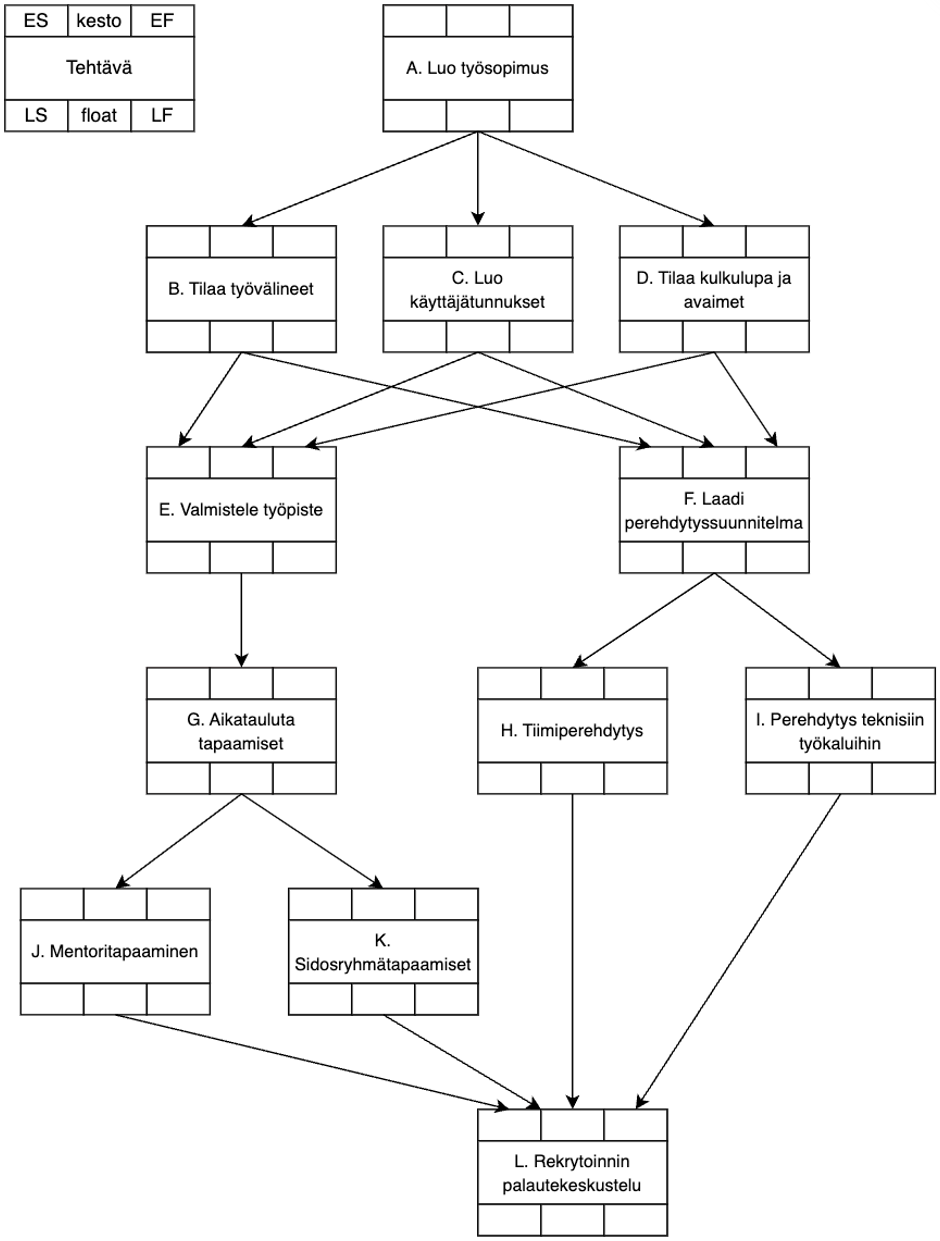
\includegraphics[keepaspectratio]{kuviot/cpm.png}}

}

\caption{\label{fig-cpm-teht}Työntekijän rekrytoinnin prosessi
projektiverkkona kriittisen polun laskentaa varten}

\end{figure}%

\section{Tehtävä 13}\label{tehtuxe4vuxe4-13}

Keksi muutama hyödyllinen prosessien hallintaa tai analysointia tukeva
näkymä, jotka voitaisiin rakentaa kokonaisarkkitehtuuri-informaation
perusteella. Näkymät voivat olla esimerkiksi lämpökartta- tai
liikennevalotyylisiä, kojetaulutyyppisiä mittaristoja, numeerisia
yhteenvetoja, eri arkkitehtuurinäkökulmia yhdistäviä graafisia malleja
tai muita vastaavia.

\section{Tehtävä 14}\label{tehtuxe4vuxe4-14}

Anna tehtävän 3 haastattelutranskriptio jollekin kielimallille ja pyydä
sitä tunnistamaan prosessin vaiheet, roolit, päätöskohdat sekä virhe- ja
poikkeustilanteet. Vertaa tulosta omaan ratkaisuusi. Mitä kielimalli
tunnisti oikein, mitä se jätti huomiotta ja mitä se keksi, vaikka sitä
ei aineistossa ollut? Jos mahdollista, tee sama kahdella eri
kielimallilla ja vertaa niiden tuloksia keskenään.

\section{Tehtävä 15}\label{tehtuxe4vuxe4-15}

Anna jokin tekemäsi monimutkaisempi BPMN-malli kielimallille joko kuvana
tai .bpmn-tiedostona (BPMN XML) ja pyydä sitä arvioimaan mallin
oikeellisuutta ja ymmärrettävyyttä Mendlingin ym. (2010) seitsemän
mallinnusohjeen (7PMG) valossa. Tarkista arvio itse: mitkä kielimallin
huomioista pitivät paikkansa ja mitkä olivat virheellisiä? Kuinka paljon
työtä arvion tarkistaminen vaati verrattuna siihen, että olisit
arvioinut mallin itse? Jos mahdollista, tee sama kahdella eri
kielimallilla ja vertaa tuloksia.

\section{Tehtävä 16 (essee)}\label{tehtuxe4vuxe4-16-essee}

Organisaation toimintaa voidaan tarkastella esimerkiksi funktioina
(osastot ja yksiköt), projekteina tai prosesseina. Valitse jokin
tuntemasi organisaatio, esimerkiksi oma työpaikkasi, oppilaitoksesi tai
harrastusseurasi, ja pohdi, mitä etuja ja haittoja sen toiminnan
tarkastelusta prosessien kautta olisi. Mitkä organisaation toiminnoista
ovat luontevimmin prosesseja, mitkä projekteja ja mitkä funktioita? Mitä
muuttuisi, jos organisaatioon nimettäisiin prosessinomistajat?

Laajuus 2--3 sivua. Käytä vähintään kolmea lähdettä, joista ainakin yksi
on kirjan lähdeluettelon ulkopuolelta.

\section{Tehtävä 17 (essee)}\label{tehtuxe4vuxe4-17-essee}

''\emph{You get what you measure.}'' Kirjoita essee prosessimittareiden
haitallisista sivuvaikutuksista. Kuvaa vähintään kaksi esimerkkiä,
joissa mittari ohjaa toimintaa ei-toivottuun suuntaan. Esimerkit voivat
olla omasta kokemuksestasi, uutisista tai tutkimuskirjallisuudesta.
Selvitä, mitä tarkoittaa Goodhartin laki, ja pohdi, miten mittaristo
voidaan suunnitella niin, että sen `väärinkäyttö' on mahdollisimman
vaikeaa.

Laajuus 2--3 sivua.

\section{Tehtävä 18 (essee)}\label{tehtuxe4vuxe4-18-essee}

Vertaa prosessien jatkuvaa parantamista (BPI, PDCA, kaizen) ja
radikaalia uudistamista (BPR). Millaisissa tilanteissa toinen
lähestymistapa on toista parempi? Pohdi erityisesti
toiminnanohjausjärjestelmän (ERP) käyttöönottoa: onko se luonteeltaan
jatkuvaa parantamista, radikaalia uudistamista vai jotain muuta? Kumpaa
tulisi muuttaa, prosesseja vai järjestelmää, kun ne eivät sovi yhteen?

Laajuus 2--3 sivua.

\section{Tehtävä 19 (essee)}\label{tehtuxe4vuxe4-19-essee}

Valitse jokin organisaation tukiprosessi, esimerkiksi palkanlaskenta,
IT-tuki, siivous tai rekrytointi. Arvioi luvussa 4 esitellyn McIvorin
viitekehyksen avulla, kannattaisiko prosessi ulkoistaa. Käsittele
ainakin seuraavia näkökulmia: prosessin kriittisyys ja kytkökset
ydinprosesseihin, kustannukset, osaaminen ja sen säilyminen, tietosuoja
sekä palvelun takaisinoton (insourcing) mahdollisuus.

Laajuus 2--3 sivua.

\section{Tehtävä 20 (essee)}\label{tehtuxe4vuxe4-20-essee}

BPMN-mallit kuvaavat prosessin työnkulun tarkasti, mutta eivät juurikaan
kerro, mihin prosessi liittyy organisaation kokonaisuudessa. Pohdi
kokonaisarkkitehtuurin ja ArchiMaten roolia prosessien hallinnassa.
Millaisiin kysymyksiin arkkitehtuurimallit vastaavat paremmin kuin
prosessimallit, ja päinvastoin? Kenen organisaatiossa pitäisi vastata
siitä, että prosessimallit ja arkkitehtuurikuvaukset pysyvät keskenään
yhdenmukaisina?

Laajuus 2--3 sivua.

\section{Tehtävä 21 (essee)}\label{tehtuxe4vuxe4-21-essee}

Ohjelmistorobotiikka (RPA) automatisoi tarkasti määriteltyjä
työnkulkuja, kun taas tekoälyagentit voivat päättää itse, mitä tehtäviä
ne suorittavat ja missä järjestyksessä. Pohdi, millaisiin prosesseihin
kumpikin soveltuu. Missä kohdissa prosessia ihmisen tulisi olla mukana
päätöksenteossa (\emph{human in the loop})? Kuka vastaa virheestä, jonka
agentti tekee?

Laajuus 2-3 sivua.

\section{BPMN-mallinnustehtäviä}\label{bpmn-mallinnustehtuxe4viuxe4}

Tämän osion tehtävät keskittyvät BPMN-mallintamiseen. Ne on ryhmitelty
aiheittain, ja kunkin aiheen sisällä lyhyet harjoitukset ovat ensin.
Lyhyissä tehtävissä keskitytään yhteen tai muutamaan BPMN-kielen
piirteeseen, ja yhden tehtävän tekemiseen kuluu tyypillisesti 5--15
minuuttia. Laajemmiksi merkityt tehtävät vaativat enemmän aikaa ja
yhdistelevät useampia piirteitä. Mallit voi piirtää paperille, Camunda
Modelerilla tai Draw.io:lla, ja Token Simulationilla voit testata,
toimiiko mallisi niin kuin olit ajatellut.

Jokaisen tehtävän perässä on sanallinen malliratkaisu. Yritä ratkaista
tehtävä ensin itse. Huomaa, että useimpiin tehtäviin on useampia oikeita
ratkaisuja.

\subsection{Tehtävät, tapahtumat ja
järjestysvirrat}\label{tehtuxe4vuxe4t-tapahtumat-ja-juxe4rjestysvirrat}

\subsubsection{BPMN-tehtävä 1}\label{bpmn-tehtuxe4vuxe4-1}

Mallinna aamukahvin keittäminen. Prosessiin kuuluvat tehtävät
\emph{Keitä kahvi}, \emph{Kaada kahvi kuppiin} ja \emph{Juo kahvi}.
Käytä yhtä aloitus- ja yhtä lopetustapahtumaa.

\begin{tcolorbox}[enhanced jigsaw, arc=.35mm, bottomrule=.15mm, bottomtitle=1mm, breakable, colback=white, colbacktitle=quarto-callout-tip-color!10!white, colframe=quarto-callout-tip-color-frame, coltitle=black, left=2mm, leftrule=.75mm, opacityback=0, opacitybacktitle=0.6, rightrule=.15mm, title=\textcolor{quarto-callout-tip-color}{\faLightbulb}\hspace{0.5em}{Malliratkaisu}, titlerule=0mm, toprule=.15mm, toptitle=1mm]

Start Event → \emph{Keitä kahvi} → \emph{Kaada kahvi kuppiin} →
\emph{Juo kahvi} → End Event. Elementit yhdistetään järjestysvirroilla.
Tapahtumat kannattaa nimetä tilaa kuvaavasti, esimerkiksi
''Kahvihammasta kolottaa'' ja ''Kahvi juotu''.

\end{tcolorbox}

\subsubsection{BPMN-tehtävä 2}\label{bpmn-tehtuxe4vuxe4-2}

Nimeä seuraavat tehtävät uudelleen verbi-objekti-muotoon: \emph{Laskun
hyväksyntä}, \emph{Tilausten käsittely ja lähettäminen},
\emph{Sähköposti} ja \emph{Asiakas}. Mitä ongelmia nimeämisessä huomaat?

\begin{tcolorbox}[enhanced jigsaw, arc=.35mm, bottomrule=.15mm, bottomtitle=1mm, breakable, colback=white, colbacktitle=quarto-callout-tip-color!10!white, colframe=quarto-callout-tip-color-frame, coltitle=black, left=2mm, leftrule=.75mm, opacityback=0, opacitybacktitle=0.6, rightrule=.15mm, title=\textcolor{quarto-callout-tip-color}{\faLightbulb}\hspace{0.5em}{Malliratkaisu}, titlerule=0mm, toprule=.15mm, toptitle=1mm]

\begin{itemize}
\tightlist
\item
  \emph{Laskun hyväksyntä} → \emph{Hyväksy lasku}
\item
  \emph{Tilausten käsittely ja lähettäminen} → kaksi tehtävää:
  \emph{Käsittele tilaus} ja \emph{Lähetä tilaus}. Yksi tehtävä kuvaa
  yhtä toimintoa, ja yksikkömuoto sopii paremmin, koska yksi
  prosessi-instanssi käsittelee yhden tilauksen.
\item
  \emph{Sähköposti} ja \emph{Asiakas} eivät kerro, mitä tehdään. Ilman
  asiayhteyttä niitä ei voi nimetä uudelleen. Vaihtoehtoja ovat
  esimerkiksi \emph{Lähetä vahvistussähköposti} ja \emph{Rekisteröi
  asiakas}.
\end{itemize}

\end{tcolorbox}

\subsubsection{BPMN-tehtävä 3}\label{bpmn-tehtuxe4vuxe4-3}

Kirjaston lainaustiskillä asiakas valitsee kirjan ja esittää
kirjastokorttinsa. Kirjastonhoitaja kirjaa lainan ja antaa asiakkaalle
kuitin. Mallinna prosessi yhtenä uima-altaana (\emph{Kirjasto}), jossa
on kaksi uimarataa (\emph{Asiakas} ja \emph{Kirjastonhoitaja}).

\begin{tcolorbox}[enhanced jigsaw, arc=.35mm, bottomrule=.15mm, bottomtitle=1mm, breakable, colback=white, colbacktitle=quarto-callout-tip-color!10!white, colframe=quarto-callout-tip-color-frame, coltitle=black, left=2mm, leftrule=.75mm, opacityback=0, opacitybacktitle=0.6, rightrule=.15mm, title=\textcolor{quarto-callout-tip-color}{\faLightbulb}\hspace{0.5em}{Malliratkaisu}, titlerule=0mm, toprule=.15mm, toptitle=1mm]

Asiakkaan radalla: Start Event → \emph{Valitse kirja} → \emph{Esitä
kirjastokortti}. Järjestysvirta jatkuu kirjastonhoitajan radalle:
\emph{Kirjaa laina} → \emph{Anna kuitti} → End Event. Saman altaan
ratojen välillä käytetään järjestysvirtaa, ei viestivirtaa.

\end{tcolorbox}

\subsubsection{BPMN-tehtävä 4}\label{bpmn-tehtuxe4vuxe4-4}

Valitse kullekin tehtävälle sopivin BPMN-tehtävätyyppi (User, Manual,
Service, Script, Business Rule, Send tai Receive Task):

\begin{enumerate}
\def\labelenumi{\arabic{enumi}.}
\tightlist
\item
  Kanna paketti autoon.
\item
  Hyväksy matkalasku matkahallintajärjestelmässä.
\item
  Hae yrityksen tiedot YTJ:n rajapinnasta.
\item
  Laske tilauksen arvonlisävero.
\item
  Päätä lainan myöntämisestä luottopolitiikan sääntöjen perusteella.
\item
  Lähetä asiakkaalle tilausvahvistus.
\item
  Odota toimittajan tarjousta.
\end{enumerate}

\begin{tcolorbox}[enhanced jigsaw, arc=.35mm, bottomrule=.15mm, bottomtitle=1mm, breakable, colback=white, colbacktitle=quarto-callout-tip-color!10!white, colframe=quarto-callout-tip-color-frame, coltitle=black, left=2mm, leftrule=.75mm, opacityback=0, opacitybacktitle=0.6, rightrule=.15mm, title=\textcolor{quarto-callout-tip-color}{\faLightbulb}\hspace{0.5em}{Malliratkaisu}, titlerule=0mm, toprule=.15mm, toptitle=1mm]

\begin{enumerate}
\def\labelenumi{\arabic{enumi}.}
\tightlist
\item
  Manual Task
\item
  User Task
\item
  Service Task
\item
  Script Task
\item
  Business Rule Task
\item
  Send Task (myös Service Task on mahdollinen, jos lähetys tehdään
  sähköpostipalvelun kautta)
\item
  Receive Task (tai Message Intermediate Catch Event)
\end{enumerate}

\end{tcolorbox}

\subsubsection{BPMN-tehtävä 5}\label{bpmn-tehtuxe4vuxe4-5}

Laadi looginen prosessimalli ostoksilla käynnistä. Käytä mallissa viittä
perusmuotoista tehtäväelementtiä ja nimeä tehtävät
verbi-objekti-muotoon.

\begin{tcolorbox}[enhanced jigsaw, arc=.35mm, bottomrule=.15mm, bottomtitle=1mm, breakable, colback=white, colbacktitle=quarto-callout-tip-color!10!white, colframe=quarto-callout-tip-color-frame, coltitle=black, left=2mm, leftrule=.75mm, opacityback=0, opacitybacktitle=0.6, rightrule=.15mm, title=\textcolor{quarto-callout-tip-color}{\faLightbulb}\hspace{0.5em}{Malliratkaisu}, titlerule=0mm, toprule=.15mm, toptitle=1mm]

Esimerkiksi: Start Event ''Ruokakaappi tyhjä'' → \emph{Laadi ostoslista}
→ \emph{Mene kauppaan} → \emph{Kerää tuotteet koriin} → \emph{Maksa
ostokset} → \emph{Kanna ostokset kotiin} → End Event ''Ostokset tehty''.
Kaikki tehtävät ovat yleisiä tehtäväelementtejä ilman tyyppimerkintää,
ja ne on nimetty käskymuotoisella verbillä ja objektilla. Tehtävien
rajaus voi vaihdella: olennaista on, että jokainen tehtävä kuvaa yhtä
selvästi erottuvaa toimintoa ja että mallissa on yksi aloitus- ja yksi
lopetustapahtuma.

\end{tcolorbox}

\subsubsection{BPMN-tehtävä 6}\label{bpmn-tehtuxe4vuxe4-6}

Laadi valitsemastasi aiheesta looginen prosessimalli, jossa käytät
seuraavia tehtävätyyppejä tässä järjestyksessä: Manual Task, User Task,
Manual Task, User Task, Manual Task.

\begin{tcolorbox}[enhanced jigsaw, arc=.35mm, bottomrule=.15mm, bottomtitle=1mm, breakable, colback=white, colbacktitle=quarto-callout-tip-color!10!white, colframe=quarto-callout-tip-color-frame, coltitle=black, left=2mm, leftrule=.75mm, opacityback=0, opacitybacktitle=0.6, rightrule=.15mm, title=\textcolor{quarto-callout-tip-color}{\faLightbulb}\hspace{0.5em}{Malliratkaisu}, titlerule=0mm, toprule=.15mm, toptitle=1mm]

Esimerkiksi paketin lähettäminen pakettiautomaatista: Manual Task
\emph{Pakkaa tuote laatikkoon} → User Task \emph{Osta lähetystunnus
verkkopalvelusta} → Manual Task \emph{Kiinnitä osoitekortti pakettiin} →
User Task \emph{Avaa automaatin luukku mobiilisovelluksella} → Manual
Task \emph{Aseta paketti luukkuun}. Manual Task tehdään kokonaan ilman
tietojärjestelmää. User Task on ihmisen tekemä tehtävä, jossa käytetään
tietojärjestelmää. Hyvä tarkistuskysymys on, voisiko tehtävän tehdä myös
sähkökatkon aikana.

\end{tcolorbox}

\subsubsection{BPMN-tehtävä 7}\label{bpmn-tehtuxe4vuxe4-7}

Piirrä seuraava tapahtumasarja prosessiksi ja käytä mallissa sopivissa
kohdissa Service Task-, Script Task- ja Business Rule Task -tehtäviä.

\begin{enumerate}
\def\labelenumi{\arabic{enumi}.}
\tightlist
\item
  Vastaanota tilaus.
\item
  Arvioi kampanja-alennus.
\item
  Tarkista maksu ulkoisesta maksupalvelusta.
\item
  Päivitä varastosaldot ERP-järjestelmään.
\item
  Muodosta pakkauslistat tilauksen riveistä.
\item
  Tilaa nouto kuljetusliikkeeltä.
\item
  Lähetä tilausvahvistus asiakkaalle.
\item
  Päätä prosessi.
\end{enumerate}

\begin{tcolorbox}[enhanced jigsaw, arc=.35mm, bottomrule=.15mm, bottomtitle=1mm, breakable, colback=white, colbacktitle=quarto-callout-tip-color!10!white, colframe=quarto-callout-tip-color-frame, coltitle=black, left=2mm, leftrule=.75mm, opacityback=0, opacitybacktitle=0.6, rightrule=.15mm, title=\textcolor{quarto-callout-tip-color}{\faLightbulb}\hspace{0.5em}{Malliratkaisu}, titlerule=0mm, toprule=.15mm, toptitle=1mm]

Message Start Event ''Tilaus vastaanotettu'' (kohta 1) → Business Rule
Task \emph{Arvioi kampanja-alennus} (2) → Service Task \emph{Tarkista
maksu} (3) → Service Task \emph{Päivitä varastosaldot} (4) → Script Task
\emph{Muodosta pakkauslistat} (5) → Service Task \emph{Tilaa nouto
kuljetusliikkeeltä} (6) → Send Task \emph{Lähetä tilausvahvistus} (7) →
End Event (8).

Perustelut: alennuksen arviointi on sääntöpohjainen päätös
(päätöstaulu). Maksupalvelu, ERP ja kuljetusliikkeen järjestelmä ovat
ulkoisia järjestelmiä, joita kutsutaan rajapinnan kautta.
Pakkauslistojen muodostaminen tilausriveistä on prosessin sisäistä
tiedonkäsittelyä, joka sopii skriptille. Kohdan 7 voi esittää myös
Service Taskina, jos vahvistus lähetetään sähköpostipalvelun kautta.
Tarkempi malli lisäisi maksun tarkistuksen jälkeen portin, jossa
käsitellään epäonnistunut maksu. Kohdat 4 ja 5 voisi myös suorittaa
rinnakkain.

\end{tcolorbox}

\subsection{Portit}\label{portit-1}

\subsubsection{BPMN-tehtävä 8}\label{bpmn-tehtuxe4vuxe4-8}

Ennen ulos lähtemistä tarkistetaan sääennuste. Jos sataa, otetaan mukaan
sateenvarjo. Lopuksi lähdetään ulos. Mallinna prosessi Exclusive
Gatewayn avulla.

\begin{tcolorbox}[enhanced jigsaw, arc=.35mm, bottomrule=.15mm, bottomtitle=1mm, breakable, colback=white, colbacktitle=quarto-callout-tip-color!10!white, colframe=quarto-callout-tip-color-frame, coltitle=black, left=2mm, leftrule=.75mm, opacityback=0, opacitybacktitle=0.6, rightrule=.15mm, title=\textcolor{quarto-callout-tip-color}{\faLightbulb}\hspace{0.5em}{Malliratkaisu}, titlerule=0mm, toprule=.15mm, toptitle=1mm]

Start Event → \emph{Tarkista sääennuste} → Exclusive Gateway
''Sataako?''. Haara ''Kyllä'' → \emph{Ota sateenvarjo} → yhdistävä
Exclusive Gateway. Haara ''Ei'' johtaa suoraan yhdistävään porttiin.
Portin jälkeen \emph{Lähde ulos} → End Event. Yhdistävä portti on
tarpeen, jotta molemmat haarat päätyvät samaan jatkoon. Ilman sitä
mallissa olisi kaksi rinnakkaista loppua.

\end{tcolorbox}

\subsubsection{BPMN-tehtävä 9}\label{bpmn-tehtuxe4vuxe4-9}

Elokuvateatterin kassalla myydään lippuja K18-elokuvaan. Kassa pyytää
asiakkaalta henkilöllisyystodistuksen. Jos asiakas on täysi-ikäinen,
hänelle myydään lippu, ja muuten myynnistä kieltäydytään. Mallinna
prosessi. Käytätkö yhtä vai kahta lopetustapahtumaa? Perustele
valintasi.

\begin{tcolorbox}[enhanced jigsaw, arc=.35mm, bottomrule=.15mm, bottomtitle=1mm, breakable, colback=white, colbacktitle=quarto-callout-tip-color!10!white, colframe=quarto-callout-tip-color-frame, coltitle=black, left=2mm, leftrule=.75mm, opacityback=0, opacitybacktitle=0.6, rightrule=.15mm, title=\textcolor{quarto-callout-tip-color}{\faLightbulb}\hspace{0.5em}{Malliratkaisu}, titlerule=0mm, toprule=.15mm, toptitle=1mm]

Start Event → \emph{Pyydä henkilöllisyystodistus} → Exclusive Gateway
''Onko asiakas täysi-ikäinen?''. Haara ''Kyllä'' → \emph{Myy lippu},
haara ''Ei'' → \emph{Kieltäydy myymästä}. Molemmat ratkaisut ovat
oikein. Kaksi nimettyä lopetustapahtumaa (''Lippu myyty'' ja ''Myynti
evätty'') tekevät lopputuloksista näkyviä. Yksi lopetustapahtuma
yhdistävän portin jälkeen noudattaa Mendlingin ym. ohjetta yhdestä
aloitus- ja lopetustapahtumasta.

\end{tcolorbox}

\subsubsection{BPMN-tehtävä 10}\label{bpmn-tehtuxe4vuxe4-10}

Postin palvelupisteessä lähetyksen hinnoittelu riippuu painosta. Alle 2
kg:n lähetys hinnoitellaan kirjeenä ja 2--30 kg:n lähetys pakettina.
Kaikki muut lähetykset hinnoitellaan rahtina. Mallinna päätös niin, että
prosessi ei voi jäädä jumiin.

\begin{tcolorbox}[enhanced jigsaw, arc=.35mm, bottomrule=.15mm, bottomtitle=1mm, breakable, colback=white, colbacktitle=quarto-callout-tip-color!10!white, colframe=quarto-callout-tip-color-frame, coltitle=black, left=2mm, leftrule=.75mm, opacityback=0, opacitybacktitle=0.6, rightrule=.15mm, title=\textcolor{quarto-callout-tip-color}{\faLightbulb}\hspace{0.5em}{Malliratkaisu}, titlerule=0mm, toprule=.15mm, toptitle=1mm]

\emph{Punnitse lähetys} → Exclusive Gateway, josta lähtee kolme haaraa.
Ehdolliset virrat ovat \texttt{paino\ \textless{}\ 2} →
\emph{Hinnoittele kirjeenä} ja
\texttt{paino\ \textgreater{}=\ 2\ and\ paino\ \textless{}=\ 30} →
\emph{Hinnoittele pakettina}. Kolmas haara on oletusvirta (Default Flow)
→ \emph{Hinnoittele rahtina}. Oletusvirta takaa, että prosessi etenee,
vaikka mikään ehto ei täyttyisi. Lopuksi haarat yhdistetään Exclusive
Gatewaylla.

\end{tcolorbox}

\subsubsection{BPMN-tehtävä 11}\label{bpmn-tehtuxe4vuxe4-11}

Kun juhlapäivä on päätetty, juhlien järjestäjä lähettää kutsut, tilaa
kakun ja siivoaa kodin. Näillä tehtävillä ei ole keskinäistä
järjestystä. Kun kaikki on tehty, pidetään juhlat. Mallinna prosessi.

\begin{tcolorbox}[enhanced jigsaw, arc=.35mm, bottomrule=.15mm, bottomtitle=1mm, breakable, colback=white, colbacktitle=quarto-callout-tip-color!10!white, colframe=quarto-callout-tip-color-frame, coltitle=black, left=2mm, leftrule=.75mm, opacityback=0, opacitybacktitle=0.6, rightrule=.15mm, title=\textcolor{quarto-callout-tip-color}{\faLightbulb}\hspace{0.5em}{Malliratkaisu}, titlerule=0mm, toprule=.15mm, toptitle=1mm]

\emph{Päätä juhlapäivä} → Parallel Gateway (jakava), josta lähtee kolme
haaraa: \emph{Lähetä kutsut}, \emph{Tilaa kakku} ja \emph{Siivoa koti}.
Haarat yhdistetään Parallel Gatewaylla, joka odottaa kaikkien kolmen
haaran valmistumista. Sen jälkeen \emph{Pidä juhlat} → End Event.

\end{tcolorbox}

\subsubsection{BPMN-tehtävä 12}\label{bpmn-tehtuxe4vuxe4-12}

Hampurilaisravintolassa asiakas voi valita annokseensa lisukkeeksi
ranskalaiset, salaatin ja juoman: yhden, kaksi tai kaikki kolme. Kun
lisukkeet on valmistettu, tarjotin kootaan. Mallinna prosessi.

\begin{tcolorbox}[enhanced jigsaw, arc=.35mm, bottomrule=.15mm, bottomtitle=1mm, breakable, colback=white, colbacktitle=quarto-callout-tip-color!10!white, colframe=quarto-callout-tip-color-frame, coltitle=black, left=2mm, leftrule=.75mm, opacityback=0, opacitybacktitle=0.6, rightrule=.15mm, title=\textcolor{quarto-callout-tip-color}{\faLightbulb}\hspace{0.5em}{Malliratkaisu}, titlerule=0mm, toprule=.15mm, toptitle=1mm]

\emph{Ota tilaus vastaan} → Inclusive Gateway, josta lähtee kolme
ehdollista haaraa: \emph{Paista ranskalaiset}, \emph{Valmista salaatti}
ja \emph{Kaada juoma}. Haarat yhdistetään Inclusive Gatewaylla, joka
odottaa kaikkia aktivoituneita haaroja. Sen jälkeen \emph{Kokoa
tarjotin}. Jos on mahdollista, ettei asiakas valitse yhtään lisuketta,
jakavaan porttiin tarvitaan oletusvirta, joka johtaa suoraan yhdistävään
porttiin.

\end{tcolorbox}

\subsubsection{BPMN-tehtävä 13}\label{bpmn-tehtuxe4vuxe4-13}

Etsi virhe. Mallissa Exclusive Gateway jakaa prosessin kahteen haaraan:
\emph{Lähetä lasku} ja \emph{Lähetä maksumuistutus}. Haarat yhdistetään
Parallel Gatewaylla, jonka jälkeen tulee tehtävä \emph{Kirjaa
tapahtuma}. Mitä prosessia suoritettaessa tapahtuu?

\begin{tcolorbox}[enhanced jigsaw, arc=.35mm, bottomrule=.15mm, bottomtitle=1mm, breakable, colback=white, colbacktitle=quarto-callout-tip-color!10!white, colframe=quarto-callout-tip-color-frame, coltitle=black, left=2mm, leftrule=.75mm, opacityback=0, opacitybacktitle=0.6, rightrule=.15mm, title=\textcolor{quarto-callout-tip-color}{\faLightbulb}\hspace{0.5em}{Malliratkaisu}, titlerule=0mm, toprule=.15mm, toptitle=1mm]

Prosessi jumiutuu. Exclusive Gateway aktivoi vain toisen haaran, mutta
Parallel Gateway odottaa, että molemmat haarat saapuvat. \emph{Kirjaa
tapahtuma} ei siis koskaan käynnisty. Korjaus: haarat yhdistetään
Exclusive Gatewaylla.

\end{tcolorbox}

\subsubsection{BPMN-tehtävä 14}\label{bpmn-tehtuxe4vuxe4-14}

Etsi virhe. Mallissa Parallel Gateway jakaa prosessin kahteen haaraan:
\emph{Varaa hotelli} ja \emph{Varaa lento}. Haarat yhdistetään Exclusive
Gatewaylla, jonka jälkeen tulee tehtävä \emph{Lähetä matkasuunnitelma}.
Mitä tapahtuu?

\begin{tcolorbox}[enhanced jigsaw, arc=.35mm, bottomrule=.15mm, bottomtitle=1mm, breakable, colback=white, colbacktitle=quarto-callout-tip-color!10!white, colframe=quarto-callout-tip-color-frame, coltitle=black, left=2mm, leftrule=.75mm, opacityback=0, opacitybacktitle=0.6, rightrule=.15mm, title=\textcolor{quarto-callout-tip-color}{\faLightbulb}\hspace{0.5em}{Malliratkaisu}, titlerule=0mm, toprule=.15mm, toptitle=1mm]

\emph{Lähetä matkasuunnitelma} suoritetaan kahdesti, koska Exclusive
Gateway päästää jokaisen saapuvan haaran läpi heti odottamatta toista.
Korjaus: haarat yhdistetään Parallel Gatewaylla.

\end{tcolorbox}

\subsubsection{BPMN-tehtävä 15}\label{bpmn-tehtuxe4vuxe4-15}

Opiskelija kirjoittaa esseen ja pyytää siitä palautetta. Jos opettaja ei
hyväksy esseetä, opiskelija korjaa sen ja pyytää palautetta uudelleen.
Hyväksytty essee palautetaan. Mallinna toisto porteilla ilman
Loop-merkintää.

\begin{tcolorbox}[enhanced jigsaw, arc=.35mm, bottomrule=.15mm, bottomtitle=1mm, breakable, colback=white, colbacktitle=quarto-callout-tip-color!10!white, colframe=quarto-callout-tip-color-frame, coltitle=black, left=2mm, leftrule=.75mm, opacityback=0, opacitybacktitle=0.6, rightrule=.15mm, title=\textcolor{quarto-callout-tip-color}{\faLightbulb}\hspace{0.5em}{Malliratkaisu}, titlerule=0mm, toprule=.15mm, toptitle=1mm]

Start Event → \emph{Kirjoita essee} → yhdistävä Exclusive Gateway →
\emph{Pyydä palautetta} → Exclusive Gateway ''Hyväksytty?''. Haara
''Kyllä'' → \emph{Palauta essee} → End Event. Haara ''Ei'' →
\emph{Korjaa essee} → takaisin yhdistävään porttiin ennen tehtävää
\emph{Pyydä palautetta}. Taaksepäin palaava järjestysvirta johdetaan
porttiin eikä suoraan tehtävään, jotta tehtävään saapuu vain yksi virta.

\end{tcolorbox}

\subsubsection{BPMN-tehtävä 16
(laajempi)}\label{bpmn-tehtuxe4vuxe4-16-laajempi}

Piirrä prosessimalli seuraavasta tapauksesta: Prosessi käynnistyy
tuotetilauksen vastaanottamisella. Jos tilattua tuotetta löytyy
valmiina, se toimitetaan asiakkaalle lähetysvahvistuksen saattelemana.
Mikäli tilattua tuotetta ei ole varastossa, tarkastetaan ensin, ovatko
kaikki sen kokoamiseen tarvittavat komponentit yrityksen pajalla.
Tarvittaessa komponentteja tilataan toimittajalta. Mikäli tarvittavia
osia ei ole saatavilla, tilaus perutaan ja siitä ilmoitetaan
asiakkaalle. Kun tuote on saatu valmistettua, se lähetetään asiakkaalle
pikatoimituksena. Lisäksi asiakkaalle lähetetään lähetysvahvistus.

\begin{tcolorbox}[enhanced jigsaw, arc=.35mm, bottomrule=.15mm, bottomtitle=1mm, breakable, colback=white, colbacktitle=quarto-callout-tip-color!10!white, colframe=quarto-callout-tip-color-frame, coltitle=black, left=2mm, leftrule=.75mm, opacityback=0, opacitybacktitle=0.6, rightrule=.15mm, title=\textcolor{quarto-callout-tip-color}{\faLightbulb}\hspace{0.5em}{Malliratkaisu}, titlerule=0mm, toprule=.15mm, toptitle=1mm]

Message Start Event ''Tilaus vastaanotettu'' → \emph{Tarkista
varastosaldo} → Exclusive Gateway ''Tuote varastossa?''.

\begin{itemize}
\tightlist
\item
  Haara ''Kyllä'' → \emph{Toimita tuote}.
\item
  Haara ''Ei'' → \emph{Tarkista komponentit pajalla} → Exclusive Gateway
  ''Komponentit pajalla?''. Haara ''Kyllä'' vie yhdistävään porttiin.
  Haara ''Ei'' → \emph{Tilaa komponentit toimittajalta} → Exclusive
  Gateway ''Osat saatavilla?'': ''Kyllä'' vie samaan yhdistävään
  porttiin, ''Ei'' → \emph{Peru tilaus} → \emph{Ilmoita asiakkaalle
  peruutuksesta} → End Event ''Tilaus peruttu''. Yhdistävän portin
  jälkeen \emph{Kokoa tuote} → \emph{Lähetä tuote pikatoimituksena}.
\end{itemize}

Molemmat toimitushaarat (\emph{Toimita tuote} ja \emph{Lähetä tuote
pikatoimituksena}) yhdistetään Exclusive Gatewaylla, jonka jälkeen
\emph{Lähetä lähetysvahvistus} → End Event ''Tilaus toimitettu''. Näin
vahvistuksen lähettäminen mallinnetaan vain kerran. Komponenttien
tilaaminen voidaan tarkentaa Send Taskiksi ja toimittajan vastauksen
vastaanotoksi (Receive Task).

\end{tcolorbox}

\subsubsection{BPMN-tehtävä 17}\label{bpmn-tehtuxe4vuxe4-17}

Missä kohdissa seuraavassa prosessimallissa käyttäisit Parallel
Gateway-, Inclusive Gateway- ja Exclusive Gateway -portteja?

\begin{figure}

\centering{

\pandocbounded{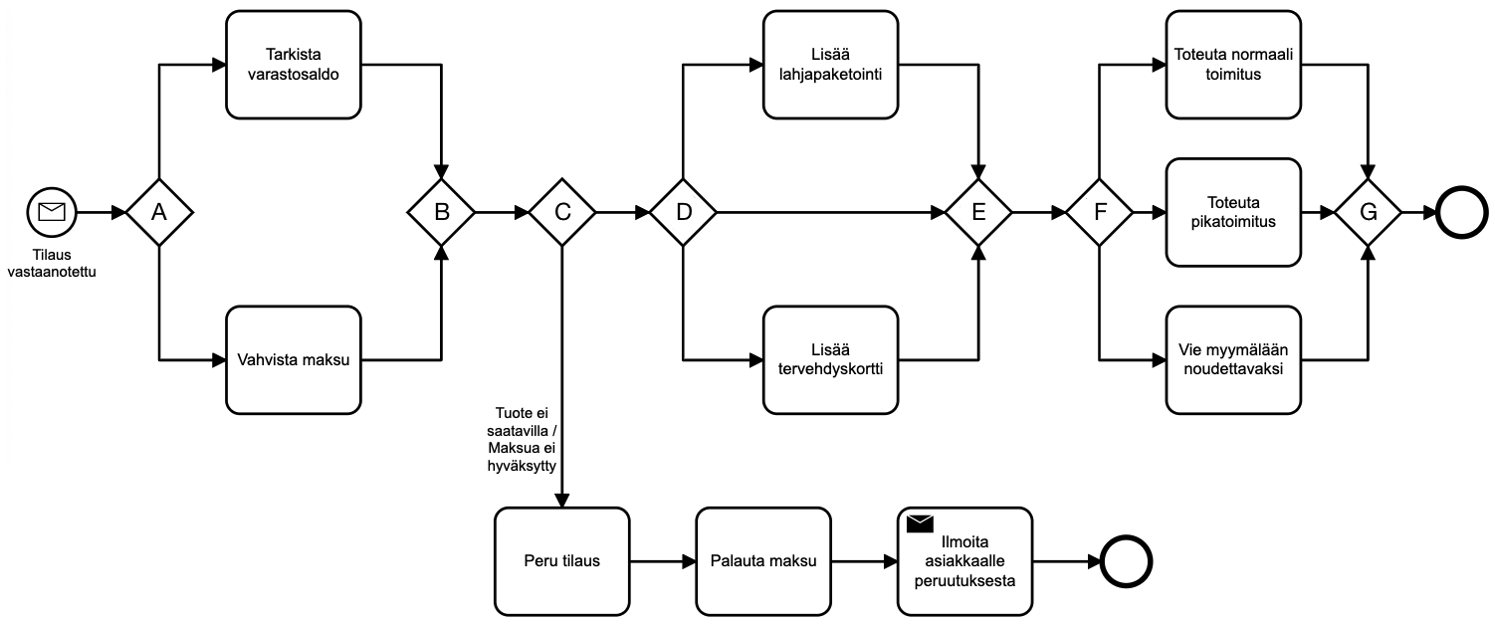
\includegraphics[keepaspectratio]{kuviot/porttitehtava.png}}

}

\caption{\label{fig-porttitehtava}Prosessimalli ilman portteja}

\end{figure}%

\begin{tcolorbox}[enhanced jigsaw, arc=.35mm, bottomrule=.15mm, bottomtitle=1mm, breakable, colback=white, colbacktitle=quarto-callout-tip-color!10!white, colframe=quarto-callout-tip-color-frame, coltitle=black, left=2mm, leftrule=.75mm, opacityback=0, opacitybacktitle=0.6, rightrule=.15mm, title=\textcolor{quarto-callout-tip-color}{\faLightbulb}\hspace{0.5em}{Malliratkaisu}, titlerule=0mm, toprule=.15mm, toptitle=1mm]

\begin{itemize}
\tightlist
\item
  \textbf{A}: Parallel Gateway. Varastosaldo tarkistetaan ja maksu
  vahvistetaan aina, eikä niillä ole keskinäistä järjestystä.
\item
  \textbf{B}: Parallel Gateway, joka odottaa molempien tarkistusten
  valmistumista.
\item
  \textbf{C}: Exclusive Gateway. Joko tilaus voidaan toteuttaa tai se
  perutaan.
\item
  \textbf{D}: Inclusive Gateway. Asiakas voi valita lahjapaketoinnin,
  tervehdyskortin, molemmat tai ei kumpaakaan. Keskimmäinen suora virta
  on oletusvirta, jota käytetään, kun mitään lisäpalvelua ei ole
  valittu.
\item
  \textbf{E}: Inclusive Gateway, joka odottaa kaikkia aktivoituneita
  haaroja.
\item
  \textbf{F}: Exclusive Gateway. Toimitustapoja on kolme, mutta tilaus
  toimitetaan vain yhdellä niistä.
\item
  \textbf{G}: Exclusive Gateway.
\end{itemize}

Huomio mallista: peruutushaarassa maksu palautetaan aina, myös silloin,
kun peruutuksen syynä oli hylätty maksu. Tarkempi malli erottaisi
peruutuksen syyt ja palauttaisi maksun vain, jos se on veloitettu.

\end{tcolorbox}

\subsubsection{BPMN-tehtävä 18}\label{bpmn-tehtuxe4vuxe4-18}

Muuta seuraavaa tilauskäsittelyprosessia niin, että kanta-asiakkaat
saavat tilauksistaan 10 \% alennuksen.

\begin{figure}

\centering{

\pandocbounded{\includegraphics[keepaspectratio]{index_files/mediabag/kuviot/tilauksen-kasittely-valiyhtveto.pdf}}

}

\caption{\label{fig-tilauskäsittely}Tilauksen käsittely}

\end{figure}%

\begin{tcolorbox}[enhanced jigsaw, arc=.35mm, bottomrule=.15mm, bottomtitle=1mm, breakable, colback=white, colbacktitle=quarto-callout-tip-color!10!white, colframe=quarto-callout-tip-color-frame, coltitle=black, left=2mm, leftrule=.75mm, opacityback=0, opacitybacktitle=0.6, rightrule=.15mm, title=\textcolor{quarto-callout-tip-color}{\faLightbulb}\hspace{0.5em}{Malliratkaisu}, titlerule=0mm, toprule=.15mm, toptitle=1mm]

Lisätään tilausjärjestelmän radalle tehtävän \emph{Laske tilauksen
hinta} jälkeen Exclusive Gateway ''Kanta-asiakas?''. Haara ''Kyllä'' →
Script Task \emph{Vähennä 10 \%:n kanta-asiakasalennus} → yhdistävä
Exclusive Gateway. Haara ''Ei'' johtaa suoraan yhdistävään porttiin,
josta prosessi jatkuu tehtävään \emph{Hyväksy tilaus}. Tieto
asiakkuudesta voidaan hakea asiakasrekisteristä (Data Store ja Data
Input Association) tai erillisellä Service Taskilla \emph{Hae
asiakkuustiedot CRM:stä}.

Vaihtoehtoja: alennuksen voi laskea myös osana tehtävää \emph{Laske
tilauksen hinta}, jolloin malli ei muutu lainkaan, mutta alennussääntö
ei näy mallissa. Jos alennussääntöjä on useita, ne kannattaa koota
päätöstauluun ja käyttää Business Rule Taskia \emph{Määritä alennus}.

\end{tcolorbox}

\subsubsection{BPMN-tehtävä 19}\label{bpmn-tehtuxe4vuxe4-19}

Kuvan kuva~\ref{fig-dmn-hakemus-teht} prosessissa \emph{Päätä
hakemuksesta} -Business Rule Task tekee päätöksen kuvan
kuva~\ref{fig-dmn-paatostaulu-teht} päätöstaulun perusteella. Mallinna
sama päätöslogiikka porttien avulla ilman Business Rule Taskia. Kumpi
toteutus on helpompi ylläpitää, jos päätökseen lisätään myöhemmin uusia
ehtoja, esimerkiksi hakijan asuinkunta ja tulot? Miksi?

\begin{figure}

\centering{

\pandocbounded{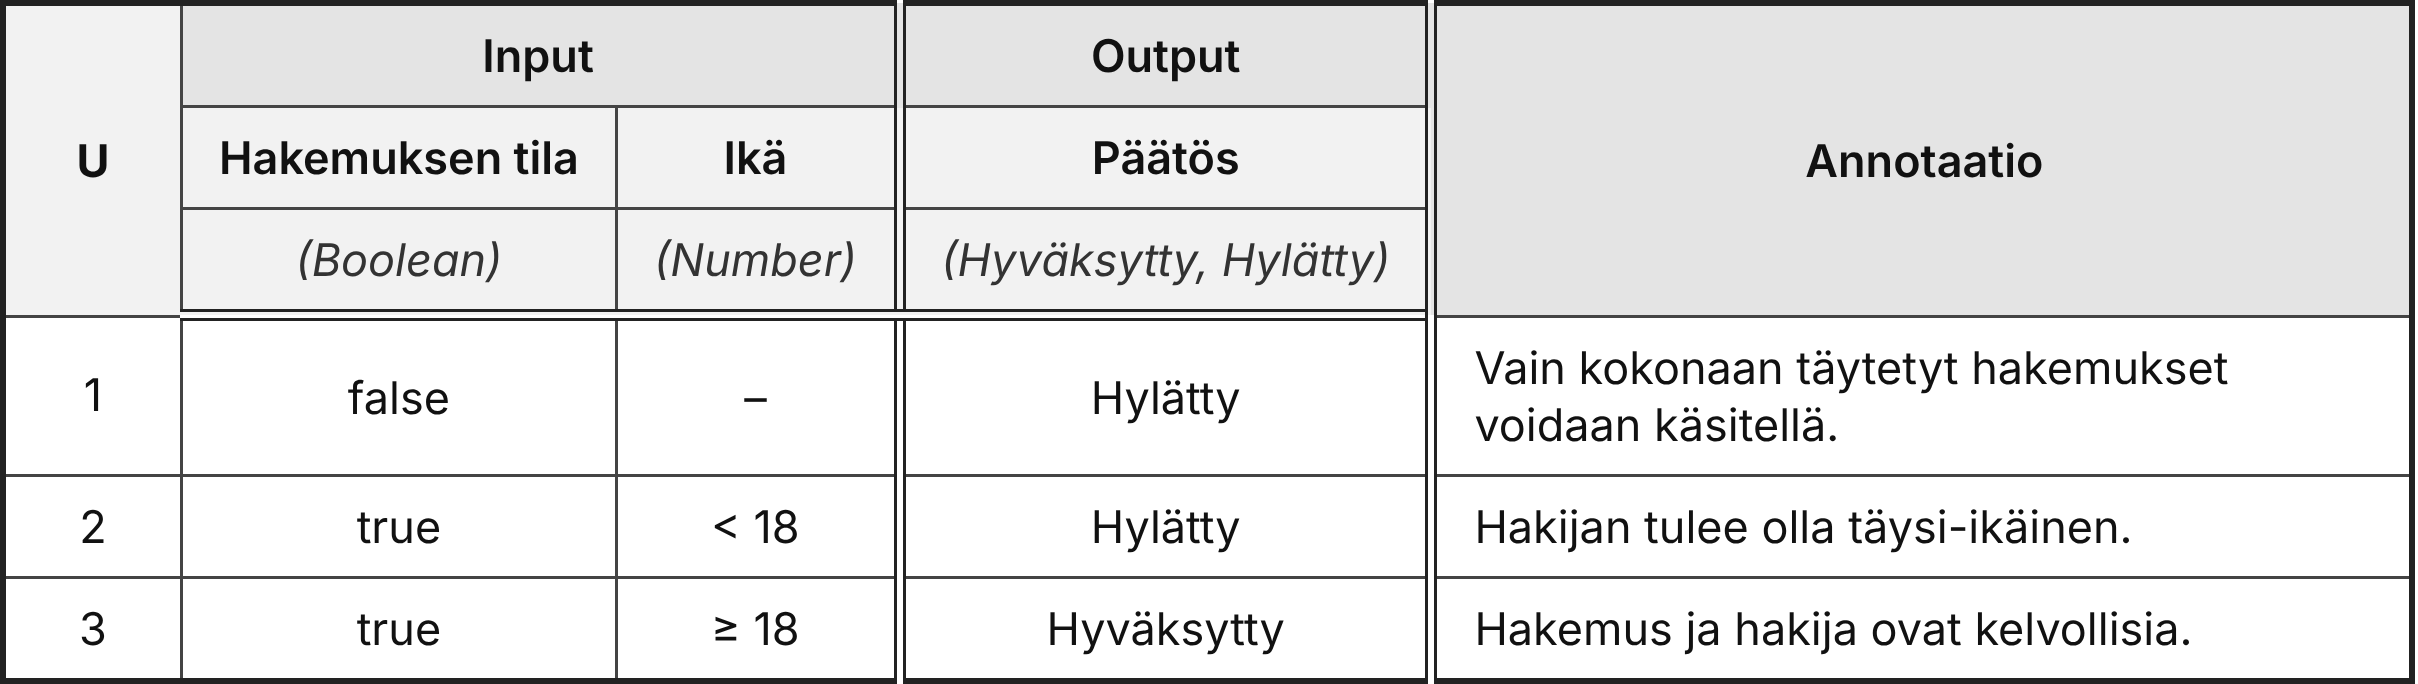
\includegraphics[keepaspectratio]{kuviot/dmn-hakemus.png}}

}

\caption{\label{fig-dmn-hakemus-teht}Hakemuksen käsittely Business Rule
Taskin avulla}

\end{figure}%

\begin{figure}

\centering{

\pandocbounded{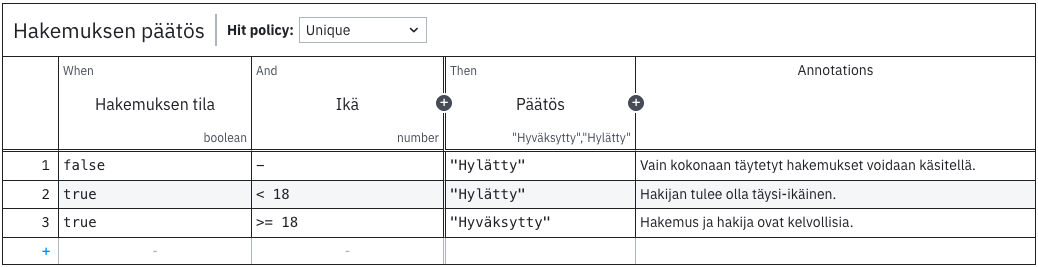
\includegraphics[keepaspectratio]{kuviot/dmn-paatostaulu.png}}

}

\caption{\label{fig-dmn-paatostaulu-teht}Päätöstaulu hakemuksesta
päättämiseksi}

\end{figure}%

\begin{tcolorbox}[enhanced jigsaw, arc=.35mm, bottomrule=.15mm, bottomtitle=1mm, breakable, colback=white, colbacktitle=quarto-callout-tip-color!10!white, colframe=quarto-callout-tip-color-frame, coltitle=black, left=2mm, leftrule=.75mm, opacityback=0, opacitybacktitle=0.6, rightrule=.15mm, title=\textcolor{quarto-callout-tip-color}{\faLightbulb}\hspace{0.5em}{Malliratkaisu}, titlerule=0mm, toprule=.15mm, toptitle=1mm]

Start Event ''Hakemus vastaanotettu'' → Exclusive Gateway ''Hakemus
täytetty kokonaan?''. Haara ''Ei'' → End Event ''Hakemus hylätty''.
Haara ''Kyllä'' → Exclusive Gateway ''Hakija täysi-ikäinen?'': ehto
\texttt{ikä\ \textgreater{}=\ 18} → End Event ''Hakemus hyväksytty'',
ehto \texttt{ikä\ \textless{}\ 18} → End Event ''Hakemus hylätty''.
Vaihtoehtoisesti yksi Exclusive Gateway, jossa on kolme haaraa
päätöstaulun kolmen rivin mukaisesti.

Näin pienen päätöstaulun voi esittää porteilla helposti. Kun ehtoja ja
niiden yhdistelmiä lisätään, porttien määrä kasvaa nopeasti ja malli
muuttuu vaikealukuiseksi. Lisäksi jokainen sääntömuutos edellyttää
prosessimallin muuttamista. Päätöstaulussa liiketoimintasäännöt pysyvät
erillään prosessikulusta. Uuden rivin tai sarakkeen voi lisätä
koskematta prosessiin, ja Unique-hit policy takaa, että täsmälleen yksi
sääntö täyttyy. Porteilla saman joutuu varmistamaan itse muotoilemalla
ehdot toisensa poissulkeviksi ja kattaviksi, esimerkiksi oletusvirran
avulla.

\end{tcolorbox}

\subsubsection{BPMN-tehtävä 20
(laajempi)}\label{bpmn-tehtuxe4vuxe4-20-laajempi}

Piirrä prosessimalli vuoden 2025 itsenäisyyspäivän linnanjuhlistakin
tuttujen lappeenrantalaisten herkkujen, Vetyn ja Atomin, valmistuksesta.
Tee ensin Vetylle ja Atomille omat prosessimallinsa. Tämän jälkeen
yhdistä ne yhdeksi prosessimalliksi, jolla onnistuu molempien
piirakoiden valmistaminen.

Lihapiirakka leikataan auki taskuksi ja väliin lisätään nokare voita.
Piirakkaa lämmitetään höyrykattilassa, kunnes voi sulaa. Höyrytyksen
aikana kuoritaan ja viipaloidaan kovaksi keitetty (13 min.) kananmuna.
Seuraavaksi lisätään piirakan väliin täytteet tilauksen mukaisesti.
Vety-piirakkaan tulee viipaloitu kananmuna sekä neljä viipaletta
savukinkkua. Atomiin asiakas voi valita joko kananmunan tai kinkun.
Lisukkeiksi molempiin on valittavissa kurkkusalaatti, ketsuppi ja
sinappi. Mikäli piirakka syödään heti, se kääräistään voipaperiin. Jos
piirakka on tarkoitus ottaa mukaan, se pakataan lisäksi pahvirasiaan.

\begin{tcolorbox}[enhanced jigsaw, arc=.35mm, bottomrule=.15mm, bottomtitle=1mm, breakable, colback=white, colbacktitle=quarto-callout-tip-color!10!white, colframe=quarto-callout-tip-color-frame, coltitle=black, left=2mm, leftrule=.75mm, opacityback=0, opacitybacktitle=0.6, rightrule=.15mm, title=\textcolor{quarto-callout-tip-color}{\faLightbulb}\hspace{0.5em}{Malliratkaisu}, titlerule=0mm, toprule=.15mm, toptitle=1mm]

\textbf{Vety}: Start Event ''Tilaus vastaanotettu'' → \emph{Leikkaa
piirakka auki} → \emph{Lisää voinokare} → Parallel Gateway → kaksi
haaraa: \emph{Lämmitä piirakkaa höyrykattilassa} ja \emph{Kuori ja
viipaloi kananmuna} → Parallel Gateway → \emph{Lisää kananmunaviipaleet}
→ \emph{Lisää neljä viipaletta savukinkkua} → lisukkeet (ks. alla) →
\emph{Kääri piirakka voipaperiin} → Exclusive Gateway ''Mukaan?'':
''Kyllä'' → \emph{Pakkaa pahvirasiaan} → yhdistävä Exclusive Gateway;
''Ei'' → suoraan yhdistävään porttiin → End Event ''Piirakka valmis''.

Lisukkeet mallinnetaan Inclusive Gatewaylla, josta lähtevät haarat
\emph{Lisää kurkkusalaattia}, \emph{Lisää ketsuppia} ja \emph{Lisää
sinappia} sekä oletusvirta suoraan yhdistävään Inclusive Gatewayhin
siltä varalta, ettei lisukkeita haluta.

\textbf{Atomi}: Muuten sama, mutta voin lisäämisen jälkeen Exclusive
Gateway ''Täyte?''. Kananmunahaarassa piirakan höyrytys sekä kananmunan
kuorinta ja viipalointi tehdään rinnakkain, minkä jälkeen lisätään
kananmuna. Kinkkuhaarassa piirakka höyrytetään ja siihen lisätään
kinkku. Haarat yhdistetään Exclusive Gatewaylla ennen lisukkeita.

\textbf{Yhdistetty malli}: \emph{Leikkaa piirakka auki} → \emph{Lisää
voinokare} → Parallel Gateway → (1) \emph{Lämmitä piirakkaa
höyrykattilassa} ja (2) Exclusive Gateway ''Tarvitaanko kananmunaa?'' →
\emph{Kuori ja viipaloi kananmuna} tai oletusvirta ohi → Parallel
Gateway. Täytteet lisätään Inclusive Gatewaylla: ehto
\texttt{piirakka\ =\ Vety\ tai\ täyte\ =\ kananmuna} → \emph{Lisää
kananmunaviipaleet}, ehto
\texttt{piirakka\ =\ Vety\ tai\ täyte\ =\ kinkku} → \emph{Lisää
savukinkku}. Vedyssä molemmat haarat aktivoituvat, Atomissa vain toinen.
Loppuosa (lisukkeet, kääriminen ja pakkaus) on molemmille yhteinen.

Jos kananmunan keittäminen halutaan mallintaa osaksi prosessia,
keittämisen odotus voidaan esittää Timer Intermediate Catch Eventillä
\texttt{PT13M}.

\end{tcolorbox}

\subsubsection{BPMN-tehtävä 21
(laajempi)}\label{bpmn-tehtuxe4vuxe4-21-laajempi}

Mallinna seuraava tarjouspyyntöprosessi
(kuva~\ref{fig-complex-esim-teht}) käyttämättä Complex Gateway -porttia.

\begin{figure}

\centering{

\pandocbounded{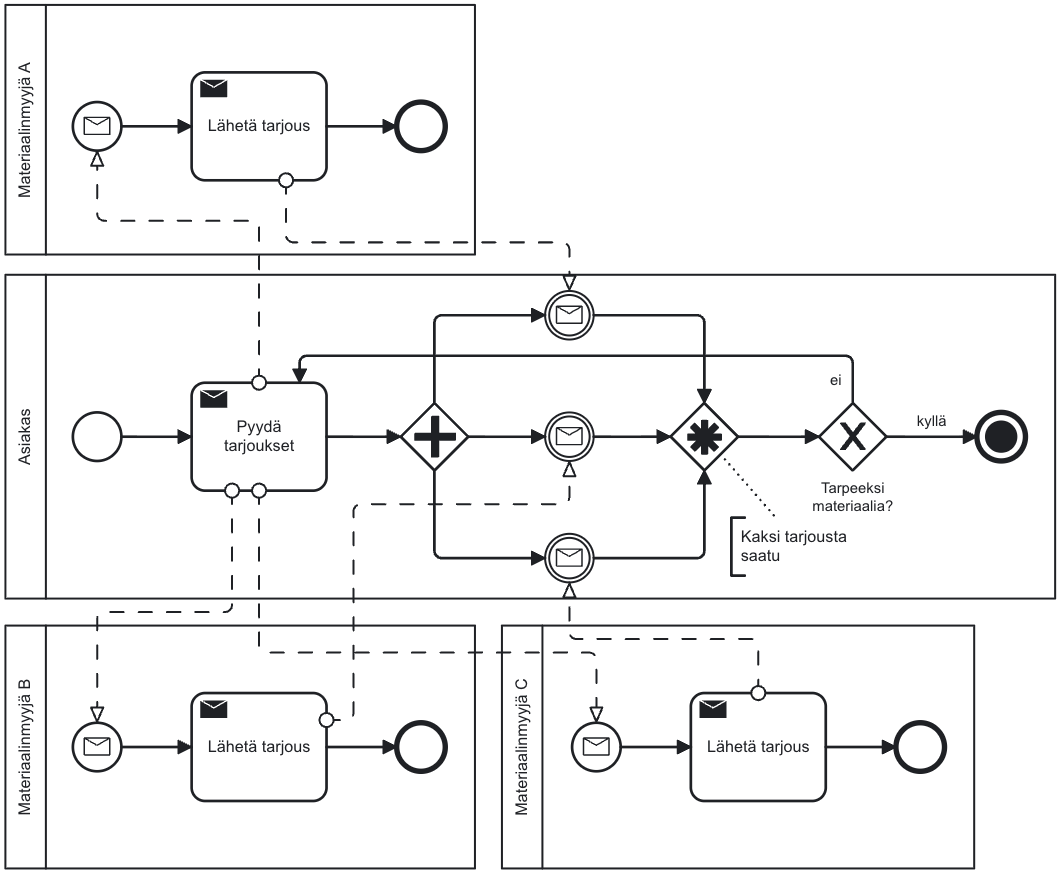
\includegraphics[keepaspectratio]{kuviot/complex-esim.png}}

}

\caption{\label{fig-complex-esim-teht}Complex Gateway -portti
tarjouspyyntöprosessissa}

\end{figure}%

\begin{tcolorbox}[enhanced jigsaw, arc=.35mm, bottomrule=.15mm, bottomtitle=1mm, breakable, colback=white, colbacktitle=quarto-callout-tip-color!10!white, colframe=quarto-callout-tip-color-frame, coltitle=black, left=2mm, leftrule=.75mm, opacityback=0, opacitybacktitle=0.6, rightrule=.15mm, title=\textcolor{quarto-callout-tip-color}{\faLightbulb}\hspace{0.5em}{Malliratkaisu}, titlerule=0mm, toprule=.15mm, toptitle=1mm]

Yksi ratkaisu: Parallel Gatewayn jälkeen jokaisesta kolmesta Message
Intermediate Catch Eventistä ''Tarjous saapunut'' jatketaan Script
Taskiin \emph{Kasvata tarjouslaskuria}. Haarat yhdistetään Exclusive
Gatewaylla, jonka jälkeen Exclusive Gateway ''Kaksi tarjousta saatu?''.
Ehto \texttt{tarjouksia\ =\ 2} vie tarkistukseen ''Tarpeeksi
materiaalia?''. Oletusvirta päättyy tavalliseen End Eventiin, joka
lopettaa vain kyseisen haaran. Ehto on \texttt{=\ 2} eikä
\texttt{\textgreater{}=\ 2}, jotta kolmas tarjous ei käynnistä jatkoa
uudelleen.

Ratkaisussa on ongelma: jos kolmatta tarjousta ei koskaan tule, sen
haara jää odottamaan, eikä prosessi-instanssi pääty. Tämän voi korjata
esimerkiksi ajastimella tai päättämällä prosessin Terminate End
Eventillä. Selkeämpi vaihtoehto on Parallel Multi-Instance -tyyppinen
Receive Task \emph{Vastaanota tarjous}, jolla on kolme instanssia ja
päättymisehto \texttt{nrOfCompletedInstances\ \textgreater{}=\ 2}. Kun
kaksi tarjousta on saatu, tehtävä päättyy ja kolmannen tarjouksen odotus
perutaan.

Kummassakin mallissa kannattaa miettiä, mitä tapahtuu, kun materiaalia
ei ole tarpeeksi ja tarjouksia pyydetään uudelleen. Kuvan mallissa paluu
tapahtuu silloin, kun kolmannen tarjouksen odotus voi olla vielä kesken.

\end{tcolorbox}

\subsection{Tapahtumat}\label{tapahtumat-1}

\subsubsection{BPMN-tehtävä 22}\label{bpmn-tehtuxe4vuxe4-22}

Joka arkipäivä kello kahdeksan järjestelmä kokoaa edellisen päivän
tilaukset raportiksi ja lähettää sen myyntipäällikölle. Mallinna
prosessi. Millä tapahtumalla prosessi käynnistyy?

\begin{tcolorbox}[enhanced jigsaw, arc=.35mm, bottomrule=.15mm, bottomtitle=1mm, breakable, colback=white, colbacktitle=quarto-callout-tip-color!10!white, colframe=quarto-callout-tip-color-frame, coltitle=black, left=2mm, leftrule=.75mm, opacityback=0, opacitybacktitle=0.6, rightrule=.15mm, title=\textcolor{quarto-callout-tip-color}{\faLightbulb}\hspace{0.5em}{Malliratkaisu}, titlerule=0mm, toprule=.15mm, toptitle=1mm]

Timer Start Event → \emph{Kokoa tilausraportti} (Script tai Service
Task) → \emph{Lähetä raportti myyntipäällikölle} (Send Task) → End
Event. Pelkällä ISO 8601 -toistomääreellä ei voi rajata toistoa
arkipäiviin. Esimerkiksi Camunda hyväksyy ajastimelle myös
cron-lausekkeen, jolla arkipäivät voi määritellä.

\end{tcolorbox}

\subsubsection{BPMN-tehtävä 23}\label{bpmn-tehtuxe4vuxe4-23}

Sämpylätaikinan vaivaamisen jälkeen taikinan annetaan kohota 45
minuuttia. Sitten sämpylät leivotaan ja niiden annetaan kohota vielä 20
minuuttia, minkä jälkeen ne paistetaan. Mallinna prosessi ja kirjoita
odotusajat ISO 8601 -muodossa.

\begin{tcolorbox}[enhanced jigsaw, arc=.35mm, bottomrule=.15mm, bottomtitle=1mm, breakable, colback=white, colbacktitle=quarto-callout-tip-color!10!white, colframe=quarto-callout-tip-color-frame, coltitle=black, left=2mm, leftrule=.75mm, opacityback=0, opacitybacktitle=0.6, rightrule=.15mm, title=\textcolor{quarto-callout-tip-color}{\faLightbulb}\hspace{0.5em}{Malliratkaisu}, titlerule=0mm, toprule=.15mm, toptitle=1mm]

\emph{Vaivaa taikina} → Timer Intermediate Catch Event \texttt{PT45M} →
\emph{Leivo sämpylät} → Timer Intermediate Catch Event \texttt{PT20M} →
\emph{Paista sämpylät} → End Event. Kohoaminen ei ole kenenkään tekemä
tehtävä vaan odotusta, joten se esitetään ajastintapahtumana.

\end{tcolorbox}

\subsubsection{BPMN-tehtävä 24}\label{bpmn-tehtuxe4vuxe4-24}

Pizzerian lupaus on, että pizza toimitetaan tunnissa. Jos toimitus
kestää yli tunnin, asiakkaalle lähetetään alennuskoodi seuraavaa
tilausta varten, mutta toimitus jatkuu normaalisti. Mallinna toimitus.
Miten prosessin kulku muuttuisi, jos käyttäisit keskeyttävää ajastinta?

\begin{tcolorbox}[enhanced jigsaw, arc=.35mm, bottomrule=.15mm, bottomtitle=1mm, breakable, colback=white, colbacktitle=quarto-callout-tip-color!10!white, colframe=quarto-callout-tip-color-frame, coltitle=black, left=2mm, leftrule=.75mm, opacityback=0, opacitybacktitle=0.6, rightrule=.15mm, title=\textcolor{quarto-callout-tip-color}{\faLightbulb}\hspace{0.5em}{Malliratkaisu}, titlerule=0mm, toprule=.15mm, toptitle=1mm]

Tehtävään \emph{Toimita pizza} liitetään ei-keskeyttävä (katkoviivainen)
Timer Boundary Event \texttt{PT1H}. Siitä lähtee haara \emph{Lähetä
alennuskoodi} → End Event. Pääpolku jatkuu tehtävästä \emph{Toimita
pizza} omaan End Eventiinsä. Keskeyttävä ajastin pysäyttäisi toimituksen
tunnin kohdalla, eli pizza jäisi toimittamatta.

\end{tcolorbox}

\subsubsection{BPMN-tehtävä 25}\label{bpmn-tehtuxe4vuxe4-25}

Verkkokaupan asiakkaalla on 15 minuuttia aikaa maksaa tilauksensa. Jos
maksua ei kuulu, tuotteiden varaus perutaan. Mallinna prosessi Receive
Taskin ja ajastimen avulla.

\begin{tcolorbox}[enhanced jigsaw, arc=.35mm, bottomrule=.15mm, bottomtitle=1mm, breakable, colback=white, colbacktitle=quarto-callout-tip-color!10!white, colframe=quarto-callout-tip-color-frame, coltitle=black, left=2mm, leftrule=.75mm, opacityback=0, opacitybacktitle=0.6, rightrule=.15mm, title=\textcolor{quarto-callout-tip-color}{\faLightbulb}\hspace{0.5em}{Malliratkaisu}, titlerule=0mm, toprule=.15mm, toptitle=1mm]

\emph{Varaa tuotteet} → Receive Task \emph{Vastaanota maksu}, johon
liitetään keskeyttävä Timer Boundary Event \texttt{PT15M}. Pääpolku:
\emph{Vastaanota maksu} → \emph{Vahvista tilaus} → End Event. Ajastimen
polku: \emph{Peru varaus} → End Event. Tässä keskeyttävä ajastin on
oikea valinta, koska maksun odottaminen halutaan lopettaa.

\end{tcolorbox}

\subsubsection{BPMN-tehtävä 26}\label{bpmn-tehtuxe4vuxe4-26}

Hammaslääkärin vastaanotolle saapuu ajanvarauspyyntö verkkolomakkeen
kautta. Vastaanoton sihteeri varaa ajan kalenterista, minkä jälkeen
asiakkaalle lähetetään vahvistus. Mallinna prosessi viestitapahtumien
avulla.

\begin{tcolorbox}[enhanced jigsaw, arc=.35mm, bottomrule=.15mm, bottomtitle=1mm, breakable, colback=white, colbacktitle=quarto-callout-tip-color!10!white, colframe=quarto-callout-tip-color-frame, coltitle=black, left=2mm, leftrule=.75mm, opacityback=0, opacitybacktitle=0.6, rightrule=.15mm, title=\textcolor{quarto-callout-tip-color}{\faLightbulb}\hspace{0.5em}{Malliratkaisu}, titlerule=0mm, toprule=.15mm, toptitle=1mm]

Message Start Event ''Ajanvarauspyyntö saapunut'' → User Task
\emph{Varaa aika kalenterista} → Message End Event ''Vahvistus
lähetetty''. Viestitapahtumat kertovat, että prosessi käynnistyy
ulkoisesta viestistä ja päättyy viestin lähettämiseen.

\end{tcolorbox}

\subsubsection{BPMN-tehtävä 27}\label{bpmn-tehtuxe4vuxe4-27}

Yritys lähettää asiakkaalle tarjouksen. Jos asiakas hyväksyy tarjouksen,
tehdään tilaus. Jos asiakas hylkää sen, hylkäys kirjataan. Jos
asiakkaalta ei kuulu mitään kahteen viikkoon, myyjä soittaa hänelle.
Mallinna tilanne.

\begin{tcolorbox}[enhanced jigsaw, arc=.35mm, bottomrule=.15mm, bottomtitle=1mm, breakable, colback=white, colbacktitle=quarto-callout-tip-color!10!white, colframe=quarto-callout-tip-color-frame, coltitle=black, left=2mm, leftrule=.75mm, opacityback=0, opacitybacktitle=0.6, rightrule=.15mm, title=\textcolor{quarto-callout-tip-color}{\faLightbulb}\hspace{0.5em}{Malliratkaisu}, titlerule=0mm, toprule=.15mm, toptitle=1mm]

\emph{Lähetä tarjous} → Event-Based Gateway, jota seuraa kolme
tapahtumaa: Message Intermediate Catch Event ''Hyväksyntä saapunut'' →
\emph{Tee tilaus}, Message Intermediate Catch Event ''Hylkäys saapunut''
→ \emph{Kirjaa hylkäys} ja Timer Intermediate Catch Event \texttt{P14D}
→ \emph{Soita asiakkaalle}. Ensimmäisenä toteutuva tapahtuma ratkaisee
polun.

\end{tcolorbox}

\subsubsection{BPMN-tehtävä 28}\label{bpmn-tehtuxe4vuxe4-28}

Kassalla asiakkaan maksukortti veloitetaan. Jos maksupalvelu hylkää
kortin, asiakkaalta pyydetään toinen maksutapa. Mallinna virhetilanne
Error Eventin avulla. Voiko virhetapahtuma olla ei-keskeyttävä?

\begin{tcolorbox}[enhanced jigsaw, arc=.35mm, bottomrule=.15mm, bottomtitle=1mm, breakable, colback=white, colbacktitle=quarto-callout-tip-color!10!white, colframe=quarto-callout-tip-color-frame, coltitle=black, left=2mm, leftrule=.75mm, opacityback=0, opacitybacktitle=0.6, rightrule=.15mm, title=\textcolor{quarto-callout-tip-color}{\faLightbulb}\hspace{0.5em}{Malliratkaisu}, titlerule=0mm, toprule=.15mm, toptitle=1mm]

Service Task \emph{Veloita kortti}, johon liitetään Error Boundary Event
(virhekoodi esimerkiksi \texttt{KORTTI\_HYLATTY}) → \emph{Pyydä toinen
maksutapa}. Pääpolku jatkuu tehtävästä \emph{Veloita kortti} tehtävään
\emph{Anna kuitti}. Error Boundary Event on aina keskeyttävä: virhe
lopettaa tehtävän suorittamisen.

\end{tcolorbox}

\subsubsection{BPMN-tehtävä 29}\label{bpmn-tehtuxe4vuxe4-29}

Perhe etsii kadonnutta kissaa. Yksi perheenjäsen etsii pihalta ja toinen
läheisestä metsästä samaan aikaan. Kun kissa löytyy, kaikki etsiminen
lopetetaan. Mallinna prosessi. Mikä ero on End Eventillä ja Terminate
End Eventillä tässä tilanteessa?

\begin{tcolorbox}[enhanced jigsaw, arc=.35mm, bottomrule=.15mm, bottomtitle=1mm, breakable, colback=white, colbacktitle=quarto-callout-tip-color!10!white, colframe=quarto-callout-tip-color-frame, coltitle=black, left=2mm, leftrule=.75mm, opacityback=0, opacitybacktitle=0.6, rightrule=.15mm, title=\textcolor{quarto-callout-tip-color}{\faLightbulb}\hspace{0.5em}{Malliratkaisu}, titlerule=0mm, toprule=.15mm, toptitle=1mm]

\emph{Huomaa kissa kadonneeksi} → Parallel Gateway → kaksi haaraa:
\emph{Etsi pihalta} ja \emph{Etsi metsästä}. Kumpikin haara päättyy
Terminate End Eventiin ''Kissa löytyi''. Tavallinen End Event lopettaisi
vain oman haaransa, ja toinen perheenjäsen jatkaisi etsimistä turhaan.

\end{tcolorbox}

\subsubsection{BPMN-tehtävä 30}\label{bpmn-tehtuxe4vuxe4-30}

Toimistorakennuksen turvallisuuspäällikkö käynnistää palohälytyksen.
Rakennuksen jokaisessa kerroksessa käynnistyy oma evakuointiprosessi:
kerroksen henkilökunta poistuu rakennuksesta ja ilmoittautuu
kokoontumispaikalla. Mallinna tilanne. Miksi Message Event ei sovi
tähän?

\begin{tcolorbox}[enhanced jigsaw, arc=.35mm, bottomrule=.15mm, bottomtitle=1mm, breakable, colback=white, colbacktitle=quarto-callout-tip-color!10!white, colframe=quarto-callout-tip-color-frame, coltitle=black, left=2mm, leftrule=.75mm, opacityback=0, opacitybacktitle=0.6, rightrule=.15mm, title=\textcolor{quarto-callout-tip-color}{\faLightbulb}\hspace{0.5em}{Malliratkaisu}, titlerule=0mm, toprule=.15mm, toptitle=1mm]

Turvallisuuspäällikön prosessi: \emph{Havaitse palo} → Signal
Intermediate Throw Event ''Palohälytys''. Kunkin kerroksen prosessi:
Signal Start Event ''Palohälytys'' → \emph{Poistu rakennuksesta} →
\emph{Ilmoittaudu kokoontumispaikalla} → End Event. Signaali välitetään
kaikille sitä kuunteleville, eikä lähettäjän tarvitse tietää, montako
vastaanottajaa on. Viesti sen sijaan osoitetaan aina yhdelle tietylle
vastaanottajalle.

\end{tcolorbox}

\subsubsection{BPMN-tehtävä 31}\label{bpmn-tehtuxe4vuxe4-31}

Miten seuraavat prosessimallit tulkitaan?

\begin{figure}

\centering{

\pandocbounded{\includegraphics[keepaspectratio]{index_files/mediabag/kuviot/timer_esim.pdf}}

}

\caption{\label{fig-timer_esim-teht}Esimerkkejä Timer-tapahtuman
käytöstä}

\end{figure}%

\begin{tcolorbox}[enhanced jigsaw, arc=.35mm, bottomrule=.15mm, bottomtitle=1mm, breakable, colback=white, colbacktitle=quarto-callout-tip-color!10!white, colframe=quarto-callout-tip-color-frame, coltitle=black, left=2mm, leftrule=.75mm, opacityback=0, opacitybacktitle=0.6, rightrule=.15mm, title=\textcolor{quarto-callout-tip-color}{\faLightbulb}\hspace{0.5em}{Malliratkaisu}, titlerule=0mm, toprule=.15mm, toptitle=1mm]

\begin{enumerate}
\def\labelenumi{\arabic{enumi}.}
\tightlist
\item
  Prosessi käynnistyy arkipäivisin klo 06:45 (toistuva Timer Start
  Event, esimerkiksi cron-lausekkeella). Aamutoimien jälkeen odotetaan
  kello 07:30 asti ja lähdetään töihin. Jos aamutoimet venyvät yli
  07:30, ajastimen määrittely ratkaisee, lähdetäänkö heti vai
  odotetaanko seuraavaan kertaan. Siksi ajankohta kannattaa määritellä
  suhteessa instanssin päivämäärään.
\item
  Joka tunti käynnistyy uusi prosessi-instanssi, jossa luetaan
  sähköpostit. Sen jälkeen jokainen instanssi odottaa päiväkahvitaukoa
  ennen kuin sähköposteihin vastataan. Päivän aikana kertyy siis useita
  odottavia instansseja, jotka kaikki jatkuvat samaan aikaan
  kahvitauolla. Tämä tuskin on tarkoitus. ''Päiväkahvitauko'' ei
  myöskään ole ajastimen määrittely, vaan se pitää ilmaista
  kellonaikana.
\item
  Aloitusajastin ''Kuukausi ennen matkaa'' edellyttää, että matkan
  päivämäärä tunnetaan ennen kuin prosessi on olemassa. Aloitustapahtuma
  ei voi lukea prosessimuuttujia, joten parempi aloitus olisi
  esimerkiksi ''Matka päätetty'', jonka jälkeen odotus lasketaan matkan
  päivämäärästä välitapahtumalla. Välitapahtuma ''Päivä ennen matkaa''
  toimii, kun sen ajankohta lasketaan matkan päivämäärän sisältävästä
  muuttujasta.
\item
  Kertaluonteinen aloitus 19.5.2027 klo 05:15. Lähtötoimien aikana
  ei-keskeyttävä reuna-ajastin laukeaa 45 minuuttia ennen lähtöä eli klo
  05:45 (\texttt{PT30M} tehtävän alkamisesta), ja taksi tilataan
  lähtötoimien jatkuessa. Pääpolulla odotetaan klo 06:30 asti ja
  lähdetään. Mallissa on kaksi ongelmaa: (a) \emph{Lähde lentokentälle}
  -tehtävään saapuu kaksi järjestysvirtaa ilman porttia, joten tehtävä
  suoritetaan kahdesti, ja (b) jos lähtötoimet valmistuvat ennen klo
  05:45, reuna-ajastin ei laukea lainkaan, eikä taksia tilata. Korjaus:
  taksin tilaus omaksi rinnakkaiseksi haarakseen ja haarojen
  yhdistäminen Parallel Gatewaylla ennen lähtöä.
\end{enumerate}

\end{tcolorbox}

\subsubsection{BPMN-tehtävä 32}\label{bpmn-tehtuxe4vuxe4-32}

\begin{enumerate}
\def\labelenumi{\arabic{enumi}.}
\tightlist
\item
  Ilmaise vuoden 2026 viikon 42 maanantai ISO 8601 -standardin mukaisena
  päivämääränä käyttäen viikkonumerointia. Mikä kalenteripäivä se on?
\item
  Muunna tapahtuma, joka alkaa 2025-12-06 klo 09:00 Suomen aikaa
  (Europe/Helsinki), ISO 8601 -muotoon sisältäen aikavyöhykkeen
  poikkeaman (offset) sekä UTC-vastineen.
\item
  Esitä 2 tuntia 30 minuuttia ISO 8601 -keston merkintänä. Esitä sitten
  kesto, johon on lisätty 15 minuutin tauko.
\item
  Kurssin intensiiviviikolla opiskellaan maanantaista 4.1.2027
  torstaihin 7.1.2027 joka päivä klo 09:00--16:00. Esitä opiskelujaksot
  ISO 8601 -muodossa. Miksi yksi aikaväli
  \texttt{2027-01-04T09:00/2027-01-07T16:00} ei kuvaa tilannetta oikein?
\item
  Esitä viikoittainen palaveri, joka pidetään keskiviikkoisin klo
  12:00--12:45 tammi--maaliskuussa 2027, ISO 8601 -muotoisena toistuvana
  aikavälinä. Mitä toistuvuuden ilmaisemisessa pitää ottaa huomioon
  maaliskuun lopussa?
\end{enumerate}

\begin{tcolorbox}[enhanced jigsaw, arc=.35mm, bottomrule=.15mm, bottomtitle=1mm, breakable, colback=white, colbacktitle=quarto-callout-tip-color!10!white, colframe=quarto-callout-tip-color-frame, coltitle=black, left=2mm, leftrule=.75mm, opacityback=0, opacitybacktitle=0.6, rightrule=.15mm, title=\textcolor{quarto-callout-tip-color}{\faLightbulb}\hspace{0.5em}{Malliratkaisu}, titlerule=0mm, toprule=.15mm, toptitle=1mm]

\begin{enumerate}
\def\labelenumi{\arabic{enumi}.}
\tightlist
\item
  \texttt{2026-W42-1} eli maanantai 12.10.2026 (\texttt{2026-10-12}).
\item
  \texttt{2025-12-06T09:00:00+02:00}. UTC-aikana
  \texttt{2025-12-06T07:00:00Z}. Joulukuussa Suomessa on normaaliaika,
  joten ero UTC-aikaan on kaksi tuntia.
\item
  \texttt{PT2H30M}. Tauon kanssa \texttt{PT2H45M}. Kestoja ei kirjoiteta
  peräkkäin, vaan ne lasketaan yhteen yhdeksi kestoksi.
\item
  Opiskelujaksoja on neljä erillistä: \texttt{2027-01-04T09:00/16:00},
  \texttt{2027-01-05T09:00/16:00}, \texttt{2027-01-06T09:00/16:00} ja
  \texttt{2027-01-07T09:00/16:00} (aikavälin loppuosasta voi jättää pois
  alkuosan kanssa yhteiset osat). Yksi aikaväli maanantaiaamusta
  torstai-iltapäivään sisältäisi myös illat ja yöt. Toistomerkintä
  \texttt{R4/2027-01-04T09:00:00+02:00/P1D} antaa jaksojen alkamisajat,
  mutta ei jakson pituutta. Huomaa, että merkintä
  \texttt{R4/2027-01-04T09:00/PT7H} olisi väärin, sillä toistuvat
  aikavälit seuraavat toisiaan katkeamatta (09--16, 16--23, 23--06 ja
  niin edelleen).
\item
  Ensimmäinen palaveri on keskiviikkona 6.1.2027, ja palavereja on 13:
  \texttt{R13/2027-01-06T12:00:00+02:00/P1W}. Palaverin kesto
  \texttt{PT45M} ilmoitetaan erikseen. Kesäaika alkaa sunnuntaina
  28.3.2027, joten kiinteä poikkeama \texttt{+02:00} siirtäisi viimeisen
  palaverin (31.3.) Suomen aikaa klo 13:00:aan. Oikea aika olisi
  \texttt{2027-03-31T12:00:00+03:00}. ISO 8601:n perusmerkinnöillä ei
  voi ilmaista sääntöä ''joka keskiviikko aikavyöhykkeen paikallista
  aikaa''. Siihen käytetään esimerkiksi kalenterisovellusten
  iCalendar-standardin toistosääntöä
  (\texttt{RRULE:FREQ=WEEKLY;BYDAY=WE;UNTIL=20270331T235959Z} yhdessä
  aikavyöhykkeen \texttt{Europe/Helsinki} kanssa).
\end{enumerate}

\end{tcolorbox}

\subsubsection{BPMN-tehtävä 33
(laajempi)}\label{bpmn-tehtuxe4vuxe4-33-laajempi}

Piirrä seuraava prosessikulku. Asiakas lähettää palvelupisteelle
tukipyynnön. Ensimmäiseksi tarkastetaan, sisältääkö tukipyyntö kaikki
tarvittavat tiedot asian käsittelemiseksi. Mikäli lisätietoja ei
tarvita, tukipyyntö ohjataan ratkaistavaksi ja prosessi lopetetaan. Jos
lisätietoja tarvitaan, näitä pyydetään asiakkaalta. Kun asiakas
toimittaa lisätiedot, tukipyyntö ohjataan ratkaistavaksi ja prosessi
lopetetaan. Mikäli asiakas ei ole toimittanut lisätietoja 48 tunnin
kuluessa, tukipyyntö hylätään ja prosessi lopetetaan.

Tee edellisestä prosessista versio, jossa asiakasta muistutetaan, ellei
hän ole toimittanut tarvittavia lisätietoja 48 tunnin kuluessa. Tämän
jälkeen lisätietoja odotetaan toiset 48 tuntia ennen tukipyynnön
hylkäämistä.

Tee edellisestä prosessista versio, jossa asiakasta muistutetaan
lisätiedoista 48 tunnin kuluttua. Sitten asiakasta muistutetaan
tarvittaessa uudelleen 96 tunnin kuluttua. Ellei asiakas ole toimittanut
lisätietoja 270 tunnin kuluttua, tukipyyntö hylätään ja prosessi
lopetetaan.

\begin{tcolorbox}[enhanced jigsaw, arc=.35mm, bottomrule=.15mm, bottomtitle=1mm, breakable, colback=white, colbacktitle=quarto-callout-tip-color!10!white, colframe=quarto-callout-tip-color-frame, coltitle=black, left=2mm, leftrule=.75mm, opacityback=0, opacitybacktitle=0.6, rightrule=.15mm, title=\textcolor{quarto-callout-tip-color}{\faLightbulb}\hspace{0.5em}{Malliratkaisu}, titlerule=0mm, toprule=.15mm, toptitle=1mm]

\textbf{Versio 1}: Message Start Event ''Tukipyyntö vastaanotettu'' →
\emph{Tarkista tukipyynnön tiedot} → Exclusive Gateway ''Lisätietoja
tarvitaan?''. Haara ''Ei'' → yhdistävä Exclusive Gateway → \emph{Ohjaa
tukipyyntö ratkaistavaksi} → End Event. Haara ''Kyllä'' → Send Task
\emph{Pyydä lisätietoja asiakkaalta} → Receive Task \emph{Vastaanota
lisätiedot} → yhdistävä portti. Receive Taskiin liitetään keskeyttävä
Timer Boundary Event \texttt{PT48H} → \emph{Hylkää tukipyyntö} → End
Event ''Tukipyyntö hylätty''. Saman voi mallintaa myös Event-Based
Gatewaylla, jota seuraavat Message Intermediate Catch Event ja Timer
Intermediate Catch Event.

\textbf{Versio 2}: Receive Taskiin liitetään kaksi reuna-ajastinta:
ei-keskeyttävä \texttt{PT48H} → Send Task \emph{Muistuta asiakasta} →
End Event sekä keskeyttävä \texttt{PT96H} → \emph{Hylkää tukipyyntö}.
Molemmat ajat lasketaan siitä hetkestä, kun tehtävä alkoi, joten
hylkäysajastin on 96 tuntia eikä 48. Ei-keskeyttävä ajastin jättää
lisätietojen odotuksen voimaan.

\textbf{Versio 3}: Kuten versio 2, mutta ei-keskeyttäviä
muistutusajastimia on kaksi (\texttt{PT48H} ja \texttt{PT96H}) tai yksi
toistuva ajastin \texttt{R2/PT48H}, ja keskeyttävä hylkäysajastin on
\texttt{PT270H} (eli \texttt{P11DT6H}).

\end{tcolorbox}

\subsubsection{BPMN-tehtävä 34}\label{bpmn-tehtuxe4vuxe4-34}

Lisää seuraavaan prosessiin ei-keskeyttävä Message Boundary Event, joka
ottaa vastaan asiakkaan tilaukseensa tekemän muutoksen, sekä sen
käynnistämä polku.

\begin{figure}

\centering{

\pandocbounded{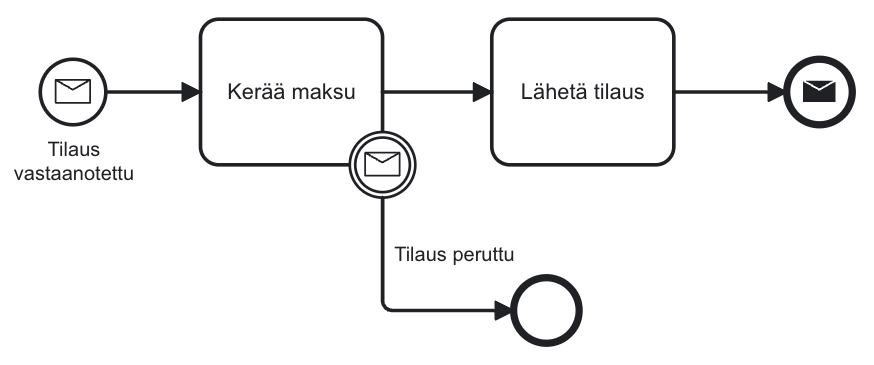
\includegraphics[keepaspectratio]{kuviot/eventteja3.png}}

}

\caption{\label{fig-eventteja3-teht}Message Start Event, Message
Intermediate Boundary Event ja Message End Event}

\end{figure}%

\begin{tcolorbox}[enhanced jigsaw, arc=.35mm, bottomrule=.15mm, bottomtitle=1mm, breakable, colback=white, colbacktitle=quarto-callout-tip-color!10!white, colframe=quarto-callout-tip-color-frame, coltitle=black, left=2mm, leftrule=.75mm, opacityback=0, opacitybacktitle=0.6, rightrule=.15mm, title=\textcolor{quarto-callout-tip-color}{\faLightbulb}\hspace{0.5em}{Malliratkaisu}, titlerule=0mm, toprule=.15mm, toptitle=1mm]

Tehtävään \emph{Kerää maksu} liitetään ei-keskeyttävä (katkoviivainen)
Message Boundary Event ''Muutospyyntö saapunut'' → \emph{Päivitä tilaus}
→ \emph{Lähetä muutosvahvistus} → End Event ''Muutos käsitelty''. Maksun
kerääminen jatkuu muutoksen käsittelyn ajan. Huomaa, että reunatapahtuma
on voimassa vain tehtävän \emph{Kerää maksu} ajan. Jos muutoksia
halutaan ottaa vastaan koko tilauksen käsittelyn ajan, tehtävät voidaan
koota aliprosessiksi ja liittää tapahtuma siihen, tai käyttää
ei-keskeyttävää tapahtuma-aliprosessia (Event Sub-Process). Jos muutos
vaikuttaa hintaan, kannattaa pohtia, pitäisikö tapahtuman sittenkin
keskeyttää maksun kerääminen.

\end{tcolorbox}

\subsubsection{BPMN-tehtävä 35}\label{bpmn-tehtuxe4vuxe4-35}

Piirrä seuraavasta tapahtumakulusta prosessimalli, jossa hyödynnät
Message Boundary Eventejä.

Prosessi alkaa, kun asiakas lähettää tukipyynnön sähköistä lomaketta
käyttäen. Järjestelmä luo yhteydenoton perusteella tukipyynnön ja
lähettää asiakkaalle vahvistusviestin. Tukihenkilö valmistelee
vastauksen. Jos asiakas vastaa vahvistusviestiin lisätiedoilla kesken
valmistelun, viesti keskeyttää tehtävän ja ohjaa polun ``Lisätietojen
tarkistus'' -aliprosessiin. Jos vastausta ei tule, valmistelu jatkuu
normaalisti ja tukihenkilö lähettää vastauksen. Vastauksen lähetyksen
jälkeen prosessi päättyy.

\begin{tcolorbox}[enhanced jigsaw, arc=.35mm, bottomrule=.15mm, bottomtitle=1mm, breakable, colback=white, colbacktitle=quarto-callout-tip-color!10!white, colframe=quarto-callout-tip-color-frame, coltitle=black, left=2mm, leftrule=.75mm, opacityback=0, opacitybacktitle=0.6, rightrule=.15mm, title=\textcolor{quarto-callout-tip-color}{\faLightbulb}\hspace{0.5em}{Malliratkaisu}, titlerule=0mm, toprule=.15mm, toptitle=1mm]

Message Start Event ''Tukipyyntö lähetetty'' → Service Task \emph{Luo
tukipyyntö} → Send Task \emph{Lähetä vahvistusviesti} → yhdistävä
Exclusive Gateway → User Task \emph{Valmistele vastaus} → Send Task
\emph{Lähetä vastaus} → End Event ''Vastaus lähetetty''.

Tehtävään \emph{Valmistele vastaus} liitetään keskeyttävä Message
Boundary Event ''Lisätiedot saapuneet'' → aliprosessi \emph{Lisätietojen
tarkistus} → takaisin yhdistävään porttiin ennen tehtävää
\emph{Valmistele vastaus}. Tehtävänanto ei kerro, mitä aliprosessin
jälkeen tapahtuu. Paluu valmisteluun on luonteva oletus. Jos valmistelua
ei haluta aloittaa alusta, tapahtuma voi olla myös ei-keskeyttävä.

\end{tcolorbox}

\subsubsection{BPMN-tehtävä 36}\label{bpmn-tehtuxe4vuxe4-36}

Piirrä seuraavasta tapahtumakulusta prosessimalli, jossa hyödynnät
ehdollisia tapahtumia.

Kun lasku saapuu, prosessi käynnistyy Message Start Eventillä.
Seuraavaksi lasku tarkistetaan. Jos laskun summa on yli 5 000 € ja
toimittaja ei ole hyväksyttyjen toimittajien listalla, siirrytään
tehtävään ''Hanki lisähyväksyntä''. Muutoin edetään suoraan tehtävään
''Kirjaa lasku''. Jos laskusta puuttuu joitain pakollisten kenttien
tietoja, lasku palautetaan.

\begin{tcolorbox}[enhanced jigsaw, arc=.35mm, bottomrule=.15mm, bottomtitle=1mm, breakable, colback=white, colbacktitle=quarto-callout-tip-color!10!white, colframe=quarto-callout-tip-color-frame, coltitle=black, left=2mm, leftrule=.75mm, opacityback=0, opacitybacktitle=0.6, rightrule=.15mm, title=\textcolor{quarto-callout-tip-color}{\faLightbulb}\hspace{0.5em}{Malliratkaisu}, titlerule=0mm, toprule=.15mm, toptitle=1mm]

Message Start Event ''Lasku saapunut'' → \emph{Tarkista lasku} →
Exclusive Gateway. Ehto
\texttt{summa\ \textgreater{}\ 5000\ and\ not\ hyväksyttyToimittaja} →
\emph{Hanki lisähyväksyntä} → yhdistävä portti. Oletusvirta → suoraan
yhdistävään porttiin. Portin jälkeen \emph{Kirjaa lasku} → End Event.

Puuttuvat tiedot voidaan mallintaa keskeyttävällä Conditional Boundary
Eventillä tehtävässä \emph{Tarkista lasku}. Ehto
\texttt{puuttuviaKenttiä\ =\ true} → \emph{Palauta lasku} → End Event
''Lasku palautettu''. Ehdollinen tapahtuma laukeaa heti, kun ehto
täyttyy, vaikka tarkistus olisi vielä kesken.

Pohdittavaa: ehdolliset tapahtumat sopivat tilanteisiin, joissa ehto voi
täyttyä milloin tahansa odotuksen tai tehtävän aikana. Tehtävän jälkeen
tehtävä tietoon perustuva valinta on yleensä selkeintä mallintaa
Exclusive Gatewaylla. Lisähyväksynnän tarpeen voi mallintaa ehdollisilla
välitapahtumilla, mutta silloin pitää varmistaa, että täsmälleen yksi
ehto täyttyy.

\end{tcolorbox}

\subsubsection{BPMN-tehtävä 37
(laajempi)}\label{bpmn-tehtuxe4vuxe4-37-laajempi}

Ajatellaan jotain systeemiä, jolla on useita samanaikaisia käyttäjiä.
Yksi käyttäjistä käynnistää prosessin, jossa prosessimuuttujan
\texttt{luku1} numeroarvosta siirretään puolet muuttujan \texttt{luku2}
arvoon. Jokin tehtävä lukee ensin \texttt{luku1}:n lähtöarvon ja
vähentää siitä puolet. Mikäli \texttt{luku2}:n arvon kasvattaminen
\texttt{luku1}:n puolikkaalla jostain teknisestä tai vaikka
liiketoimintasääntöön perustuvasta syystä kuitenkin epäonnistuu,
transaktiomuotoisessa suorituksessa prosessi keskeytetään (\emph{Abort})
ja systeemi palautetaan sen alkuperäiseen tilaan (\emph{Rollback}). On
kuitenkin mahdollista, että systeemin toinen käyttäjä on tällä välin
päivittänyt \texttt{luku1}:n arvoa, jolloin alkuperäisen tilan
palauttaminen rollback-operaatiolla hävittää myös toisen käyttäjän
tekemän muutoksen.

Suunnittele kompensoiva rakenne, joka pitää systeemin tietojen arvot
oikeina kaikissa tapauksissa.

Toimiiko suunnittelemasi kompensaatio, mikäli \texttt{luku1}:n arvo ei
saa koskaan mennä alle nollan?

\begin{tcolorbox}[enhanced jigsaw, arc=.35mm, bottomrule=.15mm, bottomtitle=1mm, breakable, colback=white, colbacktitle=quarto-callout-tip-color!10!white, colframe=quarto-callout-tip-color-frame, coltitle=black, left=2mm, leftrule=.75mm, opacityback=0, opacitybacktitle=0.6, rightrule=.15mm, title=\textcolor{quarto-callout-tip-color}{\faLightbulb}\hspace{0.5em}{Malliratkaisu}, titlerule=0mm, toprule=.15mm, toptitle=1mm]

Rollbackin sijaan käytetään kompensaatiota, joka kumoaa vain prosessin
oman muutoksen. Tehtävä \emph{Vähennä luku1:stä puolet} tallentaa
vähennetyn määrän prosessimuuttujaan \texttt{d} ja vähentää sen yhtenä
atomisena operaationa (\texttt{luku1\ =\ luku1\ −\ d}). Tehtävään
liitetään Compensation Boundary Event, johon kytketään
kompensaatiotehtävä \emph{Palauta d luku1:een}
(\texttt{luku1\ =\ luku1\ +\ d}). Tehtävään \emph{Kasvata luku2:ta
d:llä} liitetään Error Boundary Event, josta jatketaan Compensation
Throw Eventiin. Se käynnistää kompensaation ja prosessi päättyy. Koska
kompensaatio lisää arvoon suhteellisen määrän eikä palauta vanhaa arvoa,
toisen käyttäjän tekemä muutos säilyy.

Nollarajoite: kompensaatio vain kasvattaa \texttt{luku1}:n arvoa, joten
se ei itse voi viedä arvoa alle nollan. Rajoite on kuitenkin
tarkistettava vähennyksen yhteydessä samassa atomisessa operaatiossa
(vähennetään vain, jos \texttt{luku1\ \textgreater{}=\ d}). Jos arvo
luetaan ja vähennetään erikseen, toinen käyttäjä voi muuttaa sitä
välissä. Jos järjestys olisi päinvastainen ja kompensaatio vähentäisi
arvoa, nollarajoite voisi estää kompensaation, ja silloin tarvittaisiin
erillinen poikkeuskäsittely.

\end{tcolorbox}

\subsection{Altaat, viestit ja tieto}\label{altaat-viestit-ja-tieto}

\subsubsection{BPMN-tehtävä 38}\label{bpmn-tehtuxe4vuxe4-38}

Opiskelija tilaa opintorekisteriotteen opintotoimistosta. Opintotoimisto
tulostaa otteen ja lähettää sen opiskelijalle, joka vastaanottaa sen.
Mallinna prosessi kahtena uima-altaana.

\begin{tcolorbox}[enhanced jigsaw, arc=.35mm, bottomrule=.15mm, bottomtitle=1mm, breakable, colback=white, colbacktitle=quarto-callout-tip-color!10!white, colframe=quarto-callout-tip-color-frame, coltitle=black, left=2mm, leftrule=.75mm, opacityback=0, opacitybacktitle=0.6, rightrule=.15mm, title=\textcolor{quarto-callout-tip-color}{\faLightbulb}\hspace{0.5em}{Malliratkaisu}, titlerule=0mm, toprule=.15mm, toptitle=1mm]

Altaassa \emph{Opiskelija}: Start Event → \emph{Lähetä otepyyntö} →
\emph{Vastaanota ote} → End Event. Altaassa \emph{Opintotoimisto}:
Message Start Event → \emph{Tulosta ote} → \emph{Lähetä ote} → End
Event. Viestivirrat kulkevat tehtävästä \emph{Lähetä otepyyntö}
opintotoimiston aloitustapahtumaan sekä tehtävästä \emph{Lähetä ote}
tehtävään \emph{Vastaanota ote}.

\end{tcolorbox}

\subsubsection{BPMN-tehtävä 39}\label{bpmn-tehtuxe4vuxe4-39}

Etsi virhe. Mallissa on kaksi uima-allasta, \emph{Asiakas} ja
\emph{Yritys}. Asiakkaan altaan tehtävästä \emph{Maksa lasku} kulkee
järjestysvirta yrityksen altaan tehtävään \emph{Kirjaa maksu}. Mikä
mallissa on vialla, ja miten se korjataan?

\begin{tcolorbox}[enhanced jigsaw, arc=.35mm, bottomrule=.15mm, bottomtitle=1mm, breakable, colback=white, colbacktitle=quarto-callout-tip-color!10!white, colframe=quarto-callout-tip-color-frame, coltitle=black, left=2mm, leftrule=.75mm, opacityback=0, opacitybacktitle=0.6, rightrule=.15mm, title=\textcolor{quarto-callout-tip-color}{\faLightbulb}\hspace{0.5em}{Malliratkaisu}, titlerule=0mm, toprule=.15mm, toptitle=1mm]

Järjestysvirta ei saa ylittää uima-altaan rajaa. Altaiden välinen
vuorovaikutus esitetään viestivirralla. Yrityksen altaaseen tarvitaan
myös viestin vastaanottava elementti, esimerkiksi Message Start Event
tai Receive Task \emph{Vastaanota maksu}, ennen tehtävää \emph{Kirjaa
maksu}.

\end{tcolorbox}

\subsubsection{BPMN-tehtävä 40}\label{bpmn-tehtuxe4vuxe4-40}

Mallinna taksin tilaaminen mobiilisovelluksella omasta näkökulmastasi.
Taksiyhtiön sisäistä prosessia et tunne, joten esitä taksiyhtiö
suljettuna altaana (\emph{black box pool}).

\begin{tcolorbox}[enhanced jigsaw, arc=.35mm, bottomrule=.15mm, bottomtitle=1mm, breakable, colback=white, colbacktitle=quarto-callout-tip-color!10!white, colframe=quarto-callout-tip-color-frame, coltitle=black, left=2mm, leftrule=.75mm, opacityback=0, opacitybacktitle=0.6, rightrule=.15mm, title=\textcolor{quarto-callout-tip-color}{\faLightbulb}\hspace{0.5em}{Malliratkaisu}, titlerule=0mm, toprule=.15mm, toptitle=1mm]

Oma allas: Start Event → \emph{Tilaa taksi sovelluksella} →
\emph{Vastaanota tilausvahvistus} → \emph{Odota taksia} → \emph{Maksa
matka} → End Event. Taksiyhtiön allas on tyhjä ja suljettu. Viestivirrat
kulkevat tilauksesta suljetun altaan reunaan ja altaan reunasta
vahvistuksen vastaanottoon. Suljettu allas kertoo, että osapuoli on
mukana, mutta sen prosessia ei kuvata.

\end{tcolorbox}

\subsubsection{BPMN-tehtävä 41}\label{bpmn-tehtuxe4vuxe4-41}

Prosessissa on tehtävät \emph{Rekisteröi uusi asiakas} ja \emph{Hae
asiakkaan tiedot}. Lisää malliin Data Store \emph{Asiakasrekisteri} ja
yhdistä se tehtäviin. Kumpi yhteyksistä on Data Input Association ja
kumpi Data Output Association?

\begin{tcolorbox}[enhanced jigsaw, arc=.35mm, bottomrule=.15mm, bottomtitle=1mm, breakable, colback=white, colbacktitle=quarto-callout-tip-color!10!white, colframe=quarto-callout-tip-color-frame, coltitle=black, left=2mm, leftrule=.75mm, opacityback=0, opacitybacktitle=0.6, rightrule=.15mm, title=\textcolor{quarto-callout-tip-color}{\faLightbulb}\hspace{0.5em}{Malliratkaisu}, titlerule=0mm, toprule=.15mm, toptitle=1mm]

\emph{Rekisteröi uusi asiakas} tallentaa tietoa rekisteriin, joten
yhteys kulkee tehtävästä tietovarastoon. Se on Data Output Association,
koska tieto on tehtävän tuotos. \emph{Hae asiakkaan tiedot} lukee
rekisteriä, joten yhteys kulkee tietovarastosta tehtävään. Se on Data
Input Association, koska tieto on tehtävälle syöte.

\end{tcolorbox}

\subsubsection{BPMN-tehtävä 42}\label{bpmn-tehtuxe4vuxe4-42}

Lisää seuraavaan prosessimalliin (kuva~\ref{fig-flow-t}) siitä puuttuvat
Sequence Flow-, Message Flow- ja Data Association -yhteydet.

\begin{figure}

\centering{

\pandocbounded{\includegraphics[keepaspectratio]{index_files/mediabag/kuviot/flow-tehtava_1.pdf}}

}

\caption{\label{fig-flow-t}Prosessimallista puuttuvat yhteydet}

\end{figure}%

\begin{tcolorbox}[enhanced jigsaw, arc=.35mm, bottomrule=.15mm, bottomtitle=1mm, breakable, colback=white, colbacktitle=quarto-callout-tip-color!10!white, colframe=quarto-callout-tip-color-frame, coltitle=black, left=2mm, leftrule=.75mm, opacityback=0, opacitybacktitle=0.6, rightrule=.15mm, title=\textcolor{quarto-callout-tip-color}{\faLightbulb}\hspace{0.5em}{Malliratkaisu}, titlerule=0mm, toprule=.15mm, toptitle=1mm]

\begin{itemize}
\tightlist
\item
  \textbf{Järjestysvirrat} (ylempi allas): Start Event → ensimmäinen
  tehtävä → Send Task → jakava Parallel Gateway → kaksi rinnakkaista
  tehtävää → yhdistävä Parallel Gateway → seuraava tehtävä → viimeinen
  tehtävä → End Event. Alemmassa altaassa: Message Start Event → Send
  Task → End Event. Alemman rinnakkaisen tehtävän reunatapahtumasta
  (keskeyttävä Message Boundary Event) johdetaan järjestysvirta
  esimerkiksi yhdistävään Parallel Gatewayhin, jolloin prosessi jatkuu,
  vaikka tehtävä keskeytyy.
\item
  \textbf{Viestivirrat}: ylemmän altaan Send Taskista alemman altaan
  Message Start Eventiin sekä alemman altaan Send Taskista ylemmän
  altaan Message Boundary Eventiin.
\item
  \textbf{Data Associationit}: vasemmanpuoleinen tietovarasto
  ensimmäiseen tehtävään ja oikeanpuoleinen tietovarasto viimeiseen
  tehtävään. Koska tehtäviä ei ole nimetty, suunta on vapaa. Esimerkiksi
  ensimmäinen tehtävä lukee tietoa (Data Input Association) ja viimeinen
  kirjoittaa sitä (Data Output Association).
\end{itemize}

Viestivirrat kulkevat aina altaiden välillä ja järjestysvirrat altaan
sisällä. Token Simulation auttaa tarkistamaan, jumittuuko yhdistävä
Parallel Gateway jossain tilanteessa.

\end{tcolorbox}

\subsubsection{BPMN-tehtävä 43
(laajempi)}\label{bpmn-tehtuxe4vuxe4-43-laajempi}

Mallinna prosessi, johon osallistuvat verkkokauppa ja logistiikkayritys.
Prosessiin kuuluvat tehtävät on lueteltu alla satunnaisessa
järjestyksessä. Järjestä tehtävät oikeaan etenemisjärjestykseen ja
sijoittele ne verkkokaupan ja logistiikkayrityksen altaisiin. Käytä
mallissa Send Task- ja Receive Task -tehtäviä aina, kun se on
aiheellista.

\begin{enumerate}
\def\labelenumi{\arabic{enumi}.}
\tightlist
\item
  Vastaanota muutospäätös.
\item
  Tarkista kuljetuskapasiteetti.
\item
  Lähetä muutospäätös.
\item
  Valmistele tilaus noutoa varten.
\item
  Vastaanota noutopyyntö.
\item
  Lähetä noutoajan muutospyyntö.
\item
  Päätä muutos (hyväksy/hylkää).
\item
  Lähetä noutopyyntö.
\item
  Vastaanota noutovahvistus.
\item
  Päivitä tilaus.
\item
  Lähetä noutovahvistus.
\item
  Vastaanota muutospyyntö.
\end{enumerate}

\begin{tcolorbox}[enhanced jigsaw, arc=.35mm, bottomrule=.15mm, bottomtitle=1mm, breakable, colback=white, colbacktitle=quarto-callout-tip-color!10!white, colframe=quarto-callout-tip-color-frame, coltitle=black, left=2mm, leftrule=.75mm, opacityback=0, opacitybacktitle=0.6, rightrule=.15mm, title=\textcolor{quarto-callout-tip-color}{\faLightbulb}\hspace{0.5em}{Malliratkaisu}, titlerule=0mm, toprule=.15mm, toptitle=1mm]

\textbf{Verkkokauppa}: Start Event → Send Task \emph{Lähetä noutopyyntö}
(8) → Receive Task \emph{Vastaanota noutovahvistus} (9) → Exclusive
Gateway ''Sopiiko noutoaika?''. ''Kyllä'' → yhdistävä portti. ''Ei'' →
Send Task \emph{Lähetä noutoajan muutospyyntö} (6) → Receive Task
\emph{Vastaanota muutospäätös} (1) → Exclusive Gateway ''Muutos
hyväksytty?'': ''Kyllä'' → \emph{Päivitä tilaus} (10) → yhdistävä
portti, ''Ei'' → suoraan yhdistävään porttiin. Portin jälkeen
\emph{Valmistele tilaus noutoa varten} (4) → End Event.

\textbf{Logistiikkayritys}: Message Start Event tai Receive Task
\emph{Vastaanota noutopyyntö} (5) → \emph{Tarkista kuljetuskapasiteetti}
(2) → Send Task \emph{Lähetä noutovahvistus} (11) → Receive Task
\emph{Vastaanota muutospyyntö} (12) → \emph{Päätä muutos} (7) → Send
Task \emph{Lähetä muutospäätös} (3) → End Event.

Viestivirrat: 8 → 5, 11 → 9, 6 → 12 ja 3 → 1. Koska muutospyyntöä ei
aina tule, logistiikkayrityksen prosessi jäisi odottamaan tehtävään 12.
Tarkempi malli käyttäisi logistiikkayrityksen puolella Event-Based
Gatewayta ja ajastinta tai käsittelisi muutospyynnön omana prosessinaan,
joka käynnistyy Message Start Eventillä. Tehtävän 4 voi sijoittaa myös
prosessin alkuun, jos tilaus valmistellaan ennen noutopyyntöä.

\end{tcolorbox}

\subsubsection{BPMN-tehtävä 44
(laajempi)}\label{bpmn-tehtuxe4vuxe4-44-laajempi}

Mieti jotain omaan arkeesi liittyvää prosessia, johon kuuluu vähintään
kaksi uima-allasta, joissa molemmissa on vähintään kaksi uimarataa.
Mallinna prosessi BPMN:llä.

\begin{tcolorbox}[enhanced jigsaw, arc=.35mm, bottomrule=.15mm, bottomtitle=1mm, breakable, colback=white, colbacktitle=quarto-callout-tip-color!10!white, colframe=quarto-callout-tip-color-frame, coltitle=black, left=2mm, leftrule=.75mm, opacityback=0, opacitybacktitle=0.6, rightrule=.15mm, title=\textcolor{quarto-callout-tip-color}{\faLightbulb}\hspace{0.5em}{Malliratkaisu}, titlerule=0mm, toprule=.15mm, toptitle=1mm]

Ratkaisu riippuu valitusta prosessista. Esimerkiksi ruokaostosten
verkkotilaus: allas \emph{Kotitalous} (radat \emph{Minä} ja
\emph{Puoliso}) ja allas \emph{Kauppa} (radat
\emph{Verkkokauppajärjestelmä} ja \emph{Keräilijä}). Puoliso laatii
ostoslistan ja minä teen tilauksen. Kaupassa järjestelmä vahvistaa
tilauksen, keräilijä kerää tuotteet ja järjestelmä ilmoittaa, kun tilaus
on noudettavissa.

Tarkista mallistasi:

\begin{itemize}
\tightlist
\item
  Kummallakin altaalla on omat aloitus- ja lopetustapahtumansa.
\item
  Saman altaan ratojen välillä käytetään järjestysvirtaa, altaiden
  välillä viestivirtaa.
\item
  Radat kuvaavat rooleja tai järjestelmiä, eivät tehtäviä.
\item
  Tehtävät on nimetty verbi-objekti-muotoon.
\end{itemize}

\end{tcolorbox}

\subsubsection{BPMN-tehtävä 45
(laajempi)}\label{bpmn-tehtuxe4vuxe4-45-laajempi}

Päivitä pizzatilauksen prosessimallia (kuva~\ref{fig-pizzatilaus.svg})
niin, että tilauksen toimittaa Wolt tai vastaava lähettipalvelu.

\begin{tcolorbox}[enhanced jigsaw, arc=.35mm, bottomrule=.15mm, bottomtitle=1mm, breakable, colback=white, colbacktitle=quarto-callout-tip-color!10!white, colframe=quarto-callout-tip-color-frame, coltitle=black, left=2mm, leftrule=.75mm, opacityback=0, opacitybacktitle=0.6, rightrule=.15mm, title=\textcolor{quarto-callout-tip-color}{\faLightbulb}\hspace{0.5em}{Malliratkaisu}, titlerule=0mm, toprule=.15mm, toptitle=1mm]

Lähettirata poistuu pizzerian altaasta, ja malliin lisätään uusi allas
\emph{Wolt} (esimerkiksi radat \emph{Woltin järjestelmä} ja
\emph{Kuljettaja}). Keskeiset muutokset:

\begin{itemize}
\tightlist
\item
  Asiakas tilaa ja maksaa pizzan Woltin sovelluksessa etukäteen, joten
  viestit kulkevat asiakkaan ja Woltin välillä. Maksu siirtyy prosessin
  alkuun, eikä lähetti enää vastaanota maksua.
\item
  Wolt välittää tilauksen pizzerialle (viestivirta Woltista pizzerian
  Message Start Eventiin) ja varaa kuljettajan.
\item
  Kokki valmistaa pizzan, ja asiakaspalvelija luovuttaa sen
  kuljettajalle (viestivirta tai fyysinen luovutus pizzeriasta Woltin
  altaaseen).
\item
  Kuljettaja toimittaa pizzan asiakkaalle.
\item
  Asiakkaan tiedustelusilmukka ajastimineen voi poistua tai siirtyä
  Woltin puolelle, koska asiakas seuraa toimitusta sovelluksessa.
\end{itemize}

Pizzerian oma prosessi yksinkertaistuu, mutta samalla asiakasrajapinta
siirtyy pizzerialta Woltille. Woltin ja pizzerian välinen tilitys on oma
prosessinsa, eikä sitä tarvitse mallintaa tähän.

\end{tcolorbox}

\subsection{Yhteistyöprosessit}\label{yhteistyuxf6prosessit}

\subsubsection{BPMN-tehtävä 46}\label{bpmn-tehtuxe4vuxe4-46}

Tee BPMN-tehtävän 43 logistiikkayrityksen prosessista julkinen prosessi.
Mitkä tehtävät jäävät pois ja miksi? Mitä hyötyä julkisesta prosessista
on verkkokaupalle?

\begin{tcolorbox}[enhanced jigsaw, arc=.35mm, bottomrule=.15mm, bottomtitle=1mm, breakable, colback=white, colbacktitle=quarto-callout-tip-color!10!white, colframe=quarto-callout-tip-color-frame, coltitle=black, left=2mm, leftrule=.75mm, opacityback=0, opacitybacktitle=0.6, rightrule=.15mm, title=\textcolor{quarto-callout-tip-color}{\faLightbulb}\hspace{0.5em}{Malliratkaisu}, titlerule=0mm, toprule=.15mm, toptitle=1mm]

Logistiikkayrityksen julkinen prosessi: Message Start Event
''Noutopyyntö saapunut'' → Send Task \emph{Lähetä noutovahvistus} →
Receive Task \emph{Vastaanota muutospyyntö} → Send Task \emph{Lähetä
muutospäätös} → End Event. Verkkokauppa voidaan esittää suljettuna
altaana, johon viestivirrat kulkevat.

Pois jäävät \emph{Tarkista kuljetuskapasiteetti} ja \emph{Päätä muutos},
koska ne ovat logistiikkayrityksen sisäisiä tehtäviä, jotka eivät näy
verkkokaupalle. Päätöksen tulos näkyy verkkokaupalle vain
muutospäätösviestin sisältönä, joten julkiseen prosessiin ei tarvita
porttia hyväksynnälle ja hylkäykselle.

Verkkokauppa näkee julkisesta prosessista, mitä viestejä
logistiikkayritys odottaa ja lähettää ja missä järjestyksessä. Tieto
riittää oman prosessin ja järjestelmäintegraation suunnitteluun, eikä
logistiikkayrityksen tarvitse paljastaa sisäistä toimintaansa. Julkinen
prosessi paljastaa myös BPMN-tehtävän 43 malliratkaisussa mainitun
ongelman: logistiikkayritys odottaa muutospyyntöä, jota ei välttämättä
koskaan tule.

\end{tcolorbox}

\subsubsection{BPMN-tehtävä 47}\label{bpmn-tehtuxe4vuxe4-47}

Päättele kunkin tilanteen perusteella, sopiiko sen kuvaamiseen parhaiten
julkinen prosessi, kollaboraatio, orkestraatio vai koreografia.
Perustele valintasi.

\begin{enumerate}
\def\labelenumi{\arabic{enumi}.}
\tightlist
\item
  Pankin työnkulkualusta käsittelee lainahakemuksen kutsumalla
  luottotietopalvelua, sähköisen allekirjoituksen palvelua ja
  maksuliikennejärjestelmää.
\item
  Kolme yritystä sopii, millä viesteillä ja missä järjestyksessä ne
  vaihtavat sähköisesti tilaukset, toimitusvahvistukset ja laskut.
  Mikään yrityksistä ei ohjaa muita.
\item
  Asiakaspalvelun henkilöstölle halutaan kuvata, miten oma
  reklamaatioiden käsittely toimii yhdessä asiakkaan kanssa. Asiakkaan
  omaa toimintaa ei tunneta.
\item
  Yritys julkaisee kumppaneilleen kuvauksen siitä, mitä viestejä sen
  tilausrajapinta vastaanottaa ja lähettää.
\item
  Verkkokaupan mikropalvelut julkaisevat tapahtumia, kuten ''tilaus
  luotu'' ja ''maksu vastaanotettu'', ja muut palvelut reagoivat niihin
  itsenäisesti ilman keskitettyä ohjausta.
\end{enumerate}

\begin{tcolorbox}[enhanced jigsaw, arc=.35mm, bottomrule=.15mm, bottomtitle=1mm, breakable, colback=white, colbacktitle=quarto-callout-tip-color!10!white, colframe=quarto-callout-tip-color-frame, coltitle=black, left=2mm, leftrule=.75mm, opacityback=0, opacitybacktitle=0.6, rightrule=.15mm, title=\textcolor{quarto-callout-tip-color}{\faLightbulb}\hspace{0.5em}{Malliratkaisu}, titlerule=0mm, toprule=.15mm, toptitle=1mm]

\begin{enumerate}
\def\labelenumi{\arabic{enumi}.}
\tightlist
\item
  \textbf{Orkestraatio}: pankin prosessi ohjaa muita palveluita, ja ne
  vain vastaavat niille osoitettuihin pyyntöihin. Pankin prosessi
  mallinnetaan auki, ja muut palvelut ovat suljettuja altaita.
\item
  \textbf{Koreografia}: kyse on osapuolten yhteisestä viestinvaihdosta,
  jota kukaan ei ohjaa. Kenenkään sisäinen prosessi ei ole kiinnostava.
  Sama voidaan kuvata myös kollaboraationa suljetuin altain, mutta
  koreografia ilmaisee viestien järjestyksen ja vastuun seuraavasta
  askeleesta tarkemmin.
\item
  \textbf{Kollaboraatio}: oma prosessi on auki ja asiakas on suljettu
  allas, koska sen prosessia ei tunneta. Avattu allas on tässä oma
  yksityinen prosessi.
\item
  \textbf{Julkinen prosessi}: kuvaus näyttää vain ne tehtävät ja
  tapahtumat, joiden kautta kumppanit ovat vuorovaikutuksessa yrityksen
  kanssa.
\item
  \textbf{Koreografia}: palvelut toimivat itsenäisesti sovittujen
  viestien perusteella. Huomaa, että ohjelmistoarkkitehtuurissa tätä
  kutsutaan usein tapahtumapohjaiseksi koreografiaksi, ja käsite on
  lähellä BPMN:n merkitystä, joskaan ei täsmälleen sama.
\end{enumerate}

\end{tcolorbox}

\subsubsection{BPMN-tehtävä 48
(laajempi)}\label{bpmn-tehtuxe4vuxe4-48-laajempi}

Esitä BPMN-tehtävän 43 verkkokaupan ja logistiikkayrityksen välinen
viestinvaihto koreografiakaaviona. Ota huomioon, että noutoajan
muutospyyntöä ei aina lähetetä. Miten logistiikkayritys koreografiassa
tietää, odotetaanko siltä vielä jotain? Koreografiakaavioita voi piirtää
esimerkiksi chor-js-mallintimella.

\begin{tcolorbox}[enhanced jigsaw, arc=.35mm, bottomrule=.15mm, bottomtitle=1mm, breakable, colback=white, colbacktitle=quarto-callout-tip-color!10!white, colframe=quarto-callout-tip-color-frame, coltitle=black, left=2mm, leftrule=.75mm, opacityback=0, opacitybacktitle=0.6, rightrule=.15mm, title=\textcolor{quarto-callout-tip-color}{\faLightbulb}\hspace{0.5em}{Malliratkaisu}, titlerule=0mm, toprule=.15mm, toptitle=1mm]

\begin{figure}[H]

\centering{

\pandocbounded{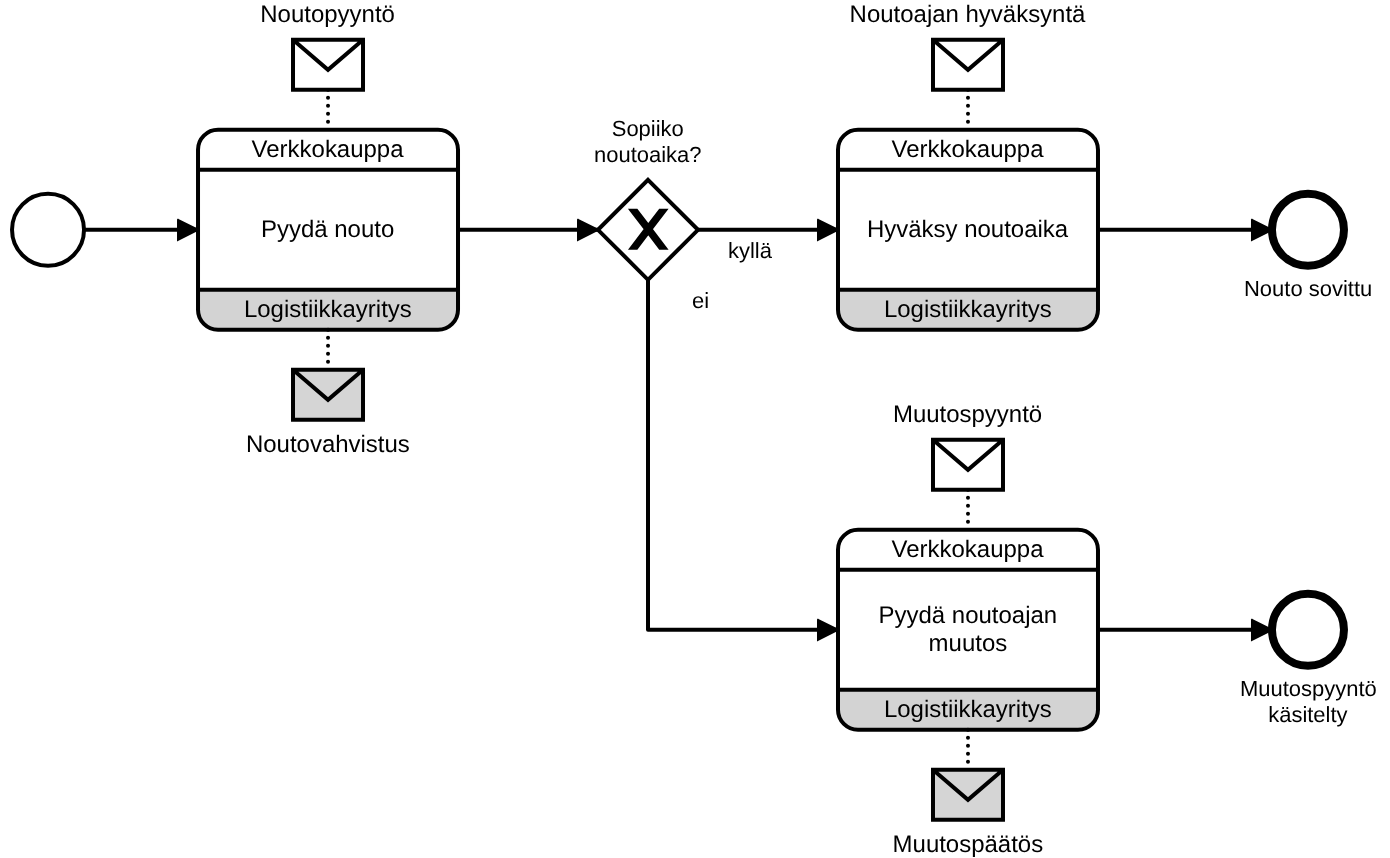
\includegraphics[keepaspectratio]{kuviot/noutokoreografia.png}}

}

\caption{\label{fig-noutokoreografia-teht}Noutopyynnön koreografia}

\end{figure}%

Start Event → koreografiatehtävä \emph{Pyydä nouto} (aloittaja
Verkkokauppa, viesti Noutopyyntö, paluuviesti Noutovahvistus) →
Exclusive Gateway ''Sopiiko noutoaika?''. Haara ''Kyllä'' →
\emph{Hyväksy noutoaika} (Verkkokauppa → Logistiikkayritys, viesti
Noutoajan hyväksyntä) → End Event. Haara ''Ei'' → \emph{Pyydä noutoajan
muutos} (Verkkokauppa → Logistiikkayritys, viesti Muutospyyntö,
paluuviesti Muutospäätös) → End Event.

Tehtävän 43 alkuperäisessä mallissa verkkokauppa ei ilmoita mitään, jos
noutoaika sopii, joten logistiikkayritys ei voi tietää, tuleeko
muutospyyntö vielä. Koreografiassa jokaisen osapuolen on pystyttävä
toimimaan pelkästään saamiensa viestien perusteella. Siksi myös
''Kyllä''-haaraan tarvitaan viesti, jolla verkkokauppa hyväksyy
noutoajan. Portin jälkeisten koreografiatehtävien aloittaja on
verkkokauppa, joka tekee päätöksen ja joka osallistui edelliseen
viestinvaihtoon, joten koreografia noudattaa standardin sääntöjä.

Sisäiset tehtävät, kuten \emph{Tarkista kuljetuskapasiteetti},
\emph{Päätä muutos}, \emph{Päivitä tilaus} ja \emph{Valmistele tilaus
noutoa varten}, eivät näy koreografiassa. Muutoksen hyväksyntä tai
hylkäys näkyy vain muutospäätösviestin sisältönä. Vaihtoehto
hyväksyntäviestille on sopia määräaika, jonka jälkeen noutoaika
katsotaan hyväksytyksi. Silloin osapuolten on kuitenkin luotettava
siihen, että kummankin kello ja tulkinta määräajasta ovat samat.

\end{tcolorbox}

\subsubsection{BPMN-tehtävä 49
(essee)}\label{bpmn-tehtuxe4vuxe4-49-essee}

Kuvan kuva~\ref{fig-koreografia} koreografiassa vain verkkokauppa voi
perua tilauksen. Pohdi, miksi asiakkaan oikeus perua tilaus milloin
tahansa ennen toimitusta olisi koreografiassa ongelmallinen. Millaisilla
säännöillä osapuolet voisivat sopia asiasta niin, että kumpikin tietää
aina, mikä tilanne on?

\begin{tcolorbox}[enhanced jigsaw, arc=.35mm, bottomrule=.15mm, bottomtitle=1mm, breakable, colback=white, colbacktitle=quarto-callout-tip-color!10!white, colframe=quarto-callout-tip-color-frame, coltitle=black, left=2mm, leftrule=.75mm, opacityback=0, opacitybacktitle=0.6, rightrule=.15mm, title=\textcolor{quarto-callout-tip-color}{\faLightbulb}\hspace{0.5em}{Malliratkaisu}, titlerule=0mm, toprule=.15mm, toptitle=1mm]

Jos asiakas saa perua tilauksen milloin tahansa, kaksi osapuolta voi
aloittaa oman viestinvaihtonsa yhtä aikaa: asiakas lähettää peruutuksen
samaan aikaan, kun verkkokauppa lähettää tilauksen matkaan. Kumpikaan ei
tiedä toisen viestistä ennen kuin oma viesti on jo lähetetty, joten
osapuolten käsitys tilauksen tilasta voi erota. Koreografiassa tällaista
kilpatilannetta ei voi esittää yksiselitteisesti. BPMN-standardin mukaan
esimerkiksi tapahtumapohjaisen portin jälkeisillä viestinvaihdoilla on
oltava sama lähettäjä tai sama vastaanottaja, mikä tässä ei täyty.

Mahdollisia sopimuksia:

\begin{itemize}
\tightlist
\item
  \textbf{Määräaika}: peruutus on mahdollinen tietyn ajan tilauksesta,
  minkä jälkeen tilaus käsitellään. Tämä on yksinkertaista, mutta
  edellyttää yhteistä käsitystä ajasta.
\item
  \textbf{Ilmoitus ennen lähetystä}: verkkokauppa ilmoittaa, kun tilaus
  on lähdössä, ja asiakas joko peruu tilauksen tai antaa lähettää sen.
  Päätösvalta on hetkellisesti asiakkaalla, ja koreografia pysyy
  yksiselitteisenä, mutta viestejä tarvitaan enemmän.
\item
  \textbf{Peruutus pyyntönä}: asiakkaan peruutus on pyyntö, johon
  verkkokauppa vastaa joko hyväksymällä sen tai ilmoittamalla, että
  tilaus on jo lähetetty. Viimeinen sana on verkkokaupalla, ja
  myöhästynyt peruutus käsitellään palautuksena.
\end{itemize}

Hyvä vastaus huomaa, että ongelma ei ole mallinnustekninen vaan
liiketoiminnallinen: koreografian laatiminen pakottaa osapuolet sopimaan
asioista, jotka muuten jäisivät epäselviksi.

\end{tcolorbox}

\subsection{Aliprosessit ja toisto}\label{aliprosessit-ja-toisto}

\subsubsection{BPMN-tehtävä 50}\label{bpmn-tehtuxe4vuxe4-50}

Muuttoon kuuluvat seuraavat tehtävät: \emph{Pakkaa laatikot}, \emph{Tee
osoitteenmuutos}, \emph{Kanna tavarat autoon}, \emph{Irtisano
sähkösopimus}, \emph{Aja uuteen osoitteeseen}, \emph{Tee uusi
sähkösopimus}, \emph{Kanna tavarat sisään} ja \emph{Pura laatikot}.
Ryhmittele tehtävät kahteen tai kolmeen aliprosessiin ja mallinna
pääprosessi niin, että aliprosessit on esitetty tiivistettyinä.

\begin{tcolorbox}[enhanced jigsaw, arc=.35mm, bottomrule=.15mm, bottomtitle=1mm, breakable, colback=white, colbacktitle=quarto-callout-tip-color!10!white, colframe=quarto-callout-tip-color-frame, coltitle=black, left=2mm, leftrule=.75mm, opacityback=0, opacitybacktitle=0.6, rightrule=.15mm, title=\textcolor{quarto-callout-tip-color}{\faLightbulb}\hspace{0.5em}{Malliratkaisu}, titlerule=0mm, toprule=.15mm, toptitle=1mm]

Esimerkiksi aliprosessit \emph{Hoida paperityöt} (osoitteenmuutos ja
sähkösopimukset) ja \emph{Siirrä tavarat} (pakkaus, kantaminen, ajo ja
purku). Paperityöt voidaan tehdä rinnakkain tavaroiden siirron kanssa,
joten pääprosessi voi olla muotoa Parallel Gateway → kaksi aliprosessia
→ Parallel Gateway. Tiivistetty aliprosessi merkitään +-merkillä.

\end{tcolorbox}

\subsubsection{BPMN-tehtävä 51}\label{bpmn-tehtuxe4vuxe4-51}

Opettaja arvioi kurssin 25 esseetä. Mallinna tehtävä
Multi-Instance-merkinnällä kahdessa versiossa: (a) opettaja arvioi
esseet yksin, (b) arviointiin osallistuu kolme assistenttia
samanaikaisesti.

\begin{tcolorbox}[enhanced jigsaw, arc=.35mm, bottomrule=.15mm, bottomtitle=1mm, breakable, colback=white, colbacktitle=quarto-callout-tip-color!10!white, colframe=quarto-callout-tip-color-frame, coltitle=black, left=2mm, leftrule=.75mm, opacityback=0, opacitybacktitle=0.6, rightrule=.15mm, title=\textcolor{quarto-callout-tip-color}{\faLightbulb}\hspace{0.5em}{Malliratkaisu}, titlerule=0mm, toprule=.15mm, toptitle=1mm]

\begin{enumerate}
\def\labelenumi{(\alph{enumi})}
\tightlist
\item
  Tehtävä \emph{Arvioi essee}, jossa on Sequential Multi-Instance
  -merkintä (kolme vaakaviivaa). Instanssit suoritetaan yksi kerrallaan.
  (b) Sama tehtävä Parallel Multi-Instance -merkinnällä (kolme
  pystyviivaa). Instanssit suoritetaan rinnakkain. Molemmissa syötteenä
  on esseiden lista, ja prosessi jatkuu vasta, kun kaikki instanssit on
  suoritettu.
\end{enumerate}

\end{tcolorbox}

\subsubsection{BPMN-tehtävä 52
(laajempi)}\label{bpmn-tehtuxe4vuxe4-52-laajempi}

Jaa seuraavat tehtävät aliprosesseiksi. Nimeä aliprosessit loogisella
tavalla ja yhdistä ne toisiinsa järjestysvirroilla. Huomaa, että
tehtävät on esitetty alla aakkosjärjestyksessä, ei välttämättä niiden
suoritusjärjestyksessä.

\begin{itemize}
\tightlist
\item
  Hyvitä maksu
\item
  Kerää ja pakkaa
\item
  Kuittaa maksu
\item
  Käsittele maksun epäonnistuminen
\item
  Käsittele palautus
\item
  Käsittele tilauksen peruutus
\item
  Laske hinta ja verot
\item
  Lähetä lasku
\item
  Lähetä vahvistus asiakkaalle
\item
  Luo lasku
\item
  Luo rahtitarra
\item
  Luo tilausvahvistus
\item
  Luovuta kuljetusyhtiölle
\item
  Päivitä CRM-tilausstatus
\item
  Seuraa lähetystä
\item
  Sovella alennukset
\item
  Sulje tapaus
\item
  Tarkasta petosindikaattorit
\item
  Tarkasta varastotilanne
\item
  Varaa varasto
\item
  Vastaanota tilaus
\item
  Validioi asiakastiedot
\item
  Validioi tilausrivit
\end{itemize}

\begin{tcolorbox}[enhanced jigsaw, arc=.35mm, bottomrule=.15mm, bottomtitle=1mm, breakable, colback=white, colbacktitle=quarto-callout-tip-color!10!white, colframe=quarto-callout-tip-color-frame, coltitle=black, left=2mm, leftrule=.75mm, opacityback=0, opacitybacktitle=0.6, rightrule=.15mm, title=\textcolor{quarto-callout-tip-color}{\faLightbulb}\hspace{0.5em}{Malliratkaisu}, titlerule=0mm, toprule=.15mm, toptitle=1mm]

Yksi mahdollinen jako:

\begin{enumerate}
\def\labelenumi{\arabic{enumi}.}
\tightlist
\item
  \emph{Vastaanota ja tarkasta tilaus}: Vastaanota tilaus, Validioi
  asiakastiedot, Validioi tilausrivit, Tarkasta petosindikaattorit.
\item
  \emph{Hinnoittele tilaus}: Sovella alennukset, Laske hinta ja verot.
\item
  \emph{Varmista saatavuus}: Tarkasta varastotilanne, Varaa varasto.
\item
  \emph{Laskuta ja käsittele maksu}: Luo lasku, Lähetä lasku, Kuittaa
  maksu.
\item
  \emph{Vahvista tilaus}: Luo tilausvahvistus, Lähetä vahvistus
  asiakkaalle, Päivitä CRM-tilausstatus.
\item
  \emph{Toimita tilaus}: Kerää ja pakkaa, Luo rahtitarra, Luovuta
  kuljetusyhtiölle, Seuraa lähetystä.
\item
  \emph{Käsittele poikkeukset}: Käsittele maksun epäonnistuminen,
  Käsittele tilauksen peruutus, Käsittele palautus, Hyvitä maksu.
\end{enumerate}

Pääprosessi: Start Event → 1 → 2 → 3 → 4 → 5 → 6 → \emph{Sulje tapaus} →
End Event. Poikkeukset eivät kuulu normaaliin kulkuun. Ne voidaan
liittää pääprosessiin esimerkiksi Error Boundary Eventillä (maksu
epäonnistui) ja Message Boundary Eventillä tai tapahtuma-aliprosessilla
(peruutus). Palautus käynnistyy yleensä vasta toimituksen jälkeen, joten
se voi olla myös oma erillinen prosessinsa. Muutkin jaot ovat
perusteltavissa, esimerkiksi varaston varaaminen ennen hinnoittelua.

\end{tcolorbox}

\subsubsection{BPMN-tehtävä 53}\label{bpmn-tehtuxe4vuxe4-53}

Mallinna vastaava prosessikulku ilman Loop-tehtävää.

\begin{figure}

\centering{

\pandocbounded{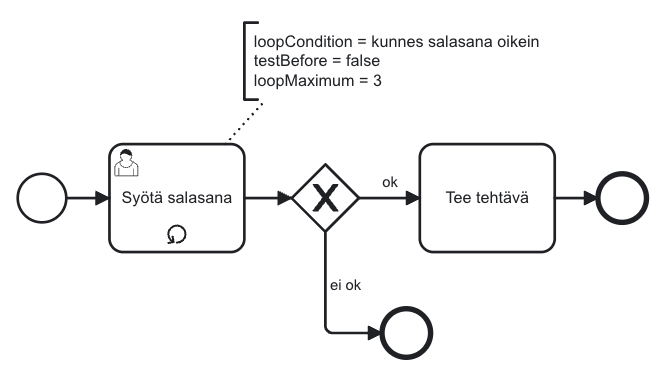
\includegraphics[keepaspectratio]{kuviot/loop.png}}

}

\caption{\label{fig-loop-teht}Ehtoperusteisesti toistettava
Loop-tehtävä}

\end{figure}%

\begin{tcolorbox}[enhanced jigsaw, arc=.35mm, bottomrule=.15mm, bottomtitle=1mm, breakable, colback=white, colbacktitle=quarto-callout-tip-color!10!white, colframe=quarto-callout-tip-color-frame, coltitle=black, left=2mm, leftrule=.75mm, opacityback=0, opacitybacktitle=0.6, rightrule=.15mm, title=\textcolor{quarto-callout-tip-color}{\faLightbulb}\hspace{0.5em}{Malliratkaisu}, titlerule=0mm, toprule=.15mm, toptitle=1mm]

Start Event → Script Task \emph{Nollaa yrityslaskuri} → yhdistävä
Exclusive Gateway → User Task \emph{Syötä salasana} → Script Task
\emph{Kasvata yrityslaskuria} → Exclusive Gateway, josta lähtee kolme
haaraa: \texttt{salasanaOikein} → \emph{Tee tehtävä} → End Event,
\texttt{not\ salasanaOikein\ and\ yritykset\ \textgreater{}=\ 3} → End
Event ''Kirjautuminen epäonnistui'' ja oletusvirta takaisin yhdistävään
porttiin. Koska alkuperäisessä mallissa \texttt{testBefore\ =\ false},
tehtävä suoritetaan vähintään kerran ennen ehdon tarkistamista. Siksi
paluuvirta johdetaan tehtävää edeltävään porttiin, eikä ehtoa tarkisteta
ennen ensimmäistä yritystä.

\end{tcolorbox}

\subsubsection{BPMN-tehtävä 54
(laajempi)}\label{bpmn-tehtuxe4vuxe4-54-laajempi}

Laadi Parallel ja Sequential Multi-instance -tehtäviä käyttävä
prosessimalli, joka pystyy käsittelemään samaan tilaukseen sisältyviä
fyysisiä tuotteita sekä digitaalisten palvelujen käyttöoikeuksia.

\begin{tcolorbox}[enhanced jigsaw, arc=.35mm, bottomrule=.15mm, bottomtitle=1mm, breakable, colback=white, colbacktitle=quarto-callout-tip-color!10!white, colframe=quarto-callout-tip-color-frame, coltitle=black, left=2mm, leftrule=.75mm, opacityback=0, opacitybacktitle=0.6, rightrule=.15mm, title=\textcolor{quarto-callout-tip-color}{\faLightbulb}\hspace{0.5em}{Malliratkaisu}, titlerule=0mm, toprule=.15mm, toptitle=1mm]

Message Start Event ''Tilaus vastaanotettu'' → Parallel Gateway → kaksi
haaraa:

\begin{itemize}
\tightlist
\item
  Fyysiset tuotteet: Sequential Multi-Instance -aliprosessi \emph{Kerää
  tuote} (kolme vaakaviivaa), jonka syötteenä on tilauksen fyysisten
  tuotteiden lista. Keräilijä kerää tuotteet yksi kerrallaan. Sen
  jälkeen \emph{Pakkaa ja lähetä tilaus}.
\item
  Digitaaliset palvelut: Parallel Multi-Instance -tyyppinen Service Task
  \emph{Aktivoi käyttöoikeus} (kolme pystyviivaa), jonka syötteenä on
  käyttöoikeuksien lista. Rajapintakutsut voidaan tehdä samanaikaisesti.
  Sen jälkeen Send Task \emph{Lähetä aktivointitiedot}.
\end{itemize}

Haarat yhdistetään Parallel Gatewaylla → Send Task \emph{Lähetä
tilausvahvistus} → End Event. Jos tilauksessa ei ole lainkaan
jompaakumpaa tuotetyyppiä, Multi-Instance-tehtävä tyhjällä listalla
päättyy heti. Vaihtoehtoisesti haarat voi jakaa Inclusive Gatewaylla
tuotetyyppien mukaan.

\end{tcolorbox}

\subsubsection{BPMN-tehtävä 55}\label{bpmn-tehtuxe4vuxe4-55}

Mallinna työpisteen siivous Ad-hoc-aliprosessina. Aliprosessiin kuuluvat
tehtävät \emph{Tyhjennä roskakori}, \emph{Pyyhi pöytä}, \emph{Järjestä
paperit}, \emph{Imuroi lattia} ja \emph{Kastele kasvit}. Tehtävät voi
tehdä missä järjestyksessä tahansa, eikä kaikkia tarvitse tehdä joka
kerta. Mitä etuja ja haittoja Ad-hoc-aliprosessilla on verrattuna
siihen, että tehtävät mallinnettaisiin kiinteään järjestykseen? Missä
tilanteissa Ad-hoc-rakenne voisi soveltua tekoälyagentin ohjaamaan
prosessiin?

\begin{tcolorbox}[enhanced jigsaw, arc=.35mm, bottomrule=.15mm, bottomtitle=1mm, breakable, colback=white, colbacktitle=quarto-callout-tip-color!10!white, colframe=quarto-callout-tip-color-frame, coltitle=black, left=2mm, leftrule=.75mm, opacityback=0, opacitybacktitle=0.6, rightrule=.15mm, title=\textcolor{quarto-callout-tip-color}{\faLightbulb}\hspace{0.5em}{Malliratkaisu}, titlerule=0mm, toprule=.15mm, toptitle=1mm]

Ad-hoc-aliprosessi \emph{Siivoa työpiste} merkitään
\textasciitilde-merkillä, ja sen sisällä on viisi tehtävää ilman
järjestysvirtoja. Aliprosessi päättyy, kun siivoaja toteaa siivouksen
valmiiksi (päättymisehto).

Edut: malli on pieni ja vastaa todellisuutta, jossa järjestys ja tarve
vaihtelevat. Tekijä voi käyttää harkintaa. Haitat: malli ei takaa, että
tietyt tehtävät tehdään. Järjestystä tai riippuvuuksia ei voi esittää.
Suorituksen seuranta ja mittaaminen vaikeutuvat, ja kaikki
prosessimoottorit eivät tue ad-hoc-aliprosesseja.

Tekoälyagentti: ad-hoc-aliprosessin tehtävät voivat toimia agentin
käytettävissä olevina työkaluina. Agentti päättää tilanteen perusteella,
mitä tehtäviä se kutsuu ja missä järjestyksessä. Ympäröivä prosessi
pitää huolen siitä, mitä tapahtuu ennen agenttia ja sen jälkeen. Rakenne
sopii esimerkiksi asiakaspalvelupyyntöjen käsittelyyn, jossa tarvittavat
tiedonhaut ja toimenpiteet vaihtelevat tapauksittain.

\end{tcolorbox}

\subsection{Kokoavia tehtäviä}\label{kokoavia-tehtuxe4viuxe4}

\subsubsection{BPMN-tehtävä 56}\label{bpmn-tehtuxe4vuxe4-56}

Kirjaston asiakas tilaa kaukolainan. Kirjasto lähettää pyynnön toiselle
kirjastolle ja odottaa kirjaa enintään 14 päivää. Jos kirja saapuu,
asiakkaalle ilmoitetaan noudettavasta kirjasta. Jos kirjaa ei kuulu,
asiakkaalle ilmoitetaan, ettei kirjaa saatu. Mallinna kirjaston prosessi
ja lainaavan kirjaston osuus suljettuna altaana.

\begin{tcolorbox}[enhanced jigsaw, arc=.35mm, bottomrule=.15mm, bottomtitle=1mm, breakable, colback=white, colbacktitle=quarto-callout-tip-color!10!white, colframe=quarto-callout-tip-color-frame, coltitle=black, left=2mm, leftrule=.75mm, opacityback=0, opacitybacktitle=0.6, rightrule=.15mm, title=\textcolor{quarto-callout-tip-color}{\faLightbulb}\hspace{0.5em}{Malliratkaisu}, titlerule=0mm, toprule=.15mm, toptitle=1mm]

Kirjaston allas: Message Start Event ''Kaukolainapyyntö saapunut'' →
Send Task \emph{Lähetä pyyntö lainaavalle kirjastolle} → Event-Based
Gateway, jota seuraa Message Intermediate Catch Event ''Kirja saapunut''
→ \emph{Ilmoita asiakkaalle noudettavasta kirjasta} sekä Timer
Intermediate Catch Event \texttt{P14D} → \emph{Ilmoita asiakkaalle,
ettei kirjaa saatu}. Lainaava kirjasto on suljettu allas, johon ja josta
kulkevat viestivirrat.

\end{tcolorbox}

\subsubsection{BPMN-tehtävä 57}\label{bpmn-tehtuxe4vuxe4-57}

Verkkopalveluun kirjaudutaan kaksivaiheisesti. Käyttäjä syöttää
salasanan, ja jos se on oikein, hänen puhelimeensa lähetetään
vahvistuskoodi. Jos käyttäjä syöttää koodin viiden minuutin kuluessa,
kirjautuminen onnistuu. Muuten kirjautuminen keskeytetään. Väärästä
salasanasta käyttäjälle näytetään virheilmoitus. Mallinna prosessi.

\begin{tcolorbox}[enhanced jigsaw, arc=.35mm, bottomrule=.15mm, bottomtitle=1mm, breakable, colback=white, colbacktitle=quarto-callout-tip-color!10!white, colframe=quarto-callout-tip-color-frame, coltitle=black, left=2mm, leftrule=.75mm, opacityback=0, opacitybacktitle=0.6, rightrule=.15mm, title=\textcolor{quarto-callout-tip-color}{\faLightbulb}\hspace{0.5em}{Malliratkaisu}, titlerule=0mm, toprule=.15mm, toptitle=1mm]

Start Event → User Task \emph{Syötä salasana} → Exclusive Gateway
''Salasana oikein?''. Haara ''Ei'' → \emph{Näytä virheilmoitus} → End
Event. Haara ''Kyllä'' → Send Task \emph{Lähetä vahvistuskoodi} →
Event-Based Gateway, jota seuraa Message Intermediate Catch Event
''Koodi syötetty'' → \emph{Kirjaa käyttäjä sisään} → End Event sekä
Timer Intermediate Catch Event \texttt{PT5M} → \emph{Keskeytä
kirjautuminen} → End Event. Vaihtoehtoisesti koodin syöttäminen voi olla
User Task, johon liitetään keskeyttävä Timer Boundary Event.

\end{tcolorbox}

\bookmarksetup{startatroot}

\chapter{Työvälineitä}\label{tyuxf6vuxe4lineituxe4}

Seuraavassa esitellään lyhyesti työvälineet, joita kirjan esimerkeissä
on käytetty. Voit hyödyntää niitä myös harjoitustehtäviä tehdessäsi.
Kaikki esitellyt välineet ovat maksuttomia tai niistä on saatavilla myös
maksuton versio. Välineet kehittyvät jatkuvasti, joten käyttöliittymät
ja ominaisuudet saattavat poiketa jonkin verran kirjan kuvista.

\section{Camunda}\label{camunda}

\emph{Camunda} on BPMN-, DMN- ja työnkulkualusta, jolla prosessimalleja
voi paitsi laatia prosessiamalleja, ne voidaan myös suorittaa.

\subsection{Camunda Modeler}\label{camunda-modeler}

\emph{Camunda Modeler}in avulla voidaan luoda BPMN- ja DMN-malleja sekä
määritellä yksityiskohtaisesti tehtävien ominaisuuksia (esim.
FEEL-lausekkeet, Service Task -määrittelyt, ajastimet). Mallit
tallentuvat .bpmn-tiedostoina (BPMN XML), jotka voidaan avata myös
muissa BPMN-välineissä. Camunda Modeler on maksuton avoimen lähdekoodin
työpöytäsovellus, joka on saatavilla Windows-, macOS- ja
Linux-ympäristöihin.

\subsection{Camundan verkkoversio}\label{camundan-verkkoversio}

Camundasta on myös verkkoselaimessa toimiva Web Modeler. Web Modelerilla
tehdyt mallit tallentuvat pilveen ja ne voidaan jakaa muille valituille
käyttäjille.

\section{Token Simulation}\label{token-simulation}

Prosessimallin toimintaa voi olla vaikea hahmottaa pelkästään kuvaa
katsomalla, varsinkin jos mallissa on rinnakkaisia polkuja, tapahtumia
tai monimutkaisia portteja. \emph{Token Simulation} on bpmn.io-projektin
kehittämä apuväline, jolla prosessin kulkua voi seurata animaationa:
prosessin käynnistävästä tapahtumasta lähtee liikkeelle merkki
(\emph{token}), joka kulkee prosessin läpi järjestysvirtoja pitkin.
Porteissa voit itse valita, mihin suuntaan merkki jatkaa, ja
rinnakkaisissa haaroissa näet, miten merkki jakautuu ja yhdistyy
uudelleen. Sen avulla voit testata, toimiiko mallisi kuten olit
ajatellut -- päättyykö se oikein kaikissa vaihtoehtoisissa kuluissa vai
jääkö prosessi esimerkiksi jumiin jonkin portin kohdalle.

Token Simulationia voi käyttää kolmella tavalla:

\begin{enumerate}
\def\labelenumi{\arabic{enumi}.}
\tightlist
\item
  Selaimessa ilman asennusta osoitteessa
  \url{https://bpmn-io.github.io/bpmn-js-token-simulation/}. Voit avata
  sivulla oman .bpmn-tiedostosi raahaamalla sen selainikkunaan.
\item
  Camundan verkkoversiossa, jossa simulaatio on valmiiksi mukana.
\item
  Camunda Modelerin lisäosana, joka asennetaan plugin-lisäosana.
\end{enumerate}

\section{Draw.io}\label{draw.io}

\emph{Draw.io} on maksuton yleiskäyttöinen kaaviotyökalu. Se on
käytettävissä selaimella sekä työpöytäsovelluksena. Draw.io sisältää
BPMN- ja ArchiMate-symbolikirjastot (More Shapes -\textgreater{} BPMN /
ArchiMate 3). Väline sopii nopeisiin luonnoksiin, prosessikarttoihin,
vuokaavioihin ja muihin kuin BPMN-kuvauksiin.

Huomaa, että Draw.io piirtää ainoastaan kuvia. Sen avulla ei voi tehdä
suoritettavia malleja. BPMN-sääntöjä ei tarkisteta eikä mallia voi
simuloida tai suorittaa, toisin kuin esimerkiksi Camunda Modelerissa.

\section{Archi}\label{archi}

\emph{Archi} on maksuton, avoimen lähdekoodin ArchiMate-mallinnusväline
kokokonaisarkkitehtuurin mallintamiseen. Se on saatavilla Windows-,
macOS- ja Linux-ympäristöihin.

\bookmarksetup{startatroot}

\chapter*{Lähteet}\label{luxe4hteet}
\addcontentsline{toc}{chapter}{Lähteet}

\markboth{Lähteet}{Lähteet}

\protect\phantomsection\label{refs}
\begin{CSLReferences}{1}{1}
\bibitem[\citeproctext]{ref-adeoye2021research}
Adeoye-Olatunde, Omolola A, ja Nicole L Olenik. 2021. {''Research and
scholarly methods: Semi-structured interviews''}. \emph{Journal of the
american college of clinical pharmacy} 4 (10): 1358--67.

\bibitem[\citeproctext]{ref-best2006walter}
Best, Mark, ja Duncan Neuhauser. 2006. {''Walter A Shewhart, 1924, and
the Hawthorne factory''}. \emph{Quality and Safety in Health Care} 15
(2): 142--43.

\bibitem[\citeproctext]{ref-bourne2002success}
Bourne, Mike, Andy Neely, Ken Platts, ja John Mills. 2002. {''The
success and failure of performance measurement initiatives: Perceptions
of participating managers''}. \emph{International journal of operations
\& production management} 22 (11): 1288--310.

\bibitem[\citeproctext]{ref-brynjolfsson1993productivity}
Brynjolfsson, Erik. 1993. {''The productivity paradox of information
technology''}. \emph{Communications of the ACM} 36 (12): 66--77.

\bibitem[\citeproctext]{ref-cardoso2009requirements}
Cardoso, Evellin Cristine Souza, João Paulo A Almeida, ja Giancarlo
Guizzardi. 2009. {''Requirements engineering based on business process
models: A case study''}. \emph{2009 13th Enterprise Distributed Object
Computing Conference Workshops}, 320--27.

\bibitem[\citeproctext]{ref-cocskun2022erp}
Coşkun, Evren, Bahar Gezici, Murat Aydos, Ayça Kolukısa Tarhan, ja Vahid
Garousi. 2022. {''ERP failure: A systematic mapping of the
literature''}. \emph{Data \& Knowledge Engineering} 142: 102090.

\bibitem[\citeproctext]{ref-davenport1990new}
Davenport, Thomas H, ja James E Short. 1990. \emph{The new industrial
engineering: information technology and business process redesign}.

\bibitem[\citeproctext]{ref-deming1982quality}
Deming, W. Edwards. 1982. \emph{Quality, Productivity, and Competitive
Position}. Massachusetts Institute of Technology, Center for Advanced
Engineering Study.

\bibitem[\citeproctext]{ref-dijkman2011road}
Dijkman, RM, ITP Vanderfeesten, ja Hajo A Reijers. 2011. \emph{The road
to a business process architecture: an overview of approaches and their
use}.

\bibitem[\citeproctext]{ref-eid2012business}
Eid-Sabbagh, Rami-Habib, Remco Dijkman, ja Mathias Weske. 2012.
{''Business process architecture: use and correctness''}.
\emph{International Conference on Business Process Management}, 65--81.

\bibitem[\citeproctext]{ref-finney2007erp}
Finney, Sherry, ja Martin Corbett. 2007. {''ERP implementation: a
compilation and analysis of critical success factors''}. \emph{Business
process management journal} 13 (3): 329--47.

\bibitem[\citeproctext]{ref-ford2021my}
Ford, Henry. 2021. \emph{My life and work}. Phoemixx Classics Ebooks.

\bibitem[\citeproctext]{ref-fulkerson1962expected}
Fulkerson, D Ray. 1962. {''Expected critical path lengths in PERT
networks''}. \emph{Operations Research} 10 (6): 808--17.

\bibitem[\citeproctext]{ref-georgakopoulos1995overview}
Georgakopoulos, Diimitrios, Mark Hornick, ja Amit Sheth. 1995. {''An
overview of workflow management: From process modeling to workflow
automation infrastructure''}. \emph{Distributed and parallel Databases}
3 (2): 119--53.

\bibitem[\citeproctext]{ref-gonzalez2019business}
Gonzalez-Lopez, Fernanda, ja Guillermo Bustos. 2019. {''Business process
architecture design methodologies--a literature review''}.
\emph{Business Process Management Journal} 25 (6): 1317--34.

\bibitem[\citeproctext]{ref-gronroos1982applied}
Grönroos, Christian. 1982. {''An applied service marketing theory''}.
\emph{European journal of marketing} 16 (7): 30--41.

\bibitem[\citeproctext]{ref-hamel1990core}
Hamel, G., ja C. K. Prahalad. 1990. {''The core competence of the
corporation''}. \emph{Harvard Business Review} 68 (3): 79--91.

\bibitem[\citeproctext]{ref-hammer2007}
Hammer, Michael. 2007. {''The Process Audit''}. \emph{Harvard Business
Review} 85 (4): 111--23.

\bibitem[\citeproctext]{ref-hammer2009reengineering}
Hammer, Michael, ja James Champy. 2009. \emph{Reengineering the
corporation: Manifesto for business revolution, a}. Zondervan.

\bibitem[\citeproctext]{ref-harmon2019business}
Harmon, Paul. 2019. \emph{Business process change: a business process
management guide for managers and process professionals}. Morgan
Kaufmann.

\bibitem[\citeproctext]{ref-herbane2004business}
Herbane, Brahim, Dominic Elliott, ja Ethné M Swartz. 2004. {''Business
continuity management: time for a strategic role?''} \emph{Long range
planning} 37 (5): 435--57.

\bibitem[\citeproctext]{ref-hiatt2006adkar}
Hiatt, Jeff. 2006. \emph{ADKAR: A model for change in business,
government, and our community}. Prosci.

\bibitem[\citeproctext]{ref-idogawa2023critical}
Idogawa, Juliano, Flávio Santino Bizarrias, ja Ricardo Câmara. 2023.
{''Critical success factors for change management in business process
management''}. \emph{Business Process Management Journal} 29 (7):
2009--33.

\bibitem[\citeproctext]{ref-juran1951quality}
Juran, Joseph M. 1951. \emph{Quality-Control Handbook}. McGraw-Hill.

\bibitem[\citeproctext]{ref-keen1981information}
Keen, Peter GW. 1981. {''Information systems and organizational
change''}. \emph{Communications of the ACM} 24 (1): 24--33.

\bibitem[\citeproctext]{ref-kemppainen2018}
Kemppainen, R. 2018. {''Hyvä ja laadukas työohje''}. Insinöörityö,
Automaatiotekniikka, Metropolia Ammattikorkeakoulu.

\bibitem[\citeproctext]{ref-kemppainen2024prosessien}
Kemppainen, Ville. 2024. {''Prosessien automatisointi
ohjelmistorobotiikalla pk-yrityksess{ä}''}. University of Jyv{ä}skyl{ä}.

\bibitem[\citeproctext]{ref-klerkx2013interaction}
Klerkx, Laurens, ja Noelle Aarts. 2013. {''The interaction of multiple
champions in orchestrating innovation networks: Conflicts and
complementarities''}. \emph{Technovation} 33 (6-7): 193--210.

\bibitem[\citeproctext]{ref-kotter2007leading}
{Kotter, John P ym.} 2007. \emph{Leading change: Why transformation
efforts fail}.

\bibitem[\citeproctext]{ref-langley2007process}
Langley, Ann. 2007. {''Process thinking in strategic organization''}.
\emph{Strategic organization} 5 (3): 271--82.

\bibitem[\citeproctext]{ref-leshob2018towards}
Leshob, Abderrahmane, Audrey Bourgouin, ja Laurent Renard. 2018.
{''Towards a process analysis approach to adopt robotic process
automation''}. \emph{2018 IEEE 15th international conference on
e-business engineering (ICEBE)}, 46--53.

\bibitem[\citeproctext]{ref-mcivor2000practical}
McIvor, Ronan. 2000. {''A practical framework for understanding the
outsourcing process''}. \emph{Supply Chain Management: an international
journal} 5 (1): 22--36.

\bibitem[\citeproctext]{ref-medina1992action}
Medina-Mora, Raul, Terry Winograd, Rodrigo Flores, ja Fernando Flores.
1992. {''The action workflow approach to workflow management
technology''}. \emph{Proceedings of the 1992 ACM conference on
Computer-supported cooperative work}, 281--88.

\bibitem[\citeproctext]{ref-mendling2007understanding}
Mendling, Jan, Gustaf Neumann, ja Wil Van Der Aalst. 2007.
{''Understanding the occurrence of errors in process models based on
metrics''}. \emph{OTM Confederated International Conferences" On the
Move to Meaningful Internet Systems"}, 113--30.

\bibitem[\citeproctext]{ref-mendling2010seven}
Mendling, Jan, Hajo A Reijers, ja Wil MP van der Aalst. 2010. {''Seven
process modeling guidelines (7PMG)''}. \emph{Information and software
technology} 52 (2): 127--36.

\bibitem[\citeproctext]{ref-niemi2024kokonaisarkkitehtuuri}
Niemi, E. 2024. {''Kokonaisarkkitehtuuri: Oppaasi organisaation
muutosmatkalla''}. \emph{Alma Insights}.

\bibitem[\citeproctext]{ref-nonaka1996theory}
Nonaka, Lkujiro, Hirotaka Takeuchi, ja Katsuhiro Umemoto. 1996. {''A
theory of organizational knowledge creation''}. \emph{International
journal of technology Management} 11 (7-8): 833--45.

\bibitem[\citeproctext]{ref-ogden1923meaning}
Ogden, Charles Kay, ja Ivor Armstrong Richards. 1923. \emph{The Meaning
of Meaning: A Study of the Influence of Language Upon Thought and of the
Science of Symbolism}. Harcourt, Brace \& Co.

\bibitem[\citeproctext]{ref-osterwalder2004}
Osterwalder, Alexander. 2004. {''The Business Model Ontology: A
Proposition in a Design Science Approach''}. Tohtorinväitöskirja,
Université de Lausanne.

\bibitem[\citeproctext]{ref-panayiotou2015business}
Panayiotou, Nikolaos A, Sotiris P Gayialis, Nikolaos P Evangelopoulos,
ja Petros K Katimertzoglou. 2015. {''A business process modeling-enabled
requirements engineering framework for ERP implementation''}.
\emph{Business Process Management Journal} 21 (3): 628--64.

\bibitem[\citeproctext]{ref-parmenter2010key}
Parmenter, David. 2010. \emph{Key performance indicators (KPI):
developing, implementing, and using winning KPIs}. John Wiley \& Sons.

\bibitem[\citeproctext]{ref-paulk1993}
Paulk, Mark C., Bill Curtis, Mary Beth Chrissis, ja Charles V. Weber.
1993. {''Capability Maturity Model, Version 1.1''}. \emph{IEEE Software}
10 (4): 18--27.

\bibitem[\citeproctext]{ref-Proctor2018WhyDoBPR}
Proctor, James. 2018. {''Why Do Business Process Reengineering
Initiatives Fail to Deliver Transformative Results?''} Inteq Group,
lokakuuta 22.
\url{https://www.inteqgroup.com/blog/why-do-business-process-reengineering-initiatives-fail}.

\bibitem[\citeproctext]{ref-prucha2025llm}
Průcha, Petr, Michaela Matoušková, ja Jan Strnad. 2025. \emph{Are LLM
Agents the New RPA? A Comparative Study with RPA Across Enterprise
Workflows}. \url{https://arxiv.org/abs/2509.04198}.

\bibitem[\citeproctext]{ref-rassfeld2013integrated}
Raßfeld, Colin, Dominik Rößle, ja Roland Jochem. 2013. {''Integrated and
modular design of an optimized process architecture''}.
\emph{International Journal of Production Management and Engineering} 1
(1): 63--75.

\bibitem[\citeproctext]{ref-ridgway1956dysfunctional}
Ridgway, Valentine F. 1956. {''Dysfunctional consequences of performance
measurements''}. \emph{Administrative science quarterly} 1 (2): 240--47.

\bibitem[\citeproctext]{ref-rosemann2006process}
Rosemann, Michael. 2006. {''Process portfolio management''}.
\emph{BPTrends. April}.

\bibitem[\citeproctext]{ref-rosemann2005}
Rosemann, Michael, ja Tonia de Bruin. 2005. {''Towards a Business
Process Management Maturity Model''}. \emph{Proceedings of the 13th
European Conference on Information Systems (ECIS 2005)} (Regensburg).

\bibitem[\citeproctext]{ref-roglinger2012}
Röglinger, Maximilian, Jens Pöppelbuß, ja Jörg Becker. 2012. {''Maturity
Models in Business Process Management''}. \emph{Business Process
Management Journal} 18 (2): 328--46.

\bibitem[\citeproctext]{ref-schonreiter2018methodologies}
Schönreiter, Irene Maria. 2018. {''Methodologies for process
harmonization in the post-merger integration phase: A literature
review''}. \emph{Business Process Management Journal} 24 (2): 330--56.

\bibitem[\citeproctext]{ref-shamsuzzoha2025robotic}
Shamsuzzoha, Ahm, ja Sini Pelkonen. 2025. {''A robotic process
automation model for order-handling optimization in supply chain
management''}. \emph{Supply Chain Analytics} 9: 100102.

\bibitem[\citeproctext]{ref-syed2020robotic}
Syed, Rehan, Suriadi Suriadi, Michael Adams, ym. 2020. {''Robotic
process automation: contemporary themes and challenges''}.
\emph{Computers in industry} 115: 103162.

\bibitem[\citeproctext]{ref-taylor1911principles}
Taylor, Frederick Winslow. 1911. \emph{The principles of scientific
management}. NuVision Publications, LLC.

\bibitem[\citeproctext]{ref-togaf-kyvykkyydet}
The Open Group. 2022. \emph{TOGAF Series Guide: Business Capabilities}.
The Open Group.

\bibitem[\citeproctext]{ref-tiirikainen2008johtaja}
Tiirikainen, Vesa. 2008. {''Johtaja: ole IT-strategi''}. \emph{Helsinki:
Talentum}.

\bibitem[\citeproctext]{ref-van2016data}
Van Der Aalst, Wil. 2016. {''Data science in action''}. Teoksessa
\emph{Process mining: Data science in action}. Springer.

\bibitem[\citeproctext]{ref-williamson1975markets}
Williamson, Oliver E. 1975. {''Markets and hierarchies: analysis and
antitrust implications: a study in the economics of internal
organization''}. \emph{University of Illinois at Urbana-Champaign's
Academy for Entrepreneurial Leadership Historical Research Reference in
Entrepreneurship}.

\bibitem[\citeproctext]{ref-von1968general}
{Von Bertalanffy, Ludwig ym.} 1968. {''General system theory''}.
\emph{New York} 41973 (1968): 40.

\bibitem[\citeproctext]{ref-ye2023proagent}
Ye, Yining, Xin Cong, Shizuo Tian, ym. 2023. \emph{ProAgent: From
Robotic Process Automation to Agentic Process Automation}.
\url{https://arxiv.org/abs/2311.10751}.

\end{CSLReferences}




\end{document}
